%%%%%%%%%%%%%%%%%%%%%%%%
%% Sample use of the infthesis class to prepare a thesis. This can be used as 
%% a template to produce your own thesis.
%%
%% The title, abstract and so on are taken from Martin Reddy's csthesis class
%% documentation.
%%
%% MEF, October 2002
%%%%%%%%%%%%%%%%%%%%%%%%

%%%%
%% Load the class. Put any options that you want here (see the documentation
%% for the list of options). The following are samples for each type of
%% thesis:
%%
%% Note: you can also specify any of the following options:
%%  logo: put a University of Edinburgh logo onto the title page
%%  frontabs: put the abstract onto the title page
%%  deptreport: produce a title page that fits into a Computer Science
%%      departmental cover [not sure if this actually works]
%%  singlespacing, fullspacing, doublespacing: choose line spacing
%%  oneside, twoside: specify a one-sided or two-sided thesis
%%  10pt, 11pt, 12pt: choose a font size
%%  centrechapter, leftchapter, rightchapter: alignment of chapter headings
%%  sansheadings, normalheadings: headings and captions in sans-serif
%%      (default) or in the same font as the rest of the thesis
%%  [no]listsintoc: put list of figures/tables in table of contents (default:
%%      not)
%%  romanprepages, plainprepages: number the preliminary pages with Roman
%%      numerals (default) or consecutively with the rest of the thesis
%%  parskip: don't indent paragraphs, put a blank line between instead
%%  abbrevs: define a list of useful abbreviations (see documentation)
%%  draft: produce a single-spaced, double-sided thesis with narrow margins
%%
%% For a PhD thesis -- you must also specify a research institute:
\documentclass[phd,icsa,twoside]{infthesis}

%% For an MPhil thesis -- also needs an institute
% \documentclass[mphil,ianc]{infthesis}

%% MSc by Research, which also needs an institute
% \documentclass[mscres,irr]{infthesis}

%% Taught MSc -- specify a particular degree instead. If none is specified,
%% "MSc in Informatics" is used.
% \documentclass[msc,cogsci]{infthesis}
% \documentclass[msc]{infthesis}  % for the MSc in Informatics

%% Master of Informatics (5 year degree)
% \documentclass[minf]{infthesis}

%% Undergraduate project -- specify the degree course and project type
%% separately
% \documentclass[bsc]{infthesis}
% \course{Artificial Intelligence and Psychology}
% \project{Fourth Year Project Report}

%% Put any \usepackage commands you want to use right here; the following is 
%% an example:
\usepackage[section]{placeins}
\usepackage{pdflscape}
\usepackage{url}
\usepackage{amsmath}
\usepackage{graphicx}
\usepackage{subfig}
\usepackage{multicol}
\usepackage{lipsum}
\usepackage{siunitx}
\usepackage{booktabs}
\usepackage[table]{xcolor}
\usepackage{booktabs}
\usepackage{xspace}
\usepackage{balance}
\usepackage{listings}
\usepackage{lstlinebgrd}
\usepackage[]{algorithm2e} 
\usepackage{algpseudocode}

\newlength\llength
\usepackage{stackengine}
\usepackage{rotating}
\usepackage{booktabs} % For formal tables
\usepackage{textcomp}
\definecolor{listinggray}{gray}{0.9}
\definecolor{lbcolor}{rgb}{0.9,0.9,0.9}
\usepackage{subfig}
\usepackage{verbatim}
\usepackage[titletoc]{appendix}
\usepackage[normalem]{ulem}
\usepackage{amsmath}
\usepackage{mathtools}
\usepackage{xspace} 
\usepackage{float}
\DeclarePairedDelimiter\ceil{\lceil}{\rceil}
\DeclarePairedDelimiter\floor{\lfloor}{\rfloor}
\usepackage{todonotes}
\SetKwComment{Comment}{$\triangleright$\ }{}
\renewcommand{\theparagraph}{\arabic{paragraph}}
\newcommand{\ie}{i.\,e.\xspace}
\newcommand{\eg}{e.\,g.\xspace}
\newcommand{\bench}[1]{\textit{#1}\xspace}
\usepackage[labelfont=bf]{caption}
%% Information about the title, etc.
\title{From Software to Hardware: Making Dynamic Multicore Processors Practical}
\author{Paul-Jules Micolet}

%% If the year of submission is not the current year, uncomment this line and 
%% specify it here:
% \submityear{1785}

%% Optionally, specify the graduation month and year:
% \graduationdate{February 1786}

%% Specify the abstract here.
\abstract{%
Heterogeneous processors such as ARM's big.LITTLE have become popular as they offer a choice between performance and energy efficiency.
However, the core configurations are fixed at design time which offers a limited amount of adaptation. 
Dynamic Multicore Processors (DMPs) bridge the gap between homogeneous and fully reconfigurable systems.
They present a new way of improving single-threaded performance by running a thread on groups of cores (compositions) and with the ability of changing the processor topology on the fly, they can better adapt themselves to any task at hand.
However, these potential performance improvements are made difficult due to two main challenges: the difficulty of determining a processor configuration that leads to the optimal performance and knowing how to tackle hardware bottlenecks that may impede the performance of composition.

This thesis first demonstrates that ahead-of-time thread and core partitioning used to improve the performance of multithreaded programs can be automated. 
This is done by analysing static code features to generate a machine-learning model that determines a processor configuration that leads to good performance for an application. 
The machine learning model is able to predict a configuration that is within 16\% of the performance of the best configuration from the search space.

This is followed by studying how dynamically adapting the size of a composition at runtime can be used to reduce energy consumption whilst maintaining the same speedup as the fastest static core composition.
An analysis of how much energy can be saved by adapting the size of the composition at runtime is conducted, showing that dynamic reconfiguration can reduce energy consumption by 42\% on average.
A model is then built using linear regression which analyses the features of basic blocks being executed to determine if the current composition should be reconfigured; on average it reduces energy consumption by 37\%.

Finally the hardware mechanisms that drive core composition are explored.
A new fetching mechanism for core composition is proposed, where cores fetch code in a round-robin fashion.
The use of value prediction is also motivated, as large core compositions are more susceptible to data-dependencies.
This new hardware setup shows massive potential.
By exploring a perfect value predictor with perfect branch prediction and the new fetching scheme, the performance of a large core composition can be improved by a factor of up to 3x, and 1.88x on average.
Furthermore, this thesis shows that state-of-the-art value prediction with a normal branch predictor still leads to good performance improvements, with an average of 1.33x to up to 2.7x speedup.
}

\layman{
As computers become more and more powerful, the main component that drives this performance --- the central processing unit --- is becoming harder to improve on due to a multitude of reasons.
In order to compensate for the fact processor designers cannot increase the performance of a single processor core; the common philosophy has been to pack multiple copies of smaller cores into a single package.
Whilst this approach has been successful to a certain degree, some applications cannot benefit from spreading their computation on multiple processor cores but instead perform best on larger cores.
To compensate for this, hardware designers propose heterogeneous processors where different types of cores are on the same package.
However, this still requires that the design of the processor be determined before it is built.
This reduces the flexibility of the system and thus may potentially limit performance on some applications.
Therefore, a new processor model was created, one where the cores can be grouped together at any time in order to form larger cores: these processors are called Dynamic Multicore Processors (DMPs).
DMPs can adapt themselves to the needs of the program at hand which helps improve the performance of the program.

This thesis explores how to determine ways in which the DMP can automatically reconfigure itself to adapt to the needs of the program at hand.
Whilst previous research has looked into ways of reconfiguring the processor using hand-crafted algorithms, this is not an efficient solution as it requires intimate knowledge of the processor and is time consuming.
Automating this process makes these types of processors more accessible, as programmers will not have to think about the underlying hardware when they write their programs.
The reconfiguration can be used to either make the programs execute faster, or consume less energy.
This thesis shows that reconfiguring the processor can be fully automated through the use of machine learning, thus removing the need of hand-crafting an algorithm.
Finally, the mechanisms that determine how the processor functions once reconfigured are analysed to see if any improvements can be made.
By modifying the way the processor behaves, the performance of programs can be improved even more.
This motivates further research in these types of processors.


}
	%% Now we start with the actual document.
\begin{document}

%% First, the preliminary pages
\begin{preliminary}

%% This creates the title page
\maketitle

%% Acknowledgements
%\begin{acknowledgements}

%Many thanks to my mummy for the numerous packed lunches; and of course to
%Igor, my faithful lab assistant.
%\end{acknowledgements}

%% Next we need to have the declaration.
\standarddeclaration

%% Finally, a dedication (this is optional -- uncomment the following line if
%% you want one).
% \dedication{To my mummy.}

%% Create the table of contents
\tableofcontents

%% If you want a list of figures or tables, uncomment the appropriate line(s)
% \listoffigures
% \listoftables

\end{preliminary}

%%%%%%%%
%% Include your chapter files here. See the sample chapter file for the basic
%% format.
\chapter{Introduction}
%From StreamIt paper
Multicore processors are now common in all computing systems ranging from mobile devices to data centers.
As advances in single threaded performance have slowed, multicore processors have offered a way to use the increasing numbers of transistors available.
However, designing processors that scale to a large number of cores is difficult and a shift towards tiled architecture seems inevitable.
A tiled architecture such as Tilera~\cite{bell2008tile} or Raw~\cite{waingold1997raw} is composed of smaller simpler cores that are placed on a regular grid.
This improves hardware scalability and enables multi-threaded applications to exploit the large core count.

% Tiled architecture problem: cores too weak => need reconfiguration
However, workloads that require high single threaded performance are penalized by the simple nature of each core~\cite{eyerman2010amdahl}.
One solution to this problem is heterogeneous multicores which utilize cores with different levels of power and performance.
Although heterogeneous multicores are common place in mobile devices, they have little reconfiguration or adaptive capabilities (\eg only two type of cores available for ARM big.LITTLE).
Dynamic multicore processors offer a solution to this problem by allowing cores to compose (or fuse) together~\cite{ipek2007CoreFusion} into larger logical cores to accelerate single threads.
This produces ``on-demand'' heterogeneity where cores are grouped to adapt to the workload's demand.

\section{The Problem}

\paragraph*{Dynamic multicore processor reconfiguration}
Whilst there exists a multitude of proposed dynamic multicore processor architectures ~\cite{MittalSurv2016} work on understanding when to compose cores, or what type of programs can benefit the most out of core composition is scarce.
A 16 core DMP for example has over 15,000 configurations when executing multi-threaded programs, making exhaustive search of the space impractical.
Therefore, without some method of automating the reconfiguration of the processor the programmer must have intimate knowledge of both the architecture and the programs that will execute on them.

Previous work on determining how many cores must be composed for a given program at runtime or ahead of time focus on using profiling information~\cite{pricopiSchedCoreComp2014} or heuristics based on observations~\cite{gulati2008multitaskingdmc}.
They consider core composition to be a \textit{black box}: instead of trying to understand what features of a program lead to good performance, they will instead evaluate it on different core composition sizes and determine the best one.
This approach makes DMPs less practical as it increases the amount of work required to ensure that workloads benefit from core composition.

If the system could determine the correct configuration of the processor by analysing the source-code or assembly of a program, then this would make the process of getting the best performance lightweight.
This would allow programers to modify their programs without having to extensively re-profile their applications, making dynamic multicore processors more approachable.

\paragraph*{Benefiting from core composition}
Not all applications will benefit from executing on a core composition, which can reduce the attractiveness of implementing the feature in a processor.
The lack of performance may be due to the fact that the programs were not initially designed to be executed on a system that supports core composition.
Programmers may have to re-design their code to ensure that a program that currently does not perform any better could not be re-written to benefit from the new hardware.

However, there exists no information as to what optimisations may help improve the performance of applications on a dynamic multicore processor.
Furthermore, a programmer may not necessarily have access to a compiler that provides passes that are targetted towards such systems.
In this case, it is important to explore source-level optimisations and study how they can help increase the performance of programs on core composition.
By underlining which optimisations will lead to performance improvements, this encourages the ease-of-use of dynamic multicore processors.

\paragraph*{Core composition mechanisms} 
Finally, as the concept of dynamic multicore processors is still relatively new compared to other processor designs, the currently proposed techniques may not be enough to maximise performance.
For example, core composition exploits instruction level parallelism by executing a single thread through the use of aggressive speculation.
Yet, there the architectures proposed in research do not discuss how data-dependencies, that often occur when many instructions are executing in parallel, can be resolved quickly.
This means that dynamic multicore processors will not improve performance to the fullest of their capacities.

It is therefore important to critically analyse where the current bottlenecks of core composition are from a hardware perspective.
By proposing solutions to these bottlenecks, core composition can become more effective at improving the performance of programs.
Modifications to the hardware can even help dynamic multicore processors become more adaptable to new types of programs, once again making them more practical.


\section{Contributions}
This thesis tackles the three problems that were previously described through the use of different techniques.

In order to provide a more general solution towards automating the reconfiguration of a DMP, both at runtime and ahead of time, a set of machine learning models that are able to automatically make configuration decisions based on features of the software are proposed.
This thesis presents a design methodology for generating these models that use either program features that can be extracted at the source level or features that can be used at runtime, to determine when and how to configure the cores.
These models are not influenced by hand-picked heuresitics, but instead are generated by exploring how different configurations affect performance, and analysing how different programs' performance is improved by core composition.
By using machine learning, the processor can automatically be reconfigured ahead of time to improve the performance of multithreaded applications, or at runtime to reduce energy consumption.

This thesis also provides an analysis of how different features of the source-code affect the speedup that can be gained from core composition.
This is achieved by exploring a set of source-level optimisations and studying the generated code of applications that perform both well and poorly.
The analysis provides insights on when core composition should be used, and how programs may be modified to get more performance.

Finally, the current shortcomings of core composition are brought forward.
The two main features of the hardware that are analysed are how instructions are fetched when cores are composed and how data-dependencies affect the performance of large core compositions.
By providing a new fetching scheme, and implementing a value predictor which can speculate the results of instructions, this thesis shows that the mechanisms of core composition can be improved.


\section{Structure}
The overall aim of this thesis is to provide methods of making DMPs more practical, from automated reconfiguration to new hardware that improves the overall performance of the DMP.
The structure of the thesis is as follows:

\textbf{Chapter ~\ref{chp:Background}} provides information on the different topics approached throughout this thesis. The topics involve the reconfiguration mechanisms of DMPs, the EDGE architecture, how value prediction works and the different machine learning techniques used throughout this thesis.

\textbf{Chapter ~\ref{chp:rw}} presents the related work. This covers previously proposed DMP processors and the different offline and online reconfiguration schemes that are suggested. 
This is followed by a discussion of work done on compiler optimisations for EDGE, the different hardware techniques that improve energy efficiency, other proposed value predictors and different types of speculative hardware.

\textbf{Chapter ~\ref{chp:setup}} covers the setup of the cycle-accurate simulator used throughout this thesis.

\textbf{Chapter ~\ref{chp:streamit}} explores how a dynamic multicore processor can be configured to improve the performance of multi-threaded streaming applications.
The chapter demonstrates that a mix of core composition and multithreading is requried to get the best speedup for these applications.
A machine learning model is then trained to determine a good configuration of the processor based on source-code information derived from the application.
This chapter is based on the work previously published in ~\cite{micolet2016dmpstream}.

\textbf{Chapter ~\ref{chp:cases}} uses dynamic reconfiguration to reduce energy consumption whilst maintaining the same performance as the optimal static ahead of time configuration.
The chapter first covers some of the factors that affect the performance of core compositions, such as branch prediction accuracy requirements folowed by a study of how dynamically adapting the processor at runtime can reduce energy consumption.
A machine learning model that can determine the correct size of a core composition at runtime, based on the types of instruction being executed is then designed.
The chapter is based on the work previously published in ~\cite{micolet2017cases}.

\textbf{Chapter ~\ref{chp:hardchanges}} presents modifications to the hardware that allow larger core compositions to perform better in the average situation.
The modifications involve a new fetching mechanism that ensures each core can fetch blocks independently and in a round robin fashion and the use of value prediction to minimise stress on the network on chip and reduce the effect of data dependencies between cores.

\textbf{Chapter ~\ref{chp:conclusion}} finally concludes this thesis by summarising the contributions, providing critical analysis and presenting future work in the field of dynamic multicore processors.
\chapter{Background}
This chapter covers the different topics that are present in this thesis.
The background starts by briefly covering Chip Multicore Processors and Heterogeneous Chip Multicore Processors to motivate the existence of Dynamic Multicore Processors.
Then the core-fusion technique, which is the main mechanism brought forward by Dynamic Multicore Processors is described in detail.
This is followed by a description of the EDGE instruction set architecture which is used in the Dynamic Multicore Processor described in this thesis.
Finally, streaming programming languages, which are used in Chapter~ref{}, are explained.

\section{Chip Multicore Processors}

\begin{figure}[t]
 \center
 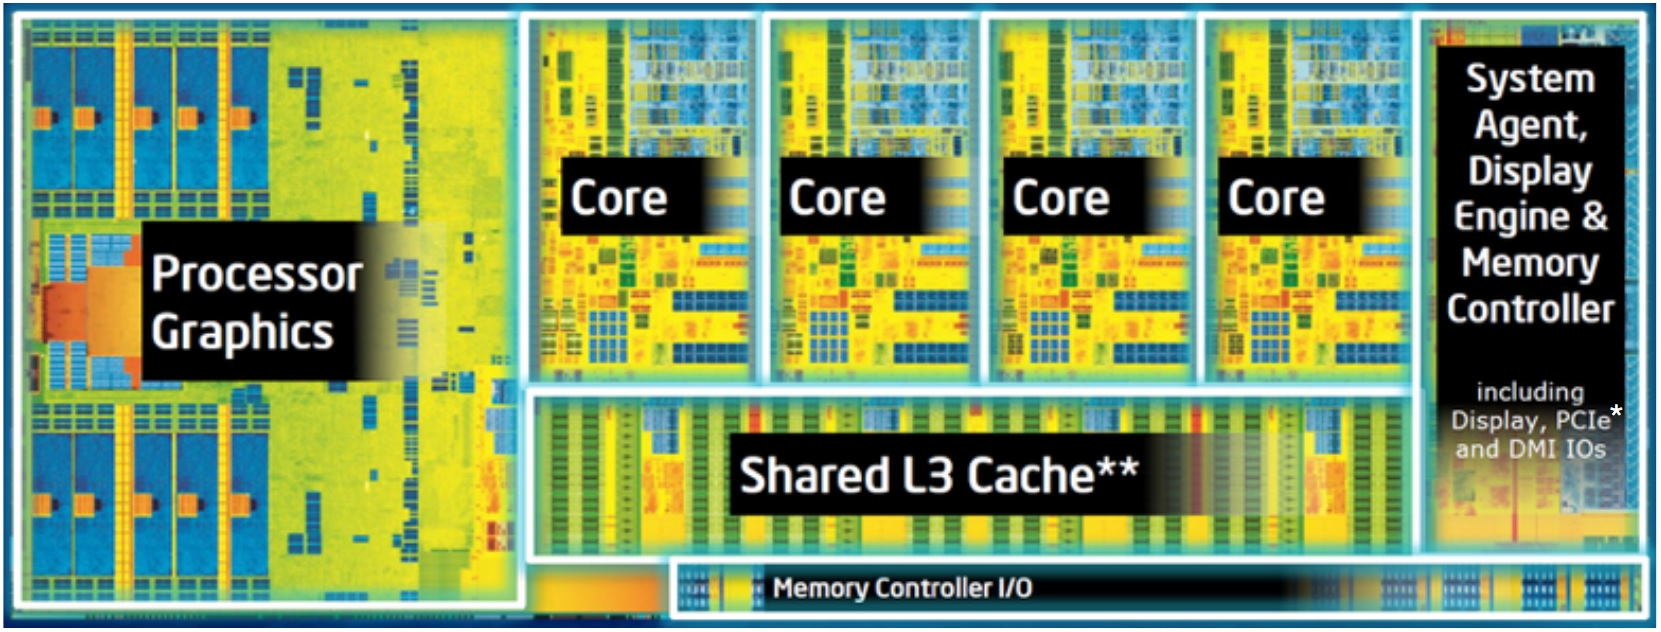
\includegraphics[width=1\textwidth]{background/graphics/i7intel.jpg}
 \caption{Intel Core i7 processor internal die photograph taken from intel whitepaper}\label{fig:i7}
\end{figure}
 
Chip Multicore Processors (CMPs) have become ubiquitous due to the difficulty in scaling single core performance.
In a CMP, multiple processor cores are put on a single package as can be seen in Figure~\ref{fig:i7}.
The most common CMP uses homogeneous cores as they reduce the design complexity both from a hardware and software perspective~\cite{}.
Unlike single core systems, the performance improvement in CMPs come from running multiple tasks in parallel.
These tasks can either be different programs or multiple threads from the same program running on the multiple cores.
By defining speedup \textit{S} to be the original execution time of the program over the new execution time with \textit{n} processors and \textit{f} representing the fraction of the program which can be parallelised; Amdahl's Law states

\begin{equation}
S = \frac{1}{(1-f) + \frac{f}{n}}
\end{equation}\label{amdlaw}

thus, given an infinite number of processor cores~\cite{ekhout2010amdalh}

\begin{equation}
\lim_{n\to\infty} S = \frac{1}{(1-f)}
\end{equation}

This second equation demonstrates how, given any program, the speedup obtained by using a CMP will be limited to the fraction \textit{f} of parallel code found in the program itself.
As all the processor cores are homogeneous this will cause serial bottlenecks to severely reduce the potential speedup as no core is adapted to speedup such regions.
This implication has pushed research into finding ways of parallelising code to its fullest~\cite{}, however this may not always be possible~\cite{}.
Thus whilst CMPs have become a mainstain in processor design, the homogeneous model has its limits.

\section{Heterogeneous Chip Multicore Processors}

Heterogeneous Chip Multicore Processors (HCMPs) or Asymmetrical Chip Multicore Processors (ACMPs) bring a variety of cores onto a single package.
This may come in different forms, such as multi-instruction set architectures on the same system on chip (SoC)~\cite{}, to same ISA, different size cores on an SoC~\cite{}.
Unlike CMPs, the variety of cores on an HCMP attempt to provide a certain amount of hardware flexibility to the software.
This can be used to provide efficient tradeoffs between speedup and energy/power savings by having programs run on larger or smaller cores~\cite{}.

\begin{figure}[t]
 \center
 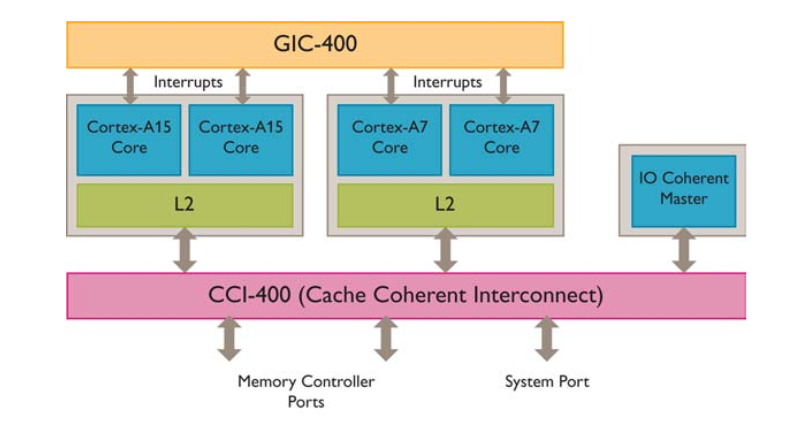
\includegraphics[width=1\textwidth]{background/graphics/biglittle.png}
 \caption{Example of a heterogeneous multicore processor proposed by ARM (big.LITTLE)}\label{fig:blarm}
\end{figure}


\section{Dynamic Multicore Processors}

% This section explains what a dynamic multicore is

In both CMPs and HCMPs, once the chip is fabricated the design cannot be modified, meaning that many of the trade-offs between power, performance and area cannot be changed after production.
Dynamic Multicore Processors (DMPs) attempt to bridge the gap between the two previous designs by allowing the execution substrate to adapt dynamically at runtime.
Mitall's survey ~\cite{MittalSurv2016} defines three types of modifiable resources: the core count~\cite{ipek2007CoreFusion}, number of resources that each core has~\cite{Homayoun3DPooling2012} and microarchitectural features~\cite{fallinhetblock2014,BauerRSE08,tavanaElastic}.
In this thesis I focus on DMPs that modify the core count.

Here, a DMP is composed of a group of homogeneous cores with a reconfigurable fabric.
The advantage of DMPs over the traditional CMP is the ability to reconfigure the processor to better match the tasks at hand.
For example, large sequential sections of code with high Instruction Level Parallelism (ILP) can be accelerated on a set of fused cores that mimic a wide superscalar processor.
On a parallel workload the DMP can be reconfigured by splitting the fused cores to match the Thread Level Parallelism (TLP).

\begin{figure}[t]
    \centering
    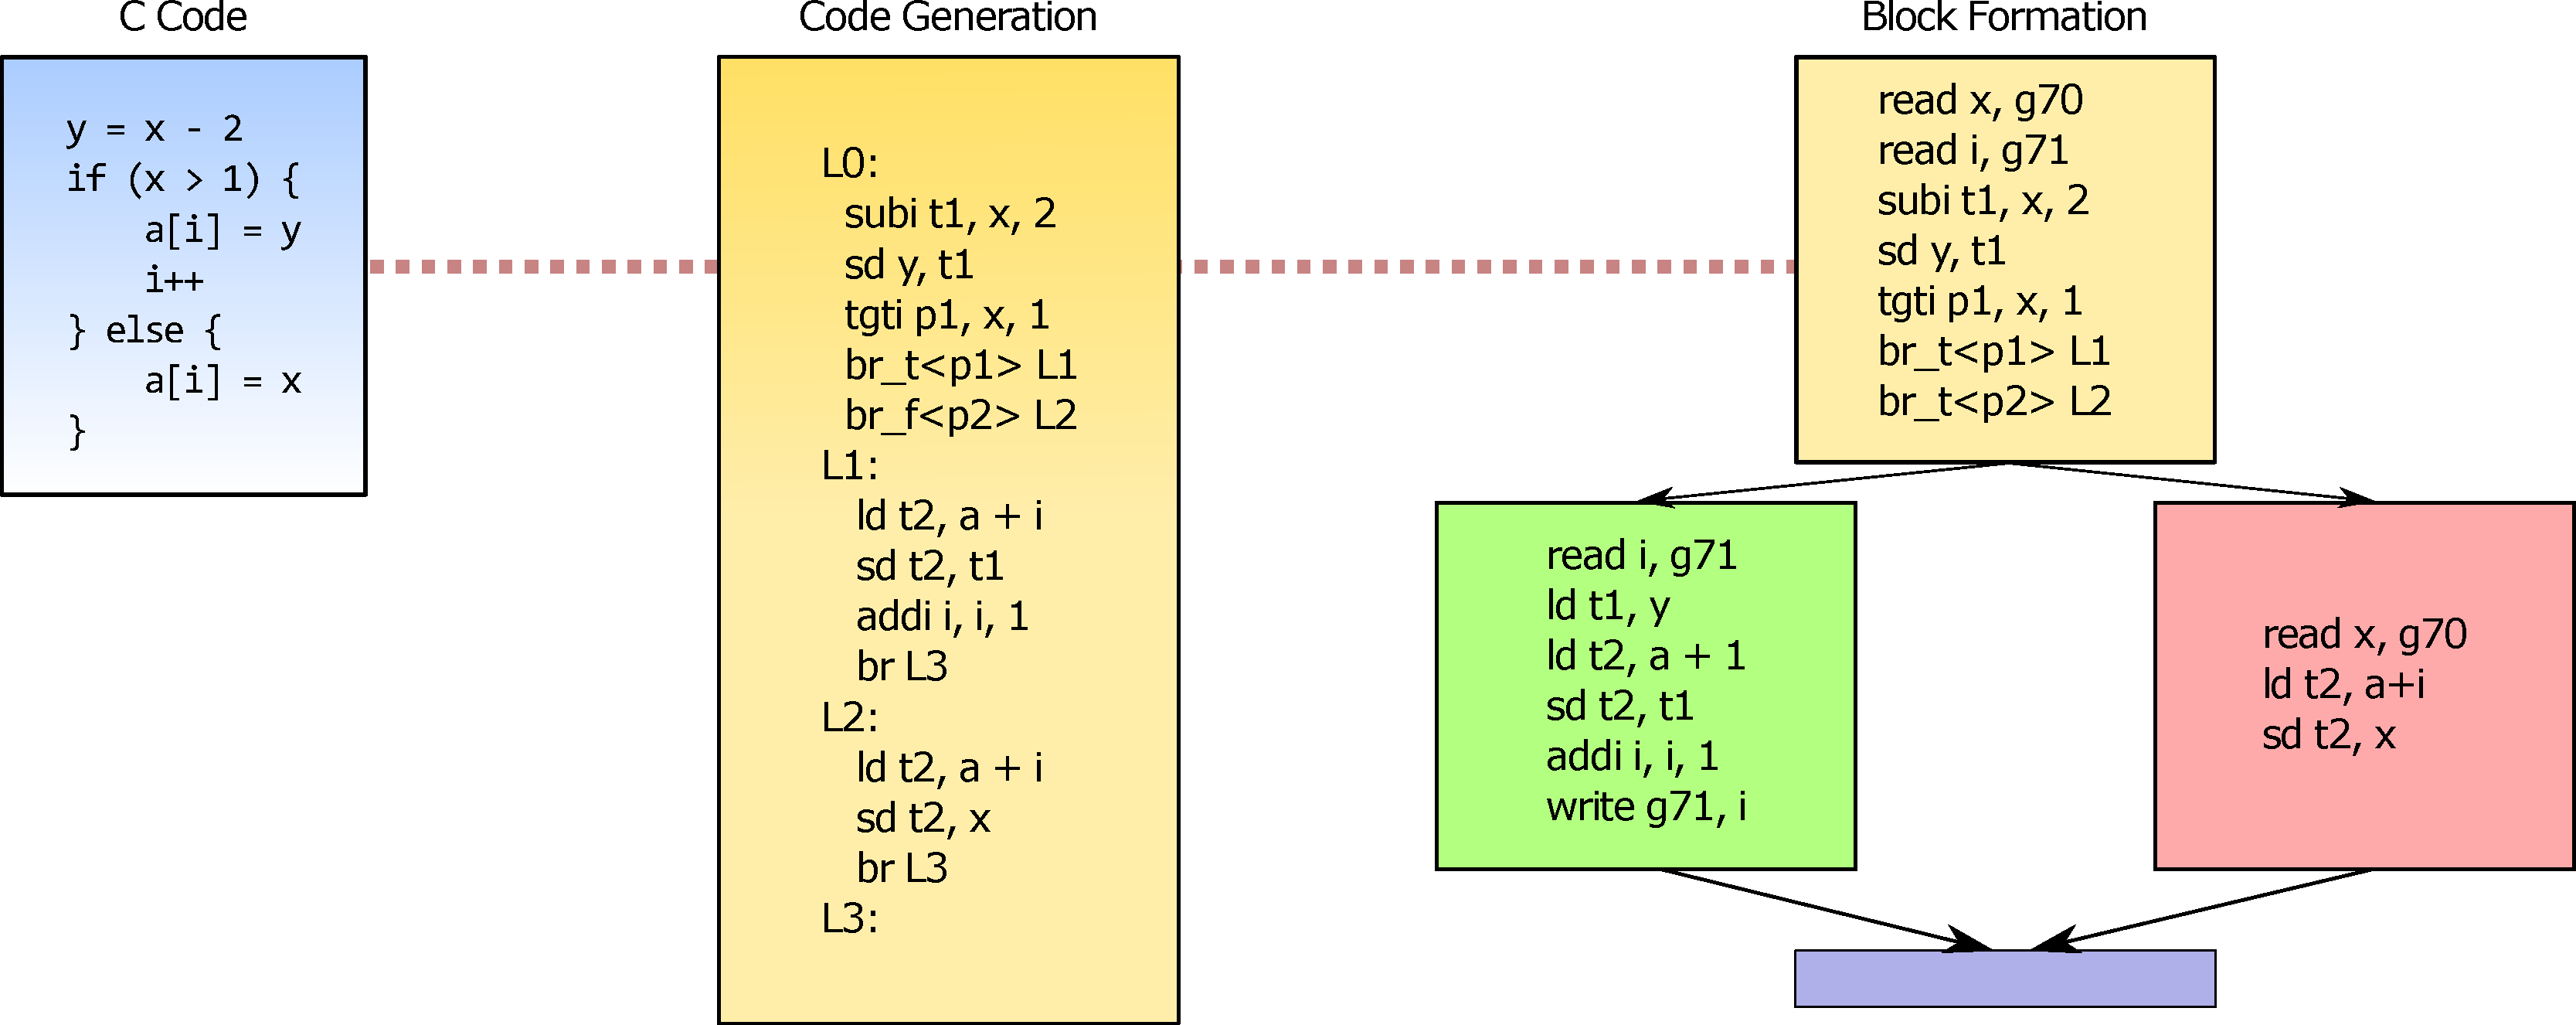
\includegraphics[width=1\textwidth]{background/graphics/EDGE_3.pdf}
    \caption{High-level view of the EDGE ISA flow.}
    \label{fig:EdgeHigh}
\end{figure}
\section{EDGE ISA} We assume a DMP similar to TFlex~\cite{kim2007tflex} using an Explicit Data Graph Execution~\cite{burger04edge} (EDGE) instruction set architecture (ISA).
EDGE ISAs encode dependencies between instructions at the ISA level.
Code is organised as blocks of instructions where all instruction communication is local to the block~\cite{smith2006edge}.
Each block has a single entry point but may have multiple exits.
This enables the architecture to dispatch blocks speculatively, with low overhead~\cite{putnam2010e2,kim2007tflex}, therefore, increasing exploitation of ILP.

\subsection{Core Fusion}
 \begin{figure}[t]
 \center
 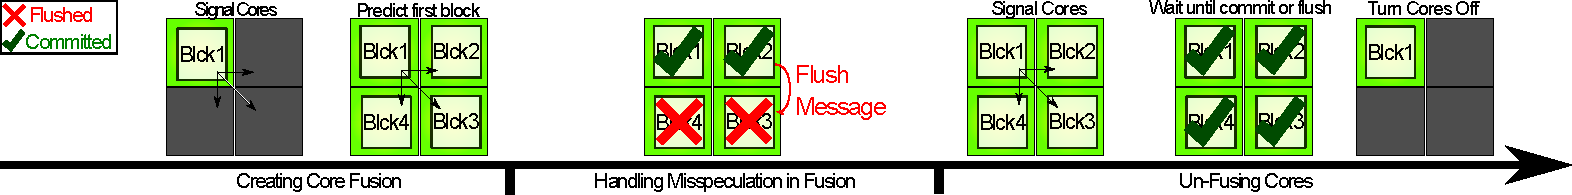
\includegraphics[width=1\textwidth]{cases-paper/graphics/background/proc_test.pdf}
 \caption{Core Fusion Mechanisms for our EDGE-based architecture.}\label{fig:dmp}
 \end{figure}
 
Core Fusion is achieved by fusing a set of \textit{physical} cores to create larger \textit{logical} cores.
This does not modify the physical structure of the chip, instead it provides a unified view of a group of physical cores to the software.
For example, fusing two cores generates a logical core with twice the amount of execution units, register files and L1 cache.
Fusion is a dynamic modification and may occur during the execution of a program to better fit the workload.
Unlike traditional CMPs, fused cores will operate on the same thread and attempt to extract Instruction Level Parallelism (ILP) rather than Thread Level Parallelism (TLP)~\cite{micolet2016dmpstream,pricopi2012bahurupi}.
Figure~\ref{fig:dmp} shows the different stages and mechanisms of core fusion for a four core system.
When creating a new core fusion a master core informs all other cores about the fusion and sends the predicted next block address to the next available fused core.
When a core mispredicts a branch in a fusion, it informs the other cores which flush any younger blocks.
When un-fusing, the master core informs the other cores, which then commit or flush their blocks and power down while the master core continues to fetch and execute blocks from the thread.
The extra hardware required to support dynamic reconfiguration is very minimal~\cite{kim2007tflex} since most of the machinery already in place can be reused such as the cache coherence protocol when fusing and un-fusing the cores.
We discuss this in further detail in Section~\ref{sec:setup}.

%\begin{figure}[t]
%    \centering
%    \includegraphics[width=.7\textwidth]{streamit-paper/graphics/dmcgraph.pdf}
%    \caption{High-level view of a dynamic multicore processor considered in this paper.}
%    \label{fig:dynmulticore}
%\end{figure}

%Explain the figure
%In this paper we consider a dynamic multicore processor which allows cores to compose their execution resources, register files and private L1 caches to create logical processors to accelerate a single thread.
%Figure~\ref{fig:dynmulticore} shows a high-level view of the architecture and the two possible states: composed and decomposed.
%The composed state represents a set of physical cores fused to create a larger logical core.
%Multiple sets of cores can be fused to create logical cores of different sizes.
%In Figure~\ref{fig:dynmulticore} for example, LP1 is composed of four physical cores whereas LP2 is composed of two.
%At runtime, physical cores may be decomposed from a logical processor to remove them from the core composition.

\section{Streaming Programming Languages}

% % This section should explain what steaming programming is (remove all the details about each language)
% General purpose programming languages often propose very little support for programs that handle with a continuous flow of data.
% This results in having to design a set of complicated for loops to manage the streams of data.
% Having to deal with different rates of incoming and outcoming data also increases the complexity of writing these applications using a standard language.

Streaming programming languages are a branch of dataflow programming that focus on applications that deal with a constant stream of data.
These applications, such as audio or video decoding can be commonly found in mobile devices.
Unlike conventional programming languages such as C++, these languages abstract the concept of incoming and outgoing data to permit the programmer to focus on how the data should be treated.
Programs are described as directed graphs where nodes are functions and their edges represent their input and output streams. 
These languages offer primitives to describe such a graph~\cite{theis2002streamit} which expose parallelizable and serial sections of the application directly to the compiler. 
Rates of incoming and outcoming data can also be defined to facilitate load balancing optimizations~\cite{chen2005rawstream}.

Features of streaming programming languages make them an ideal language for targeting multicore processors.
The explicit data communication between the different tasks in the program, the ability to estimate the amount of work performed in each task and information about data rates between tasks allows the compiler to easily generate a multi-threaded application that can run on a dynamic multicore processor.
However, the main challenge consists of deciding how to map the different tasks onto threads and how to allocate the right amount of resources to maximize performance.

\label{chp:bg}
\chapter{Related Work}~\label{chp:rw}
Whilst dynamic multi-core processors (DMPs) are relatively new in terms of processor design they are still a solution to a well researched set of problems.
These problems include improving performance of single-threaded applications and reducing energy consumption.
This chapter covers the related work relevant and adjacent to this thesis.
\vspace{-3em}
\section{Reconfigurable Processors}

This section covers work on both dynamic multi-core processors (DMP) and processors that can reconfigure their micro-architectures.
\vspace{-1em}
\subsection{Dynamic Multi-core Processors}~\label{chp:rw:sec:dmp}
The idea of composing physical cores was first introduced by Ipek {\it et.~al} in CoreFusion~\cite{ipek2007CoreFusion}.
CoreFusion employs a traditional architecture with 2 issue out of order cores.
When cores are fused, they collectively fetch from the same thread, whenever an instruction cache miss issued, an eight word block is delivered and distributed across in all of the cores' caches.
Fetches are aligned with the core responsible for the 2 oldest instructions.
In the original paper, a 4 core composition obtains a 1.3x speedup on SPEC 2000 INT and a 1.5x speedup on SPEC FP over a 2 issue core.
 
The Bahurupi~\cite{pricopi2012bahurupi} polymorphic heterogeneous multi-core architecture proposed by Pricopi {\it et.~al} introduces a sentinel instruction which informs the hardware about the \textit{live-in} and \textit{live-out} registers of a basic block.
Baharupi uses the SimpleScalar Portable ISA (PISA)~\cite{burger1997simplescalar}, and the compiler adds this instruction to the top of every basic block, splitting the program up into blocks similarly to EDGE.
They show that, on average this introduces a 24\% code size increase for SPEC 2006 INT, 15\% for SPEC FP and 19\% for Mediabench~\cite{mediabench} and MiBench~\cite{mibench} benchmarks.

Another important piece of information contained in this instruction is the size of a block.
Cores in a composition fetch basic blocks in a similar fashion to the one described in Chapter~\ref{chp:Background} Section~\ref{chp:Background:sec:EDGE}.
However, cores must execute global register renaming in the sequential order of blocks.
To ensure sequential renaming, a Global Program Counter (GPC) is introduced, and each core in the composition must lock the GPC before fetching a block and doing the renaming.
Using a 4 core composition they report a performance improvement of 2x on SPEC 2006 INT, 3x on SPEC FP and 4x on Mibench/Mediabench compared to a 2 issue core. 

TFlex~\cite{kim2007tflex} proposed by Kim {\it et.~al} is an EDGE processor that also deploys core composition.
They motivate that EDGE simplifies distributing instructions across cores as EDGE itself is designed for distributed micro-architectures.
Since instruction dependency orders are determined at compile time and encoded at the ISA level, the TFlex instruction fetching can be decentralised, as there is no need for centralised analysis like in a traditional ISA (such as register renaming or instruction number assignment).
Unlike the model used throughout this thesis, a block's instructions can be distributed amongst the cores in the composition, with one of the cores being the block owner.
As each core can be responsible for a single block, the total number of blocks in flight is equal to the number of cores in the composition.
In their work~\cite{kim2007tflex} Kim {\it et.~al} show that a 32 core composition can outperforms a single TFlex core by 3x on a set of EEMBC benchmarks and SPEC2000 micro-benchmarks.

The E2 processor is another EDGE based processor that can dynamically compose its cores~\cite{putnam2010e2}.
Unlike TFlex, a block is only executed on the core that fetches it, its instructions are not distributed.
E2 introduces the concept of segmenting the instruction window into lanes, allowing cores to fetch multiple blocks.
This allows E2 to be more adaptable to different block sizes; if the compiler can only generate small blocks, a core can have multiple blocks in its instruction window executing in parallel.
For example, if an E2 core has four lanes, each able to fetch a block of up to 32 instructions, it will be able to execute four times as many blocks in parallel compared to a TFlex core when the program being executed is made of blocks smaller than 32 instructions.
This means E2 can potentially extract more instruction level parallelism (ILP) from each core in the composition than TFlex can at any point.

Watanabe {\it et.~al} propose a different type of dynamic multi-core processor, where cores share execution units ~\cite{Watanabe2010Widget}.
The Wisconsin Decoupled Grid Execution Tiles (WidGET) architecture's design is based on a sea of resources, where a core is composed of a simple Instruction Engine (IE) that can send instructions to a set of available in order Execution Units (EU).
This allows for fine-grained reconfiguration of the cores: depending on the available ILP, an IE can increase the number of EUs it needs if there's a high amount of ILP available, or inversely reduce it.
Watanabe {\it et.~al} compare the performance of their processor to that of an Intel Atom and Intel Xeon using the SPEC2006 benchmark suite.
They show that using in-order cores with a fine-grained reconfiguration can reduce power consumption by 21\% compared to the Xeon whilst achieving the same performance.
It is even able to outperform it by 26\% whilst still reducing power consumption by 6\%.

\vspace{-1em}
\subsection{Reconfigurable micro-architectures}

MorphCore~\cite{khubaibMorphCore2012} focuses on reconfiguring a core for thread level parallelism.
It switches between out-of-order (OoO) when running single threaded applications and an in-order core optimised for simultaneous multi threading (SMT) workloads.
This provides an opposite solution to our DMP: providing a large core made for ILP that can be modified to better fit TLP workloads.
MorphCore outperform a 2-Way SMT OoO core by 10\% whilst being 22\% more efficient.

ElasticCore~\cite{tavanaElastic} proposes a morphable core that uses dynamic voltage and frequency scaling (DVFS) and micro-architectural modifications such as instruction bandwidth and capacity to adapt the processor to current needs.
Unlike heterogeneous systems that can present different sized cores on a single package, the ElasticCore is a single core with four different size configurations.
Each size configuration uses more resources than the previous, such as increasing the fetch width from 2 to 4 to 8 instructions.
Having all the resources on the single core allows adaptation to be quicker than migrating a thread to a  more appropriate core, 1000 cycles compared to the 10,000 for Arm's big.LITTLE architecture.

This similar to the work of Dubach {\it et.~al} \cite{dubach13dynamic} where micro-architectural features can be modified for better performance or energy efficiency.
They provide extensive analysis of SPEC 2000 benchmarks and demonstrate that machine learning and dynamic adaptation can double the energy/performance efficiency compared to a static configuration.

\paragraph*{Summary}
Whilst CoreFusion and Bahurupi use traditional ISAs, they must either support a limited version of composition where a single eight word block is distributed amongst cores (CoreFusion), or add extra instructions which increase code block size by up to 24\% (Bahurupi).
In the EDGE architecture, instructions are naturally formed into blocks, and instructions in a block do not communicate via registers; this simplifies the fetching of multiple blocks.
Thus TFlex does not need a centralised structure for fetching instructions~\cite{kim2007tflex}, however, it does not support the ability of fetching multiple blocks on a single core.
Instead, each core can fetch a single block and dispatch instructions on all other cores in the composition.
If blocks are small, then the instruction window of each core will never be filled, which in turn reduces the potential performance of core composition.
E2 addresses this problem by segmenting the instruction window into separate lanes and allowing each core to fetch multiple blocks.
This makes it more flexible than TFlex as each core will have more instructions to execute on average, allowing each core to extract more ILP.
Thus, the processor used in this thesis based on the E2.

\section{Automated processor reconfiguration}

In Ipek {\it et.~al}'s. original work on CoreFusion~\cite{ipek2007CoreFusion} they introduce the \textit{FUSE}/\textit{SPLIT} instructions that allow for dynamic reconfiguration.
However, their eight core system only has two possible configurations: either each core executes on their own or they are fused into groups of four cores; no details as to when to compose cores is discussed.
This the same for the original proposal for TFlex~\cite{kim2007tflex}, where 5 different configurations are explored (2, 4, 8, 16 and 32 composed cores), but does not provide any insight as to how to determine the composition size automatically.

In the work of Pricopi {\it et.~al}~\cite{pricopiSchedCoreComp2014}, they show how dynamic reconfiguration is beneficial when it comes to scheduling multiple tasks.
However, they do not discuss any method of automatically deciding the optimal configuration beyond a 4 core composition.
In their work they use speedup functions determined from profile executions of applications to determine how to schedule tasks.
This means that whenever an application is modified, it must be re-analysed to benefit from dynamic composition.
They do not discuss what software characteristics help determine when to reconfigure the cores, or how to optimise software.

Gulati {\it et.~al} propose an offline and online scheduling algorithms for TFlex \cite{gulati2008multitaskingdmc}. 
This work focuses on maximising speedup for a set of workloads in a multi-tasking environment.
The offline model first profiles a program on different compositions and then uses that information to make a decision at runtime whilst their online model simply changes the size of the current composition by +/-1 core and then evaluates whether or not that modification improved performance.
In their results they show that the offline profiling tool outperforms the online algorithm.
As the threshold is set ahead of time, the online model is not able to fully utilise the system when applications do not meet the required threshold.
They demonstrate that a DMP that can adapt to workloads can result in faster response times than a tradition CMP, between 21\% to 13x faster.

\paragraph*{Summary}
The main contributions in automatic reconfiguration rely on profiling information to make a decision.
This means that new applications will need to be executed multiple times in order to generate a profiling information used by the DMP to decide when and how to reconfigure itself.
This procedure can be costly if the number of ways the processor can be reconfigured is high (for example when a programmer must choose between multi-threading and core composition).
Whilst Gulati {\it et.~al} propose a runtime solution~\cite{gulati2008multitaskingdmc}, this does not \textit{directly} infer a correct composition, instead it changes the composition size by +/- 1 at each reconfiguration interval.
They admit that this system is less efficient than profiling.

These contributions lack the ability of determining a how to configure the DMP without the use of profiling information.
If a model that can predict how the DMP should be configured to maximise either speedup or energy efficiency without requiring multiple executions of the program, then this would make using DMPs easier.
This why this thesis examines how machine learning can be used to reconfigure the DMP.
Machine learning can be used to generate models that \textit{learn} from how programs are affected by core composition to determine the correct configuration of the DMP for any new program.
Through this method, the procedure of finding a good configuration can be reduced to a single analysis of the application at hand.

\section{Code optimisation for EDGE}

Whilst there exists no literature on code optimisations geared towards improving the performance of core compositions, some previous work exists on studying how block sizes affect the performance of the EDGE architecture.
Smith {\it et.~al} highlight the importance of block size in their work~\cite{smith2006edge}, stating that larger blocks will lead to better performance.
They suggest the use of instruction predication~\cite{smith2006dataflowpred} that allows EDGE blocks to be fused into a single block, called a hyperblock.

Since EDGE instructions pass their results directly to an instruction's input operands, some optimisations are required to ensure that predicates are efficiently broadcast to all depending instructions.
The optimisations are predicate fanout reduction, path-sensitive predicate removal and instruction merging~\cite{smith2006dataflowpred}.
Overall, hyperblocks are able to improve the performance of a set of EEMBC benchmarks by 29\% compared to only using basic blocks.
Using the optimisations previously defined improves the performance of hyperblocks by up to 12\% compared to non-optimised hyperblocks.
\vspace{-1em}
\section{Improving instruction fetching for composition}
Fetching instructions on core compositions can be a challenge, as will be discussed in Chapter~\ref{chp:hardchanges}.
This section covers how this issue has been address in previous research.

Robatmili {\it et.~al}~\cite{robatmili2011uniproc} discuss how to improve block fetching for the TFlex processor by selectively refreshing blocks.
A block refresh involves keeping the block in the instruction window and flushing the buffer operands and then re-executing the block, skipping the re-fetch.
First, they modify TFlex so that blocks are executed locally on the core instead of dispersing the instructions of a block on multiple cores.
The two main assumptions made are that a core can only ever execute a single block at a time, and once the block is committed, it can remain in the instruction window.
When a new block request is made, the coordinator core in charge of the new block checks to see if any inactive core has that block stored in their window.
If it does, then that core is activated and starts re-executing the buffered block.
If no idle core has the block in their window, then the coordinator core will ask one of those cores to fetch the block and start executing it.
They show that cores may have to store up to 8 blocks in the instruction window to ensure that 75\% of the total executed blocks come from a refresh.
Overall this technique can improve the performance of a 16 core composition on a set of SPEC 2000 benchmarks by 1.08x on average, with a maximum speedup of 1.16x.

This implementation depends on the concept that cores in the composition currently hold inactive blocks in their instruction window.
Whilst this may be the case for TFlex, as it can only execute a single block per core, an E2 type processor is designed to not have idle blocks in its composition.
Therefore, another solution to improve fetching for the type of processor used in this thesis proposed in Chapter~\ref{chp:hardchanges}.

\vspace{-1em}
\section{Hardware techniques for power and energy efficiency}

Chapter~\ref{chp:cases} focuses on changing the size of a core composition at runtime to the energy consumption of single threaded applications whilst still maintaining the same execution times as the fastest static core compositions.
This section covers the different techniques for reducing energy consumption using hardware techniques.

\subsection{Dynamic Voltage and Frequency Scaling}
Dynamic Voltage and Frequency scaling (DVFS) is a method of modifying the power and energy consumption~\cite{paganiEECHM2017} by modifying the voltage or the clock rate of the processor.
Often times, DVFS is used to reduce energy or power consumption in phases of low performance.

Herbert {\it et.~al} in ~\cite{herbertDVFS07} demonstrate that DVFS is an effective technique for reducing $energy/throughput^2$ ($E/T^2$).
They suggest two methods of using DVFS: controlling it at a per-core basis, or at a cluster basis, also known as Voltage Frequency Islands (VFI).
Using VFIs reduces the design complexity of both the hardware and algorithms that control DVFS.
They demonstrate that on a 16 chip multi-core processor (CMP), DVFS can reduce $E/T^2$ by 38.2\% on a set of multi-threaded workloads.
The results also highlight how core-level DVFS does not reduce $E/T^2$ significantly compared to using VFIs: 38.2\% for core-level, compared to 37.9\% for a 4 core VFI.

Pagani {\it et.~al} consider the use of VFIs in a heterogeneous system in ~\cite{paganiEECHM2017}, where cores in a VFI are homogeneous, but the different VFIs are heterogeneous.
Their objective is to ensure that tasks are running on the most energy efficient core whilst satisfying the time constraints of the task.
Once a task is partitioned and dispatched onto a core in a VFI cluster, Pagani {\it et.~al} use Single Frequency Approximation (SFA)~\cite{sfaScheme} as the DVFS strategy.
SFA determines a single voltage/frequency that satisfies timing constrains of a task.
This technique results in an average reduction of energy consumption of 25\% and still ensures all tasks finish on time.


Vega {\it et.~al} ~\cite{vega2013crank} underline that whilst DVFS is an effective way of reducing power and energy consumption, the fact that it is decoupled from other techniques such as per core power-gating (PCPG) reduces the overall benefits.
They suggest an online algorithm at the OS level that collects data from performance counters and makes multiple decisions based on the data gathered.
%write more
%However this approach is orthogonal to DMPs~\cite{sibi2014}, whilst both techniques (DVFS and core composition) adapt to programs phases, DMPs can also be used to speed up the execution of programs.
\vspace{-1em}
\subsection{Thread migration in HCMPs}
Arm big.LITTLE~\cite{armbig} is an example of a heterogeneous chip multi-core processor (HCMP) that provides two different types of cores to allow the programmer to choose between energy efficiency and performance.
A program can be migrated from one core to another depending on the requirements, however this comes at the cost of a very high migration overhead, over 10,000 cycles~\cite{armbig}.
However Gutpa {\it et.~al} show that by selecting the correct core configuration at runtime this can lead to an energy reduction of up to 46\%

%More on HAQUE
Haque {\it et.~al} show that an HCMP is able to reduce energy consumption and improve throughput for applications with high-percentile latencies~\cite{tailAMP2017}.
They highlight that service providers receive requests of different lengths of computation.
By successfully scheduling the different lengths to the correct cores in an HCMP, they can reduce the energy consumption of short requests by a factor of 50\% compared to DVFS.

Adileh {\it et.~al} argue that current proposals for scheduling tasks on small or large cores are inadequate when operating on a power-constrained HCMPs in a multi-tasking environment~\cite{adileh2016power}.
Using linear programming they determine that applications can be ranked based on their delta performance/delta power (DPDP) which is defined as the ratio of performance and power difference between executing an application on a small or large core.
Applications that ranked highly are executed on the large core whilst others are executed on the smaller cores.
After defining five schemes that used DPDP to schedule tasks within a power budget of 1W per second per application they show that it outperforms other schemes by 16\% on average and up to 40\%.
 
Gupta {\it et.~al} tackle the issue of the high number of configurations possible in an HCMP by characterising workloads offline~\cite{Gupta2017Dypo}.
Applications are executed and their performance is recorded on the different available cores, with different parameters tuned such as the core's clock frequency.
Then, for different optimisation goals they found the Pareto-optimal configuration for each of the benchmarks.
This information is then used to build a classifier that can determine the correct core configuration for a given snippet of an application.
Using this classifier Gupta {\it et.~al} are able to improve performance per watt of a set of single and multi-threaded benchmarks by 93\%, 81\% and 6\% compared to an interactive, on demand and powersave governor respectively.

\paragraph*{Summary}
These different techniques show that either dynamically changing some parameters of the hardware (DVFS) or moving where a program is executing (thread migration) is an effective way of reducing energy consumption.
However, all these techniques rely on fixed configurations of the processor, such as an HCMP where the core configurations are determined at design time. 
\vspace{-1em}
\section{Speculative Execution}
Core composition is able to improve the performance of applications by executing many instructions speculatively from the same thread.
This section covers work on speculative parallelism, where performance improvements are obtained by speculatively executing multiple tasks in parallel, rather than through deep branch prediction.

\paragraph*{Software level}
The idea of speculatively extracting parallelism at runtime was first introduced by Rauchwerger {\it et.~al}~\cite{runtimeSpec}.
They underline that compile-time analysis of single-threaded programs does not allow for the complete detection of parallel sections, and must be complemented by runtime analysis.
They propose a framework for parallelising loops at runtime: instead of detecting if the loop is parallelisable or not, the loop is speculatively executed in parallel and then runtime analysis conducted to verify that no data-dependencies are violated.
If any violations occur, the loop is re-executed serially.
Loops must be marked as speculatively parallel by the compiler, the run-time system only verifies whether or not the speculative execution violates dependencies.

Hertzberg {\it et.~al} push the idea of speculative multi-threading further in ~\cite{dbtspec2011} by using dynamic binary translation (DBT) to generate optimised parallel code on the fly, they name this the Runtime Automatic Speculative Parallelism technique (RASP).
Instead of generating speculative parallel loops at compile time, they propose that idle cores should be used to analyse running programs and generate parallel versions of the loops.
The code continues to be analysed even after the generation of parallel loops in order to ensure that the optimal code has been generated.
Using RASP, Hertzberg {\it et.~al} demonstrate that their system can lead to a performance increase average of 1.46x on SPEC2006 integer benchmarks and up to a 3x speedup on SPEC2006 floating point benchmarks compared to single-threaded execution.

Whilst the work proposed by Hertzberg {\it et.~al} motivates pairing DBT with speculative parallelism, Koch {\it et.~al} show in ~\cite{koch2013spec} that the majority of the speedup obtained arises from the DBT optimisations and not speculative parallelism.
As serial programs can also benefit from DBT optimisations, Koch {\it et.~al} argue that the work in Hertzberg {\it et.~al} does not necessarily motivate dynamic binary parallelisation (DBP) but instead DBT.
Without DBT, RASP only provides a 1.12x speedup on SPEC2006 integer benchmarks, compared to the 1.46x when DBT optimisations are turned on.
Koch {\it et.~al} underline that the cost of detecting loops which can be parallelised, paired with the cost of starting threads can often outweigh the performance benefits of DBP.
 
\paragraph*{Hardware level}
Jeffrey {\it et.~al} present a novel tiled architecture called Swarm~\cite{swarm2016} that performs aggressive thread-level speculation.
The Swarm architecture executes tasks that are identified via timestamps.
Each task can access any data and has the ability to generate new tasks, also known as children, that will be assigned a greater timestamp.
All tasks are maintained by a task-queue, and can be executed out of order.

Swarm is extended by Abeydeera {\it et.~al} their speculation aware multi-threading policy SAM~\cite{Abeydeera2017SpecMulti}.
According to Abeydeera {\it et.~al} having a high number of speculative threads often leads to a large number of aborted tasks which impacts performance.
SAM extends Swarm by ensuring that tasks with lower timestamps are prioritised as they are most likely to commit, thus reducing the number of aborted tasks.
This technique of determining which tasks to run is called issue stage prioritisation.
They also relax conflict resolution by using a similar technique to Wait-n-GoTM~\cite{waitNGo2013}.
Instead of assigning tie-breakers to tasks when they are spawned, SAM assigns them when a task acquires a dependence from another task with equal timestamp; this reduces the number of needless aborts.
Overall, an 8 in order core Swarm processor with SAM improves performance by 2.33x compared to a single core for a set of graph algorithms.

Subramian {\it et.~al} present a new execution model that supports nested parallelism and is implemented for a Swarm~\cite{fractal2017} .
Fractal introduces the concept of grouping tasks into hierarchies of nested \textit{domains}.
Tasks in a domain can either execute in order or out of order relative to their timestamps and appear to execute as a single atomic unit to other domains.
By allowing tasks to generate domains, Fractal is able to exploit nested parallelism without complicating the software, and can lead to a performance increase of up to 88x compared to Swarm on some graph algorithms.
\vspace{-1em}
\paragraph*{Summary}
This section has shown how an alternative form of speculation can be used to improve the performance of applications.
This supported both at the hardware and software level.
As seen throughout the section, speculative parallelism requires both hardware and software support to function (SWArm).
This is more involved than supporting core composition on an EDGE processor, where the ISA naturally lends itself to deep single-threaded execution speculation.
\vspace{-1em}
\section{Tackling data-dependencies}
This section covers the different techniques used to tackle data-dependencies that affect a processor's ability to extract instruction level parallelism, which is the main way core composition improves performance.
\subsection{Value Prediction}
Value prediction is a technique used to speculatively resolve data dependencies between instructions and is used in Chapter~\ref{chp:hardchanges}.
This section covers the different proposed techniques, including the one used in that chapter. 

The earliest work on value prediction can be retraced to Mikko {\it et.~al} where they propose a \textit{Load Value Predictor} \cite{lipasti96valpred} that predicts the value of load instructions.
They show that performance can be improved by up to 27\%.

Perais {\it et.~al} propose the VTAGE \textit{context} value predictor ~\cite{peraisVTAGE2014}, that adopts the same prediction scheme as the ITTAGE branch predictor~\cite{SeznecITTAGE}.
Using global branch history, which is easier to maintain that data-flow history~\cite{peraisVTAGE2014}, VTAGE can improve performance of some SPEC 2000 and 2006 applications by up to 65\%.

The block based D-VTAGE predictor~\cite{peraisBeBop2015} can quickly issue multiple predictions grouping up predictions as a single block.
The basic prediction fetch and update mechanism are inherited from VTAGE, except D-VTAGE is a \textit{computational} value predictor.
In order to improve value prediction for tightly knit loops where multiple iterations of the loop body can be live in parallel, the predictor employs a speculative window that is able to keep track of live speculative data.
D-VTAGE is able to obtain up to a 1.7x speedup, and averages a 1.10x speedup on a set of SPEC 2000 and 2006 applications. 

Miguel {\it et.~al} propose a different technique for value prediction called load value approximation \cite{miguel2014LoadVal} for applications where value inexactness is acceptable.
Applications such as image tracking or image comparison do not need to operate on exact values as they often allow for a margin of error.
Therefore, these applications do not need to roll-back on a mispredicted value, and can continue to operate with incorrect data as long as it is sufficiently accurate (an error rate below 10\%).

Sheikh {\it et.~al} present a value predictor that is able to avoid mispredictions caused by Load $\,\to\,$ Store $\,\to\,$ Load conflicts~\cite{sheikh2017value}.
This achieved by predicting load memory address at the instruction fetch stage and checking the data cache for that memory address.
If the memory address is contained in the data cache, then the value is fetched (this considered a prediction).
If the address is not contained in the cache, then a data prefetch issued.
Their new approach to value prediction generates a 4.8\% speedup on a set of SPEC 2000 and 2006, EEMBC and Octane applications.
This almost 2x more than the VTAGE predictor used in the paper (2.1\%).

\paragraph*{Summary}
Most of the predictors described in this section focus on value prediction for load instructions.
Whilst loads can be slow to execute causing longer data-dependency stalls, the EDGE architecture's reliance on registers for intra-block communication is also a prime suspect.
Overall, the D-VTAGE predictor is the most adequate solution for this thesis, as will be explained in greater detail in Chapter~\ref{chp:hardchanges} Section~\ref{chp3:sec:val}.

\subsection{Data Prefetching}
Whilst value prediction is used to mask data dependencies or long latencies caused by cache misses by predicting values, data prefetching attempts to make data available in L1 caches before it is needed.
This can be achieved both in software by inserting instructions that trigger a data fetch-request ahead of time, or in hardware by analysing memory access patterns.

Ainsworth {\it et.~al} ~\cite{graphPrefetch2016} suggest that a stride-based prefetcher is not adequate for irregular memory accesses.
They propose a hardware prefetcher that has knowledge on the data structures being treated, to be able to trigger multiple prefetches based on loads snooped on the L1 cache.
Using Breadth-First-Search (BFS) as an example with the compressed sparse-row data format, they demonstrate that a specialised prefetcher can improve performance by a factor of 2.3x compared to stride prefetching and software prefetching that only generates a 1.1x speedup.

Prefetching for indirect memory accesses is considered difficult when using a hardware prefetcher~\cite{lee2012whenprefetchworks,prefetchForIndirect2017}.
Thus Ainsworth {\it et.~al} also propose a compiler pass that inserts non-blocking loads to enable prefetching for indirect memory accesses in ~\cite{prefetchForIndirect2017}.
The compiler pass targets loads inside loops whose addresses depend on a loop induction variable and meet a set of conditions to ensure that the prefetches do not cause faults.
Once the loads have been detected, the prefetches are scheduled based on a formula they devise in the paper.
The formula takes into account the number of loads found in the prefetch sequence for the loop, the position of the real load, and a constant that is based on architectural features such as memory latencies and the possible IPC.
Using their compiler pass they are able to improve the average performance of memory intensive benchmarks by 1.1x to 2.7x on different processors.
\vspace{-1em}
\subsection{Register Bypassing and Criticality Detection}
Whilst value prediction is used in Chapter~\ref{chp:hardchanges}, there exists previous work on trying to reduce the latencies caused by data-dependencies in core composition; this section describes the solution.

Robatmili {\it et.~al}~\cite{robatmili2011uniproc} discuss the potential bottlenecks caused by data-dependencies when executing blocks on large core compositions.
This work uses the TFlex processor and presents the Distributed Block Criticality Analyzer (DBCA) that can gather criticality information to optimise the execution of instructions at runtime.
The DBCA is able to detect and predict which instructions are late communication edges, that is the last register writes in a block that younger blocks depend on.
When a block is fetched, the core calls the DBCA to get the predicted registers to determine which register writes are late communication edges.
Once the values of these instructions are produced they are forwarded to the successive speculative block directly, bypassing the register file.
Using this techniques, Robatmili {\it et.~al} show that for a 16 core composition (TFlex processor), the performance of a set of integer SPEC 2000 benchmarks can be improved by 1.08x on average and up to 1.16x at best.

The reason this technique cannot improve performance much more is due to the fact that it only attempts to detect which instructions should use register bypassing.
This model can still involve significant latency, as the late communication edges may require data from previous instructions as well, increasing the critical path chain.

\vspace{-1em}
\paragraph*{Summary}
Data prefetching and register bypassing can help alleviate the effect of data-dependencies by ensuring that data-dependent values arrive quicker to their destination.
Unlike value predictors, data prefetching is a technique that is actually implemented in both compilers and real commercial processors~\cite{intelmanual}.
Yet both data prefetching and register bypassing do not allow for instructions to execute with speculative data, which, as will be seen in Chapter~\ref{chp:hardchanges} is better for increasing ILP in large core compositions.
\vspace{-1em}
\section{Dataflow Programming Languages}

Chapter~\ref{chp:streamit} explores how a DMP can be used to improve the performance of applications written in a dataflow programming language.
This section describes a set of data flow programming languages and what hardware they target.

StreamIt~\cite{theis2002streamit} is one of the first programming languages directed towards streaming applications.
As previously described in Chapter~\ref{chp:Background} Section~\ref{sec:bg:stream}, StreamIt defines a set of constructs to build scalable parallel streaming applications.
StreamIt was originally intended for the RAW~\cite{waingold1997raw} tile-based architecture, but can be used in other settings as well.

Brook~\cite{buck2004brook} is another streaming programming language geared towards Graphical Processing Units (GPUs).
Unlike StreamIt, Brook extends the C language by providing a new data type and function types.
The new data type, called a \textit{stream}, provides a collection of data which can be operated on in parallel, which can be modified by stream functions.
A stream function takes one or more stream inputs and will output one or more streams; this similar to a StreamIt \textit{filter}.
To operate on streams in parallel, Brook defines a subset of stream functions called \textit{kernel} functions.
These functions do not have access to global values, cannot call functions that aren't kernel functions as well, and are only allowed to access streams in a read-only \textit{OR} write-only way.
This to facilitate the compiler generation of dataflow graphs for the program.

WaveScript on the other hand is developed for embedded systems that are low powered \cite{newton2008wavescript}.
Unlike StreamIt, WaveScript uses an asynchronous streaming model, where the input and output rates of functions are not known at compile time.
%Programs are not defined as graphs, instead 

Bosboom {\it et.~al} demonstrate how a streaming language can be directly embedded into a more common host-language in ~\cite{bosboom2014streamjit}.
They present StreamJIT which inherits StreamIt's programming structure, however the language is embedded inside Java.
This allows the new StreamJIT language to benefit from the front-end compiler optimisations developed for Java; a method they call \textit{commensal} compilation.
\vspace{-1em}
\paragraph*{Summary}
Brook and WaveScript are both domain specific languages for architectures not explored in this thesis (low powered embedded systems and GPUs).
As StreamIt is used to construct scalable parallel streaming applications it makes it a perfect candidate for exploring how to partition multi-threaded applications on a DMP, as seen in chapter~\ref{chp:streamit}.
Since the current system used does not have a Java Virtual Machine (JVM) it cannot support the commensal compilation technique described by Bosboom {\it et.~al}.

\section{Partitioning streaming programs on multi-core chip}
Chapter~\ref{chp:streamit} explores how partitioning streaming applications on a DMP improves performance.
This involves determining which number of threads leads to the best execution time, and how many cores each thread needs.
This section covers work on partitioning streaming applications. 

Previous work on scheduling streaming applications focuses on finding mathematical ways of partitioning the graph onto the chip ~\cite{carpenter2009streammap,kudlur2008orchestratingstreamprog}.  
In Carpenter {\it et.~al}'s work~\cite{carpenter2009streammap} they restrain themselves to partitioning a StreamIt application maintaining correctness.
Correctness can be defined as a subgraph where the filters are connected. 
This restriction reduces the number of potential partitions that can be generated by their algorithm and will put TLP in favour of ILP. 

Kudlur {\it et.~al}~\cite{kudlur2008orchestratingstreamprog} choose to represent the partitioning problem as an integer linear programming problem.
They start by fissioning stateless filters to obtain the optimal load balance across all cores and assign the filters to a core using a modulo scheduler.
Farhad {\it et.~al} also use integer linear programming in~\cite{farhad2012streamilp} to schedule StreamIt programs on multi-core.
They profile the communication costs of the streaming programs by running the program using different multi-core allocations and feed that information into their integer linear programming model.

Using a machine learning model to partition StreamIt programs was previously explored in the work of Wang {\it et.~al} ~\cite{wang2013partitionstreamit}.
They use a k nearest neighbour (kNN) model to determine the perfect partitioning of a StreamIt program for a multi-core system. 
Their model is used to find ways of fusing and fissioning filters to discover a new graph that can then be mapped onto a multi-core system.
\vspace{-1em}
\paragraph*{Summary}
Whilst this previous work focuses on determining a partition of streaming applications through mathematical models or integer linear programming, Wang {\it et.~al} ~\cite{wang2013partitionstreamit} show that machine learning can be used.
However, none of these proposals explore DMPs, instead focusing on processors with fixed designs.
This means that whilst some techniques such as kNN can be used to automate the partitioning decision, there still lacks any exploration of how the thread/core composition design space affects the performance of streaming applications.
This thesis therefore conducts that exploration to generate a new model for partitioning streaming applications on DMPs.
 

\section{Machine-learning guided performance optimisations}

Using machine learning to increase performance has been a popular area of research as of late.
There are two areas in which machine learning is used: compiler driven optimisations and runtime driven optimisations.

Dubach {\it et.~al} use machine learning to determine what the performance and energy consumption will be based on the micro-architectural parameters and compiler optimisations that are used in ~\cite{DubachExpl2012}.
Their work explores the 35 MiBench benchmarks by modifying compiler optimisations and micro-architectural features of an embedded system.
Over 1000 compiler flags are explored, and 200 configurations of the processor are used (modifying cache sizes, associativity, branch target buffer sizes and associativity).
Their design space exploration shows that to obtain the best performance for each of the applications, both the compiler optimisations and processor must be tuned.
They then use this information to build a machine learning model using an Artificial Neural Network which is able to predict the performance, in terms of $Energy \times Delay \times Delay$ of an application given a set of compiler flags and micro-architectural features.
Their model is able to predict a performance that is close to the best in the space with an error rate of just 3.2\%.

Cummins {\it et.~al} developed a deep learning model that takes source-code and is able to learn how the code correlates to performance~\cite{cummins2017pact}.
Their deep learning model ingests source-code and through a set of transformations, and through training the model, it is able to also generate optimisation heuristics.
They train their deep learning model for two scenarios: GPU thread-coarsening and CPU/GPU task partitioning.
Compared to state of the art hand-crafted heuristics, the deep learning model is able to outperform both scenarios by 12\% and 14\% respectively.
\vspace{-1.5em}
\section{Summary}
This chapter underlined that encoding instruction dependency order at the ISA level makes EDGE a more attractive architecture for core composition~\cite{kim2007tflex}.
It then showed that of the two EDGE based architectures discussed, the fact that E2 can support a higher number of blocks that TFlex in a composition makes it more interesting, as a higher block count means more ILP can be exploited.
The E2 processor is therefore used as a base in this thesis.

Then the different techniques for automatically configuring a DMP were explained.
Overall, they rely on profiling applications in order to make decisions meaning that multiple executions of a program are required to create a profile that is used to configure the processor later on.
This can be an expensive procedure if the number of configurations is large.
This thesis tackles this issue by presenting models that use machine learning to determine the correct configuration of the DMP without requiring multiple executions of the program; making DMPs more practical to use.

This was followed by explaining how block fetching latencies can be reduced to improve the performance of core composition.
This work was conducted on a TFlex processor and depends on idle-cores to selectively re-issue blocks on idle cores.
Whilst this a promising approach for a TFlex processor, E2 avoids having idle cores by allowing them to fetch multiple blocks, and thus the concept of instruction buffering is not applicable.

This was followed by exploring different hardware techniques used to reduce the energy consumption of applications, which is a topic approached in Chapter~\ref{chp:cases}.
These techniques (DVFS and thread migration) often rely on the processor cores to be designed ahead of time to create performance models, and they can sacrifice some speed to reduce energy consumption.
This thesis will show how a DMP can be dynamically reconfigured to reduce energy consumption whilst obtaining the best execution time of a static composition.

Another method of speculative execution was then described: hardware and software techniques that exploit thread-level speculation.
These techniques are described to show the breadth of performance optimisations via speculative execution.

Value prediction, data-prefetching and register bypassing were shown to be methods of reducing the impact of data-dependencies between instructions.
Even though data-prefetching is successfully applied in commercial products, it does not allow instructions to execute with speculative data.
Also, register bypassing and critical detection does not present the best solution to the problem as it is more focused on forwarding values with low overhead.
As value prediction allows instructions to execute with speculative data, this a more promising approach for increasing ILP in core compositions, as will be explained in Chapter~\ref{chp:hardchanges}.

Then, dataflow programming languages, and the different methods used to partition applications written in these languages on multi-core processors was explained.
The StreamIt programming language is explored in Chapter~\ref{chp:streamit} as it was designed for architectures similar to the one used in this thesis.
The work of Wang {\it et.~al}~\cite{wang2013partitionstreamit} motivated the use of machine learning for streaming applications however it focused on homogeneous multi-core processors.
This thesis pushes this work further by providing a model that can determine both thread count and number of cores composed.

Finally, two examples of how machine learning has been used for performance optimisations were described.
This to demonstrate that machine learning is becoming a promising method for the domain of improving the performance of programs and determining architectural parameters.

\chapter{Setup}\label{chp:setup}

\begin{table}[ht]
\begin{minipage}{0.5\textwidth}
\begin{singlespace}
\begin{tabular} { cc }
      \toprule
      \textbf{Parameter} & \textbf{Values} \\ \midrule
	  Issue Width & 4  \\
	  Number of Lanes & 4 \\
      L1D cache size & 32kB \\
      L1I cache size & 32kB \\
	  
	  \end{tabular}
	  \end{singlespace}
\end{minipage}\hfill
\begin{minipage}{0.5\textwidth}
\begin{singlespace}
\begin{tabular} {cc }
      \toprule
      \textbf{Parameter} & \textbf{Values} \\ \midrule
L2 cache size & 2MB \\
	  \# of MSHR & 8 \\
	  LSQ Organisation & Out of Order \\
	  
	  \end{tabular}
	  \end{singlespace}
\end{minipage}
\caption{Hardware characteristics of a single core of the processor.}\label{tab:processor}
\vspace{-3em}
\end{table}

\section{Dynamic Multicore Processor Simulator}\label{chp:setup:conf}

To evaluate the work a customizable cycle-level simulator for the EDGE architecture is used.
The simulator is verified against RTL implementation of an EDGE core~\cite{putnam2010e2} and is within 5\% from that implementation.
This validation is done by running workloads on RTL and comparing the traces cycle-by-cycle with the software simulator.

To maintain a homogeneous view of the system, the same core configuration was used throughout the thesis.
The features of the core can be found in table~\ref{tab:processor}, and the processor is composed of 16 cores connected via a mesh network, with the L2 Cache being the shared last level cache.
The number of lanes represents how many blocks a single core can hold in its instruction window at a time, and is chosen to be 4 similar to the original work on the E2 EDGE processor~\cite{putnam2010e2}.
Having 16 cores available increases the number of possible configurations of the processor which in turn allows for a more impactfull exploration of core composition.
Whilst previous studies on dynamic multicore processors for EDGE have explored processors with up to 32 cores~\cite{kim2007tflex, gulati2008multitaskingdmc}, in Kim et al.'s work, they determine that 16 cores composed leads to the best average performance.

\section{Benchmarks}
This section covers the different benchmark suites used throughout the thesis.
\begin{table}[t]
\centering
% The FFT need are variable
  \smaller
 \begin{tabular} { | l | l | l | l | l | }
 \hline
  Audiobeam&   Beamformer&  Bitonic-Sort  &  BubbleSort & CFAR \\ \hline
  ChannelVocoder &  FFT& FFT3 & FFT6&  FilterBank \\ \hline
  FIR &  FMRadio &   InsertionSort &   Matmul-Block &  RadixSort\\ \hline
 \end{tabular}
  \caption{StreamIt benchmarks used in this thesis.}\label{tab:streamwl}
\end{table}

\subsection{Streaming applications}\label{chp:setup:streamit}


Chapter~\ref{chp:streamit} explores 15 StreamIt benchmark, shown in Table~\ref{tab:streamwl} all taken from the official StreamIt repository~\cite{streamitrepo}.
There exist other benchmarks in the repository, however at the time of writing these benchmarks did not execute correctly on the provided simulator.
These applications represent a variety of embedded applications and kernels, from digital signal processing to a matrix-multiplication kernel or band pass filters.
They can be found in a multitude of devices from digital radios to HDTVs and smartphones (audio/video streaming applications).

\subsection{San-Diego Vision Benchmark Suite}\label{chp:setup:sdvbs}
\begin{table}[t]
  \smaller
  \centering
 \begin{tabular} { | l | l | }
 \hline
   \cellcolor[gray]{0.7}Characteristic & \cellcolor[gray]{0.7} Benchmarks\\ \hline
    Memory Intensive & Disparity, Tracking\\ \hline
	Computation Intensive & MSER, SVM, SIFT, Localization,Multi NCut\\\hline
	Memory and Computation Intensive & Stitch\\ \hline
   \end{tabular}
  \caption{Characteristics of the benchmarks~\cite{sdvbs}.}\label{tab:sd-vbschar}
\vspace{1em}
  \end{table}

Chapters~\ref{chp:cases} and \ref{chp:hardchanges} explore a set of Vision Benchmarks designed for hardware and compiler research~\cite{sdvbs}.
The San Diego Vision Benchmark suite (SD-VBS) is composed of nine single-threaded C benchmarks ranging from image analysis to motion tracking.
These benchmarks represent state-of-the-art applications in image and vision recognition which are prevalent in embedded systems.
The domain of image analysis and vision recognition is prevalent in multiple commercial and research fields, such as robotics, self-driving cars and even facial recognition in smartphones.

Vision applications are usually designed as software pipelines featuring different passes which will naturally form phases throughout the execution of the program.
The programs typically have regular and simple control flow which enables the formation of large blocks of instructions.
The processor relies on the ability to form large blocks to exploit block level parallelism (BLP) which makes these applications particularly well suited.
As the results will show, the phase length has minimal impact on energy savings when the reconfiguration overhead is low.

All the benchmarks in the suite are described here:
\begin{itemize}
\item \textbf{Disparity} Computes depth information for a given pair of images.
\vspace{-1em}
\item \textbf{Localization} Estimates position of robot based on its surroundings.
\vspace{-1em}
\item \textbf{MSER} Maximally Stable Extremal Regions, a method used for blob detection in images.
\vspace{-1em}
\item \textbf{Multi NCut} Partitions images into conceptual regions.
\vspace{-1em}
\item \textbf{Sift} Scale invariant feature transform is used to extract and describe items found in an image.
\vspace{-1em}
\item \textbf{Stitch} Combines multiple photographs into a single image.
\vspace{-1em}
\item \textbf{SVM} Support Vector Machine.
\vspace{-1em}
\item \textbf{Texture Synthesis} Creates larger image out of a small sample.
\vspace{-1em}
\item \textbf{Tracking} Extracts motion information from a set of images.
\end{itemize}

and their characteristics in terms of memory/computation intensity are shown in Table~\ref{tab:sd-vbschar}.
\section{Compiler}\label{chp:setup:comp}

All the benchmarks explored in this thesis are compiled using a closed-source EDGE compiler provided by Microsoft.
The benchmarks are compiled with \textit{-O2} optimisations as this is the highest level of optimisations available with hyperblock formation also turned on.

%-----------------------------------------------------------------------------
%
%               Template for sigplanconf LaTeX Class
%
% Name:         sigplanconf-template.tex
%
% Purpose:      A template for sigplanconf.cls, which is a LaTeX 2e class
%               file for SIGPLAN conference proceedings.
%
% Guide:        Refer to "Author's Guide to the ACM SIGPLAN Class,"
%               sigplanconf-guide.pdf
%
% Author:       Paul C. Anagnostopoulos
%               Windfall Software
%               978 371-2316
%               paul@windfall.com
%
% Created:      15 February 2005
%
%-----------------------------------------------------------------------------

\chapter{Thread to logical core static mapping using machine learning.}~\label{chp:streamit}

\label{sec:intro}
% Software point of view: the problem
A Dynamic Multicore Processor's (DMP) ability to reconfigure itself allows it to adapt to any program it executes.
Whilst being able to reconfigure hardware is a promising approach to optimising execution, DMPs come with their own set of challenges when attempting to finding a good configuration for the program at hand.
Given a program that can be parallelised, a DMP can either be configured to run a high number of threads on small groups of cores, a small number of threads on large groups of cores or a heterogeneous mix of both large and small cores.
Without deep knowledge of the architecture, knowing what configuration of the processor is correct in order to be able to obtain the best performance, can be a highly time consuming task.
This is due to the fact that determining the configuration can require multiple profiling passes if the configuration count is high, and this task will have to be repeated whenever significant modifications to the program are made.
This can be further complicated if the programming model does not provide any insights on how the program may be partitioned into threads.
The problem of optimising multi-threaded software for DMPs can therefore be split into two distinct tasks.
First, finding a programming model that makes software partitioning into threads explicit.
Second, using information from both the hardware and software, automate the partitioning of both the software into threads, and the hardware into compositions.

In most parallel programming models, such as OpenMP~\cite{openmp}, the user is directly responsible for mapping parallelism to the hardware; a difficult and time consuming task~\cite{prabhu2011LanguagePar}.
This is due to the fact that these models extend programming languages that do not consider parallelism as a defining design factor~\cite{pingaliTao2011}.
On the other-hand, dataflow programming models such as StreamIt~\cite{theis2002streamit} and Lime \cite{auerbach2012lime} make data and parallelism first class citizens.
In these languages, applications are expressed as data oriented graphs and --- ideally --- the compiler or runtime determines the mapping of parallelism onto the available hardware and controls the grouping of hardware resources.
Thus using such a model can be a potential solution to the first part of the problem.

However, optimally mapping parallelism and managing hardware resources remains an open problem given the sheer complexity of the resulting design space.
For example, given a 16 core DMP with up to 15 threads, a program can have over 32,000 different configurations of thread to core composition pairings.
Rather than exhaustively searching the space, which is a very time consuming task, finding a way to automate the configuration of the processor makes using DMPs more attractive.
The number of program features that may influence how to partition programs is large, for example it could depend on the number of tasks, the parallelism made explicit by the language and/or different compiler optimisations.
Therefore manually determining a set of heuristics to create a model that selects thread count and core compositions is not recommended as important information may be disregarded.
Instead, correlation analysis is used to determine which features, from a set of handpicked features, correlate the most with deciding a good partition and are to be used to generate an appropriate machine learning model.

This chapter analyses how static ahead-of-time reconfiguration of a DMP can improve performance of a set of streaming applications.
In this setting, static defines a core composition that does not change during the execution of a program, whilst ahead of time means the configuration is set before execution.
These streaming applications include audio signal and image processing and sorting algorithms.
Streaming programs are ubiquitous in the embedded systems space~\cite{theis2002streamit} and their mix of parallelism and computation make them an interesting domain for DMPs.

An analysis of the design space is performed and shows the impact of modifying resources and thread mapping and is conducted using a set of StreamIt programs.
A machine learning model is developed using the information gathered from the exploration.
This model predicts the best number of threads for a given application and an optimal number of cores to allocate to each thread.
To demonstrate the viability of the approach the results of the predictive model are compared to the best sampled thread and core composition pairing in a space of more than 32,000 design points.
The model can match the performance of the best sampled points, with speedups of up to 9x on a 16 core processor compared to single-threaded execution on a single core. 

% contributions
The main contributions of this chapter are:
\vspace{-1em}
\begin{itemize}
\item An analysis of the co-design space of thread partitioning and core composition;
\vspace{-1em}
\item A study on the impact of a loop transformation on the optimal core composition;
\vspace{-2em}
\item A machine-learning model that determines the optimal core composition and thread partitioning ahead of time in order to get the optimal performance;
\vspace{-1em}
\item An analysis of the static code features that are considered the most important for determining a correct configuration of the system by the model.
\end{itemize}


The chapter is structured as follow,
Section~\ref{sec:motiviation-str} motivates this work by showing the complexity of the design space.
Section~\ref{chp:stream:sec:setup} describes the methodology and section~\ref{sec:streamit:dse} presents an in-depth analysis of the design space.
Section~\ref{sec:ml} develops a machine-learning model to predict the best thread mapping and core composition whilst section~\ref{sec:results} shows the performance of the model.
Section~\ref{sec:conclusion} concludes this chapter.

%In most parallel programming models such as OpenMP, the user is directly responsible for mapping parallelism to the hardware; a difficult and time consuming task.
%This problem is further exacerbated when hardware resources can be combined since programmers have to take into account the dynamic behavior of the architecture~\cite{bower2008impactd}.

% Solution for the software: data flow programming
%To solve this problem, this chapter demonstrates that there is a need to raise the programming abstraction and remove the burden of mapping parallelism from programmers.
%Dataflow programming models such as StreamIt~\cite{theis2002streamit} and Lime~\cite{auerbach2012lime} offer one part of the solution.
%Applications are expressed as dataflow graphs and --- ideally --- the compiler or runtime determines the mapping of parallelism onto the available hardware and controls the grouping of hardware resources.
%However, optimally mapping parallelism and managing hardware resources remains an open problem given the sheer complexity of the resulting design space.

% What we do: 1st an analysis


%\section{Background}
%\label{sec:background}
%This section reviews the main features of a dynamic multicore processor.
It also  briefly introduces streaming programming models and their relevance to dynamic multicore processors.

\subsection{Dynamic Multicore Processors}

% This section explains what a dynamic multicore is

Chip Multiprocessors (CMPs) have become ubiquitous due to the difficulty in scaling single core performance.
CMPs with homogeneous cores have dominated the space as they reduce the complexity of the design problem.
Yet research shows that using heterogeneous cores allows for better performance~\cite{suleman2009asymmetric}, albeit with increased design complexity. 
In both cases, once the chip is fabricated the design cannot be modified, meaning that many of the trade-offs between power, performance and area cannot be changed after production.

Dynamic Multicore Processors (DMPs) attempt to bridge the gap between the two previous designs by allowing the execution substrate to adapt dynamically at runtime.
A DMP is composed of a group of homogeneous cores (in this study) with a reconfigurable fabric.
The advantage of DMPs over the traditional CMP is the ability to reconfigure the processor to better match the tasks at hand.
For example, large sequential sections of code with high Instruction Level Parallelism (ILP) can be accelerated on a set of fused cores that mimic a wide superscalar processor.
On a parallel workload the DMP can be reconfigured by splitting the fused cores to match the Thread Level Parallelism (TLP).

\begin{figure}[t]
    \centering
    \includegraphics[width=0.3\textwidth]{graphics/dmcgraph.pdf}
    \caption{High-level view of a dynamic multicore processor considered in this paper.}
    \label{fig:dynmulticore}
\end{figure}

%Explain the figure
In this paper we consider a dynamic multicore processor which allows cores to compose their execution resources, register files and private L1 caches to create logical processors to accelerate a single thread.
Figure~\ref{fig:dynmulticore} shows a high-level view of the architecture and the two possible states: composed and decomposed.
The composed state represents a set of physical cores fused to create a larger logical core.
Multiple sets of cores can be fused to create logical cores of different sizes.
In Figure~\ref{fig:dynmulticore} for example, LP1 is composed of four physical cores whereas LP2 is composed of two.
At runtime, physical cores may be decomposed from a logical processor to remove them from the core composition.

\vspace{10mm}
\subsection{Streaming Programming Languages}

% % This section should explain what steaming programming is (remove all the details about each language)
% General purpose programming languages often propose very little support for programs that handle with a continuous flow of data.
% This results in having to design a set of complicated for loops to manage the streams of data.
% Having to deal with different rates of incoming and outcoming data also increases the complexity of writing these applications using a standard language.

Streaming programming languages are a branch of dataflow programming that focus on applications that deal with a constant stream of data.
These applications, such as audio or video decoding can be commonly found in mobile devices.
Unlike conventional programming languages such as C++, these languages abstract the concept of incoming and outgoing data to permit the programmer to focus on how the data should be treated.
Programs are described as directed graphs where nodes are functions and their edges represent their input and output streams. 
These languages offer primitives to describe such a graph~\cite{theis2002streamit} which expose parallelizable and serial sections of the application directly to the compiler. 
Rates of incoming and outcoming data can also be defined to facilitate load balancing optimizations~\cite{chen2005rawstream}.

Features of streaming programming languages make them an ideal language for targeting multicore processors.
The explicit data communication between the different tasks in the program, the ability to estimate the amount of work performed in each task and information about data rates between tasks allows the compiler to easily generate a multi-threaded application that can run on a dynamic multicore processor.
However, the main challenge consists of deciding how to map the different tasks onto threads and how to allocate the right amount of resources to maximize performance.



\section{Motivation}\label{sec:motiviation}
\begin{figure}[t]
    \centering
    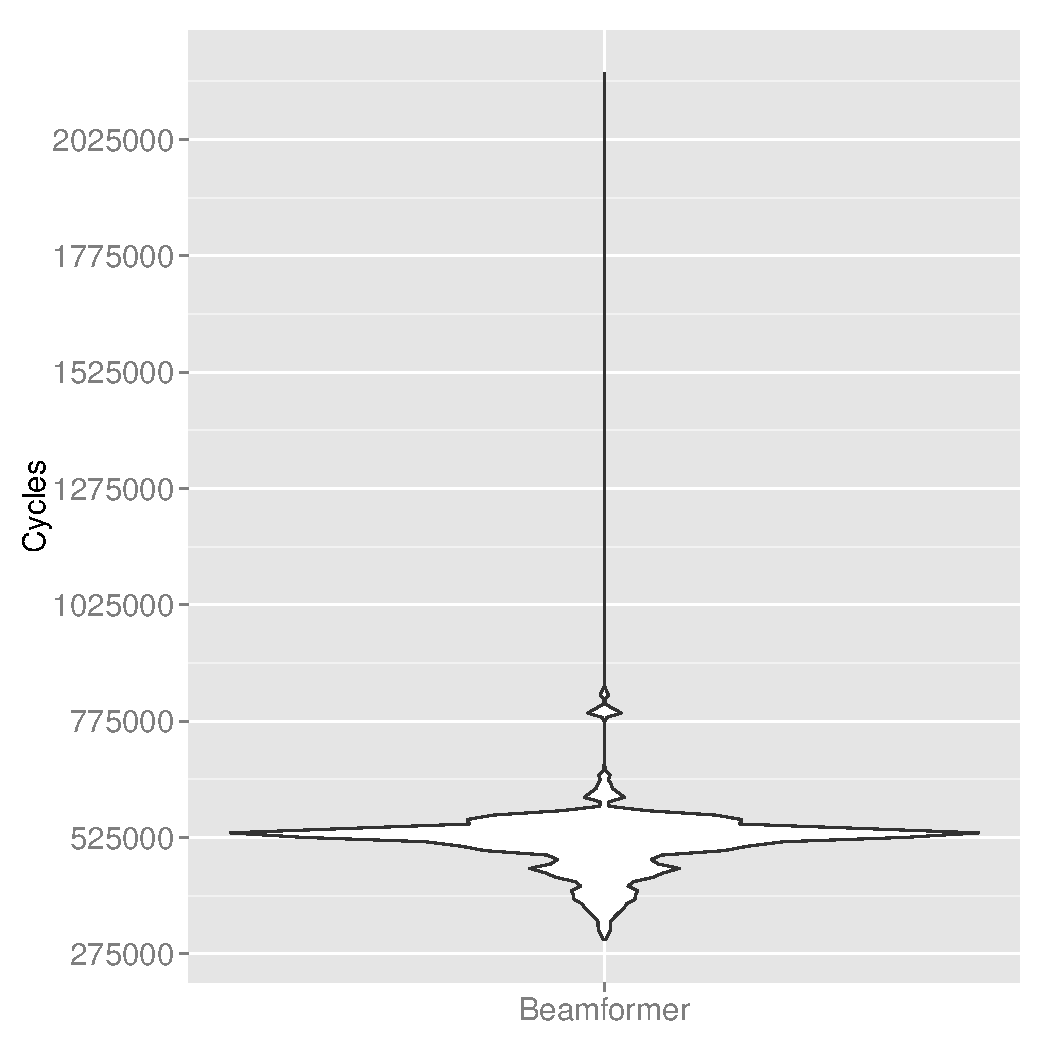
\includegraphics[width=1\textwidth]{streamit-paper/graphics/beamformer_motivation.pdf}
    \caption{Distribution of the runtime for Beamformer resulting from an exhaustively exploration of the hardware/software co-design space.
     The application has been partitioned into different number of threads and core compositions.}
     \label{fig:beamformermotiv}
\end{figure}

This section illustrates the difficulty of finding a good partition and resource allocation.
A simple experiment is conducted where one StreamIt benchmark is taken, \bench{Beamformer}, and partition its tasks into threads and allocate various number of cores to each thread.
A co-design of more than 32,000 combinations (exhaustive space) of thread mappings and core compositions is generated.
Each design point is executed on a dynamic multicore simulator (exact details about the experimental setup are presented later in section~\ref{sec:setup}).

Figure~\ref{fig:beamformermotiv} presents the distribution of the execution times from the co-design space as a violin plot.
For the unfamiliar reader, an intuitive way to think about this violin plot is to consider it as a smoothed histogram rotated by 90 degrees and mirrored.
The majority of the sampled points have a cycle count around 525,000 with the worst points taking more than 2 millions cycles.
The best performance is around 275,000 cycles which is about 2x faster than the majority of the data points.
This shows that finding the right combination of thread mapping and core composition is critical since a wrong choice often leads to suboptimal performance.

This example illustrates the necessity for designing the technique to predict both the optimal number of threads and core composition to use.
The next section will present a more in-depth analysis of the design space before presenting our machine-learning predictive model.



\section{Methodology}\label{chp:stream:sec:setup}
This section describes the setup used throughout this chapter to conduct the design space exploration.
It starts by presenting the overall workflow and then explores briefly some of the features of the benchmarks.
Finally the section explains how the number of design points used throughout the exploration were determined.

\begin{figure}[t]
    \centering
    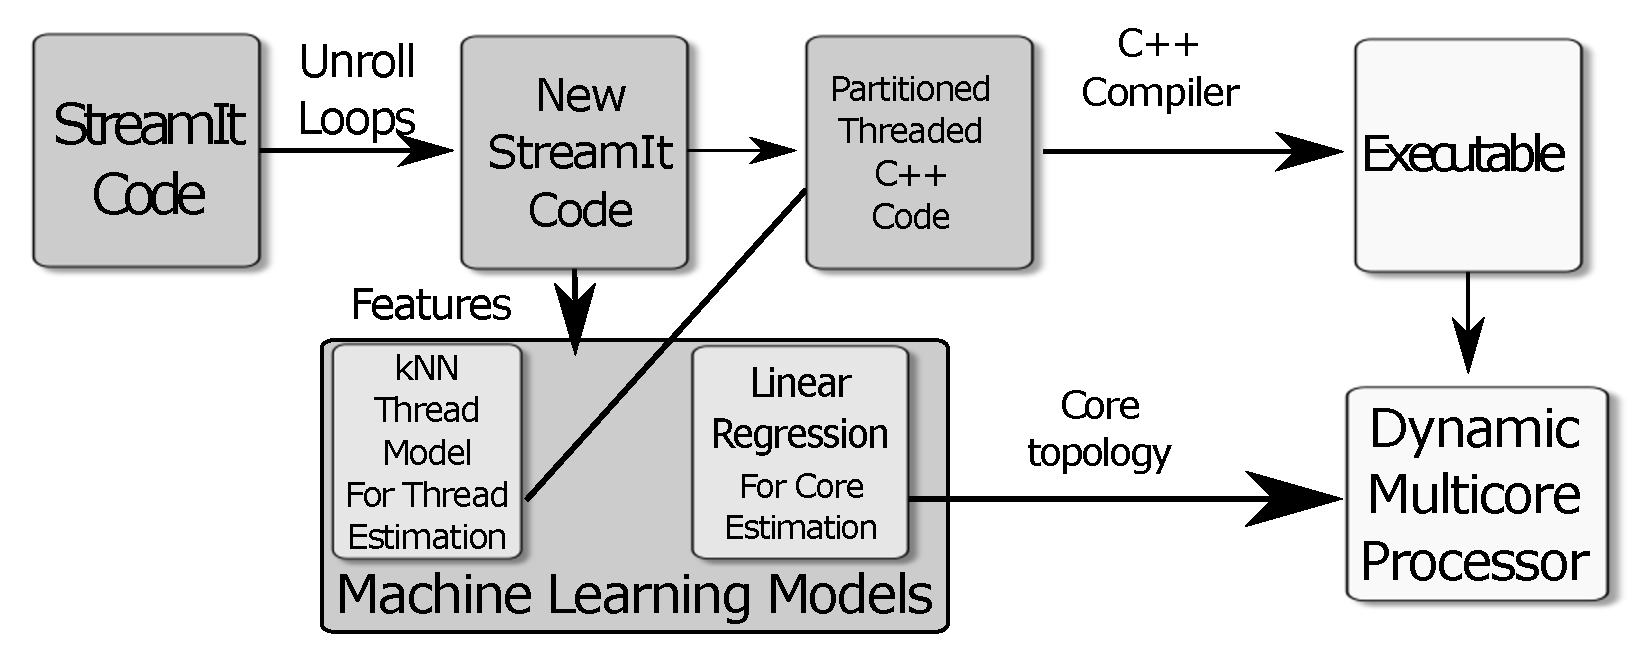
\includegraphics[width=1\textwidth]{streamit-paper/graphics/explanation3.pdf}
    \caption{Description of the workflow.
    Two distinct machine-learning models are used to predict the optimal thread partitioning and core composition based on static code features.}
    \label{fig:overview}
\end{figure}

\subsection{Overview}

\begin{figure}[t]
    \centering
    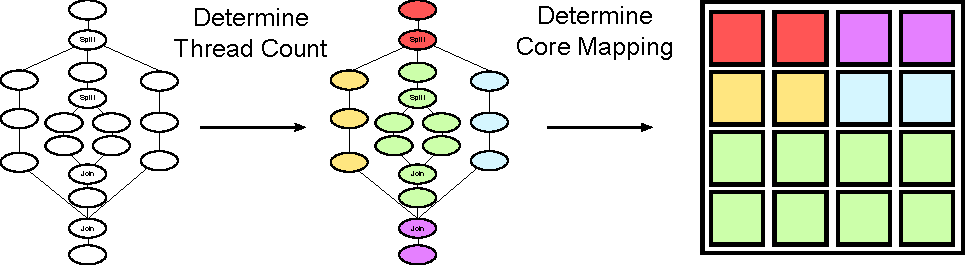
\includegraphics[width=1\textwidth]{streamit-paper/graphics/examplestrem.pdf}
    \caption{Example of a StreamIt program being partitioned into threads (represented by the different colours) followed by assigning cores to each thread.}
    \label{fig:examplestream}
\end{figure}

Figure~\ref{fig:overview} presents the workflow of the system used in this chapter and Figure~\ref{fig:examplestream} illustrates the workflow on a synthetic StreamIt graph.
First, the source-to-source StreamIt compiler is used to unroll loops as this is often beneficial when cores are composed as will be seen later in Section~\ref{sec:streamit:dse}.
Then, static code features such as the program's graph structure are extracted from the StreamIt code through the StreamIt source-to-source compiler.
These features are used as an input to the first machine-learning model that determines how many threads will be required based on an estimate of Thread Level Parallelism (TLP) found in the program.
This information is used to partition the program into threads which is done by the StreamIt compiler which produces a C++ program using pthreads.
This is exemplified in Figure~\ref{fig:examplestream}, the colours filling in the nodes represent the threads each node has been assign to.
This C++ program is then compiled using the compiler for EDGE described in Chapter~\ref{chp:setup} Section~\ref{chp:setup:comp}.

Then, a second machine-learning model is deployed which also analyses static code features extracted from the SteamIt code, once again provided by the source-to-source compiler.
This model decides on the number of cores each thread will have.
This is achieved by estimating the amount of Instruction Level Parallelism (ILP) that can be possibly extracted in each thread and by determining how many physical cores should be fused for that thread.
Finally, the processor is reconfigured to compose the requested resources ahead of time and execute the partitioned program.
For example in Figure~\ref{fig:examplestream}, once the graph is coloured, the machine learning model estimates the potential ILP in each group and assigns a number of cores each thread will execute on.

\subsection{Design Space}

The benchmarks used throughout this chapter are shown in Chapter~\ref{chp:setup} Section~\ref{chp:setup:streamit}.
These applications represent a variety of embedded applications and kernels, from digital signal processing to a matrix-multiplication kernel or band pass filters.
Table~\ref{tab:instancefilt} shows the number of filter instances and SplitJoins for each of the benchmarks.
As a refresher from Chapter~\ref{chp:Background} Section~\ref{chp:bckg:streamit}, SplitJoin filters are functions which distribute and collect data from parallel filters.
The applications feature a different number of SplitJoins which determine the task-level parallelism.
This is to include a variety of situations to test the flexibility of the dynamic multicore processor.
Whilst SplitJoins often facilitate the decision of how to partition the programs into threads, they are not the only way to exploit thread level parallelism.
The applications which do not feature SplitJoins can still be split into threads and will operate in a pipelined fashion~\cite{theis2002streamit}.
For each benchmark the default inputs provided in the repository~\cite{streamitrepo} are used and the default iteration count is set to 10. 

\begin{table}[t]
% The FFT need are variable
  \small
 \begin{tabular} { | l | l | l | l | l | l | }
 \hline
 \cellcolor[gray]{0.7}Type  & \cellcolor[gray]{0.7}Audiobeam&  \cellcolor[gray]{0.7} Beamformer& \cellcolor[gray]{0.7}Bitonic-Sort  &  \cellcolor[gray]{0.7} BubbleSort &  \cellcolor[gray]{0.7}  CFAR\\ \hline
  Filter Instances & 18 & 56 & 82 & 18 & 3 \\ \hline
	\# of SplitJoins &	1 & 2 & 44 & 0 & 0 \\ \hline

 \cellcolor[gray]{0.7}Type  & \cellcolor[gray]{0.7}ChannelVocoder &  \cellcolor[gray]{0.7} FFT&  \cellcolor[gray]{0.7}FFT3 &  \cellcolor[gray]{0.7} FFT6&  \cellcolor[gray]{0.7}FilterBank \\ \hline
  Filter Instances & 53 & 20 & 185 & 99 & 67 \\ \hline 
   \# of SplitJoins &	 1 & 12 & 44 & 96 & 9 \\ \hline 

   \cellcolor[gray]{0.7}Type& \cellcolor[gray]{0.7}FIR &  \cellcolor[gray]{0.7} FMRadio &  \cellcolor[gray]{0.7} InsertionSort &  \cellcolor[gray]{0.7} Matmul-Block &  \cellcolor[gray]{0.7} RadixSort\\ \hline
  Filter Instances& 131 & 29 & 6 & 4 & 13 \\ \hline
  \# of SplitJoins&    0 & 7 & 0 & 7 & 0 \\ \hline

 \end{tabular}
  \caption{Number of filter instances and SplitJoin filters present in each benchmark.}\label{tab:instancefilt}
\end{table}

%\begin{table}[t]
% The FFT need are variable
 % \small
 %\begin{tabular} { | l | l | l | l | l | }
 %\hline
 %  \cellcolor[gray]{0.7}Audiobeam&  \cellcolor[gray]{0.7} Beamformer& \cellcolor[gray]{0.7}Bitonic-Sort  &  \cellcolor[gray]{0.7} BubbleSort &  \cellcolor[gray]{0.7}  CFAR\\ \hline
 % 1 & 2 & 44 & 0 & 0 \\ \hline
 %  \cellcolor[gray]{0.7}ChannelVocoder &  \cellcolor[gray]{0.7} FFT&  \cellcolor[gray]{0.7}FFT3 &  \cellcolor[gray]{0.7} FFT6&  \cellcolor[gray]{0.7}FilterBank \\ \hline
 % 1 & 12 & 44 & 96 & 9 \\ \hline 
 %  \cellcolor[gray]{0.7}FIR &  \cellcolor[gray]{0.7} FMRadio &  \cellcolor[gray]{0.7} InsertionSort &  \cellcolor[gray]{0.7} Matmul-Block &  \cellcolor[gray]{0.7} RadixSort\\ \hline
 % 0 & 7 & 0 & 7 & 0 \\ \hline
% \end{tabular}
%  \caption{Number of split joins present in each benchmark.}\label{tab:splitjoin}
%\end{table}

\begin{table}[t]
\centering
\begin{tabular} { p{5.2cm}  p{1.8cm} }
      \toprule
      \textbf{Parameter} & \textbf{Values} \\ \midrule
      \# of cores in the processor & 16 \\
      \# threads per application & 1 -- 15 \\
      \# cores per thread & 1 -- 15 \\ \midrule
      \# sampled core compositions & 100 \\ 
      \# our sampled space & 1316 \\
      \# total sample space & 32767 \\ \bottomrule
    \end{tabular}
  \caption{Design space considered per application.}
  \label{tab:space}
\end{table}

The parameters and size of the space are given in Table~\ref{tab:space}.
In this study the 16 core DMP defined in Chapter~\ref{chp:setup} Section~\ref{chp:setup:conf} is used.
Having 16 cores allows for a larger variety of configurations, this also represents a processor similar to a tiled embedded system such as Tilera or Raw.
All cores in the DMP are utilised; Core 0 is assigned to the main thread and for runtime management.
This leaves 15 cores available for each application.
Each core is restricted to running only a single thread, as no context switching is supported, which leads to a possible number of threads between 1 and 15.
The core-composition is not used on the master core, leaving 15 physical cores to be distributed to each of the worker threads.
Cores can be composed together to form a composition with up to 15 physical cores, making the total number of cores assigned to a thread between 1 and 15.
Of course, not all cores have to be assigned to a thread, in this case all remaining cores that aren't in a composition or a thread are turned off.
Overall, this leads to a total space size of 32,767 unique combination per benchmark as previously described in Section~\ref{sec:motivation}.

\subsection{Sample Space}

Given a partition, any benchmark that can be split into 15 threads requires 32,767 executions to cover the entire space.
Running the exhaustive exploration of the space for a benchmark requires approximately a week of simulation on a 572+ node supercomputer.
For this reason, a sample of 1,316 random points from the entire space is utilised.
This roughly corresponds to 100 core compositions for each number of threads; the actual number, 1,316 is smaller than 1,500 since for low and high thread counts there are less than 100 possible different core composition.
For example, a single thread can have only up to 15 different core-compositions (1 through 15) whilst 15 threads can only have a single core given to each thread.
\bench{InsertionSort} is the only exception since it can at most only be split into 5 threads leading to 415 sample points.
Overall, the space exploration required one week of simulation on the supercomputer~\cite{ecdf}.

\begin{figure}[t]
  \centering
    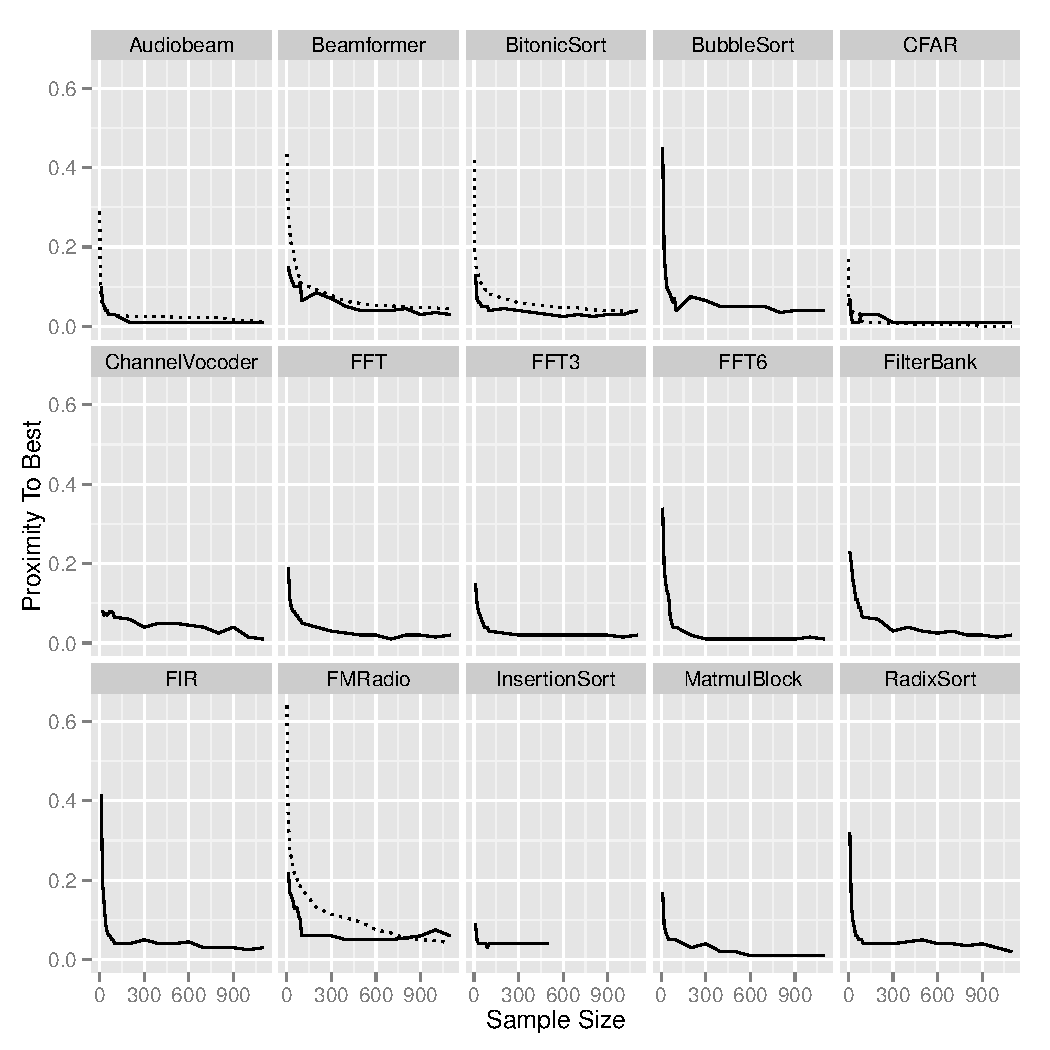
\includegraphics[width=1\textwidth]{streamit-paper/graphics/ESCProx.pdf}
    \caption{Statistical (plain line) and actual proximity (dotted line, this is only done for 5 benchmarks) to best performance using a subset of the sample space.}\label{fig:prox}
\end{figure}

%Define stopping criterion?
To gain confidence that the best configuration from the sample space is indeed close to the real best in the entire space, a statistical model based on the Early Stopping Criterion defined in~\cite{vuduc2003AutomaticPerf} is deployed.
This statistical model estimates, given a sample of the total space, if the best observed performance of that sample space is within a percentage of the statistical best performance, a more detailed explanation can be found in Chapter~\ref{chp:Background} Section~\ref{sec:esc}.
The results demonstrate that the sample space selected is representative of the whole space.

Figure~\ref{fig:prox} shows, for each of the benchmarks, the proximity to the statistical best when increasing the sub-sample space given a maximal uncertainty of 5\%  (\ie minimum 95\% confidence).
As can be seen by the plain line, the model shows that the best sample point is actually within 5\% (0.05 proximity) of the best for all the benchmark.
The proximity is measured by taking the best currently observed point and comparing it to the latest discovered point.
To further prove that the statistical model based on the Stopping Criterion is indeed accurate, an exhaustive exploration of five benchmarks is conducted.
The dotted line in figure~\ref{fig:prox} shows the actual proximity to the best for \bench{Audiobeam}, \bench{Beamformer}, \bench{BitonicSort}, \bench{CFAR} and \bench{FMRadio}.
As can be seen after 1316 samples, the achieved performance is actually very similar to the one predicted by the statistical model, hence confirming prior work~\cite{vuduc2003AutomaticPerf}.
To summarise, it can be concluded that the best point found in the sample space of 1,316 points is at least within 5\% of the real best in the exhaustive space with 95\% confidence.

\subsection{Synthetic Benchmarks}

\begin{table}[t]
% The FFT need are variable
  \small
 \begin{tabular} { | l | l | l | }
 \hline
 & Av. Number of SplitJoins & Average Number of Filter Instances \\ \hline
 Selected Benchmarks & 14 & 52 \\ \hline 
 Synthetic & 22 & 64 \\ \hline
 \end{tabular}
 \caption{Data on the synthetic benchmarks compared to the selected benchmarks}~\label{tab:synthvsreal}
 \end{table}

One of the difficulties of building a machine learning based model for StreamIt is the lack of a large amount benchmarks available~\cite{wang2013partitionstreamit}.
To overcome this problem generating synthetic benchmarks can be a solution~\cite{cumminsopencl2017}.
Thus synthetic StreamIt benchmarks are generated and statistics are gathered from them in a similar style as in~\cite{wang2013partitionstreamit}.
In this chapter, the synthetic benchmarks are used to build a model for predicting the number of threads, which will be described later in section~\ref{sec:ml}

%Cite repository
To ensure that the synthetic benchmarks are representative of realistic benchmarks they are created using filters from a set of example StreamIt programs found in the example directory in the repository.
30 different possible filters with different incoming and outgoing rates and different inputs and outputs types are used to increase the variety of the dataset.
To ensure that the synthetic benchmarks are similar to real benchmarks, the total number of filters and split joins are within the average of the realistic benchmarks.
Table~\ref{tab:synthvsreal} gives the average number of SplitJoins and filter instances for the synthetic benchmarks vs the real benchmarks used in this chapter.
As can be seen, the synthetic benchmarks, on average, have more SplitJoins than the real benchmarks; this is due to the fact that a few of the benchmarks presented in the chapter don't have SplitJoins at all which can quickly reduce the average.
%Maybe say a bit more here.
Since these benchmarks are built to be used for predicting the number of threads an application should use, and SplitJoins are explicit declarations of task-level parallelism, having a higher average number of SplitJoins is not detrimental to building the model.


\section{Design Space Exploration}\label{sec:streamit:dse}
This section describes the exploration of the software/hardware co-design space.
The software side includes partitioning the program, determining the number of threads and the specific source-level optimisations.
The hardware side is about finding out the best core composition that maximizes performance for a given partitioning.

\subsection{Thread Partitioning}

This section first starts with analyzing the impact of thread partitioning on performance.
In this section, the term optimal number of threads defines the number of threads which results in the best performance for any given benchmark.
Thread partitioning is about deciding how many threads to create and how to partition StreamIt filters into these threads.

To simplify this study, the default streaming partitioner is used to decide on how to allocate filters to threads which is based on simulated annealing~\cite{simulatedAnnealing1983}.
On the hardware side, two scenarios are considered: the ``without composition scenario'' where there is exactly one core per thread and the ``with composition scenario'' where each thread receives between 1 and 15 cores.
Figure~\ref{fig:threadtrend} shows how performance varies under both scenarios as a function of the number of threads.
In this figure, the ``with composition scenario`` uses points from the sample space that result in the fastest execution time for a given number of threads.
Regardless of how cores are composed it can be observed that curves for a benchmark follow the same trend.
As can be seen in Figure~\ref{fig:threadtrend}, the optimal number of threads using core composition is very similar to the scenario without composition as both curves follow the same performance trends.
This is due to the fact that StreamIt is oriented towards task-level parallelism and thus, multithreading will be a natural fit for performance improvements whilst core-composition may have less of an effect overall.
As Figure~\ref{fig:threadtrend} shows that the performance trends for both with and without composition are similar when it comes to thread counts, this  means that the optimal number of threads for a benchmark can be estimated independently from the hardware composition.
The system can therefore proceed in two stages: first determine the optimal number of threads and then decide on a core composition.

Figure~\ref{fig:threadtrend} also shows that the performance of most benchmarks starts to deteriorate passed a certain number of threads making it critical to not over-allocate threads.
This number of threads varies between benchmarks, thus it motivates the use of machine learning to decide the optimal number of threads to use.
Finally it is important to observe that executions without compositions always perform worse.
This demonstrates that composing cores is essential to obtain the best performance from a workload.


\subsection{Core Composition}

\begin{figure}[t]
  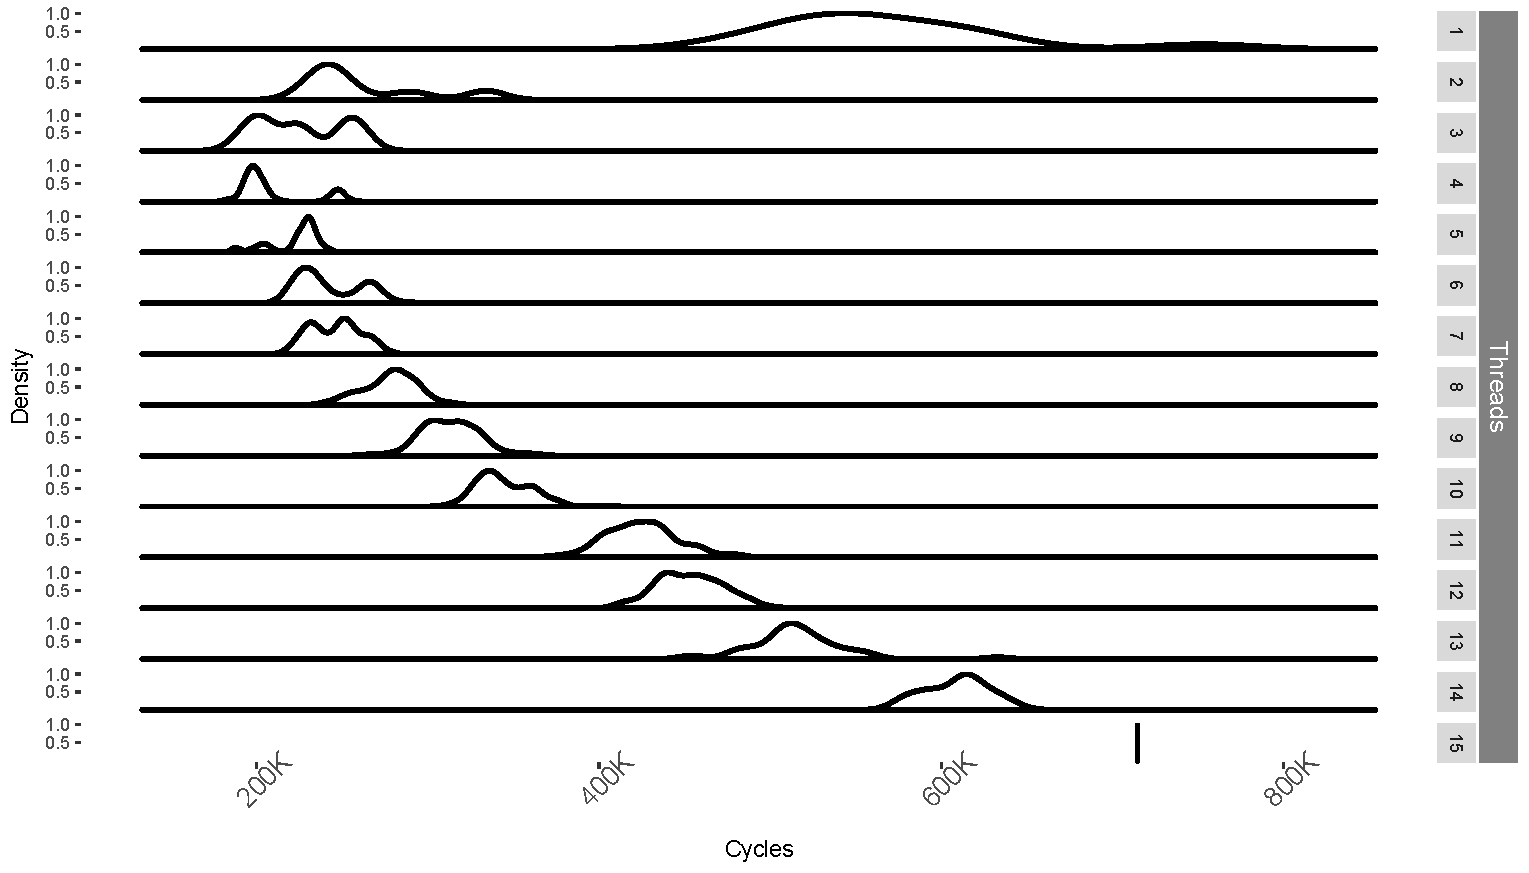
\includegraphics[width=1\textwidth]{streamit-paper/graphics/filterbank_tot.pdf}
  \caption{Distribution of FilterBank performance when modifying the amount of threads and compositions.}\label{fig:fbtotal}
\end{figure}

Using core composition, the processor fuses a number of cores and associates them to a thread to increase the thread's performance.
Whilst this flexibility is advantageous, choosing the right amount of cores for a given thread is difficult due to the large number of possible configurations~\cite{gulati2008multitaskingdmc}.

Figure~\ref{fig:fbtotal} shows how threading and core-compositions affect performance for the \bench{FilterBank} benchmark.
The curves represent the density distribution for different core compositions as a function of the number of threads.
The right hand side Y-axis represents the number of threads present in the current version of the benchmark whilst the left Y-Axis represents the density normalized by the total number of points in the design space.
For each of the threaded versions the benchmark runs using 100 different core-compositions.
The density curve for thread 15 is a single point as there exists only a single composition, so a line is drawn to represent where that point lies.

The width of each of the curves represents the influence of composition on the \bench{FilterBank}'s performance for a given number of threads.
For this benchmark, the impact of having core-composition enabled often leads to a 1.5x speedup compared to running only in multi-threaded mode; this can be seen for 1 to 4 threads.
Interestingly, as more threads are used, performance worsens, echoing the results shown in the previous section.
This is due to the fact that when the number of threads is increased, synchonization between threads will increase whilst the potential number of corse which can be fused decreases.
In the case where the application does not feature highly parallel tasks, de-prioritising core compositions can negatively impact performance.
This signifies that for the benchmark \bench{FilterBank}, it is more important to fuse cores with a small amount of threads rather than add more and more threads to the application.


\begin{figure}[t]
  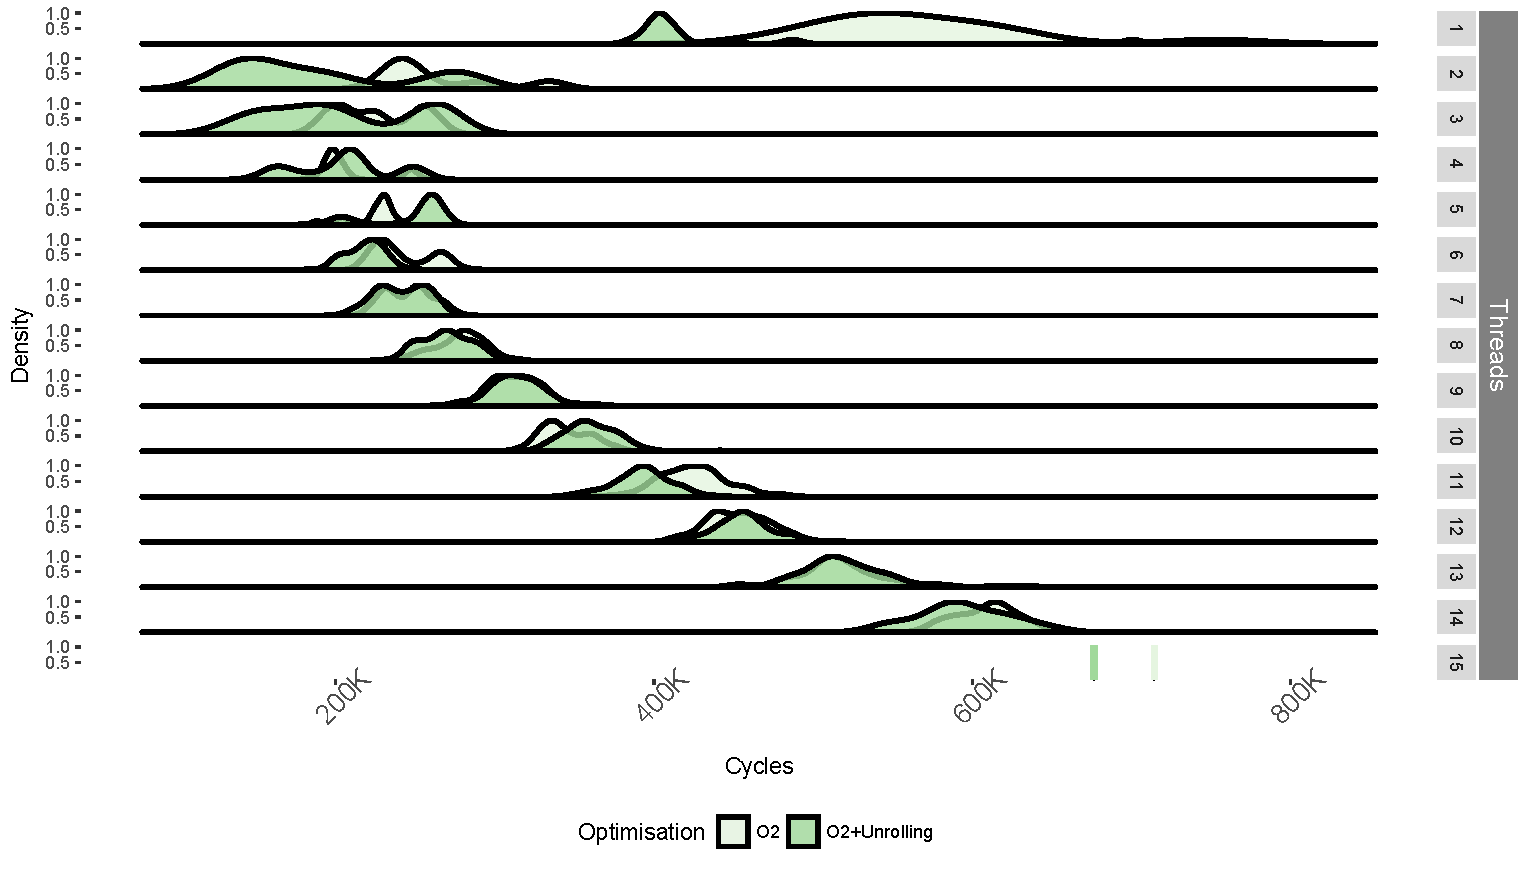
\includegraphics[width=1\textwidth]{streamit-paper/graphics/filterbank_unroll.pdf}
  \caption{Distribution of FilterBank performance when modifying the amount of threads, composition and unrolling factor.}\label{fig:fbunroll}
\end{figure}


\subsection{Impact of Loop Transformation}
As seen in Chapter~\ref{chp:Background}, composing cores exploits block-level parallelism by running multiple EDGE blocks on a logical core.
As physical cores in a logical core must communicate to submit block address predictions, and commit information to each other, having a small number of blocks will reduce the communication overhead.
In a core-composition, commit information can be a core informing another core that it has become the non-speculative core, or that registers can be read or written to.
Since physical cores can fetch more than a single block when the blocks are made of a small number of instructions, if the program being executed is comprised of small blocks this will cause a composition to fetch a high amount of blocks.
Thus finding methods to increase the average size of the blocks can lead to reduced overhead.
One method of increasing the size of the blocks is through loop unrolling.
This section therefore analyses the impact of loop unrolling on the StreamIt benchmarks.

In this Chapter, unrolling is done at the source level via a flag passed to the StreamIt source-to-source compiler.
Given a number of times the loops must be unrolled, the StreamIt source-to-source compiler will generate the multi-threaded C++ code with the loops unrolled.
Figure~\ref{fig:fbunroll} presents an example of how loop unrolling affects performance on the \bench{FilterBank} benchmark.
The graph presents the same information as Figure~\ref{fig:fbtotal} but comparing .
Figure~\ref{fig:fbunroll} shows that unrolling loops for \bench{FilterBank} can improve performance by up to 1.42x compared to the fastest non-unrolled version.
Another observation is that the best execution times for each of the threaded versions when unrolling does not follow the same trend seen in Figure~\ref{fig:threadtrend}.
The leftmost curve performance peaks at two threads whereas the rightmost peaks at 3 compared to 4 in the non-unrolled version.

\begin{figure}[t]
  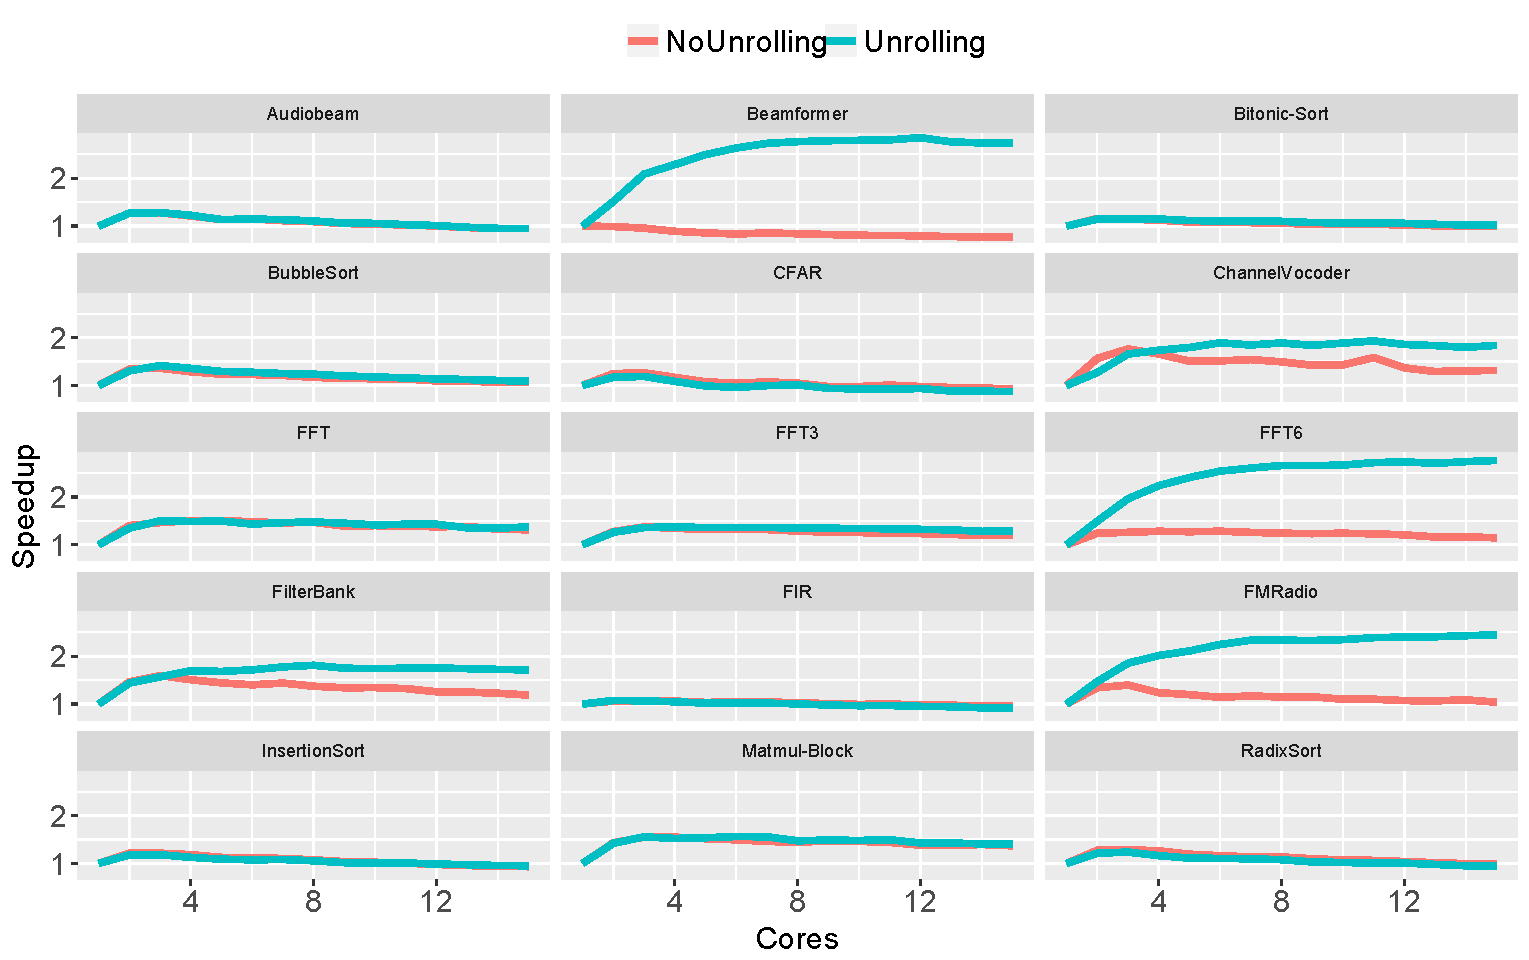
\includegraphics[width=1\textwidth]{streamit-paper/graphics/unrolling_vs_no_single_core.pdf}
  \caption{How unrolling affects how much performance can be obtained via core-composition on the single-threaded versions of each benchmarks.}\label{fig:unroll_summary}
\end{figure}

Figure~\ref{fig:unroll_summary} goes into more details on how unrolling affects the amount of speedup obtained by running each of the StreamIt benchmarks on a single thread using different number of cores in the composition.
In this figure, the X axis represents the number of cores in the composition, ranging from single core to 15.
The Y axis compares the execution time in number of cycles for the benchmark using a single core vs a given core-composition.
The colours of the lines represent with and without unrolling.
As can be seen, for the set of benchmarks used throughout this chapter, five benchmarks benefit from unrolling.
These benchmarks are \bench{Beamformer}, \bench{ChannelVocoder}, \bench{FFT6}, \bench{FilterBank} and \bench{FMRadio}. 

\begin{figure}[t]
  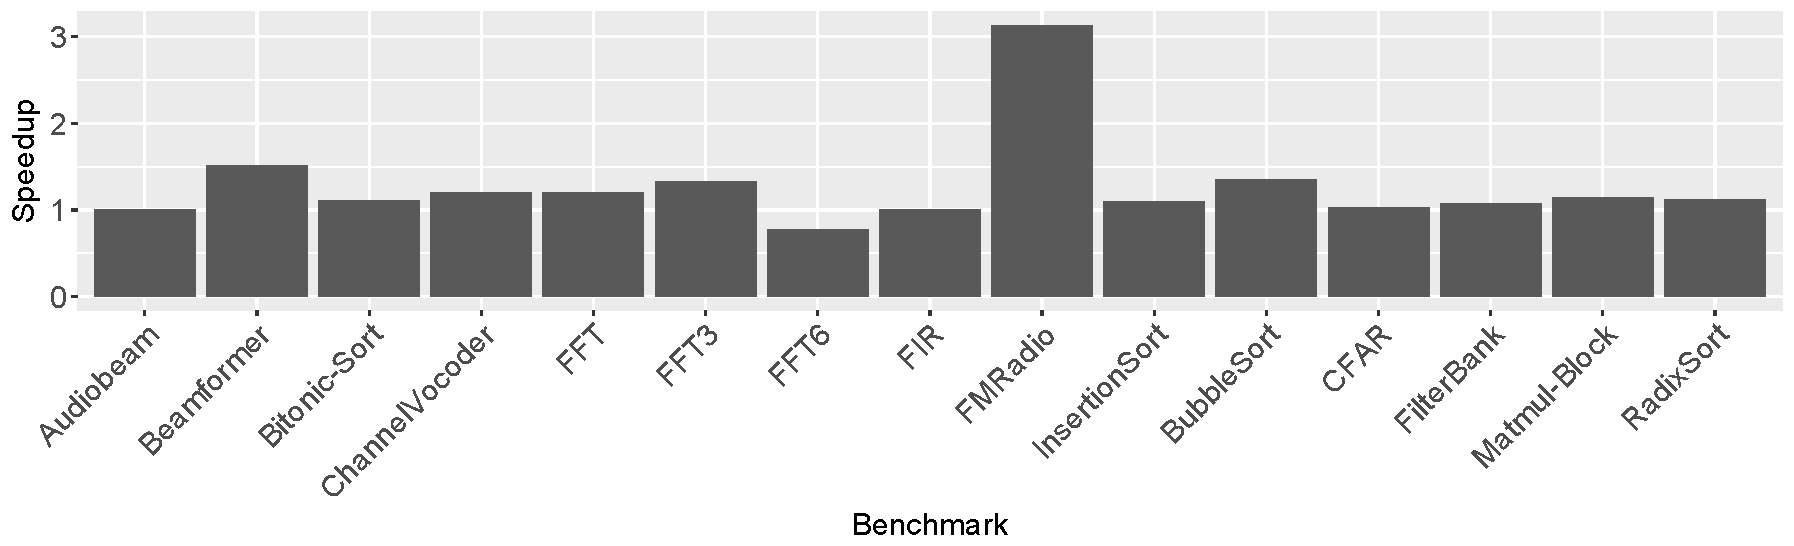
\includegraphics[width=1\textwidth]{streamit-paper/graphics/unroll_speed_bars.pdf}
  \caption{Speedup obtained .}\label{fig:unroll_bars}
\end{figure}
Figure~\ref{fig:unroll_bars} complements Figure~\ref{fig:unroll_summary} by showing the speedup obtained by unrolling loops when executing the benchmark on a single core.
On average, the information shown in Figure~\ref{fig:unroll_bars} coincides with the data shown in Figure~\ref{fig:unroll_summary}: benchmarks that don't scale also see no difference in performance when loop unrolling is called.
For the benchmarks that do not scale with unrolling; this is most certainly due to the for loops containing conditional statements which may keep the blocks size small.
When a loop that holds multiple conditional statements is unrolled, conditional statements may not be fused into a single block; thus the block size does not change.
Benchmark \bench{FMRadio} sees a 3x improvement compared to the non-unrolled version, this is due to the fact that all the loops are fully unrolled, reducing the total number of instructions required to execute the task.
For the \bench{FFT6} benchmark, unrolling loops will actually cause the single-core version to be slower than its not unrolled version.
%I think this is due to a refreshing performance thing
This is due to the fact that for \bench{FFT6}, the source to source unrolling adds intermediate variables in the loop which increase the number of loads and stores.
Whilst it may be slower on a single core, as seen in Figure~\ref{fig:unroll_bars}, having a core-composition running the thread will still result in faster execution that without loop-unrolling.

Figure~\ref{fig:unroll_size} shows the influence of loop unrolling on the average size of an EDGE block for each of the benchmarks.
The size represents the number of instructions exected in each of the EDGE blocks.
As can be seen, the data for \bench{Beamformer} and \bench{FFT6} in Figure~\ref{fig:unroll_size} corroborate with the idea that larger block sizes will result in better performance when fusing cores.
However whilst benchmarks \bench{ChannelVocoder}, \bench{FilterBank} and \bench{FMRadio} also see an increase in blocksize, it is not as important and averages out at a 1.22x increase.
%Be clearer here.
That said, even a small amount of increase can help improve the scalability of core-composition.

\begin{figure}[t]
  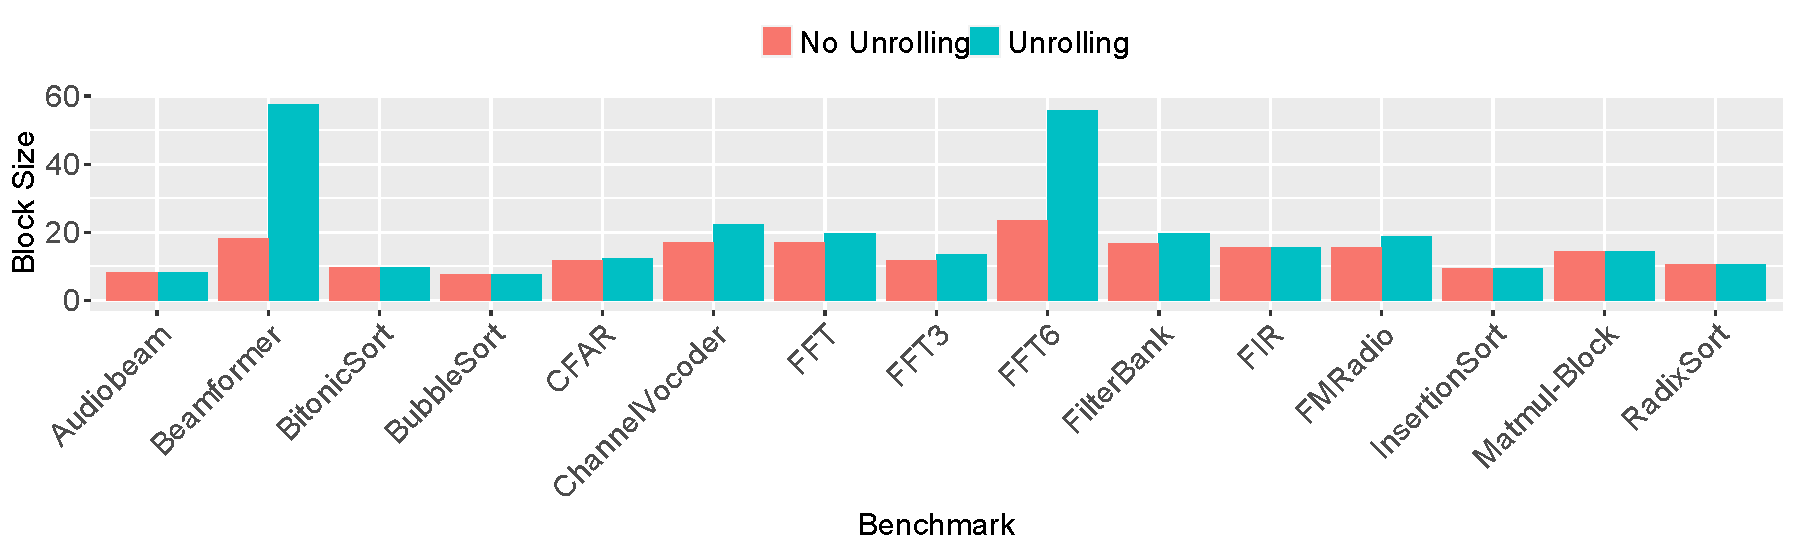
\includegraphics[width=1\textwidth]{streamit-paper/graphics/unrolling_size.pdf}
  \caption{Average size (in instructions) of blocks executed with and without unrolling for each benchmark .}\label{fig:unroll_size}
\end{figure}

Overall, this section has shown that loop unrolling can improve performance by increasing the size of blocks for the benchmarks which helps improve the efficiency of core-compositions.

\subsection{Co-Design Space Best Results}


This section  presents the results of the entire co-design space exploration.
Figure~\ref{fig:overviewhist} characterizes how much of a performance increase, over a baseline of a single-core single-thread with O2 optimisations, can be obtained with and without unrolling.
For each benchmark, the \textit{THREAD} bar represents the maximal speedup obtained by dividing the program into threads without fusing cores.
The \textit{CORE} bar represents the best speedup when the benchmark is executed in a single thread and fuse cores.
\textit{BOTH} represents the best speedup obtained for each benchmark using a combination of \textit{THREAD} and \textit{CORE}.
Finally, for each benchmark, the results are obtained for both an unrolled and not unrolled version to compare how the compiler optimisation affects performance.
Figure~\ref{fig:overviewhist} shows that when loops are not unrolled, composing cores will not greatly improve performance.
This is due to the fact that the amount of ILP found in filters without the unrolling is too little for there to be any benefit of composing cores.

In the scenario where there are no specific optimisations for composition, multithreading will be the main source of performance.
This can be seen when studying the geometric mean,without unrolling.
Finding the optimal number of threads gives a speedup of 1.92 compared to 1.33 when using only core composition, which is an improvement of 44\%.
This changes when taking unrolling into account as the core compositions can be used more efficiently.
In this case, the speedup obtained from only composing cores is only 13\% worse than using only threads.
For the \bench{FMRadio} benchmark, unrolling makes using only core-composition better than only using threads.
This information corroberates with the data seen in Figure~\ref{fig:unroll_summary}; it presents a unique case where the effect of core composition is important enough to change the dominant performance enhancer.
The performance increase obtained via the source-level loop unrolling via the compiler demonstrates that some modifications to the code must be done to ensure optimal use of the dynamic multicore processor.
%Thus loop unrolling demonstrates that the StreamIt programs must be modified to take advantage of the core composition.

Overall the results demonstrate that multi-threading is the prevalent leader of performance, even with unrolling turned on.
This is natural as StreamIt applications are naturally geared towards TLP as most programs have at least one SplitJoin as seen in the Table~\ref{tab:splitjoin} which gives the number of split-joins per benchmark.
Benchmarks with SplitJoins will naturally benefit from splitting the program into threads~\cite{thiesStreamit2010}.
%Make sure this is 100% true but as far as I remember this is the case
Those that do not feature SplitJoins can still be parallelised by splitting a Pipeline into multiple parts.
For example, benchmark \bench{FIR} features no SplitJoins, yet splitting the Pipeline in 2 will result in a 1.40x speedup.
However, it is important to note that whilst finding the optimal thread mapping may result in higher performance improvements than finding the optimal composition for a single thread, the best performance is always obtained through a combination of both optimizations.
For cases such as \bench{BeamFormer} the optimal pairing results in a 1.8x speedup compared to simply finding the best multit-threaded version.
On average, the optimal combination leads to a 1.5x performance increase compared to only multithreading.

\begin{landscape}
\begin{figure}\hspace{-1em}
    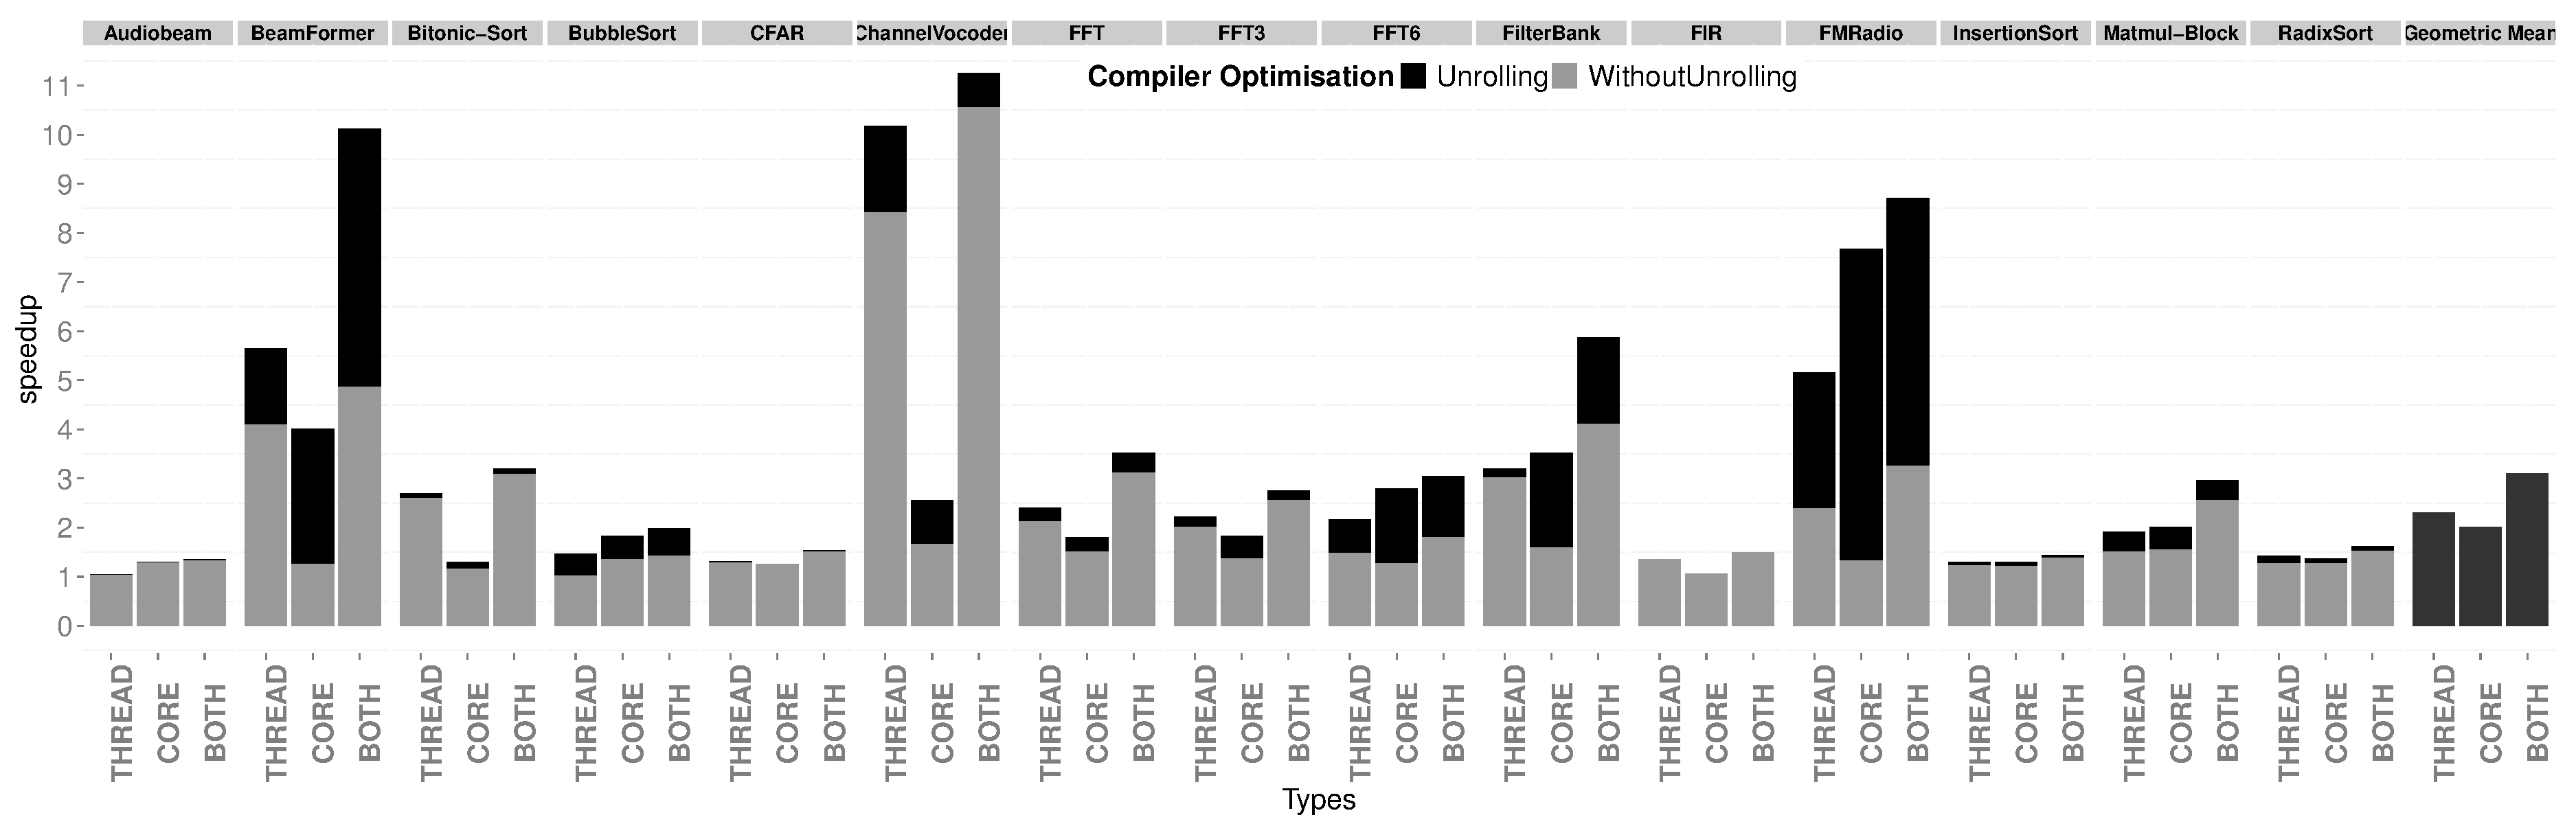
\includegraphics[width=1\linewidth,keepaspectratio]{streamit-paper/graphics/threadcompbench.pdf}
    \caption{Speedup obtained by choosing best core composition, best
      thread number and the combination of both optimisations. The baseline for the speedup measurement is single core, single thread execution using O2 compiler optimisations. Higher
      is better.}\label{fig:overviewhist}
\end{figure}
\end{landscape}
\subsection{Summary}
This section demonstrated that each parameter has a large effect on the performance of the workload.
Regardless of using core composition or not, there exists for each benchmark an optimal number of threads.
Unrolling is effective at exposing more opportunities for composition due to increased block sizes but there is a balance to strike between extracting large blocks and TLP.
Figure~\ref{fig:overviewhist} shows there is a 3x benefit (overall) by automating the partitioning of both the software (threads) and hardware (cores).



%\section{Machine Learning Models}
\section{Creating the model for thread and core configurations}\label{sec:ml}
%\section{Predicting the Best Number of Threads}
% Small intro, re-explain that finding thread/core pairing is complicated and thus ML is a good idea.
As seen in the previous section, selecting the right number of threads and a good combination of cores is difficult.
This difficulty arises from trying to balance between exploiting larger composed cores with block speculation and ILP and between exploiting a larger number of logical cores via TLP.

The problem can be decomposed into two stages; first, determining the right number of threads and then selecting a good core composition.
In this section, two machine-learning models that predict the best thread partitioning and core composition to maximize performance are presented.

\subsection{Synthetic Benchmark Generation}

One of the difficulties of building a machine learning based model for StreamIt is the lack of benchmarks available~\cite{wang2013partitionstreamit}.
Whilst there exists at least 30 realistic applications for StreamIt~\cite{theis2010empericalcharstreamit} this is simply not enough to create a large enough data set.
To overcome this problem generating synthetic benchmarks can be a solution~\cite{cumminsopencl2017}.
Thus synthetic StreamIt benchmarks are generated and statistics are gathered from them in a similar style as in~\cite{wang2013partitionstreamit}.
To ensure that the synthetic benchmarks are representative of realistic benchmarks they are created using filters from a set of micro-kernels found in some StreamIt applications.
30 different possible filters with different incoming and outgoing rates and different inputs and outputs types are used to increase the variety of the dataset.
To ensure that the synthetic benchmarks were similar to real benchmarks, the total number of filters and split joins are within the average of the realistic benchmarks.

For each generated application, 15 different threaded versions are generated.
Each of these versions is ran using a single core per thread and the cycle count is recorded.
This was repeated for 1000 unique randomly generated applications and record the best number of threads each time.

Once the benchmarks have been generated, the next step consists of gathering features for each applications.
In order to build the two machine learning models an initial set of over 50 features are extracted from StreamIt programs.
These features were extracted using pre-existing analytical tools within StreamIt and some counters added specifically for this chapter.
As 50 features may not necessarily contain any valuable information, the features selected for the models were determine through correlation analysis.
%In this section, when discussing correlation we specifically look at which variables correlate with the optimal number of threads.

\subsection{KNN Model}
In this section, variables which correlate with the optimal number of threads are explored.
These features are used by the model to make a prediction about the number of threads to use.
Figure~\ref{fig:corr} shows the 10 variables that correlate the most with determining the optimal thread number.
In StreamIt the term multiplicity references the number of times a filter will have to execute in a time slice when the graph is in a steady state~\cite{gordon2002streamcomp}.

\begin{figure}
  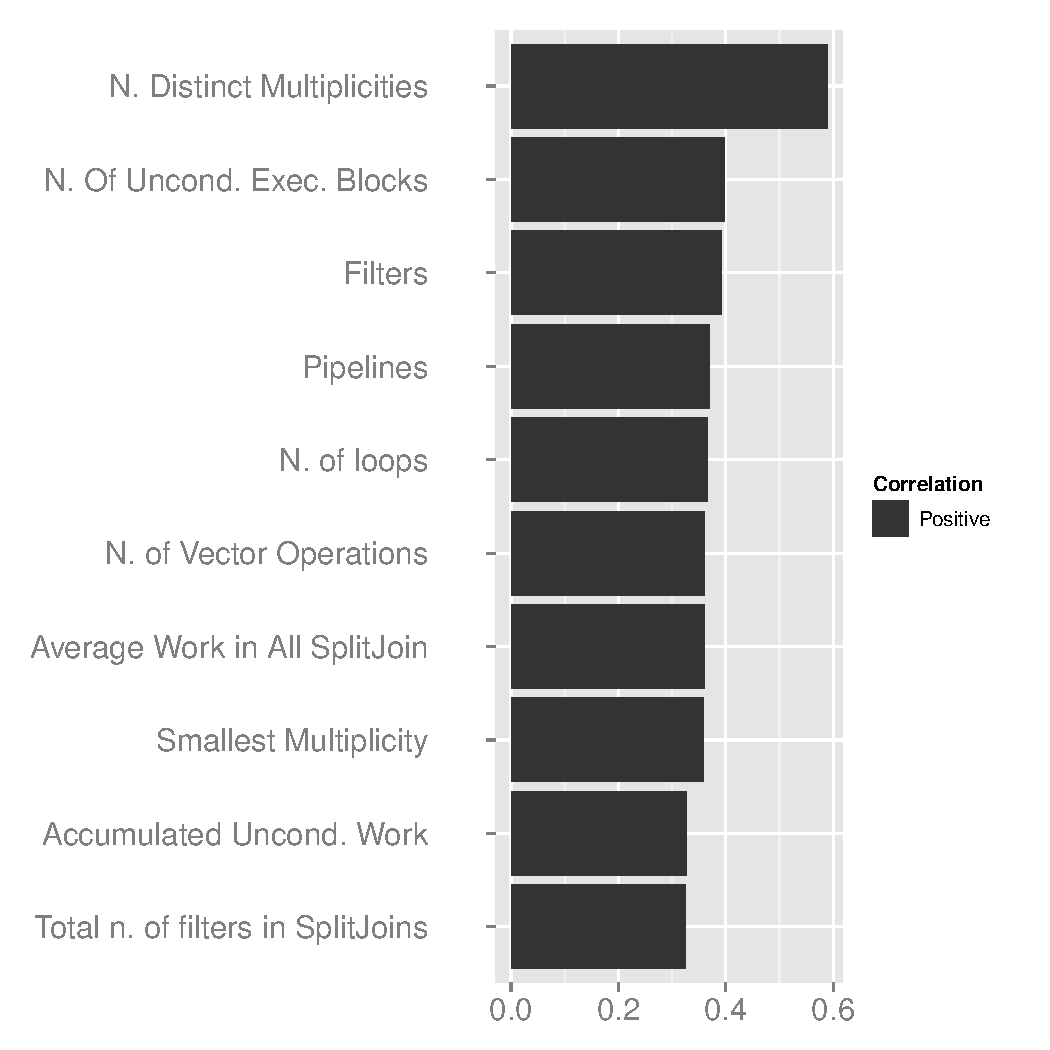
\includegraphics[width=1\textwidth]{streamit-paper/graphics/corrGraph.pdf}
  \caption{The ten highest correlating features with the best number of threads for 1000 synthetic benchmarks.}\label{fig:corr}
\end{figure}
 
\vspace{5em}
The 10 features can be described as followed:
\begin{itemize}
\item Number of Distinct Multiplicities: the variety of different execution rates of filters per time slice.
\item Number of unconditionally executed blocks: amount of operations in a filter that always execute.
\item Filters: number of filters found in the benchmark.
\item Pipelines: number of pipelines found in the benchmark.
\item Number of Loops: amount of loops present in the benchmark.
\item Number of Vector Operations: amount of potential vector operations found in the benchmark.
\item Average Work in all SplitJoins: average amount of operations per SplitJoin.
\item Smallest Multiplicity: The smallest execution rate of a single filter.
\item Accumulated Unconditional Work: Total number of operations in all filters which must be executed.
\item Total Number of filters in SplitJoins: Amount of filters that are found in SplitJoins.
\end{itemize}

According to Figure~\ref{fig:corr} the highest correlating value is Number of Distinct Multiplicitie found in the StreamIt application.
There are very little variables that highly correlate beyond Number of Distinct Multiplicities.
A high number of distinct multiplicities implies that the StreamIt application features an important amount of filters with different execution rates.
This means that certain filters may be local bottlenecks in a Pipeline for example.
When the number of distinct multiplicities is high this requires more threads to group filters with similar multiplicities together.
For example, the benchmark \bench{ChannelVocoder} only has 66\% of its filters sharing the same average multiplicity~\cite{theis2010empericalcharstreamit} of 50, with a minimum multiplicity of 1. 
The benchmark features a single SplitJoin yet when recalling section \ref{sec:streamit:dse}'s Figure~\ref{fig:overviewhist} \bench{ChannelVocoder}'s performance is greatly improved via multi-threading.
The number of threads also depends on certain structural features such as Pipelines, SplitJoins and number of Filters.
Yet, these variables seem to hold less influence on the number of threads a program needs than the different multiplicities found in the graph.
This is most certainly due to the fact that whilst SplitJoins make parallelizable areas more visible, the amount of work contained in each stream of the SplitJoin, especially when this size is small, may actually make parallelizing the program worse due to ratio of communication to computation.
It is also important to understand that a high number of Pipelines implies the use of SplitJoins.
This is due to the fact that a StreamIt application with no SplitJoins will feature only a singe Pipeline, thus a larger number of pipelines implies at least one SplitJoin.\\

A k-Nearest Neighbor (kNN) model is deployed to determine the number of threads to use for an application.
Given a new application, the kNN classifier determines the $k$ closest generated applications.
The distance between the features is measured using the Euclidean for each application.
Once the set of $k$ nearest neighbors is identified, the model simply averages the best number of threads for each of the $k$ nearest neighbors to make a prediction.
The parameter $k$ was determined experimentally using only the generated benchmarks.
A value of $k=7$ was found to lead to the best performance.
The features chosen are the ten variables displayed in Figure~\ref{fig:corr}.

Cross validation is used to determine the efficiency of the model by observing how close a classification is to the measured best thread number.
Using cross validation the model generated in this chapter has a 33\% accuracy of getting the exact best thread number.
The accuracy increases to 57\% when allowing a prediction to be 1 thread away from the best and 67\% when 2 threads away.
On average, having a thread number that is +/- 1 away from the optimal thread count only incurrs a 12\% performance penalty.
For a distance of +/- 2 this increases to 19\%.
This penalty was measured by comparing the performances of the synethtic benchmarks using only multithreading.



%\section{Predicting Core Composition}
\subsection{Predicting the size of a core composition}
In Section~\ref{sec:streamit:dse}, Figure~\ref{fig:threadtrend} showed the performance of each of the 15 benchmarks when partitioning them into threads with and without core-composition.
In both cases, the number of threads is often similar.
The section also demonstrated that loop unrolling can improve the performance of core composition.

Since core composition is used to improve the performance of a single-working-thread, it is important to take into consideration that partitioning the software into threads facilitates the core estimation per thread.
Without determining a number of threads before predicting the number of cores the core-composition model has no information as to the number of threads or the structure of each thread.
In this situation, the core-composition model would either have to make its own estimates as to the thread count, or make a general prediction for a single-working-thread.
Therefore predicting core-composition comes after predicting the number of threads.

\subsubsection{Gathering Training Data for Core-Composition}
For this section the single-working-threaded version of the StreamIt benchmark are used to determine the optimal number of cores in order to explore all possible core composition sizes.
Some of the multi-threaded versions of benchmarks can be used to add extra data-points to build the model, however not all thread-counts are suitable.
One of the difficulties of adding data-points from the highly threaded versions of an applications is that each thread will only be able to have a very small core-composition.
For example, if the 15 threaded version of a benchmarks is added as data points to the model, then each of the feature vectors for this version would have a single core attributed to it.
This is due to the fact that in the 15 threaded versions of benchmarks each thread can only have a single core due to the number of cores on the DMP.
Yet, these threads could potentially benefit from core-composition, so adding them as data points to the model skews future predictions as the feature vector for each thread would associate the features to use only a single core.
Thus high-threaded versions of applications must be ignored to avoid having incorrect suggestions for core-composition sizes.

For the exploration of core composition, the 15 StreamIt benchmarks explored throughout the design space exploration are used. %explain why.
To increase the amount of data available, multiple versions of the benchmarks using different amounts of unrolling are included in the search space.
Four different levels of unrolling are used in to build the model: 0,4,16 and 64.
To determine the optimal number of cores only the training data that has a performance within 1\% of the best is selected.

\begin{figure}[t]
\centering
  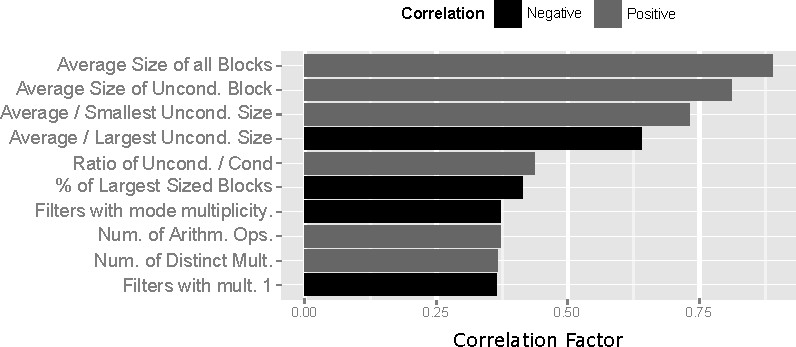
\includegraphics[width=1\textwidth]{streamit-paper/graphics/corrGraph_remix2.pdf}
  \caption{The ten highest correlating features with the optimal number of cores.}\label{fig:corrCore}
\end{figure}


\subsubsection{Correlation Analysis}

Figure~\ref{fig:corrCore} shows the highest correlating features with the optimal number of cores.

The ten features can be described as follows
\begin{itemize}
\item Average Size of All Blocks: Average number of operations per block of code.
\vspace{-1em}
\item Average Size of Unconditional Blocks: Average number of operations per blocks that must execute unconditionally.
\vspace{-1em}
\item Average / Smallest Unconditional Size: The ratio between the average size of a block compared to the smallest size of unconditional blocks.
\vspace{-1em}
\item Average / Largest Unconditional Size: The ratio between the average size of a block compared to the largest size of unconditional blocks.
\vspace{-1em}
\item Ratio of Unconditional Blocks to Conditional Blocks.
\vspace{-1em}
\item Percentage of blocks that have the largest number of operations.
\vspace{-1em}
\item Filters with mode multiplicity: number of filters that have the average mode multiplicity.
\vspace{-1em}
\item Number of arithmetic operations found in the program.
\vspace{-1em}
\item Number of distinct multiplicites found in the program.
\vspace{-1em}
\item Number of filters that have a multiplicity of 1.
\end{itemize}


The features are very different from the ones presented in Figure~\ref{fig:corr} and overall there are features which correlate higher with core-compositions than number of threads.
The highest correlating value, which is the average size of a block, has a correlation factor of 0.88.
It is important to note that the concept of an operation here is at the StreamIt level and not the architectural level.
This is because the machine learning model will get information from the source-level StreamIt translation.
With that in mind, the number of operations will correlate with the number of instructions found at the instruction level.

The second feature is similar to the first but only takes into account blocks that will be executed unconditionally.
Blocks found in loops are excluded for this metric as there is still some form of condition for those blocks to be executed.
The next two features compare the average size of an unconditional block to the largest and smallest unconditional block.
The fifth feature measures the ratio of the number of unconditional blocks to conditional.

Overall the highest correlating features are not features distinct to StreamIt, such as Pipelines or SplitJoins.
This is due to the fact that, from a single-threaded perspective, SplitJoins and Pipelines are less visible in terms of performance.
This is especially true of SplitJoins as they will not be distributing data amongst different threads and, technically, a single-threaded StreamIt program is a long pipeline structure.
It can thus be inferred that the optimal number of cores is independent of the structure of a StreamIt program.
Instead determining the correct core-composition is more dependent on the amount of computation found in each program.

From Figure~\ref{fig:corrCore} the highest correlating features fit naturally under the assumptions that higher core compositions will perform better with larger blocks of operations and thus blocks of instructions.
When blocks are small, a single core can fetch and execute multiple blocks in parallel; up to 4 blocks per core when blocks are smaller than 32 instructions.
Cores in a composition do not fetch blocks independently; instead one of the cores in the composition will start by fetching blocks until all its lanes are used and then submits the following predicted PC to the next core in the composition.
If blocks are small this means that core-compositions will have to predict a high number of blocks to fill up all its cores.
Thus large blocks reduce the number of predictions required to populate all the cores with blocks, reducing the latency of fetching blocks for all cores.
The necessity to correctly predict blocks to ensure that all cores are fully utilised explains why a higher number of unconditionally executed blocks compared to conditional blocks correlates positively with large core compositions.

The importance of size is also apparent as the difference between the largest block size and the average block size negatively correlates with core-composition.
The ratio of unconditional and conditional blocks is considered less important than block size due to branch prediction, however having a larger number of unconditional branches is a natural fit for larger core-compositions as it reduces the dependency on high branch-prediction accuracy.

Other features that are analysed included more fine-grained data such as the types of operations that are found in the blocks of code.
This involved finding ratios of floating point, integer and memory operations.
However, according to the correlation graph in Figure~\ref{fig:corrCore}, the constitution of these blocks of code is not as important as their size or whether they are conditionally executed.

\begin{figure}[t]
  \center
  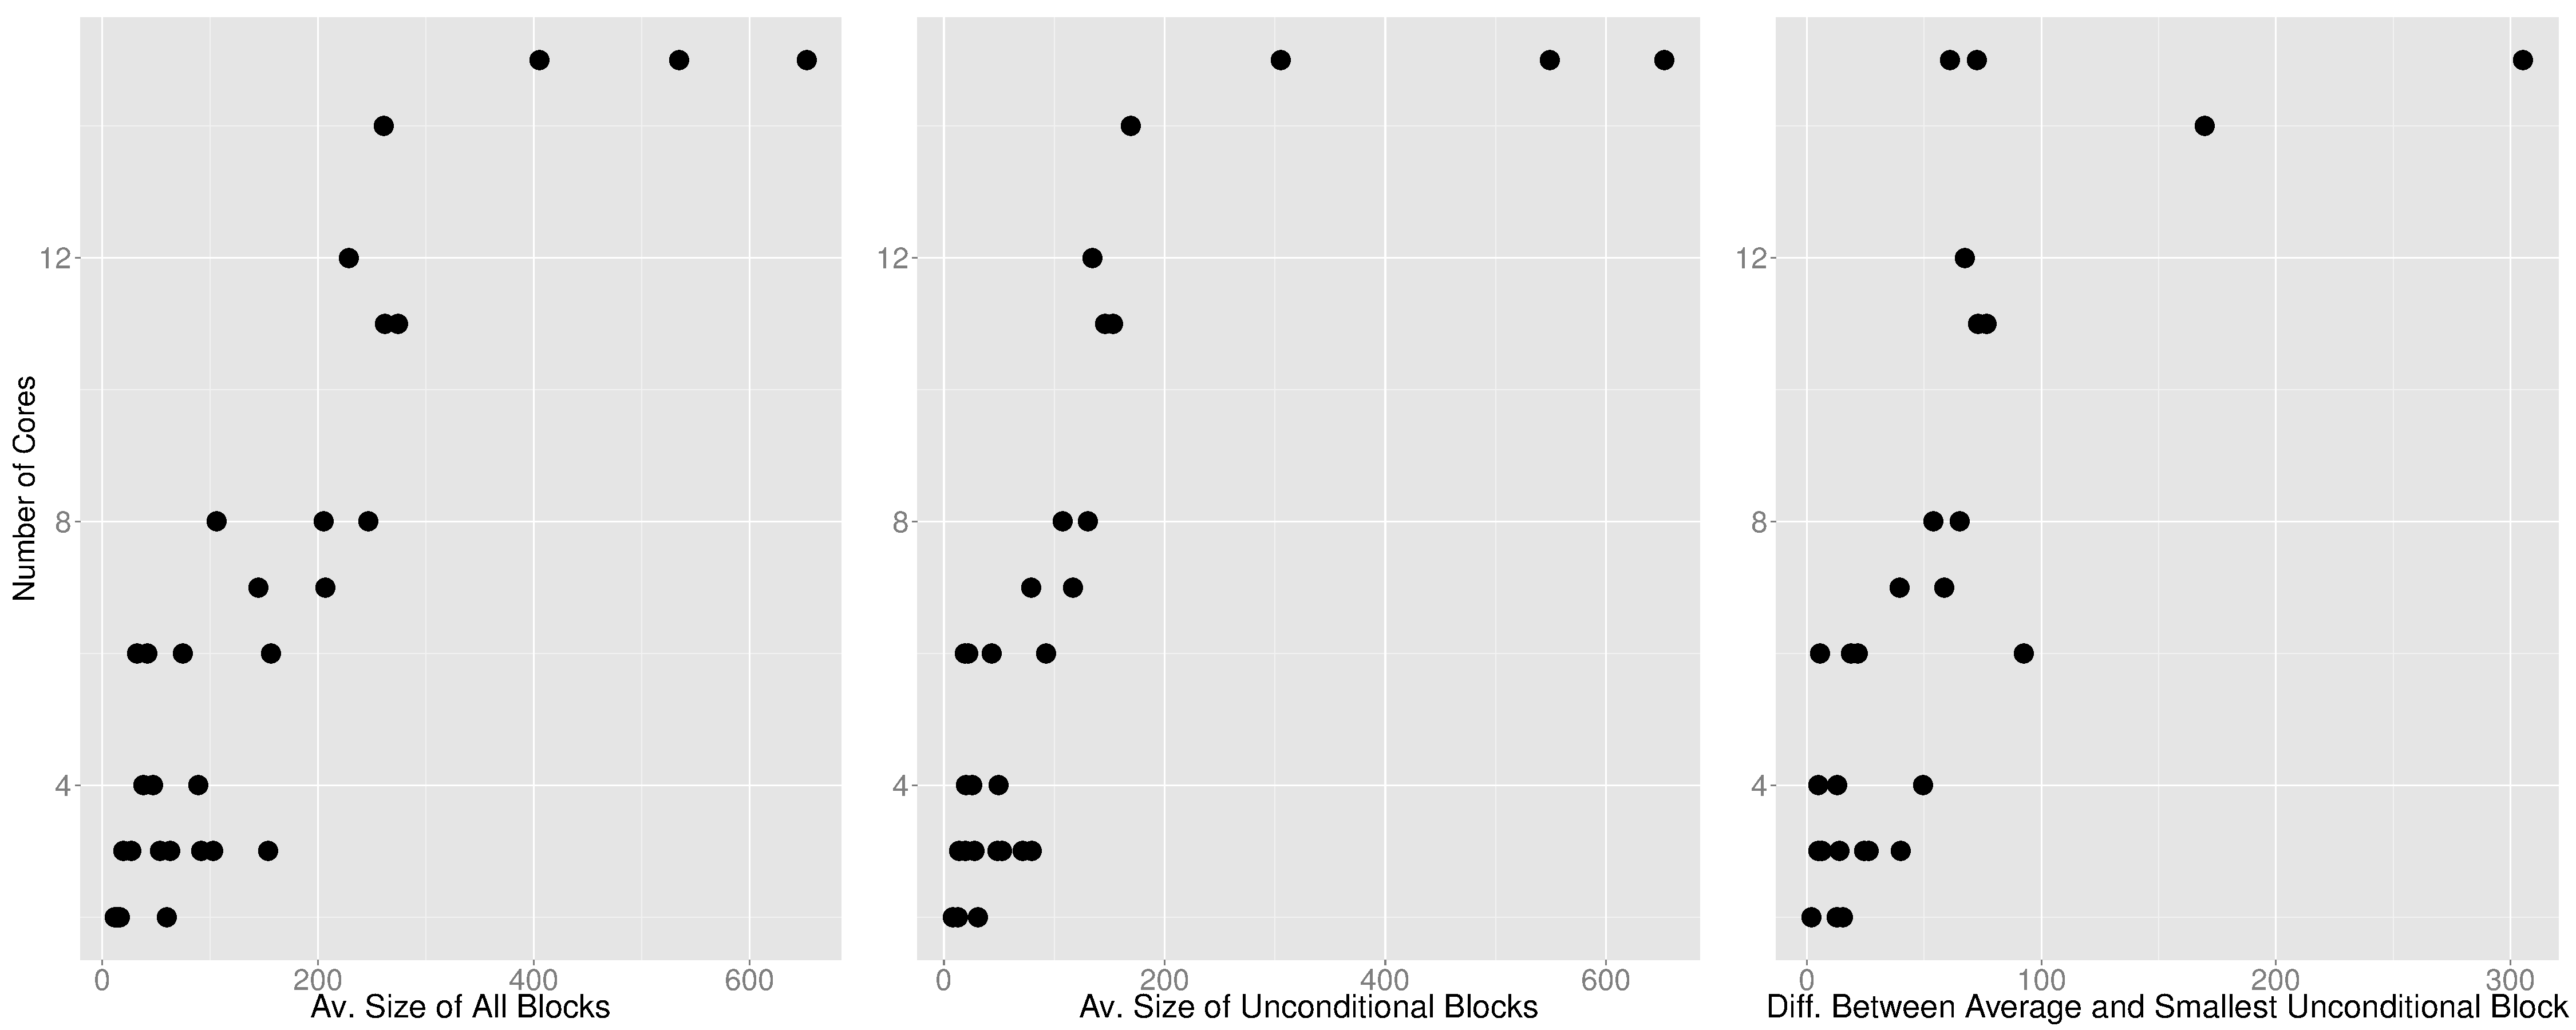
\includegraphics[width=1\textwidth]{streamit-paper/graphics/lineargraphs.pdf}
  \caption{Optimal number of cores in relation to the three highest correlating features. The maximum number of cores plateaus on the right hand side as this is the maximum possible amount.}\label{fig:maxav}
\end{figure}

\subsubsection{Linear Regression Model}
Given that the optimal number of cores highly correlates with a few features, a linear regression is a natural choice to predict the best number of threads.
Figures~\ref{fig:maxav} represent how the first three highest correlating values affect the optimal number of cores for a single-working-thread.
This figure is obtained by finding the best number of cores for the single-working-threaded version of each of the StreamIt benchmarks whilst varying the amount of loop unrolling.
It is important to note that the reason the points in the top right corner appear to converge at 15 cores is due to the fact that no more than 15 cores can be fused.
Overall, Figure~\ref{fig:maxav} shows that StreamIt applications with large unconditionally executed blocks will require large compositions.




%\section{Compiler Optimisation}
%\begin{figure}[t]
\begin{minipage}[t]{0.48\textwidth}
\lstset{language=C,numbersep=4pt,basicstyle=\small}
\begin{lstlisting}
for(int i = 0; i < 1000; i++)
  for(int j = 0; j < 1000; j++)
     for(int k = 0;k < 5; k++)
         a[i][j] = a[i][j] * b[k][j];
\end{lstlisting}
\vspace*{-5mm}
\caption{Example of an inner-most loop which should be completely unrolled.}
\label{lst:small}
\end{minipage}
\hfill
\begin{minipage}[t]{0.48\textwidth}
\lstset{language=C,numbersep=4pt,basicstyle=\small}
\begin{lstlisting}
for(int i = 0; i < 1000; i++)
  for(int j = 0; j < 1000; j++)
      a[i][j] = a[i][j-1] 
                       * b[i][j];
\end{lstlisting}
\vspace*{-5mm}
\caption{Example of a data dependency which can be removed by interchanging the loops.}
\label{lst:dep}
\end{minipage}
\vspace{9mm}
\end{figure}

This section describes optimizations focused on reducing control flow and expanding block sizes which is necessary for high performance as seen in section~\ref{sec:lim_study}.

\subsection{Loop Unrolling}
Loop unrolling is a common optimization used to reduce the overhead of the loop header and to better expose Instruction Level Parallelism (ILP).
When dealing with tightly-knit loops, logical cores may perform poorly due to the fact that they execute many small blocks, thus increasing the Synchronization Cost.
Unrolling loops will both reduce the number of blocks required to execute the loop and increase the size of the blocks, thus reducing the Synchronization Cost and increasing ILP.
For example, the innermost loop in Figure~\ref{lst:small} should be completely unrolled and its outer loop unrolled partially to increase the block size.
There are certain factors which can limit the usefulness of loop unrolling which we examine later on.
In the architecture we evaluate, we may not have more than 32 load or store instructions per block.
Therefore, if we unroll memory intensive loops, we must ensure we do not go above this threshold.
Going above this threshold leads to creating a new block which will put a strain on the branch predictor.
Another issue is that unrolling loops with conditional statements may not help improve the size of the block as the conditional branches might still segment the new blocks.
So we should avoid unrolling such loops.



\subsection{Loop Interchange}
When dealing with nested loops there is one reason we have determined for interchanging the loops.
The case arises when interchanging the loop removes dependencies in the inner-most loop.
The dependency in Figure~\ref{lst:dep} can be removed by interchanging the loops. 
This allows us to unroll the inner loop efficiently, but also remove any kind of dependency between blocks.
Since two blocks from the same loop may execute on different cores, we want to reduce any kind of data dependency, minimizing core communication.

\begin{figure}[t]
     \centering
     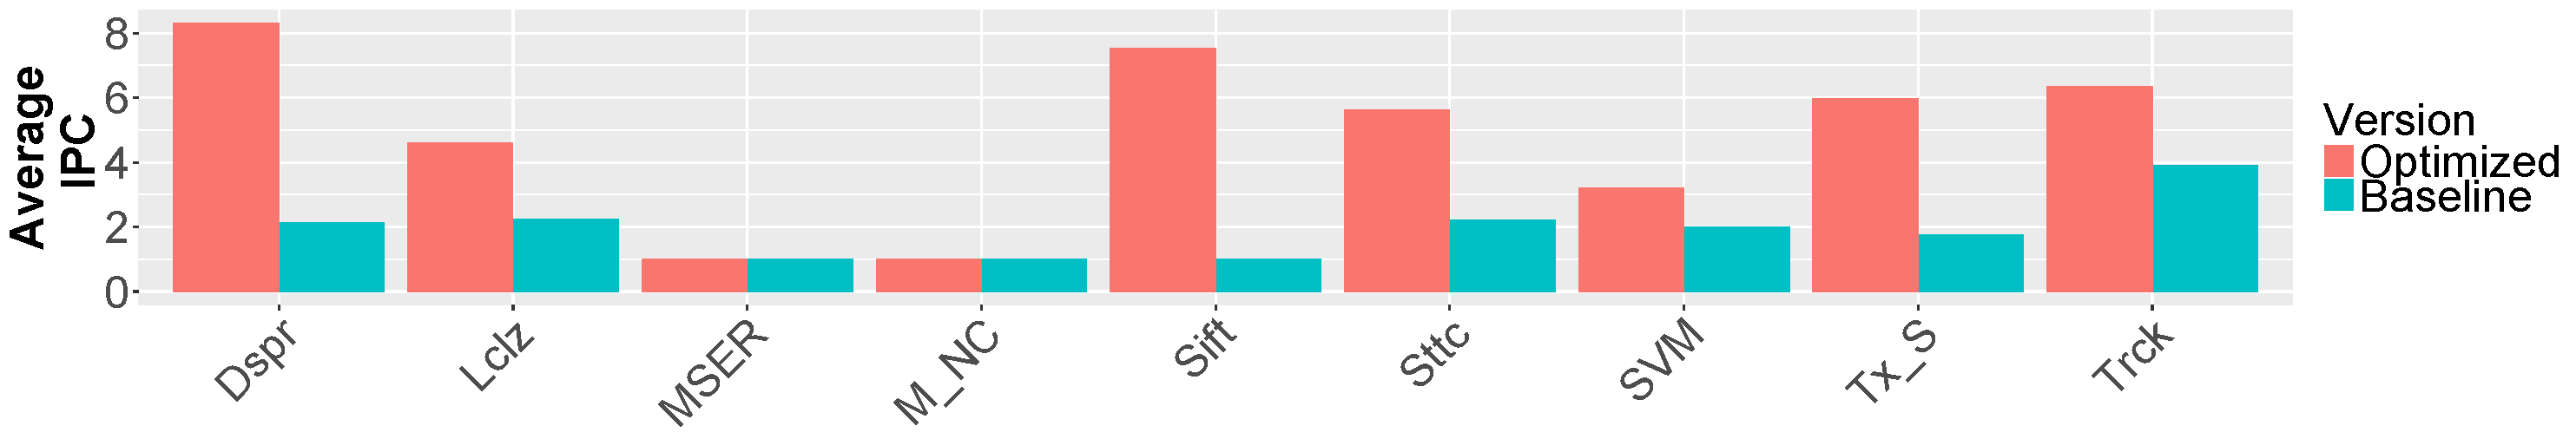
\includegraphics[width=\textwidth]{graphics/Exploration/ipc_comp.pdf}
\vspace*{-8mm}
     \caption{Average IPC using the optimal sized logical-core, with and without optimizations. Higher is better.}
     \label{fig:ipccom}
     \vspace{0.5em}
\vspace{5mm}
    \centering
    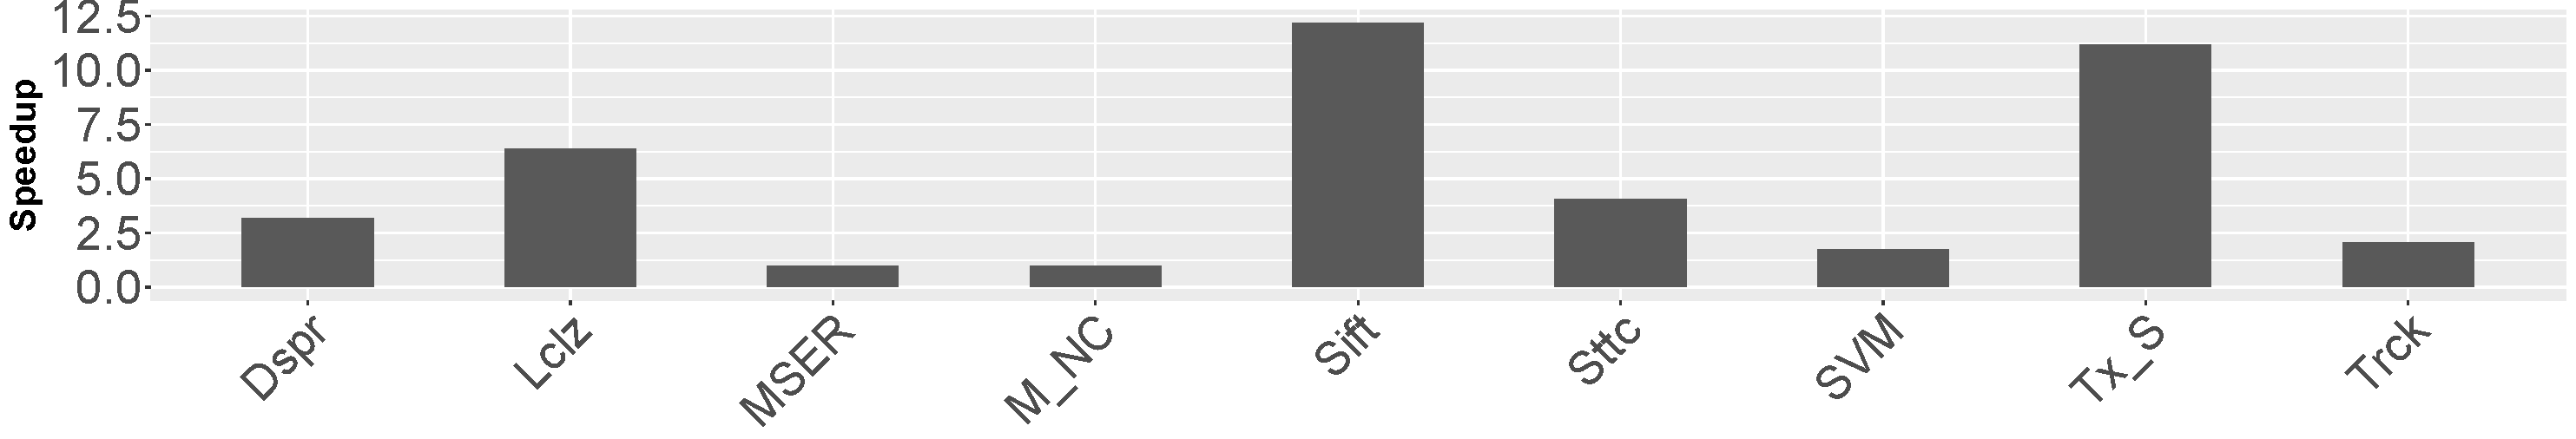
\includegraphics[width=\textwidth]{graphics/Exploration/comp_speed.pdf}
\vspace*{-8mm}
    \caption{Speedup from using code-optimizations over baseline source code using the same optimal sized logical-core.}
    \label{fig:speedcomp}
\vspace{5mm}
\end{figure}

\subsection{Predication and Hyperblock Formation}
EDGE compilers must split blocks whenever control-flow is present~\cite{smith2006edge}.
If a loop contains a conditional statement, the loop body has to be split in two unless if-conversion is applied.
Hyperblock formation aims to reduce branching and increase block size by combining two or more blocks into a single predicated block~\cite{smith2006edge}.
Hyperblocks reduce both synchronization cost and branch prediction requirements as discussed previously.
This is especially important in control-flow intensive loops where unrolling increases the number of conditional statements.

\vspace{5mm}
\subsection{Results}

While the optimizations described above and their tuning would be easy to implement in a compiler, we did not have access to the compiler's source code.
We therefore modified the source code of our benchmarks by manually interchanging or unrolling loops.
In the case of predication and hyperblock formation, we converted simple if-then-else statements into ternary operators whenever possible.
We also tried to reorder statements within the body of a loop to avoid having control flow in the middle of the body.
We then verified that our source code modification had the intended effect by dissembling the binary produced by the compiler.
We modified between 0 and 12 loops depending on the benchmark.

We compare the best static core fusion using the optimized code with the unmodified code, both version compiled with \texttt{-O2}.
Figure~\ref{fig:ipccom} shows the resulting IPC for the baseline case and the optimized benchmarks when run on a core with the optimal number of fused core to maximize performance.
The IPC of the baseline is very low for the majority of the benchmarks which might give the impression that core fusion is rather inefficient.
However, after applying the simple optimizations described above, the average IPC is significantly increased in many cases.

Since optimizations change the total number of instructions, we also show the actual speedup obtained using cycle count in Figure~\ref{fig:speedcomp}.
As we can see, benchmarks \bm{MSER} and \bm{Multi-NCut} do not perform any differently.
This is due to the fact that none of these optimizations can be successfully applied on these benchmarks.
For the other benchmarks we see significant improvements of up to 12$\times$ for \bm{Sift} when the optimizations are applied.

\subsection{Summary}

Overall, this section shows that classical loop transformations can have a large impact on the performance of fused cores.
Without these optimizations, it would be more difficult to motivate the use of core fusion even at a static-level as the IPC does not deviate enough from a single core.


\section{Results}\label{sec:results}
This section describes the performance achieved by the model when predicting the number of threads and core composition to use for each of the StreamIt benchmarks and compares it to the optimal solution found when exploring the space.

\begin{figure}[t]
    \centering
    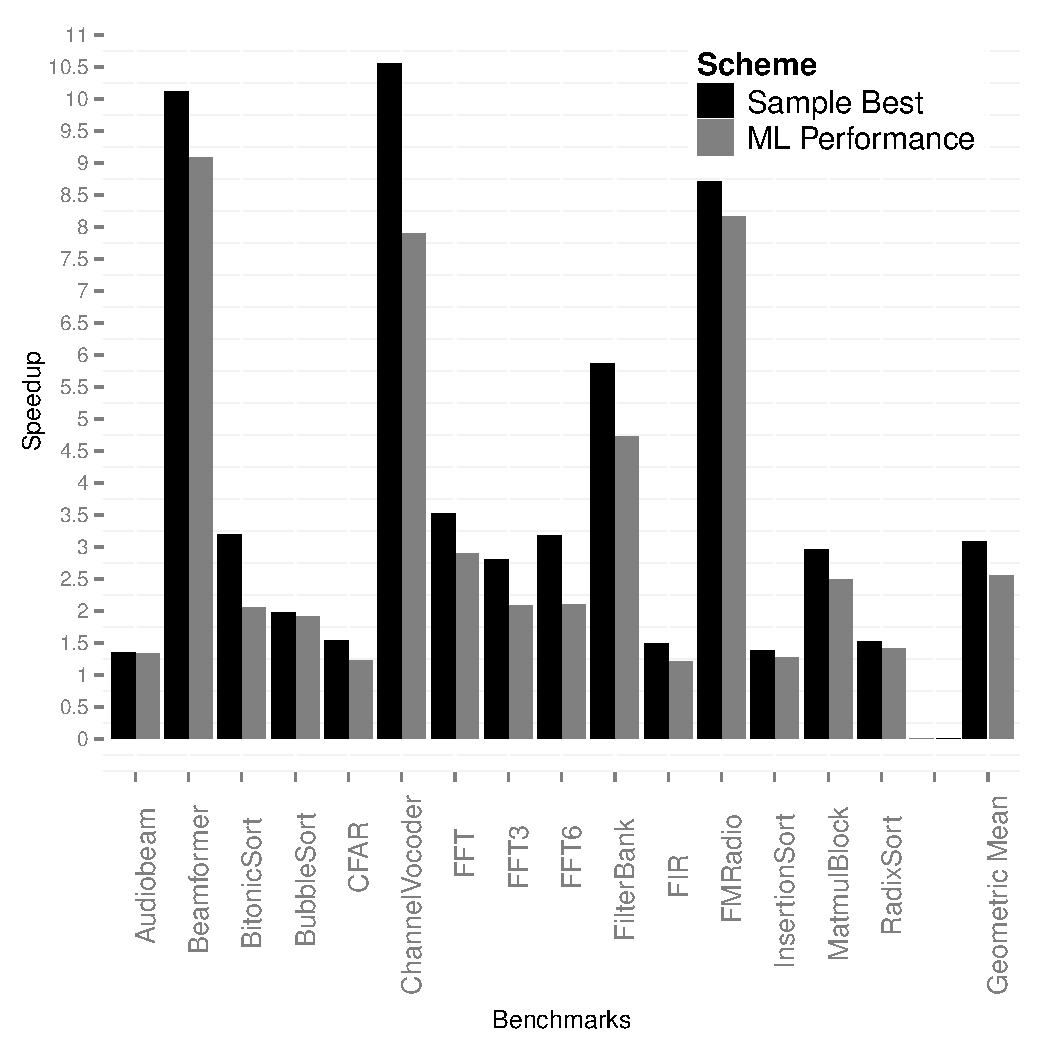
\includegraphics[width=0.7\textwidth]{streamit-paper/graphics/results.pdf}
    \caption{Performance of the machine learning model against the best execution from random sampling. The baseline for the speedup measurement is single core, single thread execution using O2 compiler optimisations. Higher is better.}\label{fig:results}
\end{figure}

\subsection{Machine Learning Model Evaluation Methodology}

Leave-one-out cross-validation is used for testing the linear model.
This means that when testing the model on one application, this application is removed from the training set, the model is trained with the remaining application and finally the model is tested on the application; this process is repeated for each application.
This is standard methodology in the machine-learning community ensuring that the training data is never used for testing.
For the kNN model, the training data consists of all the generated synthetic benchmarks and it is only tested on the real StreamIt applications as they are not used for training.
To obtain the speedup the performance of the machine learning based result are compared to the best from the sample space to running the StreamIt benchmark on a single core, single thread, using O2 compiler optimisations. 

\subsection{Evaluation}

Figure~\ref{fig:results} compares the performance of the machine-learning model and the best performance from the sample space.
As explained in the earlier section, the sampled best is drawn from a sample size of 1,316 combinations of core compositions and thread partitions for each application when possible.
The baseline is the original StreamIt application running with one thread and one core with O2 optimisations on the dynamic multicore processor.
The average speedup obtained through the machine learning model is 2.6 compared to the baseline, this is only 16\% smaller than the average of the best found, which is a speedup of 3.1.
These results are positive as it means the model's results are at least within 16\% of the total best.

As can been seen in Figure~\ref{fig:results} the largest performance penalty resides in the performance of \bench{ChannelVocoder}.
Table~\ref{tab:summary} presents the actual configuration found for the best sampled point and the machine learning model prediction.
Each column represent a different threads and the number in the cell represents the number of core associated with that thread.
For ~\bench{ChannelVocoder} the model predicts only 8 threads rather than the optimal 13.
Referring back to Figure~\ref{fig:threadtrend} and Figure~\ref{fig:overviewhist} from Section~\ref{sec:streamit:dse} \bench{ChannelVocoder} always performs better when adding more threads rather than increasing the size of a core composition.
This is the cause of the performance penalty, for ~\bench{ChannelVocoder} it is more important to allocate a higher number of threads rather than compose cores.
Aside from this case, the machine learning model obtains similar speedups to the best sample.

\begin{table*}[t]
\centering
\resizebox{0.75\textwidth}{!}{\begin{minipage}{0.5\textwidth}
  \small
  \hspace{-5em}
 \begin{tabular} { | l | l | l | l | l | l | l | l | l | l |l| }
    \hline
      & \textbf{1} & \textbf{2} & \textbf{3} & \textbf{4} & \textbf{5} & \textbf{6} & \textbf{7} & \textbf{8} & \textbf{9} & \textbf{10} \\ \hline
    B Audiobeam & 3 & 2 & \cellcolor[gray]{0.3}& \cellcolor[gray]{0.3}& \cellcolor[gray]{0.3}& \cellcolor[gray]{0.3}& \cellcolor[gray]{0.3}& \cellcolor[gray]{0.3}& \cellcolor[gray]{0.3}& \cellcolor[gray]{0.3} \\ \hline 
    M Audiobeam & 2 & 3 & \cellcolor[gray]{0.3}& \cellcolor[gray]{0.3}& \cellcolor[gray]{0.3} & \cellcolor[gray]{0.3}& \cellcolor[gray]{0.3}& \cellcolor[gray]{0.3}& \cellcolor[gray]{0.3}& \cellcolor[gray]{0.3}\\ \hline\hline
    B Beamformer & 1 & 4 & 2 & 4 & 4& \cellcolor[gray]{0.3}& \cellcolor[gray]{0.3}& \cellcolor[gray]{0.3}& \cellcolor[gray]{0.3}& \cellcolor[gray]{0.3} \\ \hline 
    M Beamformer & 6 & 4 & 4& \cellcolor[gray]{0.3}& \cellcolor[gray]{0.3}& \cellcolor[gray]{0.3}& \cellcolor[gray]{0.3}& \cellcolor[gray]{0.3}& \cellcolor[gray]{0.3}& \cellcolor[gray]{0.3} \\ \hline\hline
    B BitonicSort & 3 & 2 & 2 & 2 & \cellcolor[gray]{0.3}& \cellcolor[gray]{0.3}& \cellcolor[gray]{0.3}& \cellcolor[gray]{0.3}& \cellcolor[gray]{0.3}& \cellcolor[gray]{0.3}  \\ \hline
    M BitonicSort & 1 & 2 & 2 & 1 & 2 & 2 & 2 & \cellcolor[gray]{0.3}& \cellcolor[gray]{0.3}& \cellcolor[gray]{0.3} \\ \hline\hline
    B BubbleSort & 3 & 3& \cellcolor[gray]{0.3} & \cellcolor[gray]{0.3} & \cellcolor[gray]{0.3}& \cellcolor[gray]{0.3}& \cellcolor[gray]{0.3}& \cellcolor[gray]{0.3}& \cellcolor[gray]{0.3}& \cellcolor[gray]{0.3} \\ \hline
    M BubbleSort & 2 & \cellcolor[gray]{0.3} & \cellcolor[gray]{0.3} & \cellcolor[gray]{0.3} & \cellcolor[gray]{0.3}& \cellcolor[gray]{0.3}& \cellcolor[gray]{0.3}& \cellcolor[gray]{0.3}& \cellcolor[gray]{0.3}& \cellcolor[gray]{0.3} \\ \hline\hline
    B CFAR & 3 & 2 & \cellcolor[gray]{0.3} & \cellcolor[gray]{0.3} & \cellcolor[gray]{0.3}& \cellcolor[gray]{0.3}& \cellcolor[gray]{0.3}& \cellcolor[gray]{0.3}& \cellcolor[gray]{0.3}& \cellcolor[gray]{0.3} \\ \hline 
    M CFAR & 2 & 2  & 1  & 2 & \cellcolor[gray]{0.3}& \cellcolor[gray]{0.3}& \cellcolor[gray]{0.3}& \cellcolor[gray]{0.3}& \cellcolor[gray]{0.3}& \cellcolor[gray]{0.3} \\ \hline\hline
    B ChannelVoc.& 4 & 1 & 1 & 1 & 1 & 1 & 2 & 1 & 1 & 1 \\ \hline 
    M ChannelVoc.& 2 & 2 & 1 & 2 & 2& 2 & 2& \cellcolor[gray]{0.3}& \cellcolor[gray]{0.3}& \cellcolor[gray]{0.3} \\ \hline\hline
    B FIR & 3 & 2 &\cellcolor[gray]{0.3}&\cellcolor[gray]{0.3}&\cellcolor[gray]{0.3}&\cellcolor[gray]{0.3}&\cellcolor[gray]{0.3}&\cellcolor[gray]{0.3}&\cellcolor[gray]{0.3}&\cellcolor[gray]{0.3}\\ \hline
    M FIR & 2 & 2&\cellcolor[gray]{0.3}&\cellcolor[gray]{0.3}&\cellcolor[gray]{0.3}&\cellcolor[gray]{0.3}&\cellcolor[gray]{0.3}&\cellcolor[gray]{0.3}&\cellcolor[gray]{0.3}&\cellcolor[gray]{0.3}\\ \hline\hline
    \end{tabular}
  \end{minipage}	\hfill
  \hspace{1em}
\begin{minipage}{0.5\textwidth}

	 \begin{tabular} { | l | l | l | l | l | l | l |}
    \hline
      & \textbf{1} & \textbf{2} & \textbf{3} & \textbf{4} & \textbf{5} & \textbf{6}  \\ \hline

	B FFT & 3 & 3 & 5 & \cellcolor[gray]{0.3}& \cellcolor[gray]{0.3}& \cellcolor[gray]{0.3} \\ \hline
    M FFT & 6& 5 & 2& \cellcolor[gray]{0.3}& \cellcolor[gray]{0.3}& \cellcolor[gray]{0.3}  \\ \hline\hline
    B FFT3 & 3 & 2 & 2& \cellcolor[gray]{0.3}& \cellcolor[gray]{0.3}& \cellcolor[gray]{0.3} \\ \hline 
    M FFT3 & 3 & 2 & 3 & 3& 3& 3 \\ \hline\hline
    B FFT6 & 7 & 8& \cellcolor[gray]{0.3}& \cellcolor[gray]{0.3}& \cellcolor[gray]{0.3}& \cellcolor[gray]{0.3}\\ \hline
    M FFT6& 14 & \cellcolor[gray]{0.3}& \cellcolor[gray]{0.3}& \cellcolor[gray]{0.3}& \cellcolor[gray]{0.3}& \cellcolor[gray]{0.3} \\ \hline\hline
    B FilterBank & 4 & 5 & 6& \cellcolor[gray]{0.3}& \cellcolor[gray]{0.3}& \cellcolor[gray]{0.3} \\ \hline
    M FilterBank & 4 & 5 & \cellcolor[gray]{0.3} & \cellcolor[gray]{0.3}& \cellcolor[gray]{0.3}& \cellcolor[gray]{0.3}\\ \hline\hline
    B FMRadio & 7 & 6 & \cellcolor[gray]{0.3}& \cellcolor[gray]{0.3}& \cellcolor[gray]{0.3}& \cellcolor[gray]{0.3}\\ \hline
    M FMRadio & 7 & 4 & \cellcolor[gray]{0.3} & \cellcolor[gray]{0.3}& \cellcolor[gray]{0.3}& \cellcolor[gray]{0.3} \\ \hline\hline
    B InsertionSort & 3 & 2& \cellcolor[gray]{0.3}& \cellcolor[gray]{0.3}& \cellcolor[gray]{0.3}& \cellcolor[gray]{0.3} \\ \hline
    M InsertionSort & 3 & \cellcolor[gray]{0.3}& \cellcolor[gray]{0.3}& \cellcolor[gray]{0.3}& \cellcolor[gray]{0.3}& \cellcolor[gray]{0.3}\\ \hline\hline
    B MatmulBlock & 3 & 4 & 6 & 2 & \cellcolor[gray]{0.3} & \cellcolor[gray]{0.3}\\ \hline
    M MatmulBlock & 4 & 4 & \cellcolor[gray]{0.3}& \cellcolor[gray]{0.3}& \cellcolor[gray]{0.3}& \cellcolor[gray]{0.3}\\ \hline\hline
    B RadixSort & 3 & 3& \cellcolor[gray]{0.3}& \cellcolor[gray]{0.3}& \cellcolor[gray]{0.3}& \cellcolor[gray]{0.3}\\ \hline
    M RadixSort & 2 & 2& \cellcolor[gray]{0.3}& \cellcolor[gray]{0.3}& \cellcolor[gray]{0.3}& \cellcolor[gray]{0.3}\\ \hline
    
 \end{tabular}
  \end{minipage}}
  \caption{Number of Threads and Cores used for Best of Sample Space and Machine Learning Model.}\label{tab:summary}

\end{table*}

 \subsection{Summary}

This section has demonstrated that it is possible to build a machine-learning model that achieves high level of performance using simple source code static features.
In many applications, the model even comes very close to the best from the sampled space, showing that the features used by the model contain enough information to inform the model about the best decision.

\vspace{5mm}


%\section{Related Work}
%\label{sec:related}
%\paragraph{Dynamic Multicore Processors}

DMPs such as CoreFusion~\cite{ipek2007CoreFusion} differentiate themselves to EDGE based DMPs on their Instruction Set Architecture (ISA).
CoreFusion uses a CISC/RISC based architecture which limits the degree of scalability (fusion), whereas EDGE based DMPs have shown promising scalability~\cite{kim2007composablelight, sibi2014}.
Other types of DMPs such as WidGET~\cite{Watanabe2010Widget} and Sharing Architecture~\cite{zhou2014sharingarch} present a fine-grain level of composition.
In these two architectures, cores can be created out of different components on the processor, including ALUs, floating point units and memory units.
This differs from CoreFusion and EDGE where a logical core is composed out of a set of physical cores.
This fine-grained composition can allow for even more optimisation but it increases the complexity of the problem.

\paragraph{Core Configuration}

Little work has been done on automatically determining the correct core composition for a given application.
The work conducted in~\cite{ipek2007CoreFusion,kim2007composablelight} manually configure their processors before running benchmarks.
In~\cite{santos2013nocdmc} they use information provided by the application to determine how to reconfigure some components of the processor.
This initial information then assists the rest of the reconfiguration, this process still requires input from the programmer though.
Therefore we present a novel method for automating the choice of core composition.  

\vspace{2mm}
\paragraph{Streaming Programming Languages}

There exist streaming languages that target different architectures.
For example Brook~\cite{buck2004brook} is designed to be used on GPUs and WaveScript for embedded systems~\cite{newton2008wavescript}.
These languages present different constructs to StreamIt, in particular they lack the graph oriented constructs. 
Lacking such constructs make these languages less attractive for tiled processors.

\paragraph{Partitioning StreamIt on multicore chip}

Previous work on scheduling streaming applications onto DMPs or heterogenous multicore chips focuses on finding mathematical ways of partitioning the graph onto the chip ~\cite{carpenter2009streammap,kudlur2008orchestratingstreamprog}.  
In Carpenter et al.'s work~\cite{carpenter2009streammap} they restrain themselves to partitioning a StreamIt application maintaining connectedness.
Connectedness can be defined as a subgraph where the filters are connected. 
This restriction reduces the number of potential partitions that can be generated by their algorithm and will put TLP in favour of ILP. 
Kudlur et al. in~\cite{kudlur2008orchestratingstreamprog} choose to represent the partitioning problem as an integer linear programming problem.
They start by fissionioning stateless filters to obtain the optimal load balance across all cores and assign the filters to a core using a modulo scheduler.
Farhad et al. also use integer linear programming in~\cite{farhad2012streamilp} to schedule StreamIt programs on multicore.
They profile the communication costs of the streaming programs by running the program using different multicore allocations and feed that information into their integer linear programming model.

\paragraph{Machine Learning} Using a machine learning model to partition StreamIt programs was previously explored in the work of Wang et al. in ~\cite{wang2013partitionstreamit}.
They use a k nearest neighbor model to determine the perfect partitioning of a StreamIt program for a multicore system. 
The features we extracted using correlation analysis are similar to those presented in the work of ~\cite{wang2013partitionstreamit}.
Unlike our work their model is used to find ways of fusing and fissioning filters to discover a new graph that can then be mapped onto a multicore system.



\section{Conclusion}\label{sec:conclusion}
In this paper we presented the problem of partitioning both software and hardware for a Dynamic Multicore Processor.
We analysed a set of streaming workloads based on StreamIt, extracting features which highly influence both the required number of threads and core composition.
Using this data we introduced a machine learning model which is able to determine how many threads a StreamIt application needs and pick an appropriate chip topology.
The model predicts configurations close to the performance of the best design points from the sampled space.
By automating the decision of core composition we motivate the use of DMPs for accelerating applications without any involvement from the programmer.


%\section*{Acknowledgements}
%\label{sec:acknowledgements}
%This work has been supported by Microsoft Research through its PhD Scholarship Programme and has made use of the resources of the Edinburgh Compute and Data Facility (ECDF)~\cite{ecdf}.


%\acks
%
%Acknowledgments, if needed.
%\balance
%\bibliographystyle{abbrvnat}
%\bibliography{references}


%                       Revision History
%                       -------- -------
%  Date         Person  Ver.    Change
%  ----         ------  ----    ------

%  2013.06.29   TU      0.1--4  comments on permission/copyright notices


\newcommand{\bm}[1]{\textit{#1}}
%test
% Copyright
%\setcopyright{none}
%\setcopyright{acmcopyright}
%\setcopyright{acmlicensed}
%\setcopyright{rightsretained}
%\setcopyright{usgov}
%\setcopyright{usgovmixed}
%\setcopyright{cagov}
%\setcopyright{cagovmixed}
% DOI
\setlength{\textfloatsep}{0.1cm}

\chapter{Dynamic runtime adaptation for efficient execution}\label{chp:cases}


The previous chapter explored how static ahead-of-time configuration of a dynamic multicore processor (DMP) can improve the performance of multi-threaded streaming applications and showed how a mix of core and thread partitioning leads to optimal performance.
Static ahead-of-time configurations can improve the overall performance of programs, however they cannot adapt themselves to exploit the different phases a program may have.
A program phase can be used to describe multiple concepts, for example regions of code that exhibit different Instruction per cycle (IPC) performances, or variations of instruction mixes.
When programs exhibit different phases of IPC, this can result in situations where composing multiple cores may be an inefficient solution, thus wasting resources.
Chapter~\ref{chp:streamit} explored multi-threaded applications yet core composition is designed to improve the performance of single threaded applications~\cite{ipek2007CoreFusion} as it has become harder to improve performance for these types of applications.
Therefore this chapter focuses on how a DMP can reconfigure itself at runtime to exploit phases of a set of single-threaded applications.

%Core composition is a technique that allows multiple cores to work on a single thread, allowing a DMP to improve the performance of single threaded applications.
As previously discussed the reconfiguration can happen ahead of time, especially when programs do not have a high variation in IPC.
However, programs can benefit from different adaptations of the hardware at different phases of its execution.
Some programs may have phases that feature high IPC whilst other phases do not perform any better on a set of composed cores.
Therefore, for programs that feature many phases, runtime reconfiguration is necessary to ensure efficient use of a DMP.

Whilst optimising for speed is an important method of evaluating a DMP, the ability to reconfigure the processor allows the hardware to adapt to different performance profiles.
For example, a DMP can reconfigure itself at runtime to maximise energy efficiency, instead of only focusing on speed.
Yet, whilst being able to adapt to different profiles is an attractive feature, determining when to reconfigure the processor is a challenging task for programmers.
It is also difficult for compilers to determine when to compose cores without profiling information as core composition is sensitive to branch prediction and memory dependencies that may only be determined at runtime.% relying on programmers to determine when to reconfigure the processor is a challenging task. 
Automating the decision of when to compose cores allows the programmer to solely focus on the software rather than decide when to modify the hardware.

The previous chapter used streaming applications to explore how partitioning a DMP can improve performance.
Through partitioning, the different computation phases of the streaming programs are essentially divided amongst those threads.
This chapter explores a set of single-threaded C applications, where phases cannot be isolated into different threads.
A domain that features different phases of computations and is also prominent in the embedded space is image and vision recognition.
Since these applications are often designed as software pipelines, they present different phases throughout their execution, and thus are an interesting case for dynamic adaptation of a DMP.

The chapter starts with an explanation of the theoretical limitations of core composition and what can be expected in terms of performance.
Then the next section discusses the necessity of fine grained loop optimisations as they have a large impact on performance when composing cores.
Using the San Diego Vision Benchmark Suite~\cite{sdvbs} (SD-VBS) as a use case, the chapter demonstrates that programs exhibit various phases with different amounts of IPC.
This is followed by a limit study on the potential for decreasing energy consumption while maintaining performance when adapting the number of cores for each program phase.
The results show that using dynamic core composition can save up to 42\% on average while maintaining the same level of performance as a fixed number of cores.
The issue of latency introduced by reconfiguring the system is then discussed and its influence on the impact of core composition is explored.
Finally, a linear regression model that predicts the optimal number of cores per phase for reducing energy consumption while maintaining performance is generated.
This practical model leads to an average of 37\% saving in energy with no performance loss.

To summarise, the contributions are:
\vspace{-1em}
\begin{itemize}
\item Analysis of the limits of core composition using an analytical model.
\vspace{-1em}
%\item A study of the loop optimisations required to ensure efficient use of core composition.
%\vspace{-2.5em}
\item An in-depth comparison of static and dynamic core composition schemes on the San Diego Vision Benchmark Suite.
\vspace{-1em}
\item Evidence that core composition has the potential to offer a large reduction in energy savings.
\vspace{-1em}
\item An analysis of how the overhead of reconfiguring the processor can affect the potential benefits of core composition.
\vspace{-1em}
\item A demonstration that a linear-regression based model can predict the number of cores to fuse for different program phases.
\end{itemize}


%\section{Dynamic Multicore Processor}\label{sect:background}
%\paragraph{Dynamic Multicore Processor} DMPs contain hardware which can be modified post fabrication.
Mitall's survey ~\cite{MittalSurv2016} defines three types of modifiable resources: the core count~\cite{ipek2007CoreFusion}, number of resources that each core has~\cite{Homayoun3DPooling2012} and micro-architectural features~\cite{fallinhetblock2014,BauerRSE08,tavanaElastic}.
In our paper we focus on DMPs that modify the core count.

\paragraph{EDGE ISA} We assume a DMP similar to TFlex~\cite{kim2007tflex} using an Explicit Data Graph Execution~\cite{burger04edge} (EDGE) instruction set architecture (ISA).
EDGE ISAs encode dependencies between instructions at the ISA level.
Code is organised as blocks of instructions where all instruction communication is local to the block~\cite{smith2006edge}.
Each block has a single entry point but may have multiple exits.
This enables the architecture to dispatch blocks speculatively, with low overhead~\cite{putnam2010e2,kim2007tflex}, therefore, increasing exploitation of ILP.

 \begin{figure*}[t]
 \center
 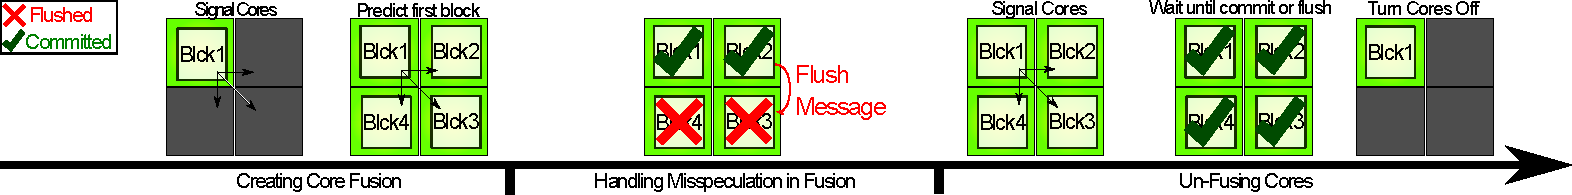
\includegraphics[width=1\textwidth]{cases-paper/graphics/background/proc_test.pdf}
\vspace*{-5mm}
 \caption{Core Fusion Mechanisms for our EDGE-based architecture.}\label{fig:dmp}
\vspace{-5mm}
 \end{figure*}
\paragraph{Core Fusion} 
Core Fusion is achieved by fusing a set of \textit{physical} cores to create larger \textit{logical} cores.
This does not modify the physical structure of the chip, instead it provides a unified view of a group of physical cores to the software.
For example, fusing two cores generates a logical core with twice the amount of execution units, register files and L1 cache.
Fusion is a dynamic modification and may occur during the execution of a program to better fit the workload.
Unlike traditional CMPs, fused cores will operate on the same thread and attempt to extract Instruction Level Parallelism (ILP) rather than Thread Level Parallelism (TLP)~\cite{micolet2016dmpstream,pricopi2012bahurupi}.
Figure~\ref{fig:dmp} shows the different stages and mechanisms of core fusion for a four core system.
When creating a new core fusion a master core informs all other cores about the fusion and sends the predicted next block address to the next available fused core.
When a core mis-predicts a branch in a fusion, it informs the other cores which flush any younger blocks.
When un-fusing, the master core informs the other cores, which then commit or flush their blocks and power down while the master core continues to fetch and execute blocks from the thread.
The extra hardware required to support dynamic reconfiguration is very minimal~\cite{kim2007tflex} since most of the machinery already in place can be reused such as the cache coherence protocol when fusing and un-fusing the cores.
We discuss this in further detail in Section~\ref{sec:setup}.


\section{Motivation}\label{sec:motivation}
This section motivates the use of dynamic core composition and its impact on performance and energy.
It also shows that loop optimisations have a significant performance impact when fusing cores.
As instructions per cycle (IPC) is a commonly used method of measuring performance, it is used throughout this chapter.

\subsection{Dynamic Core Composition}
\begin{figure}[t]
    \centering
    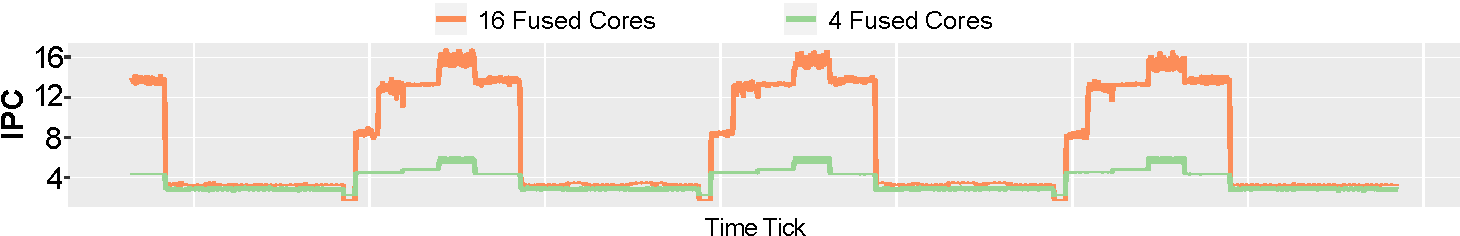
\includegraphics[width=\textwidth]{cases-paper/graphics/motivation/disp_opt_4_16_3.pdf}
    \caption{IPC of a typical benchmark (Disparity from SD-VBS) when executing on a composition of 4 or 16 core processor.} 
    \label{fig:disp_ex}
	\vspace{-2em}
\end{figure}

%\begin{figure}[t]
%    \centering
%    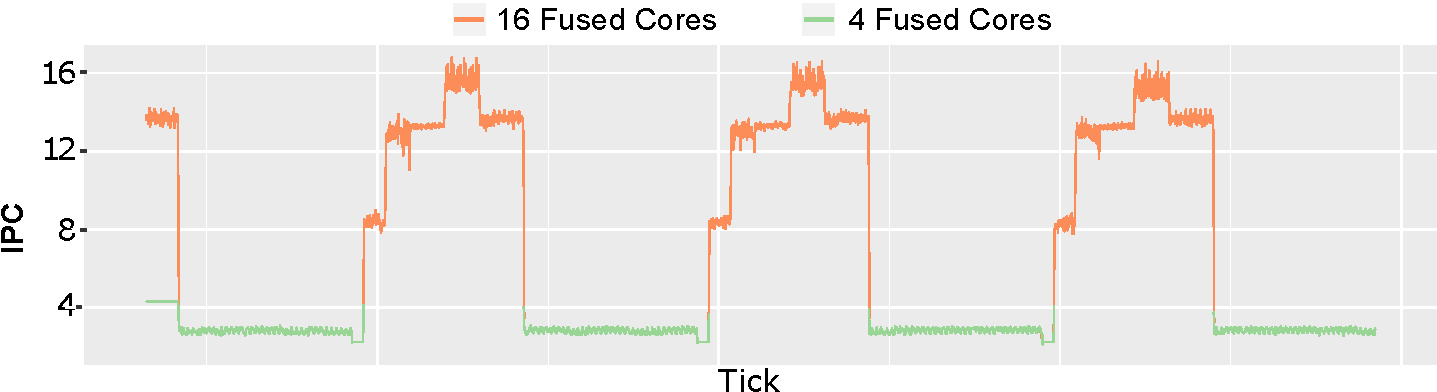
\includegraphics[width=\textwidth]{cases-paper/graphics/motivation/motiv3merge.pdf}
%    \caption{Example of ideal switching between 4 and 16 cores on a DMP for the Disparity benchmark.} 
%    \label{fig:ideal_switch}
%\vspace{2em}
%\end{figure}


\lstset{
	backgroundcolor=\color{lbcolor},
	tabsize=2,
	rulecolor=,
	language=matlab,
        basicstyle=\tiny,
        upquote=true,
        aboveskip={1\baselineskip},
        columns=fixed,
        showstringspaces=false,
        extendedchars=true,
        breaklines=true,
        prebreak = \raisebox{0ex}[0ex][0ex]{\ensuremath{\hookleftarrow}},
        frame=single,
        showtabs=false,
        showspaces=false,
        showstringspaces=false,
        identifierstyle=\ttfamily,
        keywordstyle=\color[rgb]{0,0,1},
        commentstyle=\color[rgb]{0.133,0.545,0.133},
        stringstyle=\color[rgb]{0.627,0.126,0.941},
		numbers=left,
}


Previous work in core composition focuses on delivering performance improvements \cite{ipek2007CoreFusion,kim2007tflex} and demonstrates how to predict static core fusion~\cite{micolet2016dmpstream}.
A static ahead of time composition fuses cores into a single composition and executes a thread on it.
As evident from this prior work, core composition improves the performance of the program by maximising speed.
However, as will be shown a static ahead of time core compositions may not be the perfect match for all situations.

\begin{figure}[t]
\lstset{language=C,numbersep=4pt}
\begin{center}
\begin{lstlisting}
for(i=0; i<nr; i++) {
	for(j=0; j<nc; j++) {
		a = retSAD->data[i*retSAD->width+j];
		b = minSAD->data[i*minSAD->width+j];
		if(a<b) {
			minSAD->data[i*minSAD->width+j] = a;
			retDisp->data[i*retDisp->width+j] = level;
		}
	}
}

\end{lstlisting}
\end{center}
\vspace{-1em}
\captionof{lstlisting}{Disparity code that causes low IPC.}
\label{lst:low_ipc}
\end{figure}

\begin{figure}[t]
\lstset{language=C,numbersep=4pt}
\begin{center}
\begin{lstlisting}
nr = SAD->height;
nc = SAD->width;

for(i=0; i<nc; i++)
	subsref(integralImg,0,i) = subsref(SAD,0,i);

for(i=1; i<nr; i++)
	for(j=0; j<nc; j++) 
		subsref(integralImg,i,j) = subsref(integralImg, (i-1), j) + subsref(SAD,i,j);
for (i = 0; i < nr; i++)
	for (j = 1; j < nc; j++)
		subsref(integralImg, i, j) = subsref(integralImg, i, (j - 1)) + subsref(integralImg, i, j);

\end{lstlisting}
\end{center}
\vspace{-2em}
\captionof{lstlisting}{Disparity code that leads to high IPC.}
\label{lst:high_ipc}
\end{figure}

Applications often feature different phases of IPC due to varying loop patterns.
To illustrate this Figure~\ref{fig:disp_ex} plots the IPC performance variation over the execution of the \bm{Disparity} Benchmark from the San-Diego Vision Benchmark Suite (SD-VBS)~\cite{sdvbs} on core compositions of sizes 4 and 16 respectively.
IPC is a natural method of evaluating the performance of a core composition as increasing the size of the composition can lead to a higher amount of instructions executing per cycle.
In this Figure, the x-axis tick represents a certain number of blocks (see Chapter~\ref{chp:Background} Section~\ref{sec:edge_isa}) that are committed rather than being a measure of time in cycles.
This is why the high IPC phases for both compositions appear to last the same length of time even though the 16 core-composition executes the blocks faster.
The reason why the number of blocks committed is used as a measurement of time is due to the fact that the number of blocks necessary to execute a program are independent of the size of a core-composition.
On 4 cores, the performance oscillates between an IPC of 2 and 6 depending on the phase while on 16 cores the IPC can be as high as 16.

As can be seen in Figure~\ref{fig:disp_ex}, both the 4 and 16 core compositions share the same IPC when it comes to the low IPC phase.
Listings~\ref{lst:low_ipc} and~\ref{lst:high_ipc} represent parts of the source code that lead to the low IPC behaviour and high IPC behaviour respectively.
In listing~\ref{lst:low_ipc}, the compiler generates smaller blocks due to the control flow, which often leads to low IPC performance as will be explained later on in Section~\ref{sec:lim_study}.
In these situations, using a large core composition will not improve performance, which is why both the 4 and 16 core-composition share the same IPC.
However the code in listing~\ref{lst:high_ipc} can be unrolled and thus a high amount of IPC can be extracted.
In a situation where the objective of the programmer is to maximise speed, without dynamic reconfiguration of the DMP, a static 16 core-composition will have to be used.
%Get actual energy estimations ot make this more clear
If the static 16 core composition is used, the DMP consumes 4 times as much energy to execute the low IPC phases compared to the 4 core-composition.
This is due to the fact that it uses 4 times as many resources as the 4 core composition to achieve the same performance.
Thus, the static 16 core composition is considered energy inefficient during half the execution of the program.

On the other hand, if the DMP is reconfigured at runtime, the core composition can switch to 4 cores when in the low-IPC phase to save on energy and switch to the 16 core composition when in the high IPC phase to maximise speedup.
In this situation, runtime reconfiguration allows to maximise speed whilst being energy efficient; a goal that cannot be achieved via static ahead of time configurations.

%Maybe, just maybe, add a graph showing how the size of the blocks change (need data on this).
\subsection{Code Optimisations}

When cores are composed they execute blocks of instructions in parallel on each physical core in the core composition.
%Having multiple cores in a composition can increase the amount of block level parallelism (BLP) that can be extracted out of a program.
%A high amount of BLP leads to high IPC as each core in the composition executes their block in parallel.
In order to obtain the best performance from an application, large blocks must be generated as this leads to a higher IPC on the composition as described in Chapter~\ref{chp:streamit} Section~\ref{sec:streamit:dse}.
In a nutshell, larger blocks reduce the amount of time taken to fetch blocks for all the physical cores in the composition, thus improving performance.
Thus, optimisations that maximise block size will positively affect the performance of compositions.
This includes optimisations such as aggressive loop unrolling, inlining and replacing conditional statements with either software predication or architecture-level predication.
These optimisations are well known and do not require any structural modifications of the program.

\begin{figure}[t]
    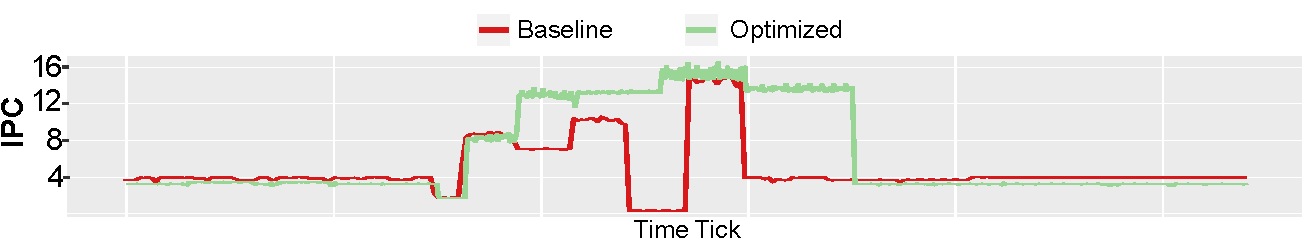
\includegraphics[width=\textwidth]{cases-paper/graphics/motivation/code_opt_3.pdf}
    \caption{Impact of loop transformations on fused cores for the Disparity benchmark.} 
    \label{fig:compmotiv}
\vspace{1em}
\end{figure}

Figure~\ref{fig:compmotiv} illustrates the impact of applying loop transformations on the \bm{Disparity} benchmark compared to a standard compiler not specifically tuned for the EDGE architecture.
In this case, the two main transformations are loop unrolling and loop interchanging.
The Figure shows the IPC performance of a 16 core composition with and without optimisations.
For example, in Listing~\ref{lst:high_ipc}, the nested loop at lines 14 to 16 has a data dependency between iterations; switching the for loop headers can get rid of the dependency.
As can be seen, the impact of these transformations can be large, leading to an 12x improvement on IPC.
Figure~\ref{fig:compmotiv} shows that the optimisations allow the core-composition to sustain a high IPC phase longer than without the optimisations.
Longer high IPC phases also means that the DMP will require less switching between core compositions, thus incurring less of a reconfiguration penalty.
However, it also demonstrates that not all of the code in a program can be optimised, as the low-IPC phases do not change.
More details about the loop transformations are given in section~\ref{sec:opt} but this example illustrates the need for careful tuning of the compiler to achieve high performance on such an architecture.

%Find some citation for this
\subsection{Knowing when and how to reconfigure the processor}

Figure~\ref{fig:disp_ex} motivates the use of runtime reconfiguration to ensure that DMP can improve the performance of single threaded applications efficiently by minimising energy consumption.
Figure~\ref{fig:compmotiv} shows how modifying loops affects the performance in terms of IPC for a core composition.
Using an API, a programmer could inform the hardware when to reconfigure by using specific functions or pragmas similar to OpenMP~\cite{openmp} or OpenCL~\cite{opencl}.
Whilst this may be a viable approach to applying runtime reconfiguration, automating the decision process is a better option.

Automating the process of reconfiguring the processor enables two advantages compared to manually determining when to reconfigure the processor.
The first advantage is that it removes the responsibility from the programmer: an automated runtime reconfiguration system can detect phases and adapt to them accordingly, using information gathered from previous traces.
Second, if ever the program is modified, this may require new profiling information to be generated to ensure that manual reconfiguration calls are correct.
If the reconfiguration is automated, then it can adapt automatically to any changes made to the source code.

\paragraph*{Summary}
This section has shown that programs exhibit phases with various amount of ILP available.
A DMP can take advantage of this property to fuse a large number of cores for the high-ILP phases and fuse a smaller number of cores when ILP drops to conserve energy.
The section also illustrated the importance of fine-tuned code transformations to achieve sustained performance and increase the potential for fusing cores.
Finally it motivates the use of automating the decision as it facilitates the utility of core composition.
The next section will study in more details the expected impact of fusion using an analytical model.



\section{A Study of Core Composition}\label{sec:lim_study}
This section covers the performance limitations of fusing several cores into a single logical core (LC).
This enables a better understanding of what leads to good performance and how to determine regions of code that benefit from core fusion.
The two major obstacles to gaining performance with core fusion are branch prediction and synchronization costs.

\subsection{Branch Prediction}

As discussed in the background chapter, DMPs accelerate a single thread by executing instructions from the same thread speculatively across several fused cores. 
Similarly, EDGE DMPs accelerate a single thread by speculatively executing instruction blocks~\cite{putnam2010e2}.
Core fusion puts a strain on the branch predictor since efficiently using the fused cores depends on the misprediction rate; this is due to the standard fetching scheme deployed by the DMP.
In a core composition, the fetching scheme dictates that a core must fetch blocks until its instruction window is full; once this requirement is met, the following block will then be sent to the next block in the composition.
The branch predictor has to meet a different accuracy requirement depending on the size of both the LC and average size of a block being executed.
Given a Logical Core \textit{LC} of size \textit{i}, denoted \textit{$LC_i$}, the minimum branch prediction requirement can be determined using Formula~\ref{form:minpred} where \textit{BlocksInFlight} represents the number of total blocks being executed on the \textit{LC}.
\begin{equation}\label{form:minpred}
min_{PredLC_i }= \frac{BlocksInFlight - 1}{BlocksInFlight}
\end{equation}

\textit{BlocksInFlight} varies depending on the average size of the blocks, the maximum block size the architecture can execute (\textit{MaxBlockSize}), and the number of blocks 
that are allowed to execute in parallel on a physical core (\textit{NumOfBlocksPerCore}). 
The size of the instruction window is equivalent to \textit{MaxBlockSize} multiplied by \textit{NumOfBlocksPerCore}.
When a program is running on a LC, one of the blocks will always be unconditionally executed, which is why it requires one less block to be predicted.

Figure~\ref{fig:req_pred} shows the expected prediction accuracy required to fully utilize a LC given the average block size in flight.
In this figure, NumOfBlocksPerCore is equal to four and MaxBlockSize is 32.
Adding extra physical cores to a LC requires an increasingly accurate branch predictor, especially when the size of a block is under 50 instructions.
This informs us in two ways; first of all large LCs will need to run on code sections with less control flow as they are more sensitive to branch misspredictions.
Second of all, branch prediction can be a simple method of evaluating the current effectiveness of a LC.
Given a certain number of cores, if the prediction accuracy is under the limits presented in Figure~\ref{fig:req_pred} it can be easily determine that the LC is sub-optimal.

\begin{figure}[h]
    \centering
    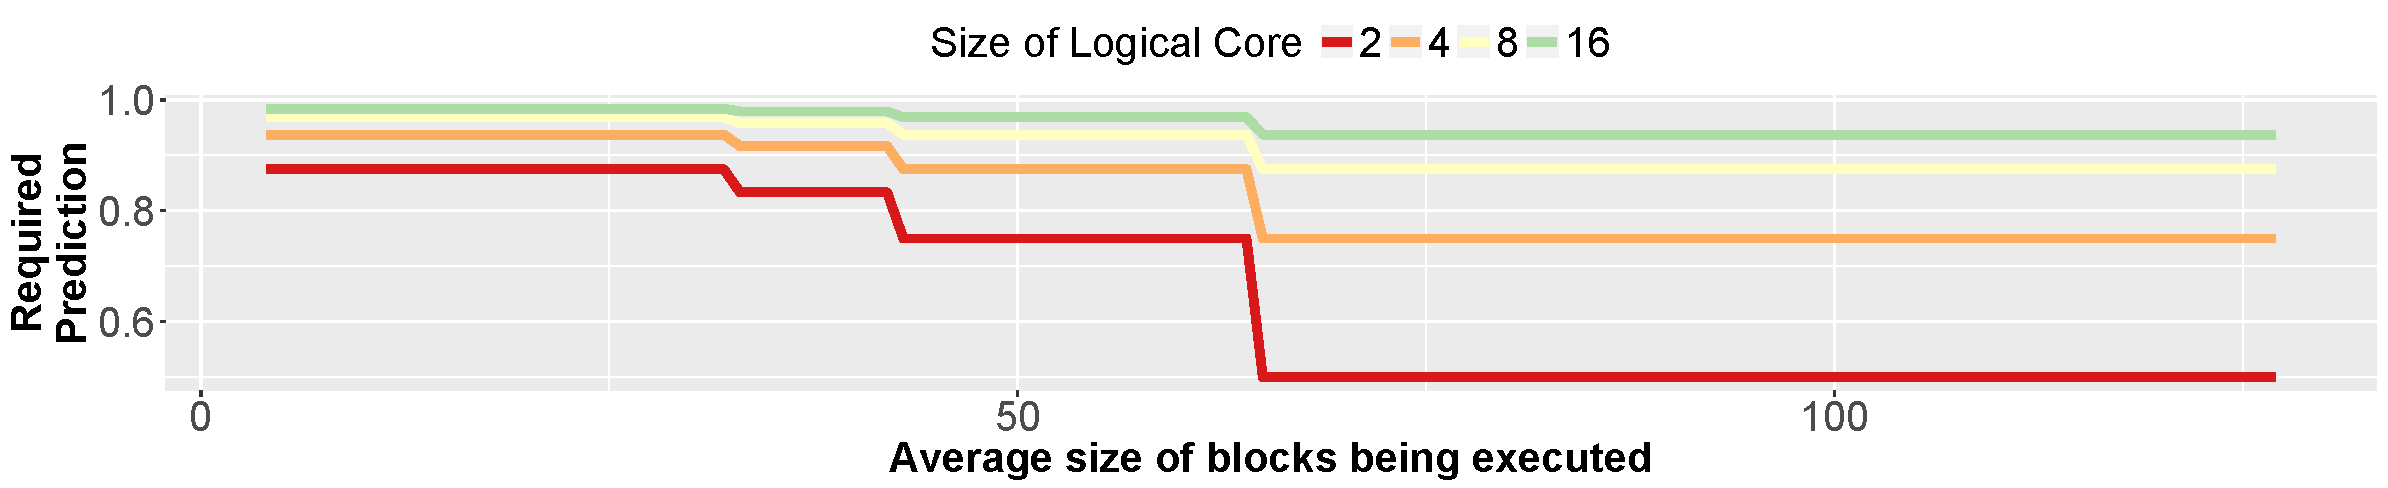
\includegraphics[width=\textwidth]{cases-paper/graphics/limit_study/prediction_req.pdf}
    \caption{Required prediction accuracy for a logical core size to be efficient given an average block size.}
    \label{fig:req_pred}
\end{figure}
\subsection{Synchronization Cost}

For a program to execute correctly, the cores in a logical core (LC) must communicate when they have finished executing a block. 
This ensures that the cores fetch blocks from the correct control paths and update memory and registers consistently.
A core may have to wait for other cores to commit before fetching a new block. 
The worst-case estimate of this stall is defined as the \textbf{Synchronization Cost}.

Blocks commit in a sequential fashion with the non-speculative block committing first and the most recent speculative block committing last.
If a core's instruction window is full then it must commit a block before it fetches a new one.
The Synchronization Cost, in cycles, is defined in equation~\ref{form:synccost} and is measured by averaging the overall number of cycles each fused core waits until it can continue to fetch and execute new blocks.
\textit{AvBlocksInFlight} represents the average number of blocks in flight on a single core in the LC.
This is a worst-case estimate as block sizes will fluctuate during the execution of a program.

\begin{equation}\label{form:synccost}
SyncCost_i = \frac{\sum_{n=0}^{i-1}\left(AvBlocksInFlight \right) \times n }{i}
\end{equation}


\begin{figure}[h]
    \centering
    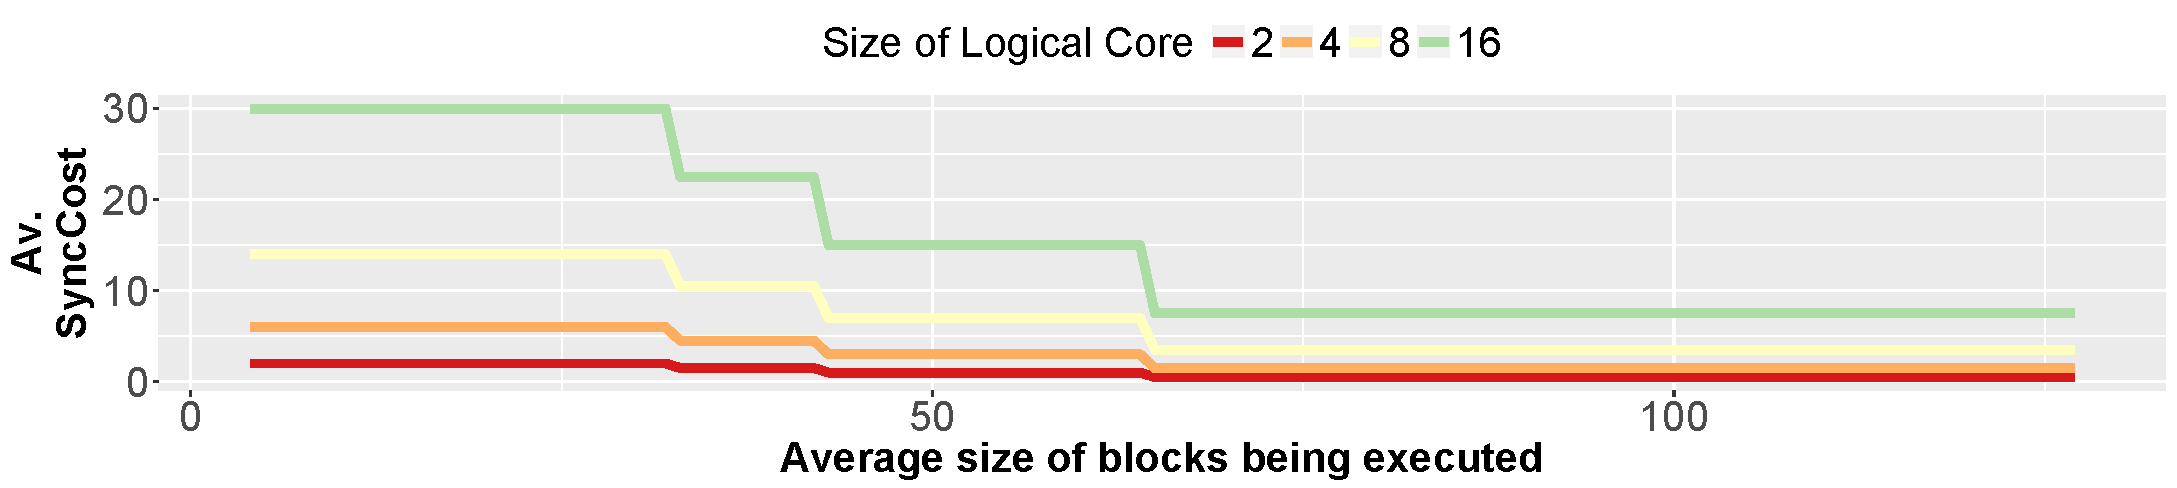
\includegraphics[width=\textwidth]{cases-paper/graphics/limit_study/sync_cost.pdf}

    \caption{Synchronization Cost in cycles for a given number of cores in a composition and an average block size.} %Each core has 4 lanes and each lane can fetch a block of up to 32 instructions. Lower is better.}
    \label{fig:sync_cost}
	\vspace{1em}
\end{figure}

Figure~\ref{fig:sync_cost} shows how many cycles the Synchronization Cost will be for a given LC and average block size.
The larger the block size the lower the Synchronization Cost is since cores fetch fewer blocks and wait less for other fused cores to finish committing.
Large LCs executing small blocks have a high Synchronization Cost. 
This indicates that large LCs should be avoided when dealing with smaller blocks as the Synchronization Cost outweighs the code execution.

\subsection{Summary}

This section estimates the worst-case IPC for a logical processor using Average Block Size, Average Branch Prediction, and Synchonization Cost.
Figure~\ref{fig:lm_summ} presented a worst-case estimate of IPC performance assuming each core can sustain an IPC of 2.
From what was previously explained, Figure~\ref{fig:lm_summ} shows us that to obtain optimal performance requires a high branch prediction accuracy and large blocks.
It shows that larger logical processors can easily under-perform; for example it can be seen that 16 fused cores often have IPCs under 15, meaning that each core has an IPC under~1.

\begin{figure}[t]
    \centering
    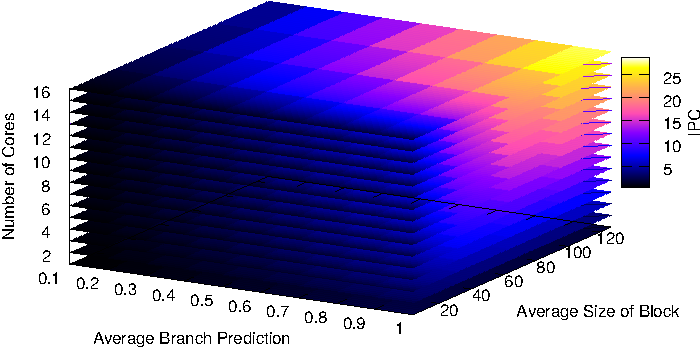
\includegraphics[width=0.8\textwidth]{cases-paper/graphics/limit_study/summary.pdf}
    \caption{IPC estimate given a logical processor size, average branch prediction and average block size for a dual-issue core. A higher IPC means better performance.}
    \label{fig:lm_summ}
\vspace{5mm}
\end{figure}


\section{Methodology}\label{sec:setup}
This section now presents the experimental setup used for the remaining parts of the chapter where a thorough evaluation of core composition is conducted with the cycle-level simulator described in Chapter~\ref{chp:setup} Section~\ref{chp:setup:conf}.

\subsection{Benchmarks}

For this chapter the performance of the Dynamic Multicore Processor (DMP) is studied on a set of Vision Benchmarks designed for hardware and compiler research~\cite{sdvbs} described in Chapter~\ref{chp:setup} Section~\ref{chp:setup:conf}.
The San Diego Vision Benchmark suite (SD-VBS) is composed of nine single-threaded C benchmarks ranging from image analysis to motion tracking.

\begin{table}[t]
  \small
  \centering
 \begin{tabular} {| l | l | l | l | l | l | }
 \hline
   & \cellcolor[gray]{0.7}Disparity & \cellcolor[gray]{0.7} Localization& \cellcolor[gray]{0.7} MSER& \cellcolor[gray]{0.7} Multi\_NCut& \cellcolor[gray]{0.7} Sift\\ \hline
Input&	VGA  & VGA & CIF  & SIM\_FAST& CIF\\ \hline
Cycle Count	&682M  & 526M & 175M  & 180M& 1445M\\ \hline
	
	 & \cellcolor[gray]{0.7} Stitch & \cellcolor[gray]{0.7} SVM & \cellcolor[gray]{0.7} Text. Synth & \cellcolor[gray]{0.7} Tracking&\\ \hline
	  Input & CIF& CIF& FULLHD& VGA &\\ \hline
Cycle count &	  	  571M& 577M& 516M& 374M &\\ \hline

	\end{tabular}
  \caption{Datasets used for each of the benchmarks and the execution time (in cycles) for each of the benchmarks.}\label{tab:sd-data}
  \vspace{2em}
\end{table}


\paragraph*{Input Size}
%Maybe find a way of explaining how long it takes
The SD-VBS benchmark suite comes with a different set of input sizes.
Due to executing these benchmarks on a cycle accurate simulator, executing on large datasets can take a large amount of time.
A single experiment can take up to 6 hours on a single machine (Intel i5 3570k 3GHz, 16 GB of DDR3 RAM), and the average Million instructions per second (MIPS) of the simulator is of 0.1 when only simulating a single core.
In the paper describing each of the applications in the SD-VBS suite~\cite{sdvbs}, Venkata et al. show that increasing the size of the input does not drastically change the phases of each benchmark.
Table~\ref{tab:sd-data} shows the datasets used for the benchmarks in this chapter.
For this chapter, the aim is to have a dataset that leads to executing at least 100 million cycles as this ensures that the caches and branch predictor are warmed up~\cite{dubach13dynamic}.
The execution time for each of the programs, using a single core, can be found in Table~\ref{tab:sd-data}.
%Multi_NCut would take 10x time longer on anything else


%\subsection{Architecture and Simulator}

%A cycle-level simulator of an EDGE-based Dynamic Multicore Processor~\cite{e2} is used, whose core pipeline is verified against an RTL implementation within 5\%. 
%This validation is done by running workloads on RTL and comparing the traces cycle-by-cycle with the software simulator.
%The architecture and core fusion mechanics are similar to the work described in~\cite{kim2007tflex,putnam2010e2}.
%he simulator is configured to model a 16 core multiprocessor, with 32 KB private L1 caches, and allow each core to fetch up to 4 blocks of instructions, 
%and issue up to 2 instructions per block for a maximum of 64 blocks in flight.


%\subsection{Compiler}
%Each benchmark is compiled with the Microsoft C++ compiler for EDGE~\cite{e2}, with -O2 optimisations and using instruction predication for hyperblock formation~\cite{smith2006edge}.

\subsection{Measuring Performance and Power}

The objective of the chapter is to explore how adapting the DMP to the phases of an application can affect performance.
To evaluate dynamic adaptation, it is compared to different static ahead of time configurations.

Five simulations per benchmark are ran, one for each core composition size: 1, 2, 4, 8 and 16.
For each the IPC is recorded at an interval of 640 committed blocks.
640 committed blocks is chosen as it allows each core in a core composition to execute enough blocks before taking the measurement.
This is due to the fact that the highest core composition of 16 cores can execute up to 64 blocks at a time, thus recording performance after 640 blocks allows each core to have executed at least 10 blocks.
Using committed blocks allows us to easily compare each simulation as the total number of committed blocks does not change even if the core compositions are different.

The EDGE architecture is fundamentally different from the traditional CISC/RISC paradigm and thus, McPAT~\cite{mcpat} cannot be used to model power consumption as it differs from traditional CISC/RISC cores modeled in McPAT.
Instead a coarse grained power model is used where power gating is applied; when a core is not currently being used, it is assumed to be turned off and therefore does not consume energy.

\section{Code Optimisations}\label{sec:opt}
\begin{figure}[t]
\begin{minipage}[t]{0.48\textwidth}
\lstset{language=C,numbersep=4pt,basicstyle=\small}
\begin{lstlisting}
for(int i = 0; i < 1000; i++)
  for(int j = 0; j < 1000; j++)
     for(int k = 0;k < 5; k++)
         a[i][j] = a[i][j] * b[k][j];
\end{lstlisting}
\vspace*{-5mm}
\caption{Example of an inner-most loop which should be completely unrolled.}
\label{lst:small}
\end{minipage}
\hfill
\begin{minipage}[t]{0.48\textwidth}
\lstset{language=C,numbersep=4pt,basicstyle=\small}
\begin{lstlisting}
for(int i = 0; i < 1000; i++)
  for(int j = 0; j < 1000; j++)
      a[i][j] = a[i][j-1] 
                       * b[i][j];
\end{lstlisting}
\vspace*{-5mm}
\caption{Example of a data dependency which can be removed by interchanging the loops.}
\label{lst:dep}
\end{minipage}
\vspace{9mm}
\end{figure}

This section describes optimizations focused on reducing control flow and expanding block sizes which is necessary for high performance as seen in section~\ref{sec:lim_study}.

\subsection{Loop Unrolling}
Loop unrolling is a common optimization used to reduce the overhead of the loop header and to better expose Instruction Level Parallelism (ILP).
When dealing with tightly-knit loops, logical cores may perform poorly due to the fact that they execute many small blocks, thus increasing the Synchronization Cost.
Unrolling loops will both reduce the number of blocks required to execute the loop and increase the size of the blocks, thus reducing the Synchronization Cost and increasing ILP.
For example, the innermost loop in Figure~\ref{lst:small} should be completely unrolled and its outer loop unrolled partially to increase the block size.
There are certain factors which can limit the usefulness of loop unrolling which we examine later on.
In the architecture we evaluate, we may not have more than 32 load or store instructions per block.
Therefore, if we unroll memory intensive loops, we must ensure we do not go above this threshold.
Going above this threshold leads to creating a new block which will put a strain on the branch predictor.
Another issue is that unrolling loops with conditional statements may not help improve the size of the block as the conditional branches might still segment the new blocks.
So we should avoid unrolling such loops.



\subsection{Loop Interchange}
When dealing with nested loops there is one reason we have determined for interchanging the loops.
The case arises when interchanging the loop removes dependencies in the inner-most loop.
The dependency in Figure~\ref{lst:dep} can be removed by interchanging the loops. 
This allows us to unroll the inner loop efficiently, but also remove any kind of dependency between blocks.
Since two blocks from the same loop may execute on different cores, we want to reduce any kind of data dependency, minimizing core communication.

\begin{figure}[t]
     \centering
     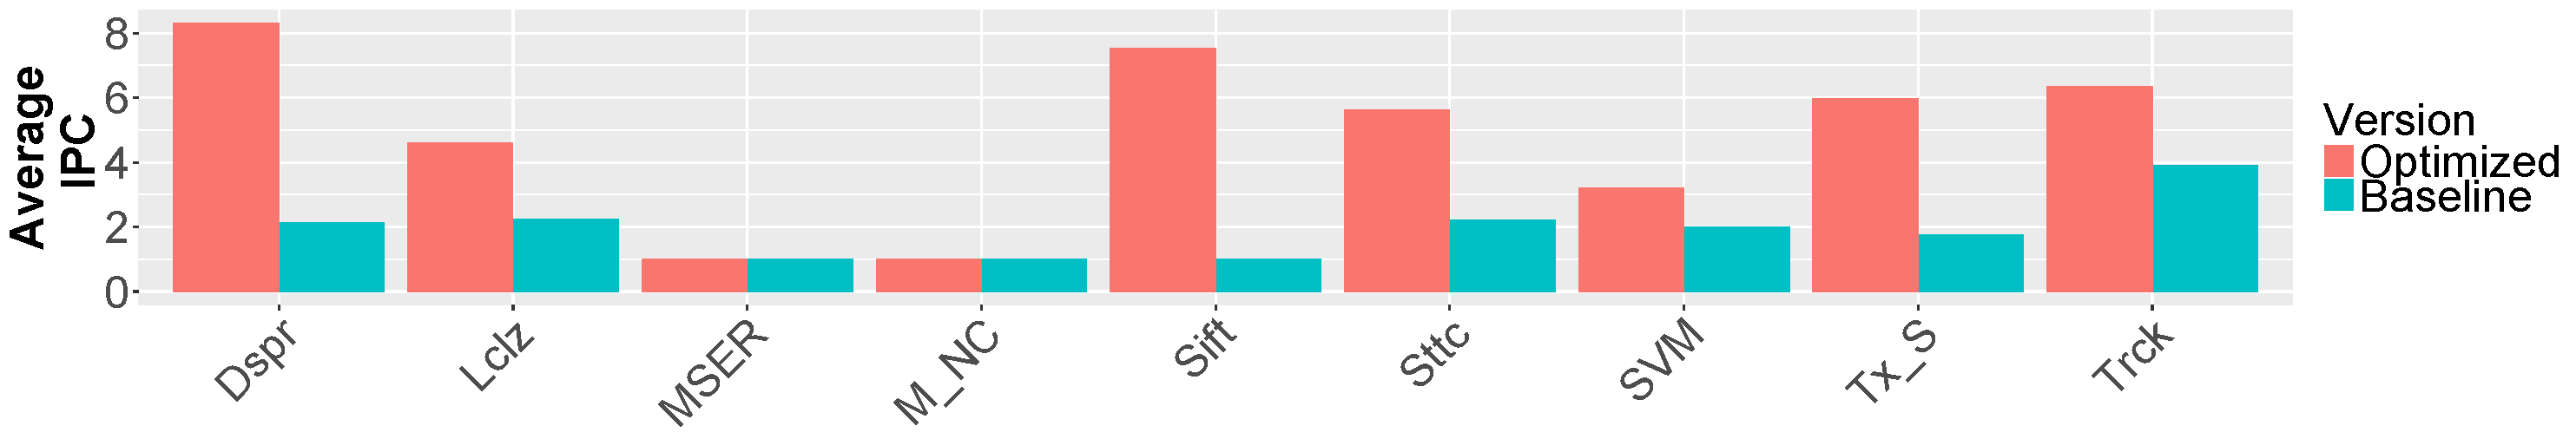
\includegraphics[width=\textwidth]{graphics/Exploration/ipc_comp.pdf}
\vspace*{-8mm}
     \caption{Average IPC using the optimal sized logical-core, with and without optimizations. Higher is better.}
     \label{fig:ipccom}
     \vspace{0.5em}
\vspace{5mm}
    \centering
    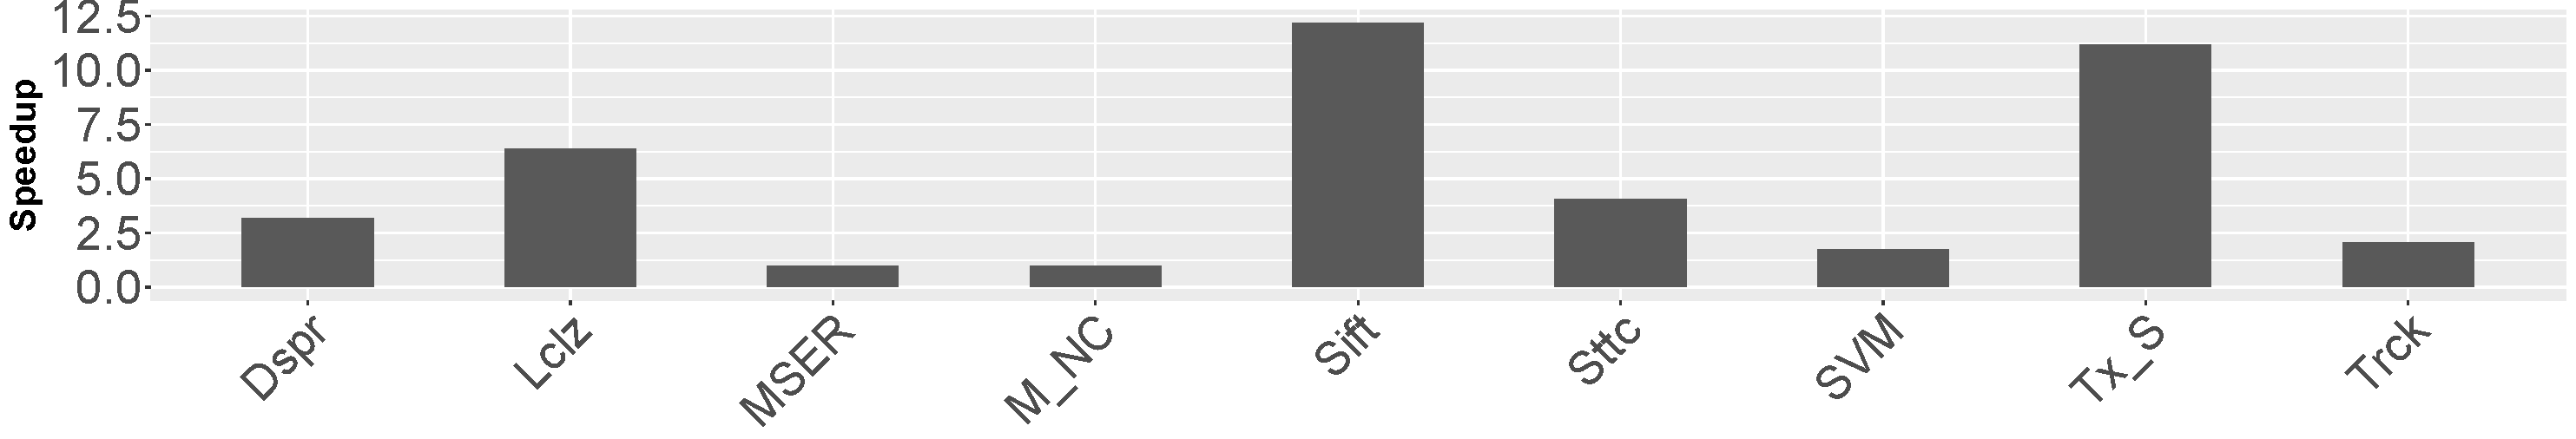
\includegraphics[width=\textwidth]{graphics/Exploration/comp_speed.pdf}
\vspace*{-8mm}
    \caption{Speedup from using code-optimizations over baseline source code using the same optimal sized logical-core.}
    \label{fig:speedcomp}
\vspace{5mm}
\end{figure}

\subsection{Predication and Hyperblock Formation}
EDGE compilers must split blocks whenever control-flow is present~\cite{smith2006edge}.
If a loop contains a conditional statement, the loop body has to be split in two unless if-conversion is applied.
Hyperblock formation aims to reduce branching and increase block size by combining two or more blocks into a single predicated block~\cite{smith2006edge}.
Hyperblocks reduce both synchronization cost and branch prediction requirements as discussed previously.
This is especially important in control-flow intensive loops where unrolling increases the number of conditional statements.

\vspace{5mm}
\subsection{Results}

While the optimizations described above and their tuning would be easy to implement in a compiler, we did not have access to the compiler's source code.
We therefore modified the source code of our benchmarks by manually interchanging or unrolling loops.
In the case of predication and hyperblock formation, we converted simple if-then-else statements into ternary operators whenever possible.
We also tried to reorder statements within the body of a loop to avoid having control flow in the middle of the body.
We then verified that our source code modification had the intended effect by dissembling the binary produced by the compiler.
We modified between 0 and 12 loops depending on the benchmark.

We compare the best static core fusion using the optimized code with the unmodified code, both version compiled with \texttt{-O2}.
Figure~\ref{fig:ipccom} shows the resulting IPC for the baseline case and the optimized benchmarks when run on a core with the optimal number of fused core to maximize performance.
The IPC of the baseline is very low for the majority of the benchmarks which might give the impression that core fusion is rather inefficient.
However, after applying the simple optimizations described above, the average IPC is significantly increased in many cases.

Since optimizations change the total number of instructions, we also show the actual speedup obtained using cycle count in Figure~\ref{fig:speedcomp}.
As we can see, benchmarks \bm{MSER} and \bm{Multi-NCut} do not perform any differently.
This is due to the fact that none of these optimizations can be successfully applied on these benchmarks.
For the other benchmarks we see significant improvements of up to 12$\times$ for \bm{Sift} when the optimizations are applied.

\subsection{Summary}

Overall, this section shows that classical loop transformations can have a large impact on the performance of fused cores.
Without these optimizations, it would be more difficult to motivate the use of core fusion even at a static-level as the IPC does not deviate enough from a single core.


\section{Benchmark Exploration}\label{sec:expl}

\begin{figure}[t]
    \centering
    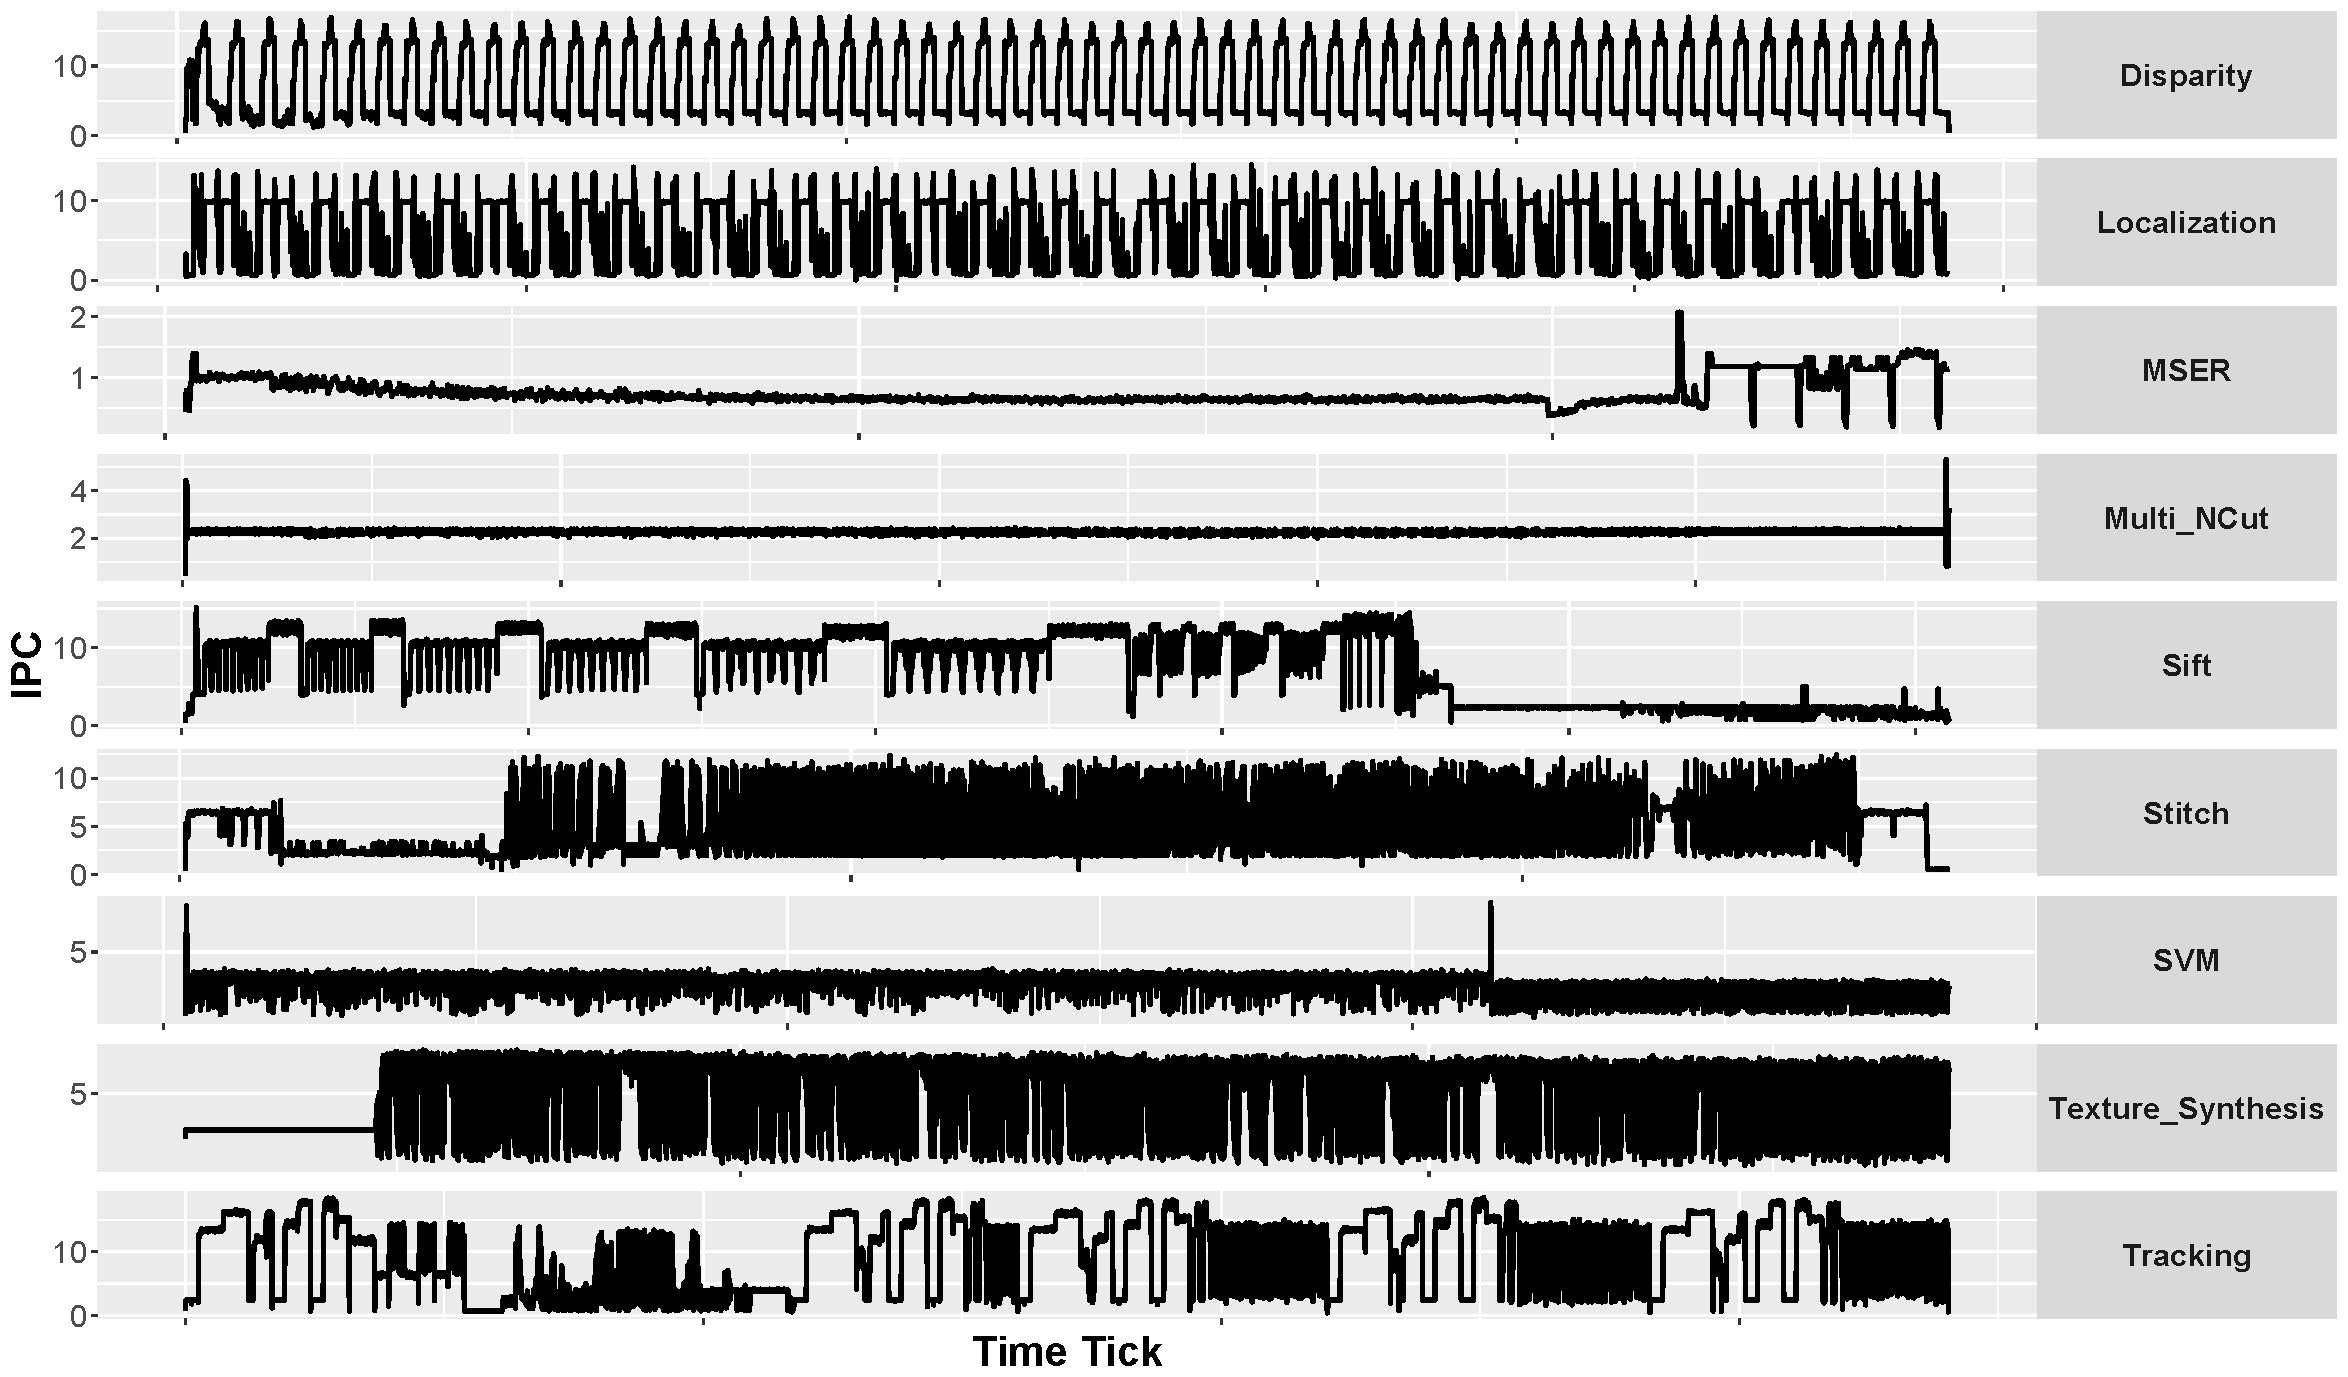
\includegraphics[width=1\textwidth]{cases-paper/graphics/Exploration/ipcs_16_2.pdf}
    \caption{IPC as a function of time for each benchmark when run on 16 fused cores.}
    \label{fig:sxt}
	\vspace{1em}
\end{figure}

This section explores how core composition affects the performance of the SD-VBS benchmarks.
First a phase analysis is performed, followed by a study of the IPC variation for static core fusion.
Then the use of dynamic core composition is motivated by using the gathered information.

\begin{figure}[t]
    \centering
    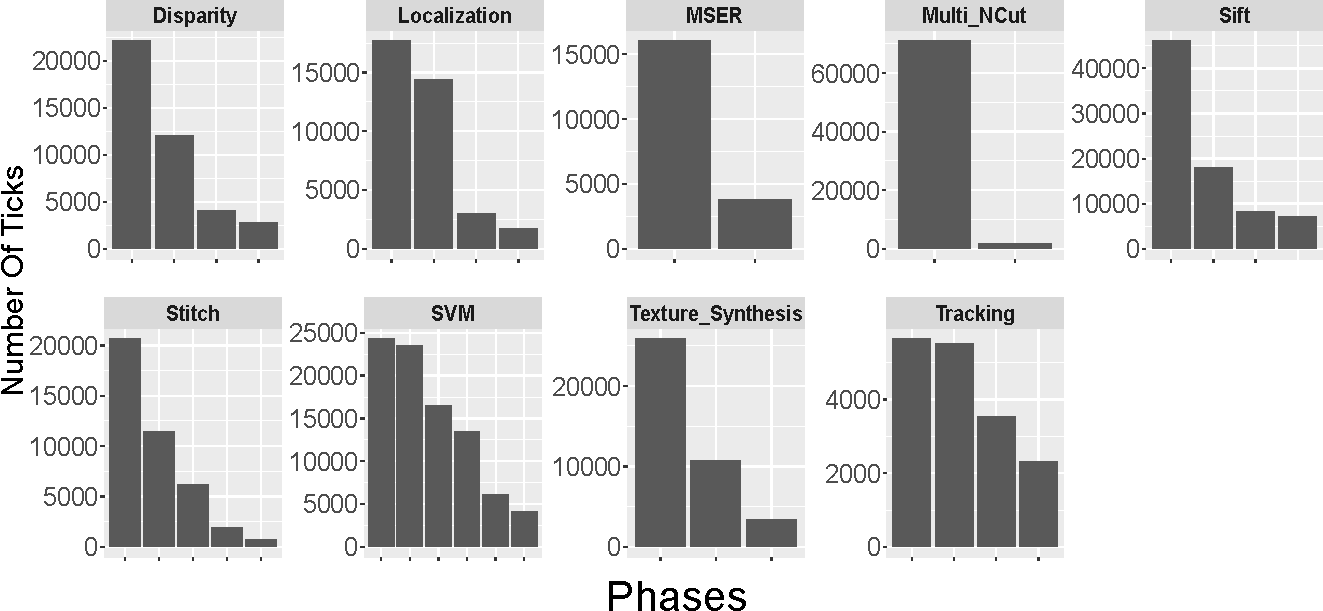
\includegraphics[width=1\textwidth]{cases-paper/graphics/Exploration/clusters3.pdf}
    \caption{Number of phases determined for each benchmark using kMeans clustering and their distribution.}
    \label{fig:clust}
		\vspace{1em}
\end{figure}


\subsection{Phase Detection}
Figure~\ref{fig:sxt} presents the IPC performance through time for all the benchmarks when using a logical core (LC) composed of 16 cores.
The IPC is calculated for each time tick, which is set at interval of 640 blocks committed.
%make this way clearer
The interval of 640 blocks was chosen as the largest core composition of size 16 can potentially commit up to 64 blocks at a time.
Thus measuring performance every 640 blocks allows to fully capture the performance of large compositions without sacrificing loss of information.
Displaying the performance of the LC of size 16 gives a performance ceiling for all the benchmarks as it is the maximum number of cores which can be fused at any point.
As seen in Figure~\ref{fig:sxt} the IPC varies a lot for some of the benchmarks such as \bm{Disparity} or \bm{Localization} where dynamic fusion is expected to be especially good.
For other, such as \bm{Multi\_NCut}, the execution is dominated by a single long phase with constant IPC, which will clearly show no benefit from using dynamic fusion.

To better understand how dynamic core fusion improves performance, either by improving speedup or reducing energy, this section begins with a study of how each benchmark features different phases during their execution.
For every benchmark the IPC results of 16,8,4,2,1 fused cores are regrouped and kMeans clustering is applied to determine phases.
Intervals that exhibit similar IPC values when run on different core counts are classified in the same cluster.
In order to find the correct number of clusters the Sum of Square Errors (SSE) is plotted for a given cluster size from 1 to 15 and determine the optimal cluster to be in the elbow in the plot~\cite{everitCluster2001}.
Applying a kMeans clustering to the IPCs of each application to determine phases is preferred to determining phases of an application by reading the source code phases.
For example, the benchmark \bm{MSER}'s source code has 7 distinct steps, yet the kMeans clustering shows that most of these steps result in the same performance, which can be visualised in Figure~\ref{fig:sxt}.
This kMeans clustering process is only done for the purpose of exploring this set of benchmarks.

Figure~\ref{fig:clust} shows the number of clusters for each benchmark and the frequency of each cluster.
The frequency of a cluster is counted by how many ticks in the program are part of that specific phase.
The data can be corroborated with the information found in Figure~\ref{fig:sxt}.
For example, benchmarks \bm{MSER} and \bm{Multi\_NCut} feature two phases, with one of those phases comprising over 80\% of the total execution.
This means that it will be impossible to obtain any kind of performance improvements through dynamic reconfiguration due to the fact that there is little opportunity to switch the size of the LC.
For all the other benchmarks, they each have at least two dominant phases.
Since each phase is a cluster of similar IPC values, having two or more clusters will result in a higher chance of benefiting from dynamic core fusion.

\begin{figure}[t]
    \centering
    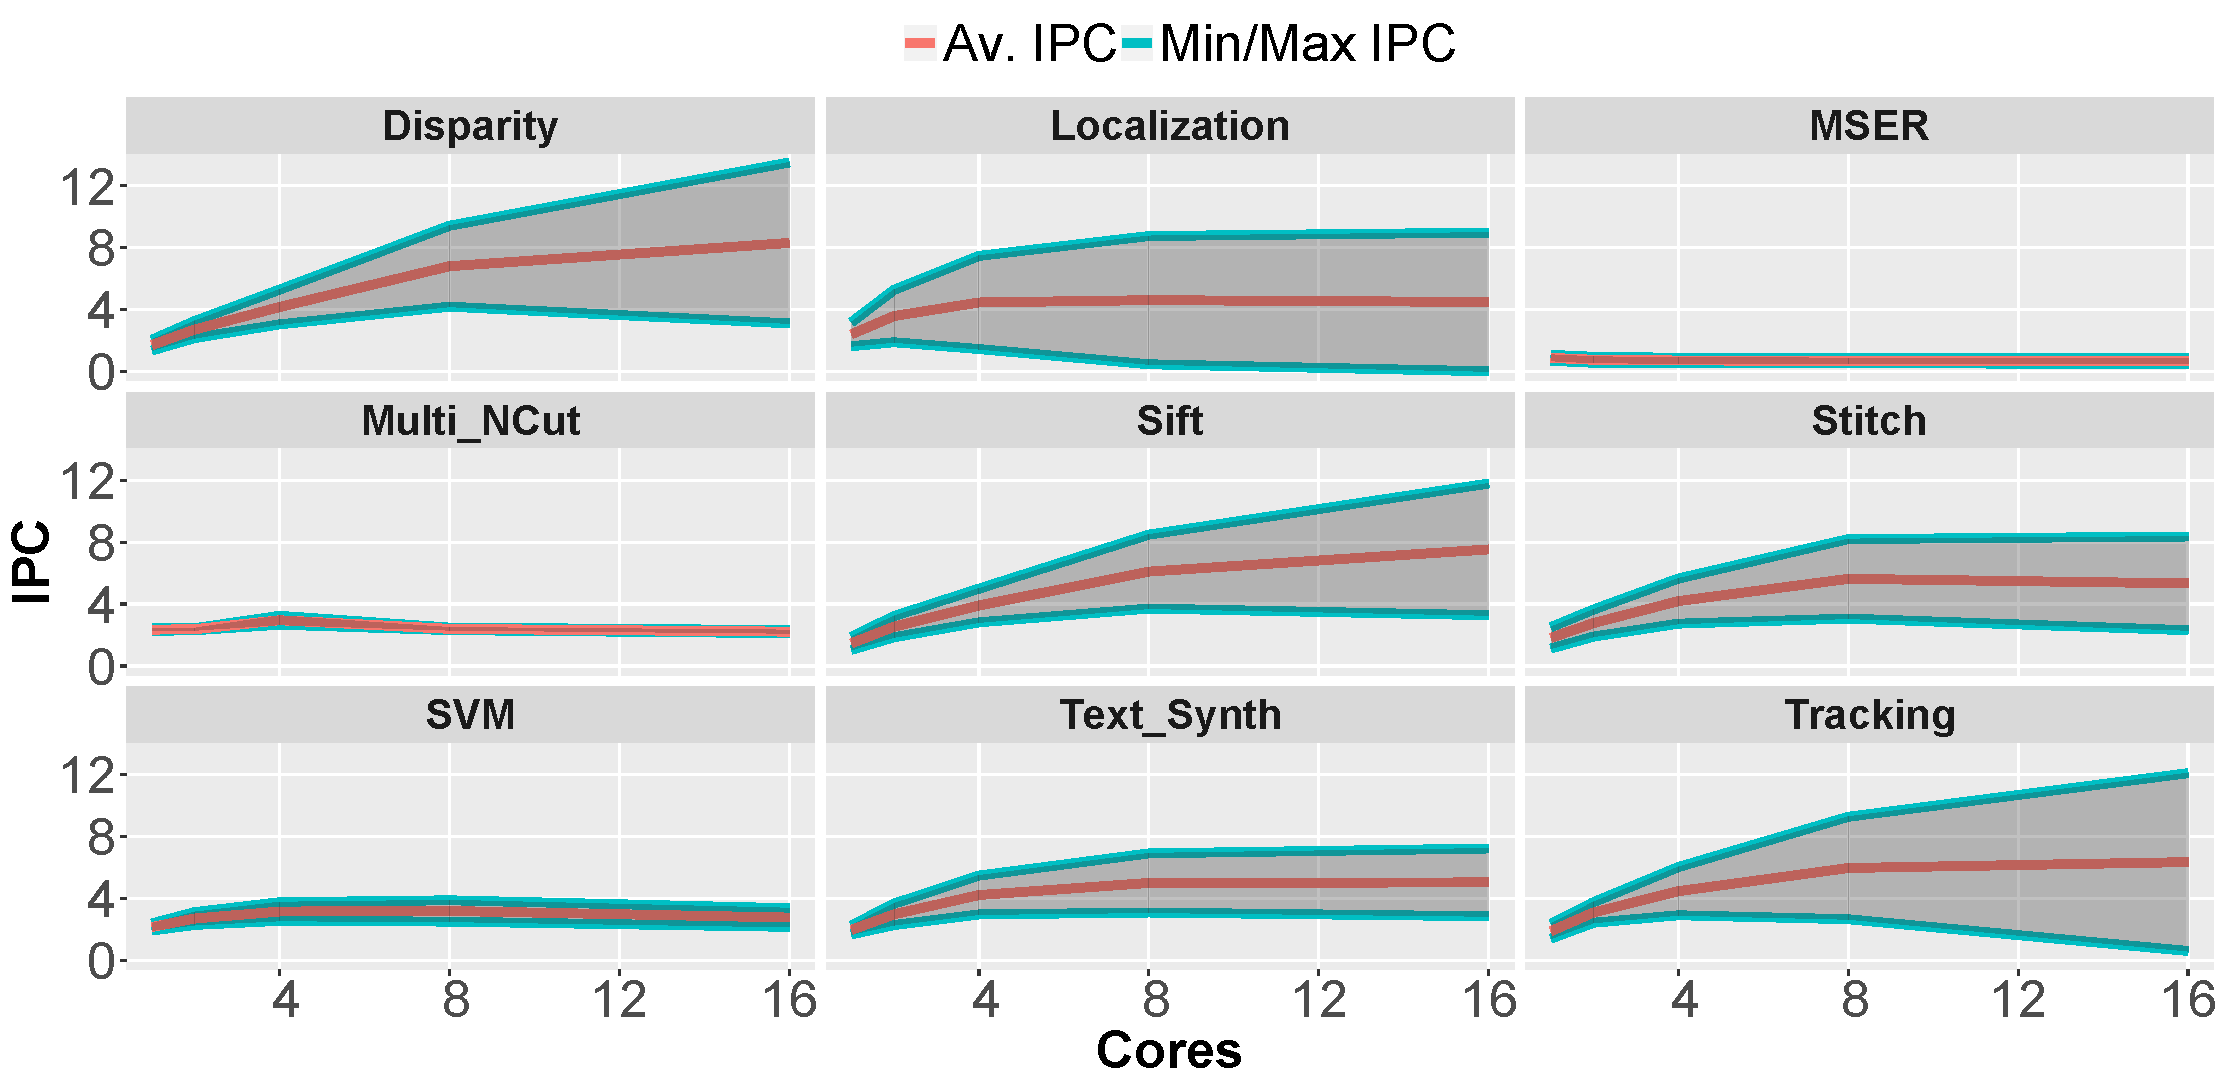
\includegraphics[width=1\textwidth]{cases-paper/graphics/Exploration/stddev2.pdf}
    \caption{Comparing average, smallest and greatest IPC for each SD-VBS benchmark using logical-core size of 16.}
    \label{fig:stddev}
		\vspace{5mm}
\end{figure}

\begin{figure}[t]
    \centering
    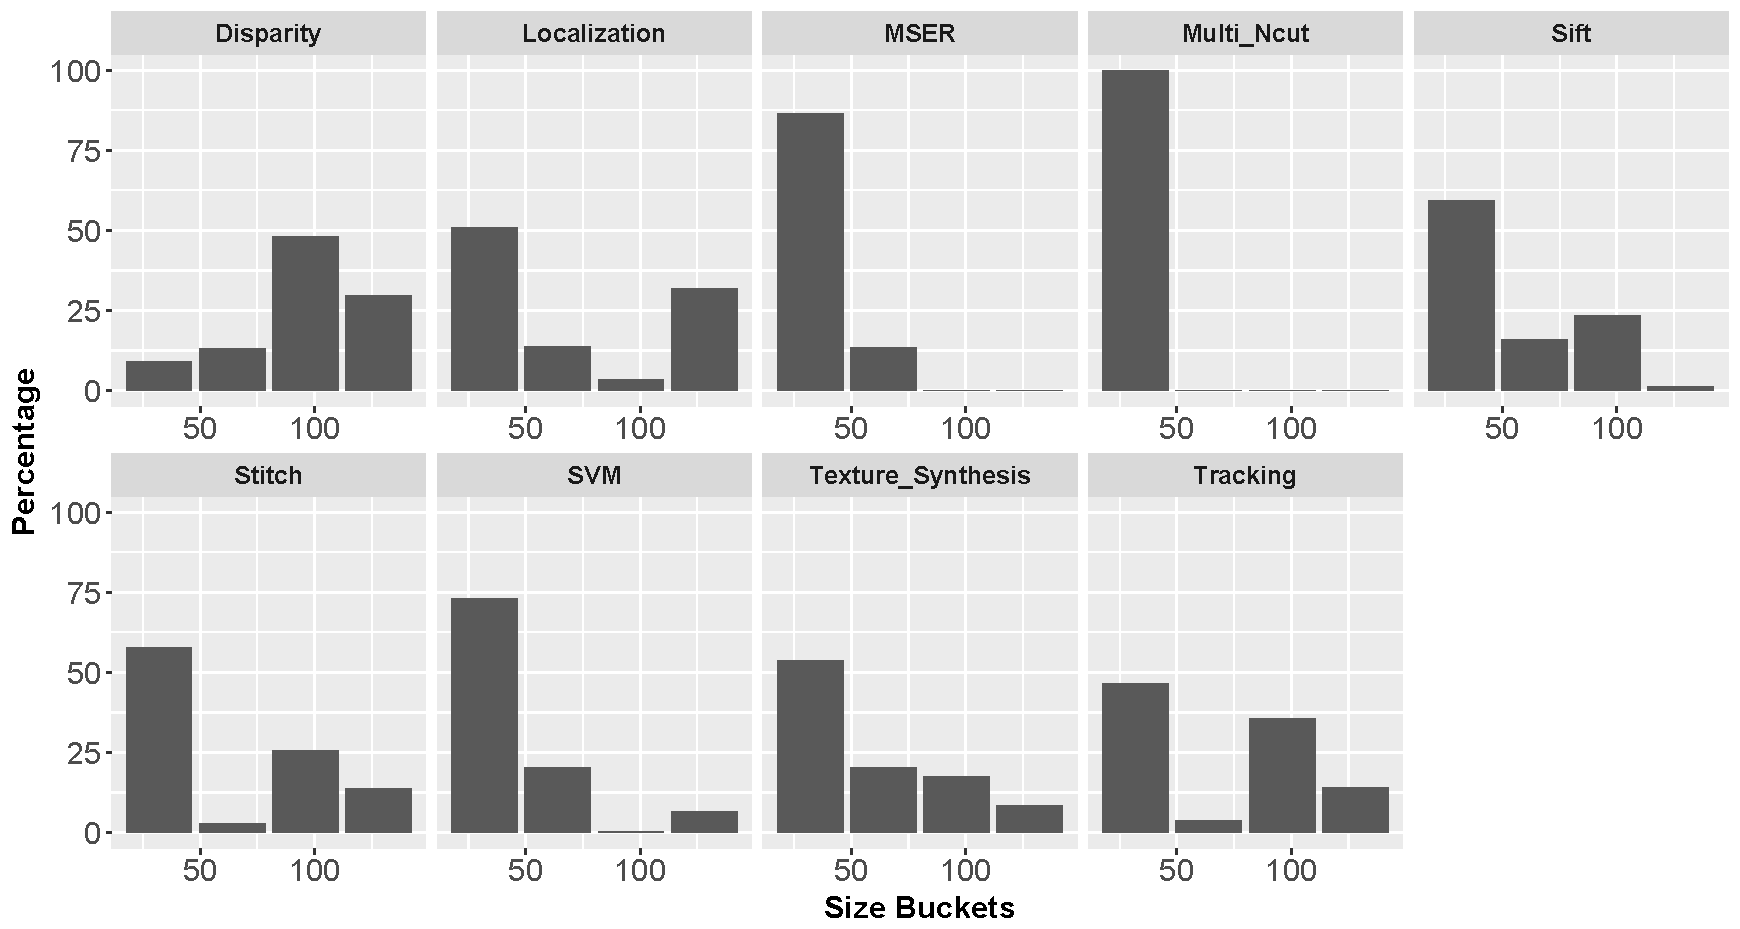
\includegraphics[width=1\textwidth]{cases-paper/graphics/Exploration/SizeBuckets.pdf}
    \caption{Distribution of block sizes for each benchmark. The sizes are clustered in buckets equivalent to number of lanes occupied.}
    \label{fig:block_sizes}
	\vspace{5mm}
\end{figure}

\subsection{Static Core Fusion Exploration}

Figure~\ref{fig:stddev} shows how the average Instructions Per Cycle (IPC) changes as the size of a LC is increased, going in powers of 2 from 1 to 16 fused cores.
It can be seen that, for most benchmarks, fusing more cores provides an increase in IPC performance.
Benchmarks \bm{Disparity}, \bm{Localization}, \bm{Sift}, \bm{Stitch}, \bm{Texture Synthesis} and \bm{Tracking} all at least observe a speedup of 2x when using core fusion.

However increasing the size of a LC is not always beneficial as can be seen in benchmarks \bm{Localization}, \bm{MSER}, \bm{Multi\_NCut}, \bm{Stich}, and \bm{SVM}.
For benchmarks \bm{Localization} and \bm{Stitch} the performance increases when fusing up to 8 cores, where-as \bm{MSER} and \bm{Multi\_NCut} never benefit from core fusion.
These benchmarks may not see a reduction in performance on 16 cores due to the increase in network traffic, which will make the highest LC size slower than 8 cores.
Referring back to Figures~\ref{fig:sxt} and~\ref{fig:clust}, \bm{MSER} and \bm{Multi\_NCut} feature one dominating long phase, both performing poorly.

Figure~\ref{fig:stddev} also shows the standard deviation of the IPC for each given LC size represented by the grayed out areas.
For example, running the \bm{Disparity} benchmark on a LC of 16 cores, it can be observed that an average IPC of 8.3 with a standard deviation of 5.2.
The standard deviation for 16 cores shows that the performance can drop down to 2.5.
An IPC of 2.5 when using 16 cores is very inefficient as this represents 0.1 of an instruction per cycle for each core.
Using a LC of size 4 for the \bm{Disparity} benchmark an average of 4.1 with a standard deviation of 1.2 is achieved.
Thus, if the logical-core could change size, there is a possibility that this could reduce the overall energy consumption of the system by switching from 16 to 4.

Figure~\ref{fig:block_sizes} shows the distribution of block-sizes for each of the benchmarks.
As two blocks cannot occupy the same lane, the block sizes are clustered into groups which represent how ever many number of lanes will be occupied (one lane may execute a block of up to 32 instructions).
Figure~\ref{fig:block_sizes} helps explain why benchmarks \bm{MSER} and \bm{Multi\_NCut} do not perform any better with core-fusion.
For both cases, not only do they have a single detected phase, but both are predominantly formed of blocks that will occupy a single lane.
In fact, the most frequent block in \bm{MSER}, comprising 21\% the total executed blocks are comprised of only 8 instructions, whilst 31\% of \bm{Multi\_NCut}'s blocks are of 28 instructions.
Having such small blocks will always increase both the \textit{SynchronizationCost} and the branch-prediction requirements.
For \bm{MSER}, the fact that an important percentage of blocks are only 8 instructions long signifies that the overhead of fetching enough blocks for a large core-composition and the synchronization cost for committing them outweighs executing the blocks on a single core.
The reason there is no degredation of performance is due to the fact that when fusing a high amount of cores, if the overhead of fetching the blocks outweighs the time required to execute them, cores will simply not execute blocks.
For example, fusing 16 cores and executing \bm{MSER} may in fact result in a single core being used due to it executing blocks faster than it being able to dispatch the blocks to a next core.
Hence, in this case, \bm{MSER} would be wasting a lot of energy trying to use 16 cores in a composition, whilst effectively only executing on a single core. 
This explains the lack of scaling for these two benchmarks.
The source-code of \bm{MSER} and \bm{Multi\_NCut} is explored later on, to demonstrate how such small blocks are generated and why it cannot be improved.

Overall, most benchmarks that benefit from large logical-cores will also be met with important standard deviations of IPC performance.
The high standard deviation is evidence of performance phases found in each application which are likely to benefit from dynamic adaptation.

%Need a better name for this
\subsection{Analysis of loops}

\begin{table}[t]
  \small
  \centering
 \begin{tabular} { | l | l | l | l | l | }
 \hline
   \cellcolor[gray]{0.7}Disparity & \cellcolor[gray]{0.7} Localization& \cellcolor[gray]{0.7} MSER& \cellcolor[gray]{0.7} Multi\_NCut& \cellcolor[gray]{0.7} Sift\\ \hline
	98\%  & 95\% & 85\%  & 100\%& 99\%\\ \hline
	 \cellcolor[gray]{0.7} Stitch & \cellcolor[gray]{0.7} SVM & \cellcolor[gray]{0.7} Text. Synth & \cellcolor[gray]{0.7} Tracking&\\ \hline
	  95\%& 93\%& 98\%& 98 \%&\\ \hline
	\end{tabular}
  \caption{Branch prediction accuracy in percentage for each of the benchmarks.}\label{tab:sd-vbsbpred}
  \vspace{1em}
\end{table}

As previously mentioned, both \bm{MSER} and \bm{Multi\_NCut} do not benefit from core-composition during their predominant phases'.
This subsection focuses on understanding why this is the case and explores the code that represent the main phases of both of these applications to underline where the problems arise.
%Other code snipets from other SD-VBS benchmarks are also explored to demonstrate examples of code that perform well on core-compositions.

\paragraph{MSER}
\bm{MSER} has two distinct IPC phases according to Figure~\ref{fig:clust}, in the code the first phase, which is the domminant phase, represents the computation of the extremal regions tree.
As seen in Figure~\ref{fig:block_sizes}, the majority of the blocks in MSER are less than 32 instructions long, meaning that core-compositions will have to load the maximum amount of blocks to fill each core.
The source code of this phase can be found in the Appendix with Listing~\ref{lsting:mser}.
The listing shows how this phase is made out of small tight knit loops.
The while loops found at lines 27-30, 31-33, 36-39, 40-42 and 71-75 never run for more than a few iterations.
This entire section of code is full of control-flow causing the blocks to remain very small.

It's also important to note that Table~\ref{tab:sd-vbsbpred} shows that the average branch-prediction accuracy of \bm{MSER} is of 85\%.
Recalling Figure~\ref{fig:req_pred} and the fact that the average block size of \bm{MSER} is under 32 instructions, this means that no composition can be fully efficiently used.
Some speedup can still be obtained, as cores in a composition do not need to have all the instruction window full to be able to obtain performance improvements.
However these improvements are minor, and come at a high energy cost.

To get performance out of \bm{MSER}, this major phase would have to be re-written to be less control-flow heavily so that larger blocks can be extracted.

\paragraph{Multi-NCut}
\bm{Multi\_NCut} is faced with a similar situation to \bm{MSER}.
Figure~\ref{fig:block_sizes} shows that once again, the majority of the blocks are less than 32 instructions long, in fact, over 50\% of the blocks are of 12 instructions or less.
Table~\ref{tab:sd-vbspred} shows that the branch prediction is always correct, yet, with blocks this small, the synchronization cost of executing the blocks on large compositions outdoes any benefit that can be obtained via core-composition.
Listing~\ref{lsting:multi} shows the source code of the main phase of \bm{Multi\_NCut}, the main loop found at lines 49 to 58.
Once again, this loop cannot be efficiently unrolled as the \textit{find} and \textit{join} functions are comprised of small control heavy while loops.
Even by inlining those function calls, the while loops will cause the blocks to be small, and unrolling the while loops will generate more checks which wont help increase the size of the blocks.
Overall, for \bm{Multi\_NCut} the problem is that the blocks are too small which will cause the overhead of dispatching multiple blocks across a core-composition inefficient.
This is why the benchmark does not perform significantly better with core-composition without a high increase in energy consumption.


Overall, both benchmarks demonstrate that some loops cannot be adapted to benefit from core-composition.
This is especially true of while loops that cannot be converted into more traditional for loops.
Due to the size of these loops, the overhead of dispatching multiple blocks over multiple cores simply outweighs the performance benefits.

\section{Dynamic Core Composition}\label{sec:dynamic}
The previous section covered the behavior of the program under a static number of cores, now the impact of varying the number of composed cores throughout program execution is now studied.
The section first describe how the traces are generated for the dynamic core fusion schemes.
Before the analysis two types of static core fusion are defined:

\begin{itemize}
	\item \textbf{Static Benchmark}: A fixed fused-core which is optimal for a unique benchmark (SB).
\vspace{-1.2em}
	\item \textbf{Static Suite}: A fixed fused-core which represents the average best for the entire suite of benchmarks. This represents the baseline for the chapter (SS).
\end{itemize}

The reason \textbf{Static Suite} is used as a baseline is due to the fact that it represents a configuration choice at design time.
It is the equivalent of hardware designers analysing the requirements of a processor based on the type of applications it will be executing.
This is better than using a single core as a baseline, as a single core will always represent the slowest execution time whilst also consuming the least amount of energy.
\textbf{Static Benchmark} on the other hand represents the ability to compose cores statically ahead of time; which is an extra step of flexibility compared to \textbf{Static Suite}.

The static core-composition scheme \textit{SS} is compared to the results obtained for the dynamic one for the SD-VBS benchmarks.
This is followed by a closer analysis for two dynamic core fusion objectives: one that optimizes speed and another that optimizes for efficiency.

\begin{figure}[t]
    \centering
	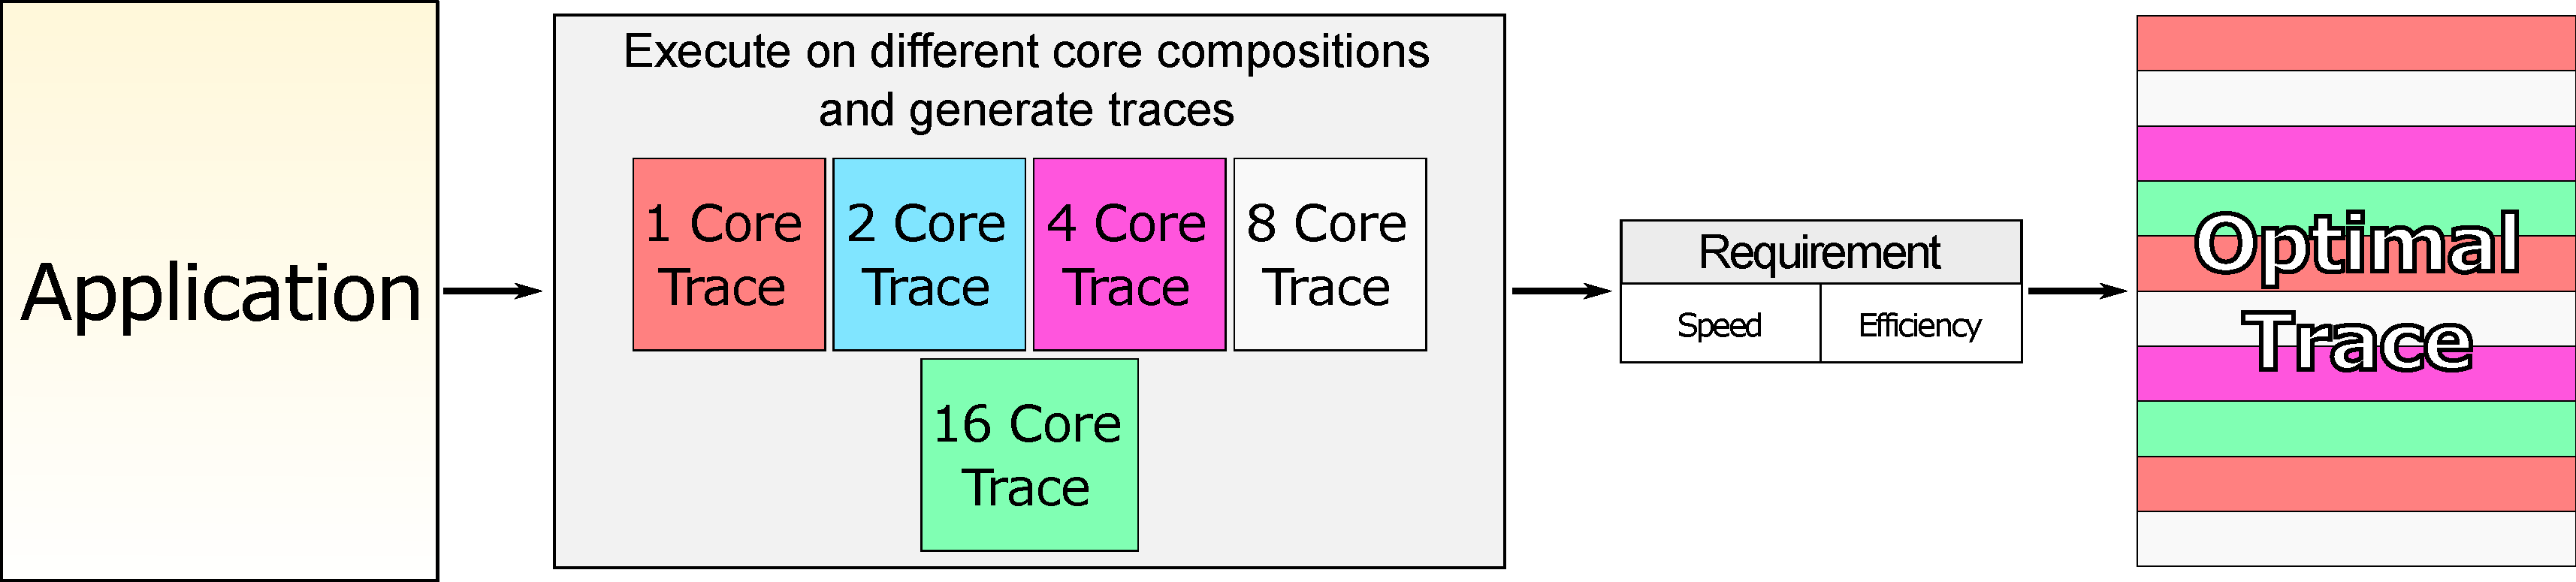
\includegraphics[width=1\textwidth]{cases-paper/graphics/exploration/trace-gathering.pdf}
    \caption{Maximizing speed for all the SD-VBS benchmarks. For Speedup, higher means better, for Energy, lower is better.}
    \label{fig:tracegraph}
	\vspace{1em}
\end{figure}

\subsection{Creating Dynamic Core Composition Traces}

Dynamic core composition enables the ability to change the number of cores for each time tick (an interval of 640 committed blocks) during the execution of a program.
In order to explore the different performance and energy trade-offs that are possible to achieve with this technique, traces of execution for the application are collected.
Figure~\ref{fig:tracegraph} is a visual overview of how dynamic traces are collected.
First application is run on 1,2,4,8 and 16 fused cores and the performance is recorded for each time tick of 640 committed blocks.
Using these 5 traces, any dynamic execution can be constructed to generate dynamic traces.
For this chapter, the dynamic trace will be generated base on one of two requirements; that it maximise speed or maximise efficiency.

To simplify the exploration process, time ticks that are attributed to the same phase are always given the same number of cores.
This is done to reduce the search space as on average there are 48494 ticks which results in an average of $5^{48,494}$ different possible executions.
Since the maximum number of clusters found is 6 (for SVM), a maximum of $5^{6} = 15625$ different dynamic execution traces can be built.
This is why creating dynamic core-composition out of traces is prefered to running all potential dynamic configurations via the simulator.
All applications run for a couple hundred million cycles, which often takes a couple of hours to execute.
As the amount of dynamic reconfigurations is high for some benchmarks, using traces to simulate dynamic reconfiguration is a very large time-save.
When the size of the logical core (LC) is switched, the performance of that LC from its respective trace file is used and an extra 100 cycle penalty is added for switching the size of a LC.
With all these different dynamic core fusion traces, the optimal schemes for maximizing speed or maximizing efficiency can be found.

\begin{figure}[t]
     \centering	
	 \vspace{-1em}
     \subfloat[][Disparity]{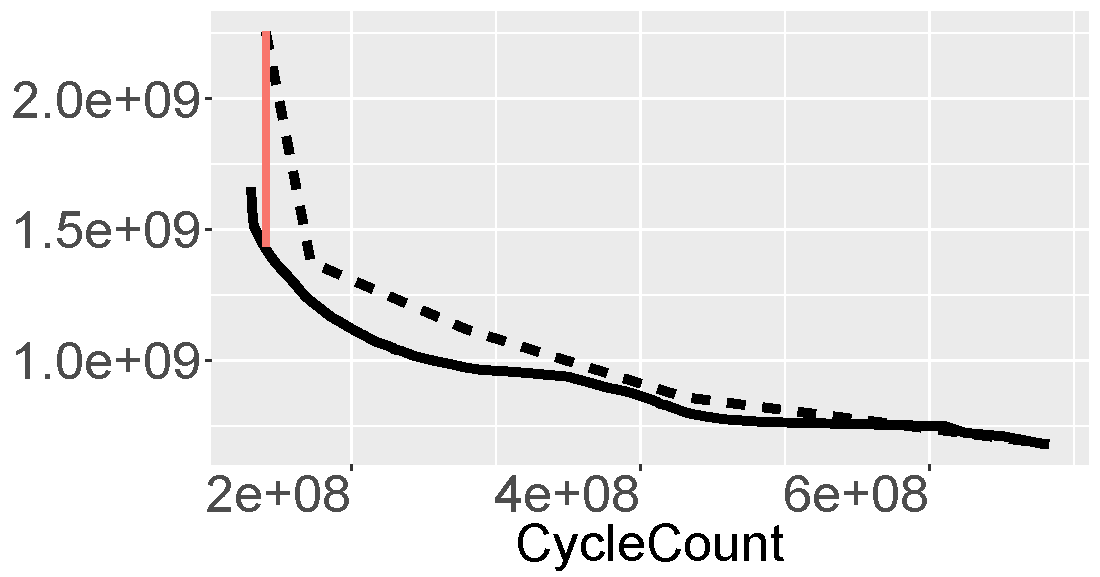
\includegraphics[width=0.3\textwidth]{cases-paper/graphics/Pareto/DispN3.pdf}\vspace*{-4mm}\label{subfig:disp}}
     \subfloat[][Localization]{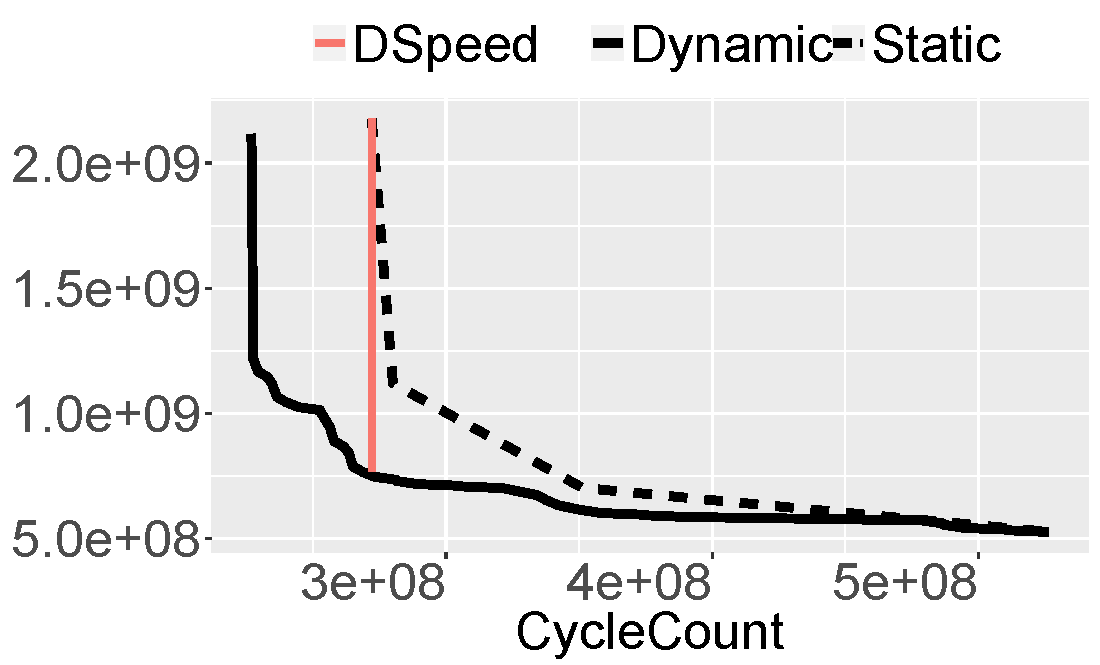
\includegraphics[width=0.3\textwidth]{cases-paper/graphics/Pareto/LocN3.pdf}\vspace*{-4mm}\label{subfig:loc}}
     \subfloat[][MSER]{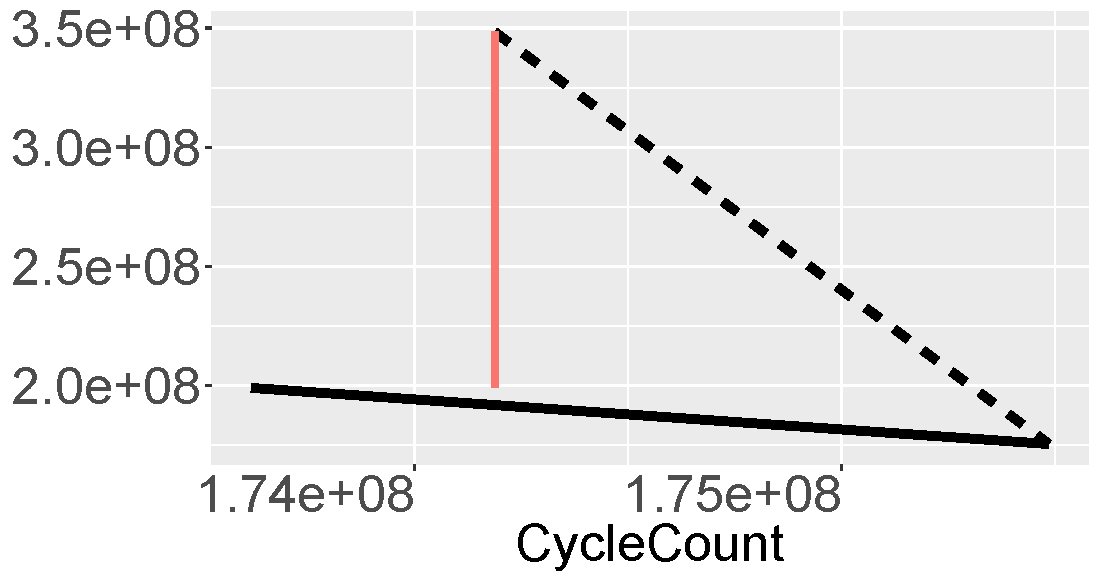
\includegraphics[width=0.3\textwidth]{cases-paper/graphics/Pareto/MSERN3.pdf}\label{subfig:mser}}\
	 	 	 \vspace{-0.5em}

     \subfloat[][Multi\_Ncut]{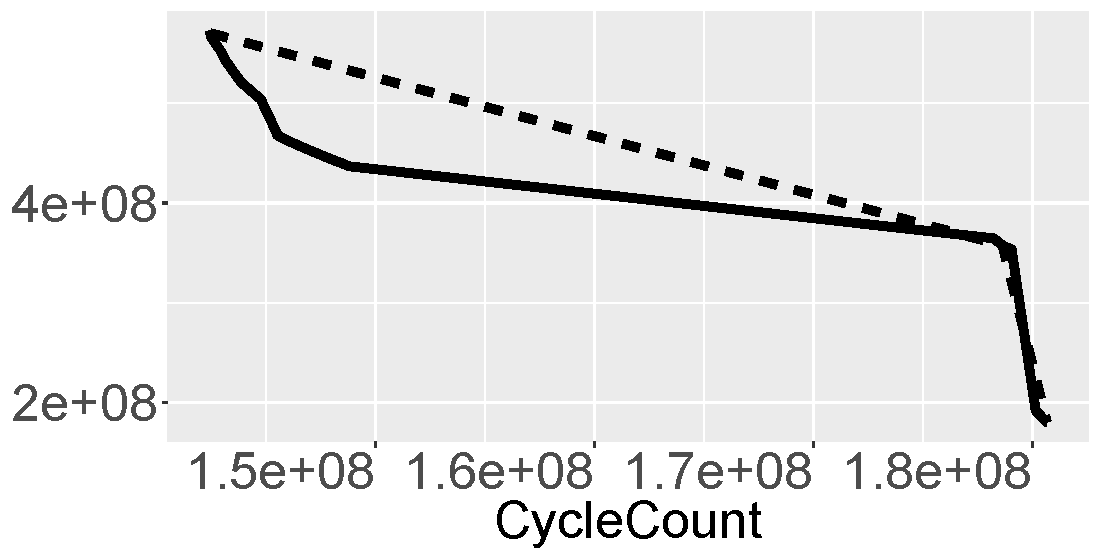
\includegraphics[width=0.3\textwidth]{cases-paper/graphics/Pareto/MultiN3.pdf}\label{subfig:mult}}
     \subfloat[][Sift]{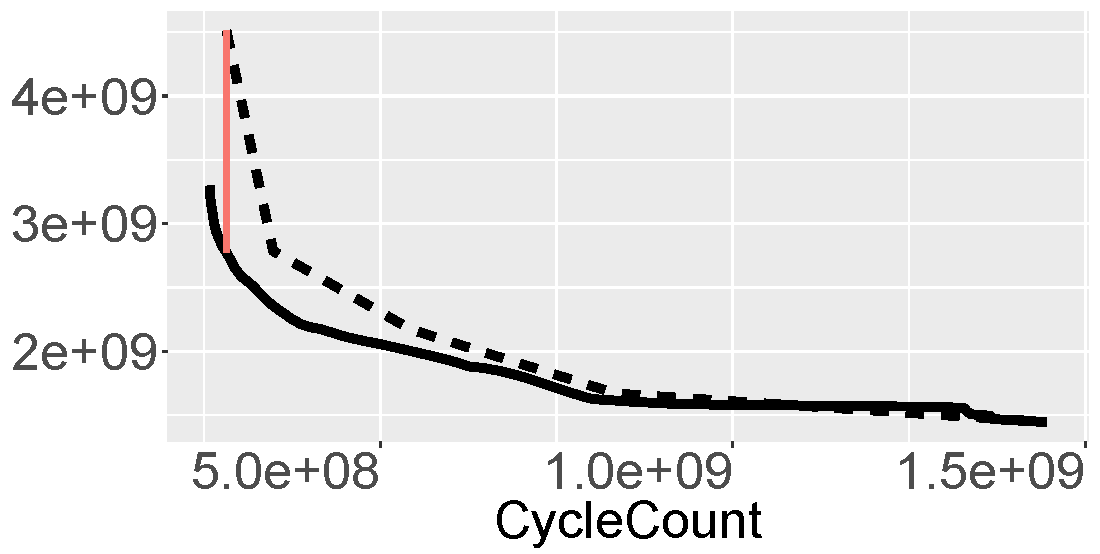
\includegraphics[width=0.3\textwidth]{cases-paper/graphics/Pareto/SiftN3.pdf}\label{subfig:sift}}
     \subfloat[][Stitch]{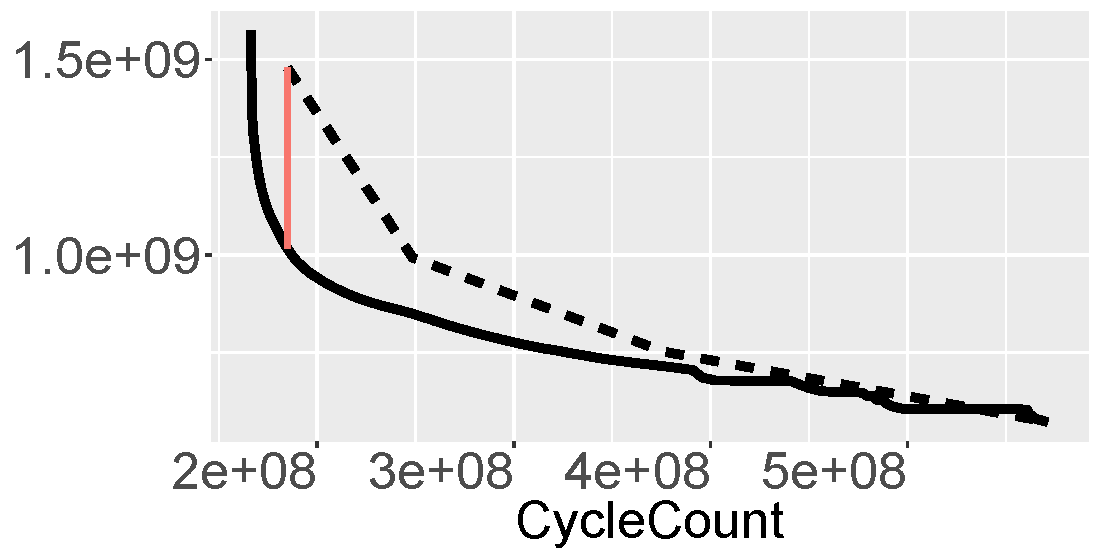
\includegraphics[width=0.3\textwidth]{cases-paper/graphics/Pareto/StitchN3.pdf}\label{subfig:stitch}}\
	 	 	 \vspace{-0.5em}

     \subfloat[][SVM]{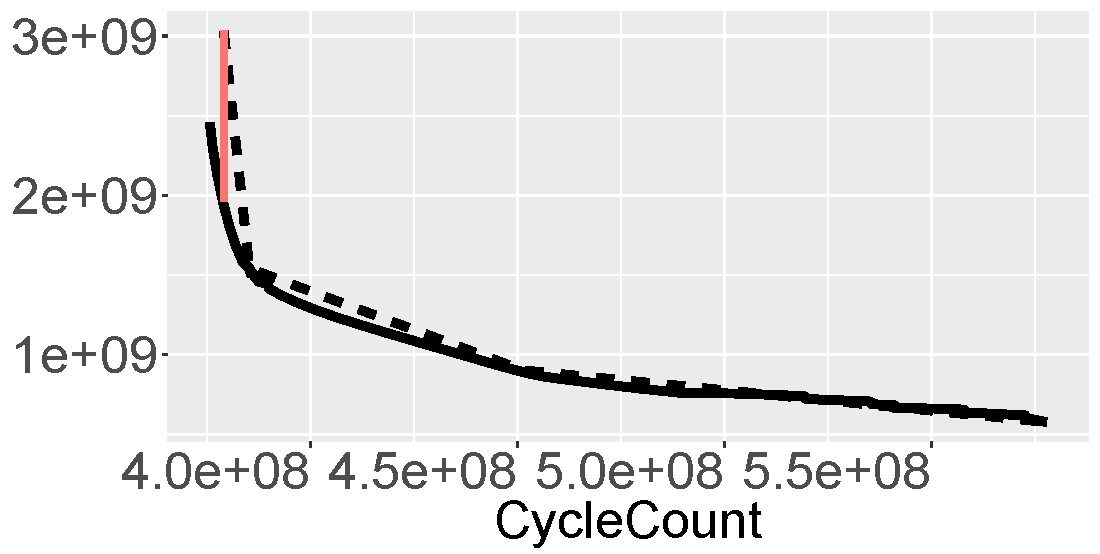
\includegraphics[width=0.3\textwidth]{cases-paper/graphics/Pareto/SVMN3.pdf}\label{subfig:svm}}
     \subfloat[][Texture\_Synthesis]{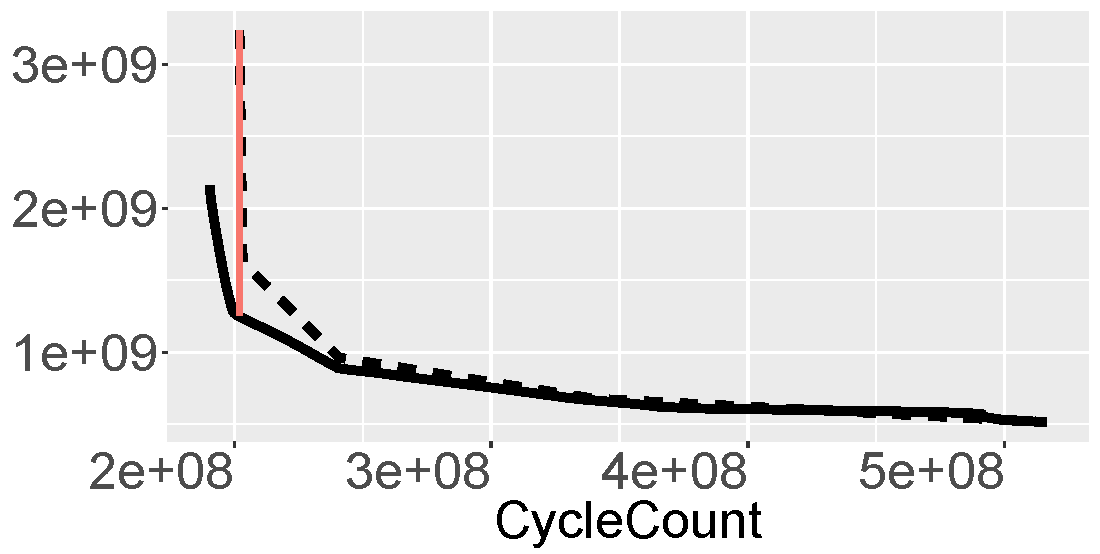
\includegraphics[width=0.3\textwidth]{cases-paper/graphics/Pareto/TextN3.pdf}\label{subfig:text}}
     \subfloat[][Tracking]{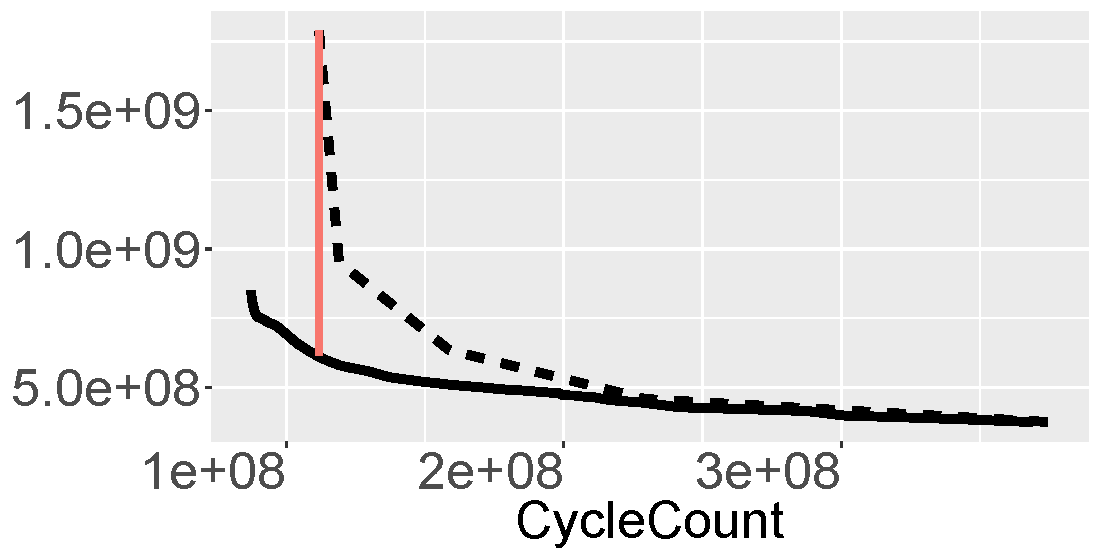
\includegraphics[width=0.3\textwidth]{cases-paper/graphics/Pareto/TrackingN3.pdf}\label{subfig:track}}
     \caption{Time (x-axis) vs. Energy (y-axis) tradeoffs using Static and Dynamic Composition Schemes.}
     \label{fig:paretos}
	 	 	 	 \vspace{1em}
\end{figure}

\subsection{Dynamic Core Fusion}
Figure~\ref{fig:paretos} shows the trade off between time (represented in cycles) and energy using either a static ahead of time configuration or a dynamic reconfiguration.
The dotted line represents the static core fusion scheme whilst the solid line represents the Pareto Front of all the dynamic core fusion traces.
The vertical line represents the amount of energy that can be saved from using a dynamic core fusion scheme that matches the same speed as the best static scheme.
The Pareto Front is constructed by assigning different LC sizes to a phase and recording the execution time in cycles and energy consumption.
For a given cycle count, the reconfiguration scheme that leads to the smallest energy consumption is chosen to be a point in the Pareto Front.

Figure~\ref{fig:paretos} demonstrates how static core-composition fails to maintain good energy efficiency as speed is improved.
For example, \bm{Disparity} (Figure~\ref{subfig:disp}) is fastest on 16 fused cores, but has an 1.63x increase in energy consumption for a 1.22x improvement in speed.
This is due to the fact that larger core-compositions do not result in linear speedups, and thus consume more energy than a smaller core-composition.
When using the dynamic scheme, it is clear that energy consumption increases at a slower rate when increasing speed.
In this case the number of cores is adapted to the current program phase, using just enough cores to maintain high performance without wasting energy.

Figure~\ref{fig:paretos} also shows how very few applications get faster execution times with dynamic core fusion.
The main program that does perform better execution wise with dynamic core fusion is \bm{Localization}.
In the case of \bm{Localization}, the fastest execution time using static core-composition comes from a logical core of size 8.
However, there are certain phases that will perform better with 16 cores, and thus, dynamic core fusion in this situation can lead to faster execution times.
Yet, overall for these benchmarks, most will have their fastest execution times with a static core-composition.
Dynamic reconfiguration is therefore mainly used to limit the energy consumption.

\begin{figure}[t]
    \centering
	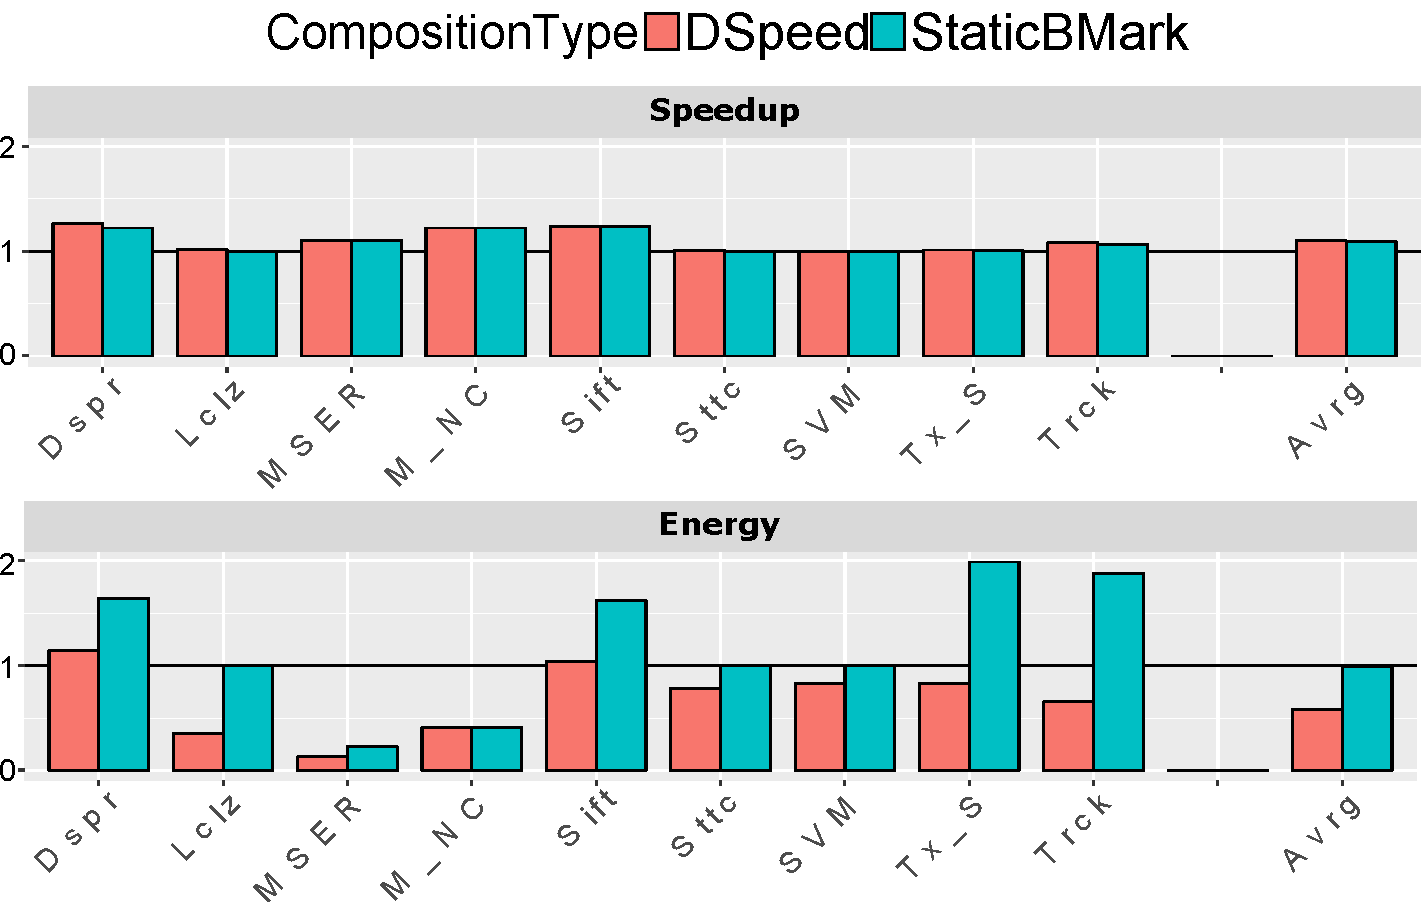
\includegraphics[width=1\textwidth]{cases-paper/graphics/results/speed_bars2.pdf}
    \caption{Maximizing speed for all the SD-VBS benchmarks. For Speedup, higher means better, for Energy, lower is better.}
    \label{fig:speedres}
	\vspace{1em}
\end{figure}

\subsection{Optimizing for Speed} \label{sec:dyn:speed}

In this section the dynamic scheme is defined to be one that matches the same speed performance as the fastest static core composition for the benchmark: \textbf{DSpeed}.
This is equivalent to the vertical line found in Figure~\ref{fig:paretos}.
This scheme is used to demonstrate how dynamic reconfiguration can outperform static configuration on a baseline of execution time.

Figure~\ref{fig:speedres} shows the speedup of \textbf{DSpeed} and Static Best (SB) and the respective energy consumption.
The results are normalized against the performance of Static Suite (SS), which is 8 cores fused.
The SS core count is obtained by averaging the number of cores that leads to the fastest execution time for each benchmark.
The execution times for \textbf{DSpeed} and SB are the same as the dynamic scheme is designed to match the static best's execution time.
As can be seen some benchmark perform better when using benchmark specific core fusions rather than SS.
Both \bm{Disparity} and \bm{Sift} obtain a 1.25x speedup when using the SB scheme whilst \bm{Tracking} benefits from a 1.10x speedup.
This reconfirms the concept that even static core-composition is a feature that leads to performance improvements over design time configurations.

When looking at the Energy graph of Figure~\ref{fig:speedres}, it is clear where the SS scheme fails.
Benchmarks \bm{MSER} and \bm{Multi\_NCut} feature very little improvements when using core composition, if any, therefore the SS will perform very poorly when it comes to energy consumption for the benchmarks.
In the case of those benchmarks, the energy consumption is over 2x less on SB than it is on SS.
In this situation, SS is analogous to designing a large physical core meant to extract a lot of IPC for single-threaded performance and executing low IPC benchmarks on it.
This kind of core will end up consuming too much energy and lead to low performance increases.
SB already shows the advantages of designing smaller, simpler physical cores which can be composed ahead of time.
For applications such as \bm{MSER} or \bm{Multi\_NCut}, a single low energy core will suffice whereas \bm{Disparity} and \bm{Tracking} can benefit from large compositions for better speedup.

However, SB is still not an optimal solution. 
For the benchmarks \bm{Disparity}, \bm{Sift}, \bm{Texture\_Synthesis} the energy consumption is much higher.
This is due to the fact that these benchmarks perform best on a 16-core system, however as seen in Figure~\ref{fig:stddev}, the variation in performance always increases when fusing this many cores.
In this situation, whilst 16 cores does result in the fastest execution times, the energy consumption is higher than SS.
This shows the limitations of static configurations overall, whether it be at design time or ahead of time: the lack of flexibility means that compromises have to be made.
In the case of optimising for speed, the compromise comes at the cost of energy consumption.

%More here
The dynamic reconfiguration \textbf{DSpeed} scheme always performs better than the SB scheme in terms of energy consumption and can even match the SS scheme on energy consumption whilst improving speed such as in the \bm{Sift} benchmark.
For the \bm{Localization} benchmark, the \textbf{DSpeed} matches the performance of both the SB and SS whilst reducing energy consumption by 65\%.
Overall, by using \textbf{DSpeed}, the energy consumption can be reduced by 42\% compared to both SB and SS without impacting performance.
This illustrates the greatest advantage of using a DMP since the number of fused core can be adapted continuously depending on the amount of ILP available for each phase.


\begin{figure}[t]
    \centering
    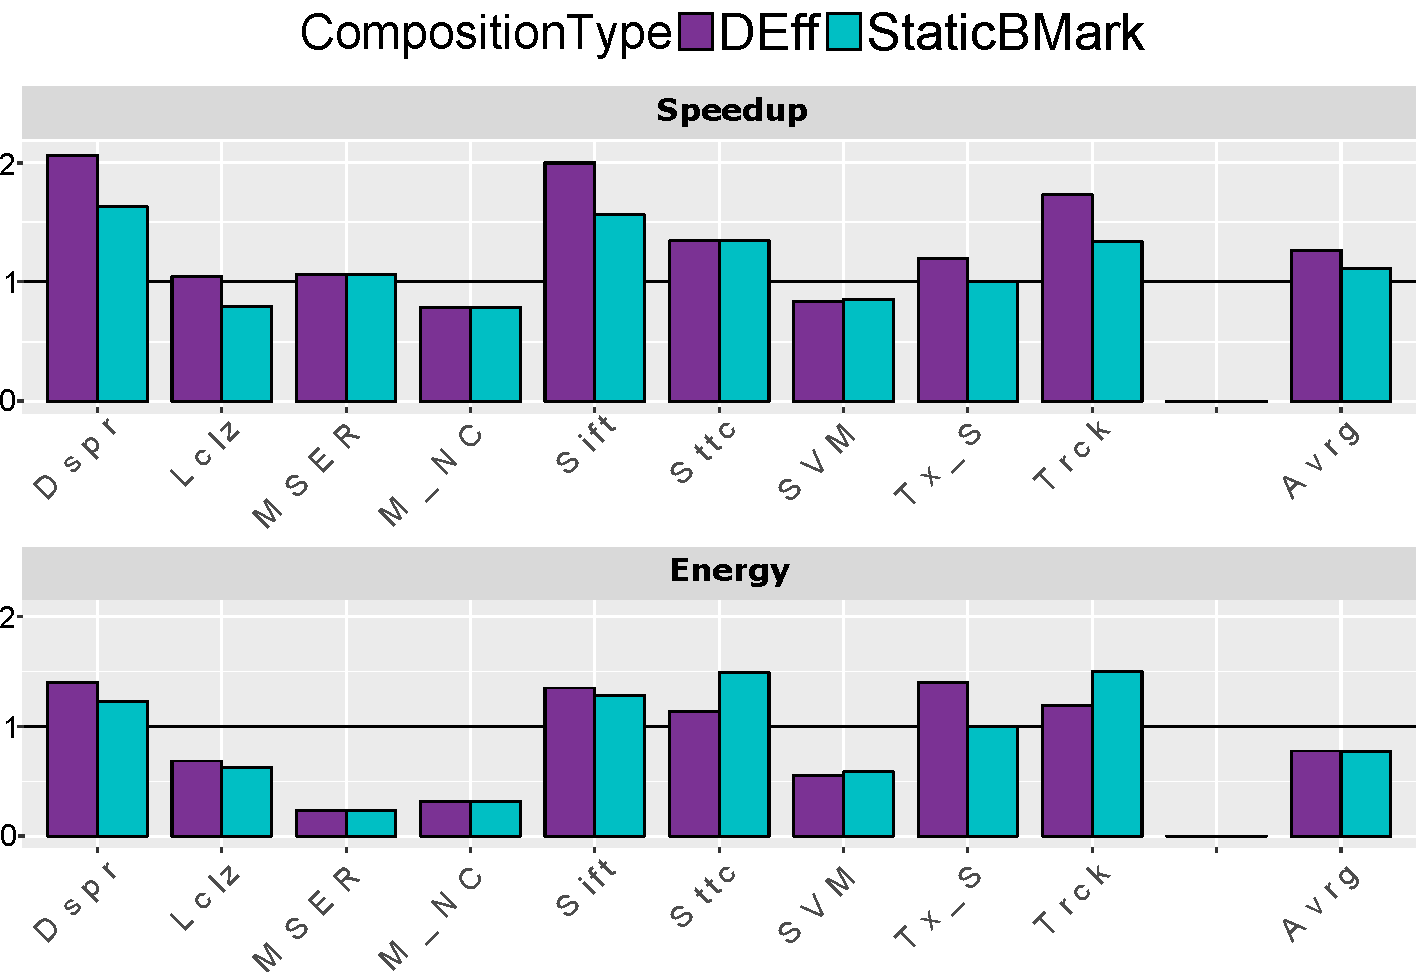
\includegraphics[width=1\textwidth]{cases-paper/graphics/results/edd_bars2.pdf}
    \caption{Maximizing efficiency for all the SD-VBS benchmarks. For Speedup, higher means better, for Energy, lower is better.}
    \label{fig:effres}
	\vspace{1em}
\end{figure}

\subsection{Optimizing for Efficiency}

%Cite how to get it, maybe put this in background as well.
This section defines a dynamic scheme that maximizes the efficiency metric EDD, which is defined as $Energy \times Delay \times Delay$ where Delay is the execution time (in cycles).
This metric attempts to optimize speed whilst remaining energy efficient.
In this section, the dynamic scheme that is optimised for EDD is called \textbf{DEff}.
The aim of generating a second dynamic scheme is to demonstrate that dynamic reconfiguration can be used to target different requirements.
Figure~\ref{fig:effres} shows the speedup performance of \textbf{DEff} and SB and their respective energy consumption.
The results are normalized against SS which is a fixed-composition of 4 fused cores.

%Once again start with SS/SB then introduce DEff

First, when comparing the SS and SB, the SB scheme is able to extract more speed whilst still being able to minimize energy consumption.
Once again, when it comes to energy the flexibility of SB over SS is mostly seen in \bm{MSER} \bm{Multi\_NCut} as both applications don't benefit from core composition.
In fact, optimising for EDD shows that the SB scheme can save energy for even more benchmarks, such as \bm{Localization} and \bm{SVM} without slowing down execution time.
Unlike the scenario where the processor is optimising for speed, SB can be faster than SS in this situation.
This is because for applications such as \bm{Disparity} and \bm{Sift}, the number of cores required to maximise \textbf{DEff} is larger than the SS scheme's: 8 cores vs 4 cores.
For these benchmarks, SB is 1.5x faster than SS whilst consuming less than 1.2x the amount of energy, thus being more efficient than SS.

Once again, when dynamic reconfiguration is taken into account, as seen by the \textbf{DEff} bars in Figure~\ref{fig:effres} it demonstrates the limitations of static configurations.
For benchmarks \bm{Disparity}, \bm{Sift} and \bm{Tracking} the \textbf{DEff} scheme is 1.30x faster than the SB scheme and at least 1.75x faster than the SS scheme.
It is important to note that this extra speedup does not incur great increases in energy consumption compared to SB: only 1.10x for \bm{Disparity} and \bm{Sift}.
In fact, for \bm{Tracking} \textbf{DEff} saves 20\% in energy compared to SB.
When comparing to SS \textbf{DEff} is 1.75x times faster for only 19\% more energy for the \bm{Tracking} benchmark.

Overall, \textbf{DEff} results in a 1.25x speed increase compared to SB and SS whilst consuming 25\% less energy than SS.
This shows how dynamic core fusion's flexibility allows us to get better speedups whilst not drastically increasing the energy consumption.

\subsection{Reconfiguration Latency} \label{sec:reconfoverhead}

%Check if th
Up until now, the chapter has assumed a reconfiguration latency of 100 cycles whenever dynamic reconfiguration occurs as explained in the background chapter, Chapter~\ref{chp:Background}.
This section studies the impact of a larger reconfiguration overhead on energy savings.
First, figure~\ref{fig:avlen} shows the average phase length for each benchmarks when maximizing energy savings while maintaining performance (\textbf{DSpeed}).
As can be seen, the majority of the benchmarks run for long period of several ten of thousands cycles before any switching occurs.
Therefore, even if the reconfiguration latency would be increased to larger value (\eg 1,000 cycles), its impact might be minimal.
%Free line, will need to give more info in the input section
For these benchmarks, the phase length is also tied to the size of the input, thus the phases will increase when working on larger inputs such as high definition images.

Furthermore, there is always the option to reconfigure less often, in the case where a change in configuration only brings marginal reduction in energy.
In such case it might be more beneficial to keep running on the slightly less optimal configuration than paying a cost for reconfiguration.
Figure~\ref{fig:enlatency} illustrates perfectly this scenario, showing how energy behaves as a function of the reconfiguration overhead (averaged across benchmarks).
For each latency value, the best trace of reconfiguration is determined to keep performance constant while minimizing energy (\textbf{DSpeed}).
The left y-axis expresses the energy savings relative to the static scheme, while the right y-axis shows the total number of switches.
The energy savings remains high up to a latency of 1,000 cycles, with a noticeable decrease in the number of switches.
For latency values over 1,000 cycles, the energy savings drop considerably, with very few switching occurring.
This data shows that even if the reconfiguration overhead is 1,000 cycles, average energy savings of 38\% are possible compared to 42\% when the overhead is 100 cycles.

\begin{figure}[t]
    \centering
	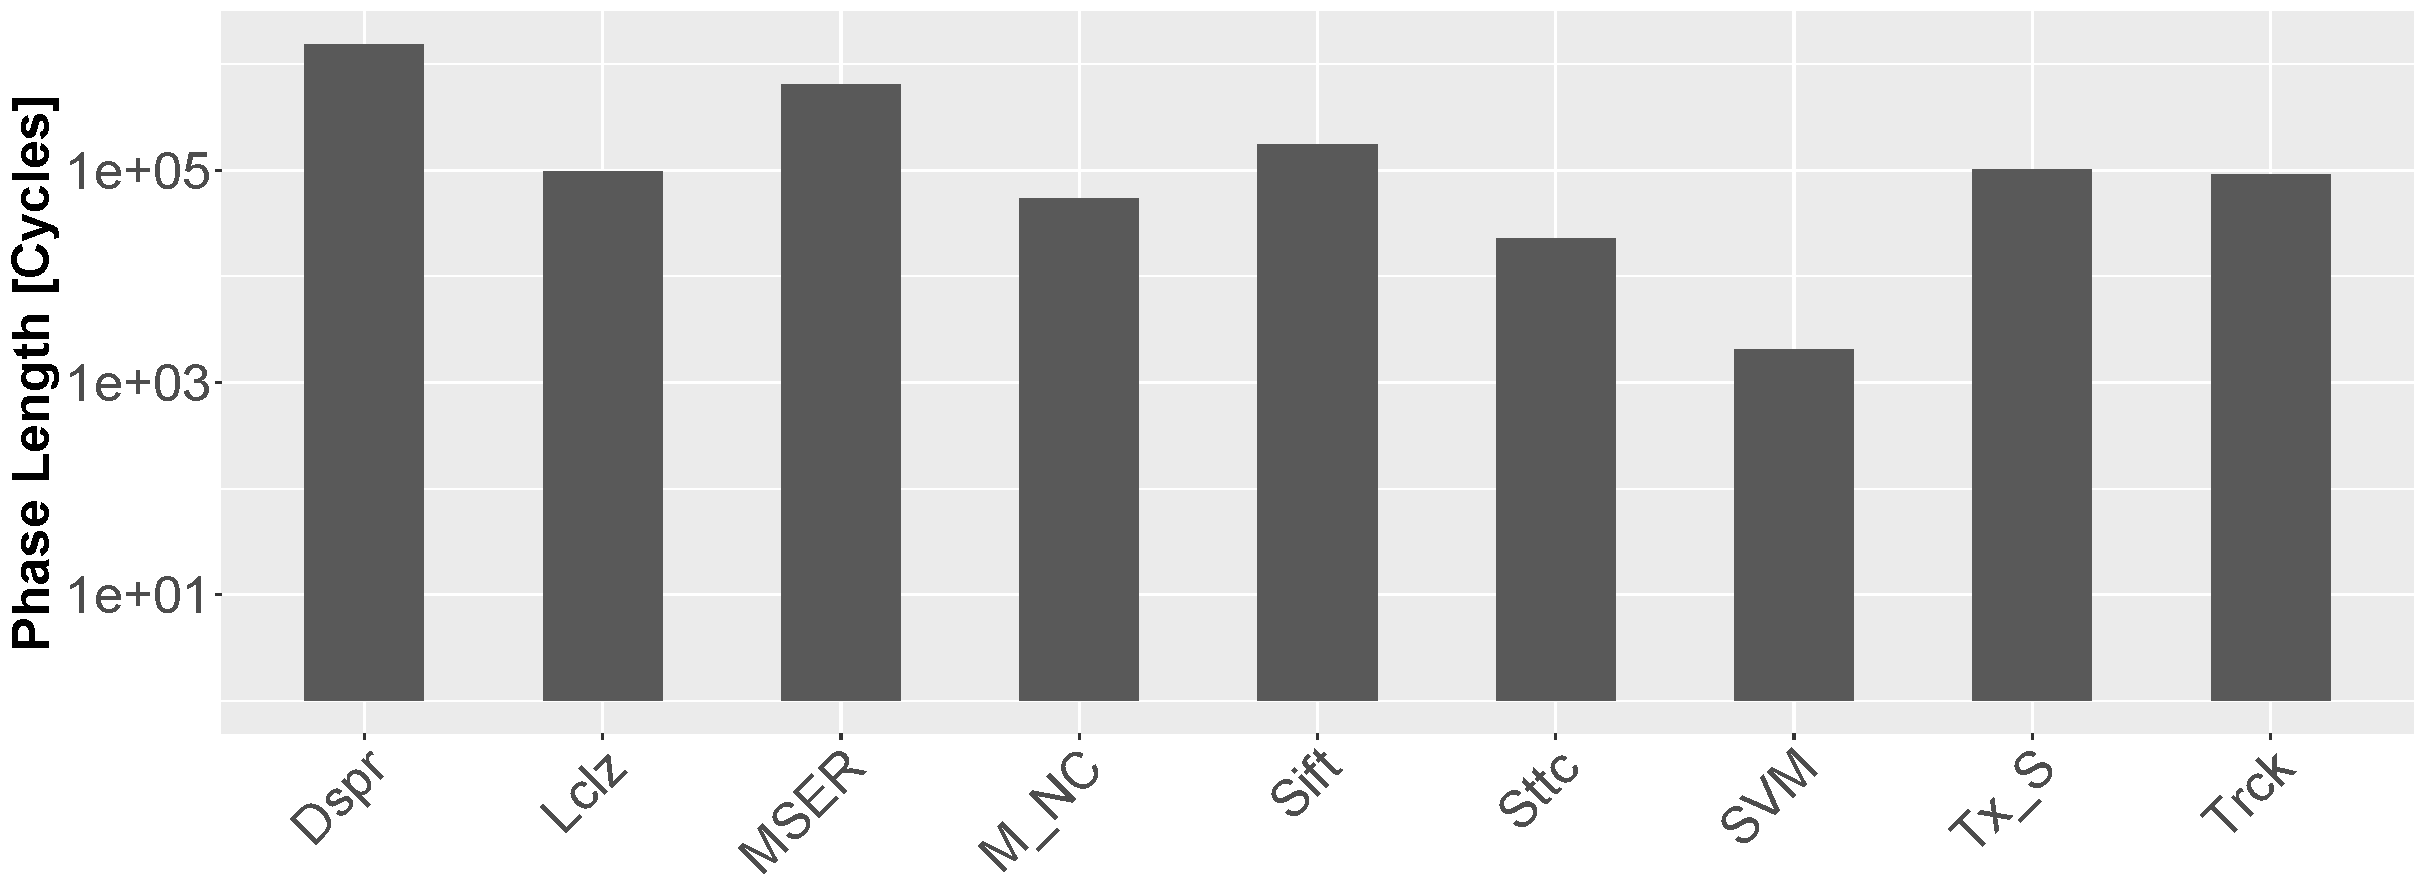
\includegraphics[width=\textwidth]{cases-paper/graphics/Exploration/phase_len2.pdf}
    \caption{Average number of cycles without switching.}
    \label{fig:avlen}
\vspace{1em}
\end{figure}
\begin{figure}[t]
\centering
	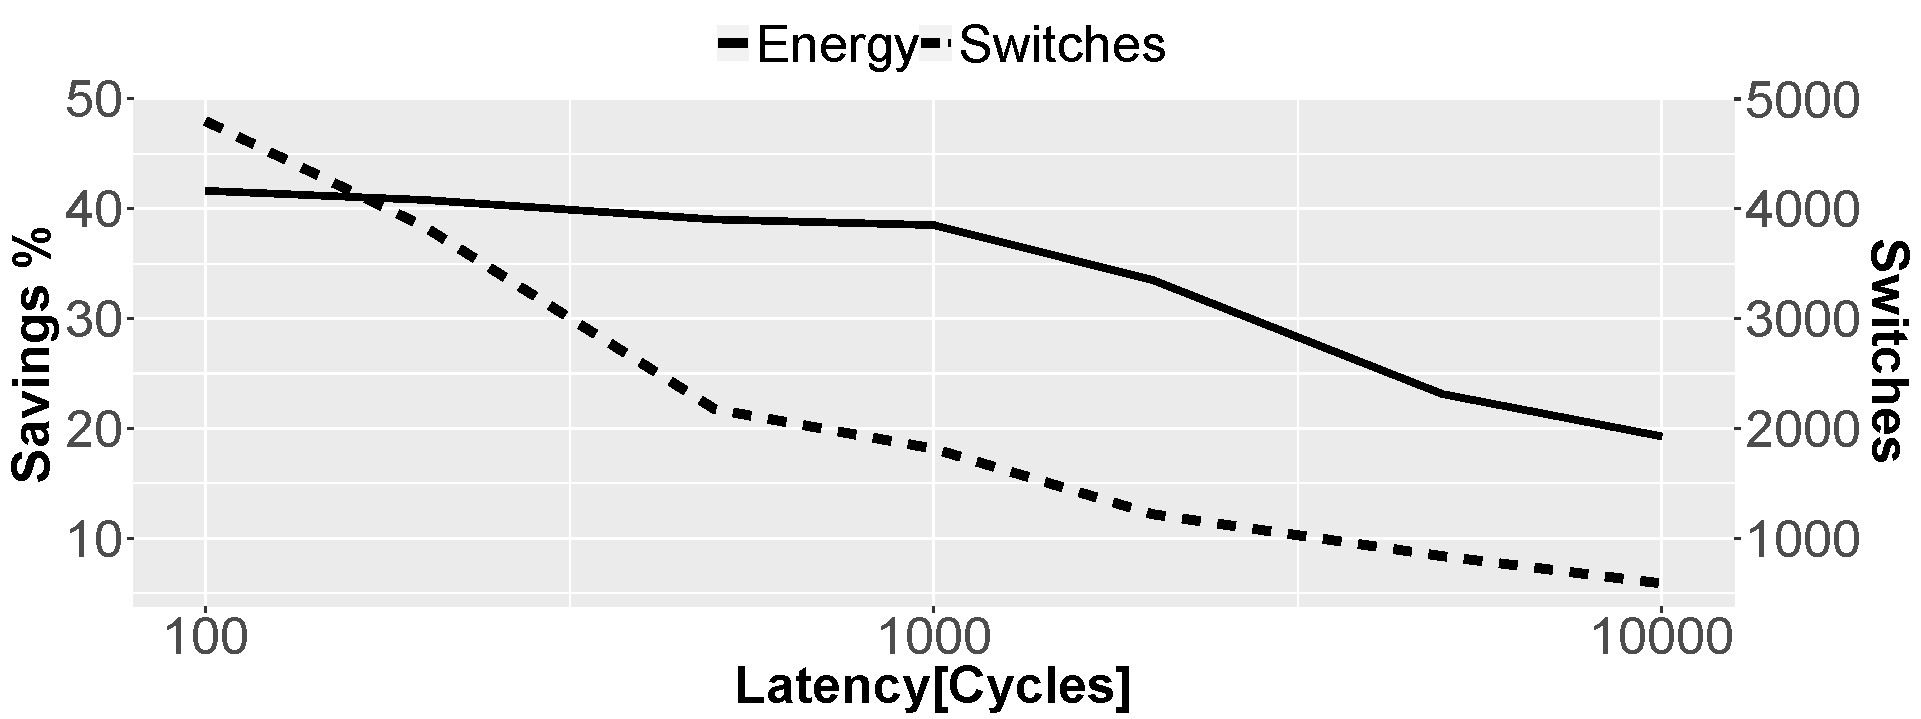
\includegraphics[width=\textwidth]{cases-paper/graphics/Exploration/latency_en_sp_sw2.pdf}
    \caption{Energy savings and number of switches as a function of the switching latency in cycles.}
    \label{fig:enlatency}
\vspace{5mm}
\end{figure}

\paragraph{Summary}

Overall, whether the program is optimize for speed or efficiency, dynamic core fusion will always lead to higher speedup or lower energy consumption than a fixed configuration.
This is due to the presence of phases in applications that the dynamic scheme can exploit to reduce wasting energy in low ILP phases.
This section has shown that maximizing speed can be highly energy inefficient when using a static LC and that a dynamic scheme can help reduce energy consumption by 42\% on average.
When optimizing for efficiency, the section demonstrates that a dynamic scheme can help improve both speed and energy consumption, for example in the case of \bm{Tracking}, and overall speed can be improved by 1.25x whilst saving 25\% energy.




\section{Linear Regression Model}\label{sec:model}
The previous section showed that dynamically reconfiguring the processor can help reduce energy consumption whilst still achieving the same execution time as the fastest ahead of time configuration.
In order to benefit fully from dynamic core-composition two solutions are possible; either the programmer must go through the code and manually determine when to change the composition or an automatic scheme can be deployed.
This section now presents a learning scheme that is used to exploit the large energy savings available.
The main idea is to monitor at runtime some performance counters and make a decision at a regular interval on how to reconfigure the cores.
For this purpose, a model is trained offline using the data collected and presented earlier in the chapter.
Once trained, the model predicts the optimal number of cores based on the performance counters from the previous time interval and reconfiguration occurs if it is different from the current number of cores.

\begin{figure}[t]
    \centering
	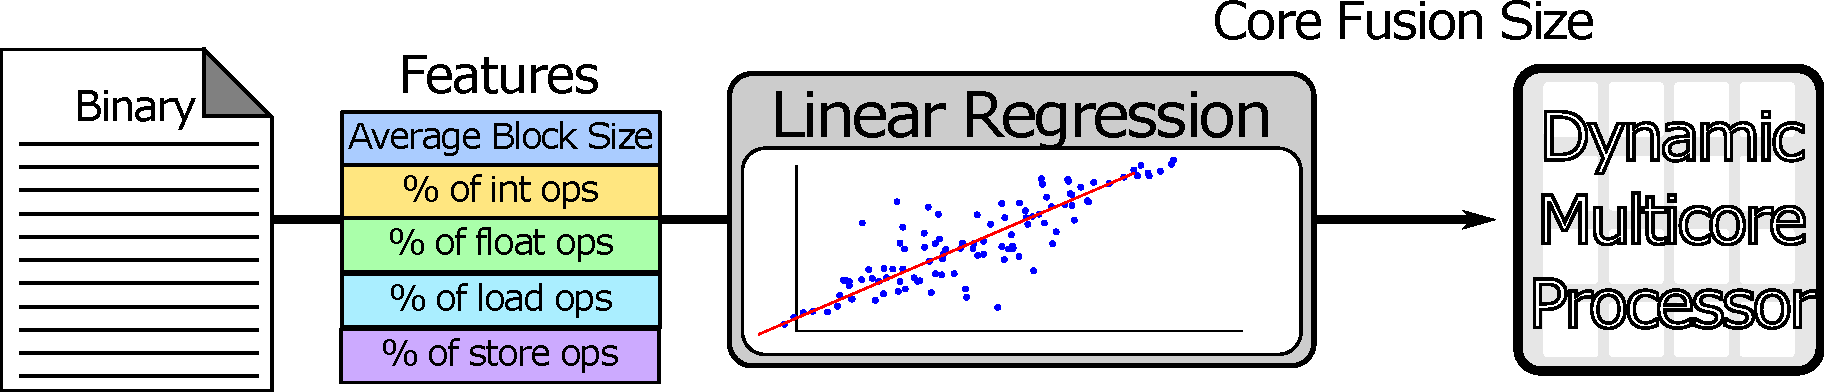
\includegraphics[width=1\textwidth]{cases-paper/graphics/other/model3.pdf}
	\vspace{-2em}
    \caption{Linear Model.}
    \label{fig:linmod}
\end{figure}
\subsection{Model}

As the decisions are made at runtime, a lightweight model that is able to predict the correct configuration that can be integrated in hardware is necessary.
Linear regression, which makes predictions using a weighted sum of the input feature, has been demonstrated to be useful for predicting processor performance~\cite{Joseph2006LinReg}.
It is chosen as it has been as it can easily be implemented in hardware~\cite{lee2006linreg,Lukefahr2012Composite} and has a low overhead when computing the sum.
The model is trained offline using the traces gathered from the prior analysis for the \textbf{DSpeed} scenario which maximises energy savings while maintaining performance.

Figure~\ref{fig:linmod} is a shows how the linear model is trained.
The dataset consists of a set of four input features (average block size, and percentage of integer, floating point and load operations) and the optimal number of cores for each time tick for each program.
These features are chosen as they are easy to extract from the hardware.
The reason stores are not in the feature vector is due to the fact that a block is comprised only of integer, floating point, load and store operations.
Therefore, when building the model, a correlation analysis determined that stores correlate with other features and selects to remove it as a variable.
 % a single data point is created per phase, averaging the features of all the ticks in a phase, resulting in a total of 34 pairs of optimal core number and features.

To speedup the learning process, for each benchmark the features of all the ticks in a phase were averaged out to create a single data point, which is comprised of an IPC value, and the features described in Figure~\ref{fig:linmod}.
This averaging out leads to 34 data points for all the benchmarks.
The training consists of finding the weights that minimise the error when predicting the optimal number of cores to use across all time ticks and benchmarks.
Since only core configurations which use a power of two number of cores are considered, the linear model is built to predict the logarithm (base 2) of the number of cores.
The prediction is rounded up to the nearest integer in the interval $[0,4]$.
The following equation represents the trained linear model which can be used to make prediction:
\vspace{-1em}
\begin{align*}
  log_2(\textbf{\#cores}) = & -7.7\ +\ 0.028 \cdot \textbf{avgBlkSze}\ +\ 0.075 \cdot \textbf{\%int\_ops}\ +\\
 &0.069 \cdot \textbf{\%fp\_ops}\ +\ 0.21 \cdot \textbf{\%ld\_ops}
\end{align*}

It is important to note that this model was not used during the validation, as cross-validation (see Chapter~\ref{chp:Background}) was used to evaluate it.
Instead, this represents a model where the data from all programs is used.
For instance, if at runtime an average block size of 6 instructions, and 77\%, 1\% and 18\% of integer, floating point and load operations, respectively, then the predicted value will be 2.092.
Rounded up to the nearest integer value, 2, the optimal number of cores predicted will, therefore, be 4.

As can be seen, the largest weight is on the percentage of loads operations.
This is due to different reasons, mainly execution time and the fact that Load-Store Queues are fused.
When it comes to execution time, loads may take from 3 to 128 cycles depending on whether or not it is a cache miss or hit.
Whether it is a cache hit or miss, a block that takes longer to execute will often minimise the \textit{SynchronisationCost} penalty.
A block composed mainly of integer or floating point operations will often result in shorter execution rates; thus may execute faster, making it harder for large logical cores to improve performance.

More discussion on how the time it takes to execute a block influences the performance of core compositions is discussed in Chapter~\ref{chp3}.
The other reason loads have the largest weight is due to the fact that loads can be fired independently to the Load-Store Queue.
Unlike stores that depend on previous memory instructions blocks being committed, loads can be fired with less overhead.
As data can be speculatively fetched, load instructions can receive data from other cores before the data is stored, speeding up executions.
By increasing the core count on load heavy blocks this will improve performance more reliably due to cores being able to issue loads in parallel.

\begin{figure}[t]
    \centering
	\includegraphics[width=1\textwidth]{cases-paper/graphics/results/lr_speed3.pdf}
    \caption{Performance results for maximising speed for the SD-VBS benchmarks using the linear regressor (LR) model. The results are normalised against the Static Suite core composition.}% For Speedup, higher means better, for energy lower is better.}
    \label{fig:speedlr}
	\vspace{1em}
\end{figure}

%explain why MSER here is bad. Most likely because it over-estimates because some features in the vector don't describe the performance in the application.
%This is most likely due to the branch prediction/.
\subsection{Results}

To evaluate the performance of the model leave-one-out cross-validation  is used; it is a standard machine-learning methodology which tests the model using not seen during training.
For instance, if the model is tested for one program, let say \textit{Disparity}, the model is then trained using the dataset from all the other programs combined.
Then the resulting trained linear model is used to predict the optimal core number for each time tick of the disparity program and report the performance achieved.

Figure~\ref{fig:speedlr} shows the performance in terms of speed and energy that is achieved using the linear model normalised by a fixed static configuration.
The fixed configuration maximised performance across all the benchmarks using 8 cores and is the same as in the previous results presented in figure~\ref{fig:speedres}.
On average, the linear regressor model is able to consume 37\% less energy compared to the 8 cores fixed configuration and is able to exactly match its speed.
The main outlier is \bm{MSER} where the linear regressor consumes over 2x more energy than \textbf{DSpeed}.
This is due to the fact that \bm{MSER} is a benchmark where the branch prediction is poor as previously mentioned in Table~\ref{tab:sd-vbsbpred}.
Indeed, \bm{MSER} has an average branch prediction of 85\% compared to the average of 95\%.S
As \bm{MSER} tends to have very small blocks, the branch prediction makes it very difficult to ever efficiently use even a core composition of size 2.
This benchmark is therefore an outlier compared to the rest of the set, as it is the branch prediction causing incorrect predictions from the linear regression.

The performance is also compared with the best possible choice of dynamic reconfiguration, \textbf{DSpeed} which acts as an Oracle.
As can be seen, the linear model is able to exploit similar energy savings to the \textbf{Dspeed} scheme in most cases.
On average it reduces energy by 37\%, which is within 5\% of the 42\% achievable by the \textbf{Dspeed} scheme.
These results show that it is possible to implement a simple realistic lightweight scheme which offers large energy savings.


%\section{Related Work}\label{sec:related}
%
\paragraph{Reconfigurable Processors}

ElasticCore~\cite{tavanaElastic} proposes a morphable core that uses dynamic voltage and frequency scaling (DVFS) and microarchitectural modifications such as instruction bandwidth and capacity.
They propose a linear regressor model to determine reconfiguration, which uses more runtime information than ours, such as branch prediction and cache misses.
Overall Tavana et al's architecture is 30\% more energy efficient than a big.LITTLE architecture.

In~\cite{dubach13dynamic} they also propose a similar core architecture that modifies microarchitectural features.
They provide extensive analysis of SPEC 2000 benchmarks and demonstrate that machine learning and dynamic adaptation can double the energy/performance efficiency compared to a static configuration.

MorphCore~\cite{khubaibMorphCore2012} focuses on reconfiguring a core for thread level parallelism.
It switches between out-of-order (OoO) when running single threaded applications and an in-order core optimised for simultaneous multi threading (SMT) workloads.
This provides an opposite solution to our DMP: providing a large core made for ILP that can be modified to better fit TLP workloads.
MorphCore outperform a 2-Way SMT OoO core by 10\% whilst being 22\% more efficient.

All these projects focus on uni-core modifications, and traditional CISC/RISC like architecture which differs from our work.

\vspace{-0.5em}
\paragraph{Dynamic Multicore Processors}
Previous work on Dynamic Multicore Processors includes CoreFusion~\cite{ipek2007CoreFusion} and Bahurupi~\cite{pricopi2012bahurupi,pricopiSchedCoreComp2014}.
These architectures use a standard ISA and either fetch fixed sized instruction windows~\cite{ipek2007CoreFusion} or entire basic blocks~\cite{pricopi2012bahurupi}.
Other DMPs such as TFlex~\cite{kim2007tflex} and E2~\cite{e2} use an hybrid-dataflow EDGE ISA~\cite{burger04edge}. 
In TFlex, instructions from a block are executed on different fused cores.
In E2, a block is mapped to a fused core and all instructions from that block execute locally.

\vspace{-0.5em}
\paragraph{Dynamic Core Fusion}
In the work of Pricopi {\it et al.~}~\cite{pricopiSchedCoreComp2014}, they show how dynamic reconfiguration is beneficial when it comes to scheduling tasks.
However, they do not discuss any method of automatically deciding the optimal configuration beyond a 4 core fusion.
Instead they use speedup functions determined from profile executions of applications to determine how to schedule tasks.
They do not discuss what software characteristics help determine when to reconfigure the cores, or how to optimise software.

Work on using machine learning to automatically choose a composition was achieved in~\cite{micolet2016dmpstream}.
This work does not involve changing the core fusion dynamically during the execution of the benchmark.
The machine learning model focuses on using high-level information from StreamIt's~\cite{thiesStreamit2010} language constructs.

\vspace{-0.5em}
\paragraph{Voltage Scaling}
Voltage scaling is another method of reducing energy consumption~\cite{paganiEECHM2017}, however this approach is orthogonal to DMPs~\cite{sibi}.
Whilst both methods adapt to programs phases, DMPs can also be used to speed up the execution of programs.


\section{Conclusion}\label{sec:conc}
This chapter tackled the problem of dynamic reconfiguration of a Dynamic Multicore Processor at runtime.
Due to the fact that adding cores in a core composition does not result in linear improvements, obtaining the fastest performance comes at the cost of energy.
Therefore using ahead of time static core compositions is not an efficient way of speeding up programs with phases as energy consumption will be high when executing phases with low IPC. % static core compositions are not an efficient method to speed up programs with phases.
Runtime dynamic reconfiguration of DMPs is therefore necessary to ensure that core compositions are used appropriately.

To better understand how core composition is sensitive to branch prediction and block size, a limit study has been conducted.
It showed that larger core compositions favour large blocks as this reduces the strain on the branch predictor and also reduces the communication cost between cores.
To improve the size of blocks and block level parallelism, a set of compiler optimisations such as loop inversion, loop unrolling and predication have been discussed.

These optimisation were then applied on a set of vision benchmarks, as they are programs that feature varying phases of IPC, and the performance of static core compositions help show that these programs have phases of IPC patterns.
Using this information, a dynamic runtime reconfiguration scheme was created:  \textbf{DSpeed} that matches the speed of the fastest static core fusion whilst minimising energy consumption.% and \textbf{DEff} that maximizes efficiency.
The chapter shows that \textbf{DSpeed} saves on average 42\% energy compared to the optimal static core composition core.% whilst \textbf{DEff} can improve performance by up to 1.30x and reduce energy consumption by 1.20x on some benchmarks.

Finally a linear regression model has been proposed to drive the adaptation process at runtime for \textbf{DSpeed}.
This  model leads to a 37\% reduction in energy whilst maintaining the same level of performance as the optimal static scheme.

Overall, the contributions of this chapter are:

\begin{itemize}
\item An analysis of the limits of core composition via an analytical model that demonstrated that in order for core composition to be effective, blocks must be large to reduce the strain on branch prediction accuracy and the cost of synchronising cores.
\vspace{-0.5em}
\item An in-depth comparison of static ahead of time and dynamic core composition schemes on the San Diego Vision Benchmark Suite which demonstrated that the benchmarks benefit most from dynamic core composition as it can achieve the same speedups as static ahead of time whilst reducing energy savings.
\vspace{-0.5em}
\item A demonstration that core composition has the potential to offer a large reduction in energy savings of up to 42\% compared to the static ahead of time core composition.
\vspace{-0.5em}
\item An analysis of how the cost of reconfiguring can affect the overall energy savings. The chapter showed that for the set of benchmarks, the reconfiguration cost can be as high as 1000 cycles without greatly impacting performance.
\vspace{-0.5em}
\item A demonstration that a linear-regression based model can predict the number of cores to fuse for different program phases using static code features and can achieve similar energy savings as the optimal execution with 36\% energy savings on average.
\end{itemize} 

%In this paper we have shown that whilst static core fusion already demonstrates promising results, it becomes harder to be efficient when increasing the size of logical cores.
%We explained theoretical limitations of static core fusion; without high branch prediction and large blocks, it under-performs.
%This was followed by a study of a suite of benchmarks, showing how performance varies greatly depending on the size of logical cores. 

%We then created two dynamic schemes: \textbf{DSpeed} that matches the speed of the fastest static core fusion and \textbf{DEff} that maximizes efficiency.
%Using these schemes we saw that \textbf{DSpeed} saves on average 42\% energy compared to the optimal static logical core for a given benchmark.
%We also showed that \textbf{DEff} can improve performance by up to 1.30x and reduce energy consumption by 1.20x on some benchmarks.
%Finally, we developed a simple linear regression model to decide on the number of cores to fuse at runtime to optimize for performance, leading to a 37\% reduction in energy while maintaining the same level of performance as a static scheme.



\chapter{Adapting hardware to improve core composition performance}

\section{Introduction}\label{sect:introduction-chapter3}
%replace the ref with actual latex ref
The previous chapter showed how reconfiguring a dynamic multicore processor at runtime can improve the efficiency of core composition as it is able to adapt to different phases of instructions per cycle (IPC).
It also demonstrated that there are certain limiting factors to how performant core composition can be.
The limiting factors discussed were branch prediction requirements and cost of synchronising cores.
To improve the performance of core composition, Chapters~\ref{chp:streamit} and ~\ref{chp:cases} showed that source level modifications are a good method.
These source-level modifications are often used to increase the size of the block which enables better utilisation of large core compositions.

Whilst source-level modifications do in fact improve the performance of large core compositions, they may not always be applicable.
In situations where source or compiler optimisations cannot increase the size of a block, core composition cannot improve the performance of the application.
To increase the viability of core composition, other solutions must therefore be explored.
Instead of solely focusing on improving the source code, analysing how a composition functions at a hardware level can help determine other potential bottlenecks in the system.

When modifications to software cannot yield any performance improvements, it is important to investigate if any hardware modifications can help increase the usefulness of core fusion.
By modifying how core composition behaves, this can potentially improve the performance on large compositions.
For example, modifying how blocks are distributed amongst cores can potentially increase the fairness of work distribution, increasing the efficiency of the composition.
This chapter explores the hardware bottlenecks that reduce the efficiency of core composition, and how to address these concerns.

There are two features of the processor that have a large impact on performance that are explored: first the block fetching mechanism in a composition, and data depenencies resolution between blocks can be handled.
The current fetching model focuses on filling the instruction window of a single core before activating another core in the composition.
Without modifications, this fetching model requires either large blocks to reduce the time required to activate multiple cores in a composition or a fast issue and dispatch width on the core, which increases the complexity of the design.
Thus, exploring how the fetching model can be modified to prioritise using all the cores in the composition over filling a single core can lead to better utilisation of the composition.

Secondly register dependencies can reduce block level paralellism which in turn makes core composition less useful.
Reduced block level parallelism due to data dependencies is similar to an issue found in superscalar processors~\cite{peraisBeBop2015}.
If register values could be predicted, instructions could fire speculatively which in turn would improve block level parallelism.
This chapter therefore explores how a value predictor, which predicts register values to reduce the data dependencies, can be used to improve performance in core composition.

This chapter is organised as follows: first a benchmark previously described in Chapter~\ref{chp:cases} is re-analysed to underline how current hardware does not suffice to ensure performance improvements.
Then a new fetching mechanism called Round Robin Fetch is introduced: cores are able to fetch blocks independently in a round robin fashion to improve fairness.
This is followed by a discussion of how value prediction can be used to resolve data dependencies between blocks and reduce performance penalties caused by the network on chip.
A current state-of-the art predictor is then discussed and shown to be applicable for the EDGE architecture.
Then an exploration of how these hardware modifications affect performance of core composition under an idealistic scenario, where perfect value prediction is enabled is conducted.
The benchmarks used in this chapter are the San-Diego Vision benchmark suite, the same as Chapter~\ref{chp:cases}.
Finally this is then followed by an evaluation of a real value predictor~\cite{peraisBeBop2015}, the block based differential VTAGE predictor (D-VTAGE).
Different parameters of the predictor are modified to understand how value prediction can be adapted to EDGE.

To summarise, the contributions are:

\vspace{-1em}
\begin{itemize}
\item A presentation of a new fetching scheme, Round Robin Fetch.
\vspace{-1em}
\item An analysis of how how value prediction can improve performance of core composition on the SD-VBS benchmark suite~\cite{sdvbs}.
\item An implementation and evaluation of the block-based VTAGE value predictor for EDGE, demonstrating that performance can be improved by only predicting register reads.
\end{itemize}
\section{Motivation}\label{sect:ch3-motivation}
This section explores how core composition performance depends on branch prediction, fetching mechanism, and data dependencies between blocks and how modifications to certain mechanisms can improve performance.
\vspace{-1em}
\subsection{Branch prediction}
\begin{figure}[t]
    \centering
    \includegraphics[width=1\textwidth]{chapter3/graphics/motiv_p1.pdf}
    \caption{Left: Speedup obtained when executing the MSER benchmark on different compositions and branch prediction accuracies.
	Right: Percentage of time (in cycles) cores in a composition execute instructions compared to the overall execution time. Higher is better for both.}
    \label{fig:mser_motiv}
    \centering
    \includegraphics[width=1\textwidth]{chapter3/graphics/perfect_fetch_motiv2.pdf}
    \caption{Speedup obtained when executing the MSER benchmark with different core composition with an oracle fetching scheme and perfect branch prediction. Higher is better. }
    \label{fig:motivation_fetch}
	\vspace{1em}
\end{figure}
Chapter~\ref{chp:cases} section~\ref{sec:lim_study} highlighted the importance of branch prediction accuracy when fusing a high number of cores.
To maximise utilisation, a core can have multiple blocks in its instruction window.
In this thesis, the instruction window is segmented into four lanes, each of which can hold a block of up to 32 instructions.
If the program executing mainly has small blocks, then if it is running on a 16 core composition, the branch prediction accuracy needs to be as high as 98\% to ensure that the cores are fetching blocks on the correct execution path (see Chapter~\ref{chp:cases} section~\ref{sec:lim_study}).

In Chapter~\ref{chp:cases}, \bm{MSER} had a low branch prediction accuracy of 85\%, leading to a performance improvement of only 1\% on a 2 core composition.
To see how difference accuracies affect performance, a branch predictor that can predict at different accuracy levels is used.
The left hand side of Figure~\ref{fig:mser_motiv} shows the speedup obtained when executing the SD-VBS benchmark \bm{MSER} on core compositions of size 2, 4, 8, 16 with different branch prediction accuracies on the cycle-accurate simulator.
The speedup is obtained by comparing the performance to a single core.
As the figure shows, increasing the accuracy to 100\% leads to a performance increase of 1.15x on a 16 core composition.


\subsection{Fetching mechanism}
The reason performance does not improve much is due to the fact that \bm{MSER} features small blocks.
Currently, when cores are composed, they fetch blocks in a serial fashion, as defined in Chapter~\ref{chp:Background} Section~\ref{chp:Background:sec:EDGE}.
As cores only submit fetch requests to other cores in the composition if they are full, this means that if a core is able to commit a block before being full, then it will never submit a fetch request to another core.
In this situation, cores in a composition may remain inactive during the execution of a program as they are not prompted to fetch blocks.
Throughout the rest of this chapter, this fetching scheme is referred to as Serial Fetch (SF).% (see Chapter~\ref{chp:Background} for more details).

To understand how the fetching scheme can affect performance, the simulator records the number of cycles each core is actively executing code.
The right hand side of figure~\ref{fig:mser_motiv} plots the average \textit{active cycles} of cores in a 1, 2, 4, 8 and 16 core composition, compared to the total execution time in cycles using SF, with different branch prediction accuracies.
The figure shows that increasing the size of a core composition when executing \bm{MSER} will reduce the average time a core is executing a block.
On a 16 core composition, each core is only actively executing a block 12.5\% of the time.
Cores are not being provisioned with blocks fast enough, thus, for a benchmark such as \bm{MSER}, the current fetching scheme leads to inefficient use of large compositions.
%This is why the performance improvements are only slight with perfect branch prediction.

To illustrate how modifying the fetching mechanism can improve performance of core composition, an oracle fetching mechanism (OF) is designed, in which cores can fetch in parallel and do not require any communication beyond receiving a prediction from another core.
Figure~\ref{fig:motivation_fetch} shows the speedup obtained by using the OF scheme on \bm{MSER} with different branch prediction accuracies and a baseline of a single core.
The figure shows that by modifying the fetching scheme a 16 core composition can potentially improve the performance of \bm{MSER} by 2x, compared to the 1.15x obtained when using the SF scheme.

\subsection{Data dependencies between blocks}

In the EDGE architecture, physical registers are used for inter-block communication.
For example, the code found in Listing~\ref{lst:mser_snipet} shows a loop found in the \bm{MSER} benchmark when the value of the variable \textit{nvisited}, which is used in both the header and loop body, will be passed from one block to another via a register read and write.

\lstset{
	backgroundcolor=\color{lbcolor},
	tabsize=2,
	rulecolor=,
	language=matlab,
        basicstyle=\tiny,
        upquote=true,
        aboveskip={1\baselineskip},
        columns=fixed,
        showstringspaces=false,
        extendedchars=true,
        breaklines=true,
        prebreak = \raisebox{0ex}[0ex][0ex]{\ensuremath{\hookleftarrow}},
        frame=single,
        showtabs=false,
        showspaces=false,
        showstringspaces=false,
        identifierstyle=\ttfamily,
        keywordstyle=\color[rgb]{0,0,1},
        commentstyle=\color[rgb]{0.133,0.545,0.133},
        stringstyle=\color[rgb]{0.627,0.126,0.941},
		numbers=left,
}

\begin{figure}[t]
\lstset{language=C,numbersep=4pt}
\begin{center}
\begin{lstlisting}
	while( nvisited-- ) {
				forest_pt [ sref(visited_pt,nvisited) ] .shortcut = nrindex ;
			}
\end{lstlisting}
\end{center}
\vspace{-2em}
\captionof{lstlisting}{Example of loop found in MSER.}
\label{lst:mser_snipet}
    \centering
    \includegraphics[width=1\textwidth]{chapter3/graphics/mser_ex.pdf}
		\captionof{figure}{Example of how data-dependencies cause delays when executing four blocks in parallel. The numbers represent part of the loop body in Listing~\ref{lst:mser_snipet}.}
    \label{fig:mser_nvsited}
	\vspace{1em}
\end{figure}

%If multiple blocks representing Listing~\ref{lst:mser_snipet} are in flight, the youngest block reading the value of \textit{nvisited} will have to wait for the previous block to execute the write.
%In such a case, a data dependency arises when executing multiple blocks in parallel if a write to a register which has to be read by multiple blocks is pending.
%This can be especially problematic when large core compositions are used, as up to 64 blocks can potentially be in flight at any moment.

To illustrate the data-dependency problem, Figure~\ref{fig:mser_nvsited} shows a simplified view of four blocks representing the body of the loop in Listing~\ref{lst:mser_snipet} being executed in parallel.
Each block starts executing a cycle after its parent; the instructions highlighted in colour represent the register causing the data-dependency; blue represents the register being read, and red represents the register being written to.
The grey slots represent cycles where the block cannot execute any instructions.
Assuming each instruction takes a single cycle to execute, 22 cycles are needed to execute all four blocks in parallel, compared to 28 cycles if they were to be executed sequentially.
If the data dependencies are not resolved quickly enough, then this causes blocks to execute in a serial fashion, which reduces any benefit from using the composition.

\begin{figure}[t]
    \centering
    \includegraphics[width=0.95\textwidth]{chapter3/graphics/mser_motiv_reg2.pdf}
    \caption{Speedup of executing \bm{MSER} using the new fetching mechanism, with perfect value prediction and perfect branch prediction. Baseline is a single core with original branch prediction accuracy. Higher is better.}
    \label{fig:motivation_reg}
\vspace{1em}
\end{figure}


If cores do not have to wait on data dependencies, this can increase efficiency of core compositions, as they can execute their blocks independently.
Figure~\ref{fig:motivation_reg} shows how an optimal configuration of the processor, one that can fetch blocks in parallel, has perfect branch prediction and can immediately resolve data dependencies can improve performance on \bm{MSER}.
The speedup is obtained by comparing the execution time of core compositions to a normal single core, without perfect branch prediction.
The figure also shows the performance of a ``normal" core composition configuration that has no perfect branch prediction, serialised block fetches and cannot resolve data dependencies immediately.
As shown in the Figure~\ref{fig:motivation_reg}, a 16 core composition can now get a speedup of up to 3x, compared to the 2x when using only perfect branch prediction and the OF scheme.
%This is due to the fact that register dependencies are no longer serialising some of the computation between blocks, and thus blocks can be executed in parallel.

Serialised execution due to data dependencies is a common problem for superscalar processors~\cite{peraisVTAGE2014}.
One solution to the problem is adding a value predictor to the processor, which is able to predict the value of a register.
This allows instructions to execute with speculative data, and thus increase ILP and reduce the impact of data-dependencies.
Section~\ref{chp3:sec:val} covers the implementation of a value predictor for an EDGE processor which is used throughout this chapter.



%\subsection{Putting it all together}

%The previous 3 sections demonstrate that with modifications of the hardware, a previous benchmarks that showed very little performance gains with core composition can now see a performance increase of up to 1.90x on a 4 core composition.
%This demonstrates that the hardware used for core composition can be improved in order to tackle difficult applications.
%Whilst the previous three sections accumulated hardware modifications to obtain the 1.90x speedup, it is important to show how all these changes must be included in the processor in order to obtain the best results.

%\begin{figure}[t]
%    \centering
%    \includegraphics[width=1\textwidth]{chapter3/graphics/mser_final_motiv.pdf}
%    \caption{Speedup obtained when executing the MSER benchmark on 2 and 4 core composition with the new fetching scheme. Higher is better.}
%    \label{fig:motivation_final}%
%	\vspace{1em}
%\end{figure}

%Figure~\ref{fig:motivation_final} shows how the performance of \bm{MSER} is improved on when adding either the new fetching scheme, the value predictor, or both.
%The performance is compared to a single core with or without value prediction; all the experiments use a perfect branch predictor.
%Overall, the figure reveals that the current fetching scheme -- even with perfect value prediction and perfect branch prediction -- cannot obtain any significant performance improvements.
%This is due to the fact that the core compositions are limited by the serialisation of block fetches.
%Adding value prediction does not improve performance greatly because of the fact that it reduces the execution time of blocks, which once again increases the difficulty of populating cores with blocks.

%On the other hand, the figure also highlights that modifying the fetching scheme does not suffice in order to get the fastest execution times.
%%This is due to the fact that if cores are able to fetch blocks at a much faster rate, they will then be limited by potential register dependencies.
%Therefore, it is important to consider multiple modifications to the hardware in order to get the best performance.

%Finally, it is important to remember that these results are currently only made possible through the use of perfect branch prediction.
%Executing \bm{MSER} without perfect branch prediction leads to an average accuracy of 86\%, which is not enough to ensure that core composition can be efficiently used.
%This motivates exploring the potential performance of core composition through the use of a perfect branch predictor.

\section{Round robin block fetching scheme}\label{chp3:sec:fetch}

\lstset{
	backgroundcolor=\color{lbcolor},
	tabsize=2,
	rulecolor=,
	language=matlab,
        basicstyle=\tiny,
        upquote=true,
        aboveskip={1\baselineskip},
        columns=fixed,
        showstringspaces=false,
        extendedchars=true,
        breaklines=true,
        prebreak = \raisebox{0ex}[0ex][0ex]{\ensuremath{\hookleftarrow}},
        frame=single,
        showtabs=false,
        showspaces=false,
        showstringspaces=false,
        identifierstyle=\ttfamily,
        keywordstyle=\color[rgb]{0,0,1},
        commentstyle=\color[rgb]{0.133,0.545,0.133},
        stringstyle=\color[rgb]{0.627,0.126,0.941},
		numbers=left,
}


\begin{figure}[t]
\lstset{language=C,numbersep=4pt}
\begin{center}
\begin{lstlisting}
	for(int i =0 ; i < 100000; i++)
		a[i] = c[i]*b[i];
	
\end{lstlisting}
\end{center}
\vspace{-2em}
\captionof{lstlisting}{Example of small loop.}
\vspace{-1em}
\label{lst:basic}
\vspace{1em}
%\end{figure}

%\begin{figure}[t]
 %   \centering
 %   \includegraphics[width=1\textwidth]{chapter3/graphics/normfetch.pdf}
 %   \caption{Example of the current fetching model on a 2 core composition. Each core has 4 segments, the arrows represent the block generating the predictions.}
 %   \label{fig:old_fetch}
%\vspace{1em}
    \centering
    \includegraphics[width=1\textwidth]{chapter3/graphics/4fetchnorm2.pdf}
    \caption{Trace of when cores fetch blocks when executing Listing~\ref{lst:basic} on a 4 core composition. Y axis represents a core in the composition, X axis represents time.}
    \label{fig:fetch_norm}
\vspace{1em}
\end{figure}
\subsection{Current fetching scheme}
	
The main issue with the SF scheme is that cores in a composition depend on each other in order to fetch blocks.
For example, if Listing~\ref{lst:basic} is compiled without unrolling and executed on a 4 core composition, each core has to fetch 4 iterations of the loop before sending the next fetch request to another core.
To illustrate how fetching can be a bottleneck in this situation, instrumentation is added to the simulator to track when cores fetch blocks in order to be able to visualise how long it takes to fill up a core composition.
Figure~\ref{fig:fetch_norm} plots the when cores fetch blocks for a 4 core composition executing the code in Listing~\ref{lst:basic}.
Each point represents a block fetch, the X-axis represents the time (in cycles) whilst the Y axis represents which core has started fetching a block.
The figure shows that there are 50 cycles between the first block fetched by Core 0 and the first block fetched by Core 3.
Given that a block in Listing~\ref{lst:basic} takes only 10 cycles to execute, this means that Core 0 is inactive when Core 3 fetches.
This is due to the fact that once Core 0 submits a fetch request to Core 1, it will have to wait for Core 3 to send it a fetch request.

%Having a serialised block fetching scheme for core composition is one of the main bottlenecks for performance when the compiler cannot produce large blocks.
%This means that core composition is not an efficient method of executing small blocks in parallel, compared to using multithreading.
%When using multithreading, cores fetch blocks independently, thus maximizing throughput easily; the size of the block will not have the same impact on performance.
%A mechanism that alleviates fetch dependencies between cores is a first step in improving block throughput for core-compositions.

\subsection{Round Robin Fetching Scheme}

%Fetching blocks in a serial fashion currently makes large core compositions more difficult to use efficiently when blocks are small.
%Whilst serialising fetches aims to improve the efficiency of a single core by ensuring that its instruction window is full, it makes populating large core compositions a challenging task.
%If cores can fetch blocks independently, this allows larger core compositions to populate cores much quicker.

This section demonstrates how the fetching mechanism can be modified to allow for cores to fetch blocks in parallel.
It starts with a generalised version of the fetching algorithm for \textit{n} cores in a composition.
This is followed by a more in-detail example using a two core composition.
Finally it compares the performance of the new fetching scheme with the current fetching scheme on a synthetic benchmark.

\subsubsection{Generalised form}
The advantage of core composition is that multiple cores can execute the same thread.
Thus, the fact that the SF scheme prioritises filling a single core before using another core in the composition is counter-intuitive as it reduces the chance that all the cores are in use.
The new fetching scheme has two design objectives: reduce the number of times core's depend on each other to fetch blocks and ensure that each core in the composition is always executing at least one block.
Sequential blocks should not be found on the same core, instead they should all be on separate cores and fetched in a round robin fashion.
This ensures a more equal distribution of work amongst all the cores in the composition, and reduces the overhead of ensuring each core has a block.

%Currently, if a core does not have a block in its instruction window, it waits until another core in the composition sends it a fetch request.
If blocks are distributed equally amongst all cores using a round robin model, this new model still requires that each core must submit a fetch request to the next core.
This means that changing the fetching scheme to a round robin scheme does not necessarily stop cores from depending from one another to fetch blocks.
However, once a core has a block it can use branch prediction to predict the next block it must fetch, rather than waiting for another fetch request from a core.
As this new fetching mechanism employs a round robin scheme, the branch predictor must predict a block that is multiple steps into the future rather than the immediate branch.
By allowing cores to fetch blocks in \textit{strides}, instead of sequentially, the new fetching mechanism not only ensures cores have an equal amount of work, but that they can fetch in parallel.

\begin{algorithm}

\textbf{n} = Number of cores in the composition\\
\textbf{Composition[n]} = Core Composition Array\\
\textbf{branches[2]} = Branch Predictions for current block\\

\While{Program is Executing}
{
\Comment{Do branch prediction for up to 2 blocks}
branches = prediction[i+1, i+n]\\
\Comment{If the predictor generated 2 predictions}
\eIf{size(branches) == 2}
{
\Comment{If next core in composition is empty submit block i + 1 to it}
	\eIf{empty(Composition[currentPosition+1])}
	{
		submitToNextCore(branches[0])\\
		
		\eIf{myCore.full() == false}
		{
			submitToMyself(branches[1])
		}
		{
			buffer.push(branches[1])\\
		}
	}
	{
	\eIf{myCore.full() == false}
	{
		submitToMyself(branches[1])\\
	}
	{
		buffer.push(branches[1])\\
	}
	
	}
}
{
\Comment{If only block i + 1 prediction is valid}
	\If{empty(Composition[currentPosition+1])}
	{
		submitToNextCore(branches[0])\\
	}
}	
}
\caption{Overview of fetching algorithm for \textit{n} cores fused}~\label{alg:fetch}
\end{algorithm}

\begin{algorithm}
\textbf{n} = Number of cores in the composition\\
\textbf{Composition[n]} = Core Composition Array\\

\While{Program is Executing}
{
	\If{block is committing}
	{
		Composition[currentPosition+1] = Non Speculative\;
	}
	\If{not IsBlockRunning(Composition[currentPosition+1], block+1)}
	{
		submitToNextCore(block+1 PC)
	}
	
	\If{buffer.size() \textgreater{} 0}
	{
		fetch(buffer[0])
		buffer.pop()
	}
	\Else
	{
		Idle
	}
}
\vspace{-1em}
\caption{Overview of commit stage for \textit{n} cores fused}~\label{alg:commit}
\end{algorithm}

\paragraph*{Fetching mechanism}
Algorithm~\ref{alg:fetch} explains how the new fetching scheme, named Round Robin Fetch (RRF) works for \textit{n} cores in a composition.
In the general case, when a core composition is created, each core, aside from the core that initiated the composition, is empty.
When a core fetches a $block_i$, if the next core is empty, it makes two branch predictions, one for $block_{i+1}$ and one for $block_{i+n}$.
The predictions do not have to be done on the same cycle, however previous work on multi-block ahead branch predictors demonstrated that two predictions per cycle is possible~\cite{SeznecMultipleBlock}.
The core submits a fetch request to the next core in the composition for $block_{i+1}$ and then uses the prediction $block_{i+n}$ to fetch its next block.
If the next core is not empty, then the current core simply predicts $block_{i+n}$.

In case that a core cannot predict $block_{i+n}$, it simply submits a prediction for $block_{i+1}$ to the next core.
The core will then have to wait for another core in the composition to send it the prediction for $block_{i+n}$.
Whilst this case may impact overall throughput, it is no different than the SF scheme as SF would also stop fetching after $block_{i+n-1}$ and wait for $block_{i+n}$'s PC to be resolved.

In the SF scheme, when a core is full, it submits a fetch request to another core in the composition by sending the address of a block to a buffer found on that core.
To ensure cores are always fetching blocks in RRF, the buffer is used when a core has filled up its instruction window and can no longer fetch blocks.
Instead of sending the fetch request to another core, a core saves the block address in its own buffer, and will handle that fetch request once it has committed a block.
In this chapter, a core can only have one buffered PC at a time.

\paragraph*{Committing mechanism}
Algorithm~\ref{alg:commit} shows how blocks are committed in RRF.
When committing $block_i$, the core sets the next core in line to be the non-speculative core.
This is due to the fact that that core will always have $block_i+1$.
If the next core in line does not yet have $block_{i+1}$ due to no prediction having been made, then the committing core will submit the resolved PC to the next core, rather than fetching it for itself.
If the core has a PC in its buffer, it immediately starts fetching a new block.
However, if it has no PC in its buffer, it must wait on another core to send it a request.

\begin{figure}[t]
    \centering
    \includegraphics[width=1\textwidth]{chapter3/graphics/fetching-model.pdf}
\vspace{-2em}
    \caption{Example of RRF on a 2 core composition. Each core has 4 segments, the arrows represent the block generating the predictions.}
    \label{fig:new_fetch_ex}
	\vspace{1em}
\end{figure}
	
\paragraph*{Two core example}
	
%Given a 2 core-fusion \{$Core_0$,$Core_1$\} using a ITTAGE~\cite{SeznecITTAGE} multi-block ahead branch predictor described by A. Seznec et al in~\cite{SeseznecMultipleBlock} the cores can make two predictions in a single cycle: one for itself and one for the next core.
Figure~\ref{fig:new_fetch_ex} gives an overview of the first few cycles of using RRF with two cores fused.
When $Core_0$ starts the composition and fetches the first block, $block_0$, if it is able to predict $block_2$ will submit a fetch request for $block_1$ on $Core_1$ whilst also attempting to fetch $block_2$ for itself.
On the next cycle	e $Core_1$ receives the request for $block_1$ and starts fetching the block.
Once $Core_1$ can make a branch prediction it will attempt to predict for $block_3$ instead of $block_2$; this is because $block_2$ was already predicted and fetched on $Core_0$.

%In this new fetch mechanism, when a core is in fetching mode, it does not attempt to predict $block_{n+1}$ but rather $block_{n+numberOfCoresInComposition}$; the reason behind this will be clarified shortly.
%If $Core_0$ or $Core_1$ attempts to fetch a block when it is full, it can submit the new block's PC to a buffer; the core then stops attempting to allocate new blocks.
%Once the full Core has committed a block, it checks if it has a buffered PC, and if it does it fetches that block.

%As long as $Core_0$ and $Core_1$ can fetch and predict blocks correctly, they will fetch in a pipelined fashion.
%This means that $Core_0$ will have blocks \{0,2,4,6\} whilst $Core_1$ has \{1,3,5,7\}.
%The reason behind this is to minimize the Synchronization Cost defined in Chapter 2 as now each Core will be committing a block in turn.

%In the case that $Core_0$ cannot make a prediction for $block_2$ it will only send a fetch request for $block_1$ to $Core_1$.
%When this happens, $Core_0$ will no longer be able to fetch blocks until it is sent a PC from $Core_1$.
%The request will happen once $Core_1$ commits $block_1$ and the PC of $block_2$ is resolved.
%Whilst this case may impact overall throughput, it is no different than the current model as the current model would also stop fetching after $block_1$ and wait for $block_2$'s PC to be resolved.

\paragraph*{Limitation}

Whilst RRF allows for cores to fetch out of order in parallel, blocks must still be dispatched in order.
This is to ensure that blocks do not execute data-dependent register reads out of order, when dependencies are not yet determined.
To achieve this, each core maintains a flag that tells it whether or not its oldest - not yet dispatched block - can be dispatched.
Since blocks are fetched in a round-robin fashion, whenever a core starts dispatching a block, it sets the flag to false, and informs the next core to start fetching.
Only a single core has this flag set to true, thus insuring blocks are dispatched in order.
In this chapter, compositions are created out of cores that are physically close, and the following block is always on a core that is 1 network hop away (1 clock cycle).
Assuming, for this architecture, that a hop takes a single cycle, a block can theoretically be dispatched every cycle.

%To achieve this, a record of the last dispatched block number is kept in a shared counter.
%When a block tries to dispatch instructions it checks the counter, if its block number is sequentially next then it atomically updates the counter to the value of its block number and dispatches its block.

%This mainly impacts the performance of large compositions when the system is not in a steady-state of fetching and dispatching blocks and the blocks are small.
%This is due to the fact that the fetch stride is larger and thus cores will have to wait longer for blocks on other cores to dispatch.
%For example, when starting a composition of 16 cores, the first core will have blocks 1 and 17 in its instruction window.
%However, it will have to wait on all other cores to fetch a block before dispatching block 17, which may take 60 or more cycles.

%This limitation could be alleviated by creating a more complex fetching scheme that takes into account which cores are available to fetch and dispatch blocks immediately, rather than having a stride that is fixed ahead of time.
%Such a scheme may require to centralise the fetching though, as it would require more awareness of what each core is executing.
%Centralising the fetching mechanism increases the pressure on the network as each core will have to send a block PC to the scheduler, and the scheduler will then have to re-submit that PC to an available core.
%This is twice as many network messages per block compared to SF and RF.
%The implementation of a centralised fetching scheme is not explored throughout this Chapter, yet it is suggested as future work.

\subsection{Evaluating the round robin fetch scheme on a synthetic block}

\begin{figure}[t]
    \centering
    \includegraphics[width=1\textwidth]{chapter3/graphics/motivation_fetch2.pdf}
   	\vspace{-2em}
 \caption{Speedup when executing the synthetic block with varying execution times (facets) with SF and RRF. Higher is better.}
    \label{fig:motiv_res}
    \centering
    \includegraphics[width=1\textwidth]{chapter3/graphics/sdvbsav.pdf}
    
	\vspace{-0.5em}
	\caption{Average execution time (in cycles) of blocks for each of the SD-VBS benchmarks. Each benchmark was executed on a single core with a single lane with perfect branch prediction.}
	
    \label{fig:svdbs_av}
\vspace{1em}
\end{figure}

Before evaluating the performance of RRF on a set of benchmarks, it is important to measure the potential performance increase on a simpler case.
This is due to the fact that other factors than the size of blocks, such as data-dependencies, cache misses or load-store queue violations can affect the performance of a composition.
Therefore, evaluating the new fetching scheme on a synthetic benchmark can provide a ceiling for the maximum performance gains when using RRF.

For this section the synthetic block is only four instructions long using a custom instruction whose execution time is defined ahead of the simulation.
The reason a four instruction block was chosen is due to the fact that it allows for four blocks to be fetched on each core, which is the worst-case scenario for the SF scheme.
Whilst the SF scheme is susceptible to small blocks, the main issue is when these blocks execute quickly, as it means that the composition cannot be filled.
On the other hand, if a block is small yet hundreds of cycles to execute, for example due to multiple cache misses, then the SF scheme would still perform fine, as filling cores would take less time than executing blocks.
This is why the execution time of the block is variable, as it allows to cover different cases.
For this experiment, six different execution times are explored: $Exec=\{10,20,40,80,160,320\}$.

Figure~\ref{fig:motiv_res} shows the speedup obtained when using core composition when executing the synthetic benchmark, with the SF or RRF scheme with a baseline of a single core.
The facets represent the different execution times of the block whilst the colours represent the different fetching schemes.
The results in the figure show that unless a block is at least 80 cycles long, it is difficult to efficiently use 16 core compositions using SF.
To give a point of reference -- with data gathered from the SD-VBS benchmarks from Chapter~\ref{chp:cases} -- the average execution time (in cycles) of a block for each of the SD-VBS benchmarks is displayed in Figure~\ref{fig:svdbs_av}.
The figure shows that, on average each block in a benchmark only takes 15 cycles to execute, with \bm{Disparity} having the longest blocks with an average of 40 cycles.
With the new fetching scheme, 16 cores becomes useful when blocks are at least 40 cycles long, enabling a 3x speedup compared to the old fetching scheme.
%For smaller core compositions, such as 2 and 4 fused cores, using a different fetching scheme from the traditional method allows for core composition to speedup execution when blocks are even 10 cycles long.

\section{Value Predictor}
In an EDGE block, data dependent instructions do not pass data to each other via reads and writes to registers, instead the result of an instruction is passed to the operands of instructions who depend on the data (see Chapter~\ref{chp:Background} for more information).
Registers are primarily used to pass information between blocks.
In a core composition the register files of each core in the composition is shared (Chapter~\ref{chp:Background}) to ensure that each core has the same view of the current execution state.
When the register files are shared each core becomes responsible for a set of registers; for example in a 2 core composition, the even numbered registers are handled by Core 0 whilst the even number registers are handled by Core 1.
This means that when Core 1 wants to read or write to Register 0 it must send a request via the network on chip (NoC) as this register is located on Core 0.

\begin{figure}[t]
\lstset{language=C,numbersep=4pt}
\begin{center}
\begin{lstlisting}
	for(int i =0 ; i < 100000; i++)
		a[i] = c[i]*b[i];
	
\end{lstlisting}
\end{center}
\vspace{-1em}
\captionof{lstlisting}{Example of small loop.}
\label{lst:basic2}
\vspace{3em}
\end{figure}

As the register reads found in blocks are hardcoded, this means that a single core may receive many register requests per cycle.
For example, the base address of the arrays in Listing~\ref{lst:basic2} are going to be passed via 3 registers in the block that represents the body of the loop.
If this loop is executing on a 16 core composition, then 3 of the cores will have to issue all the reads to these 3 registers for all other cores.
This of course will put stress on the NoC, and increase the latency of what is meant to be a relatively fast instruction.

To ensure that a younger block does not execute a read to a register that must be written to by an older block, the register-file keeps track of registers which will be written to by older blocks.
If the younger block attempts to execute the read, its request is pushed back until the older block has executed its write and any instruction that depends on the read must wait until the write fires.
Whilst the serialisation of register reads and writes between blocks ensures correct execution of speculative blocks, it effectively reduces the potential for instruction level parallelism (ILP).
This is further exacerbated when fusing a large number of cores, as this increases the amount of blocks that may potentially have to wait on register reads and writes.

For example, the loop iterator in Listing~\ref{lst:basic2} is passed between iterations of the block through a register.
If multiple cores are composed, and all have an iteration of the loop, they may have to wait on previous writes to be able to execute their loads; serialising execution of the loop.
In situations where register dependencies are a bottleneck and cannot be optimised via a compiler, core composition cannot be considered an effective method of improving performance as the data dependencies serialise execution of blocks.

This chapter underlines two problems related to register reads on large compositions: the potential data dependencies caused by reads waiting for previous writes to execute, and the latency caused by having to send read requests via the NoC.
The problem of trying to reduce register and memory dependencies to improve instruction level parallelism is not new, and is an issue found in more traditional superscalar processors~\cite{peraisVTAGE2014}.
For example, in the loop of Listing~\ref{lst:basic}, the sole data dependency is found in the loop induction variable.
This variable is always incremented by 1, which means that given a block, the value can easily be predicted based on previous values of the variable.
The other register values, such as the memory bases can also be predicted as they never change.
If each core is able to predict the value of the register reads, then they can speculatively execute instructions that depend on these registers before the real value arrives.
In these cases value prediction can be used to attempt to ensure that these blocks can run in parallel even if there are dependencies.

\begin{figure}[t]
    \centering
    \includegraphics[width=1\textwidth]{chapter3/graphics/val_pred_overview.pdf}
    \caption{Overview of how a value predictor should work for EDGE. Prediction is made at the fetch stage, and predictions are used when register reads are dispatched.}
    \label{fig:bad_overview}
\vspace{1em}
\end{figure}

\subsection{Design features of a value predictor}

In this chapter, the only target for value predictions is register read instructions.
This is due to the fact that other instructions do not depend on previous blocks to fire, and load/store instructions can be fired independently unless dependencies are predicted.
Ideally, a value predictor for EDGE would function as seen in Figure~\ref{fig:bad_overview}.
When a block is fetched, a single request is made to the value predictor to fetch all predictions for the read instructions of the block.
At dispatch time, the predicted values would be used and forwarded to instructions depending on a read, whilst the read instructions are issued.
This allows the depending instructions to execute whilst the reads are still being processed.
This section covers different features that must be considered when implementing such a value predictor.


\paragraph*{Prediction Latency}
In a traditional superscalar processor, one of the main challenges value predictors face is being able to sustain the potential number of prediction requests in a short time frame~\cite{peraisBeBop2015}.
As value predictors are designed to improve ILP performance of out-of-order (OoO) superscalars, it is important to be able to issue a predicted value quickly.
If multiple prediction requests are made each cycle, this may require xpensive hardware such as a re-order buffer to hold all predictions~\cite{peraisBeBop2015}, which may dissuade designers from using value predictors.

To tackle the challenge of issuing predictions quickly, research has focussed on grouping instructions into prediction blocks~\cite{peraisBeBop2015}.
Instead of fetching a single prediction, each entry in the value predictor represents a set of predictions.
Entries are accessed by using the PC of the first instruction in a fetch block.
By grouping multiple predictions into a single entry, it drastically reduces the amount of requests to the value predictor, reducing the prediction latency for a large amount of instructions.
However, a block-based value predictor requires that the size of a block be determined at design time, which adds a new design task: choosing a small block size will increase the number of requests per cycle, whilst a large block size will decrease the number of entries and thus reduce overall accuracy.
As EDGE organises instructions as blocks, a block-based predictor would reduce the number of prediction requests per cycle, making it an attractive feature.


\paragraph*{Prediction generation} Another important feature when selecting a value predictor is how it generates a predicted value.
As of the writing of this thesis, there exist two main methods: direct value prediction~\cite{peraisVTAGE2014} and stride-based value prediction~\cite{peraisBeBop2015,gabbayVPOrig,goeman01dfcm}.
The direct value predictor is the simpler design, as it only stores the last retired value for the specific instruction.
When a request is made, the direct value predictor will simply submit the last value.
Whilst this makes a value predictor small easy to design, such implementation is known to have poor accuracy when predicting values that are modified in quick succession.

On the other hand, stride-based value predictors use two components to make a prediction.
The first component is a Last-Value Table (LVT) which holds the last retired value for the instruction.
The second component is a stride, which represents the delta between the last two retired values for the instruction.
When a prediction is made, the value predictor fetches the value from the LVT, and adds the stride to make a prediction.
Such a design may increase the memory footprint as it has to store both a value and a stride for each data point; however it improves the overall accuracy and usefulness of value predictors.
It is also more accurate when executing loops as it can detect the stride at which the register values are modified.
As core composition is best used when executing loops, a stride-based predictor is recommended.

\paragraph*{Summary}

A perfect value predictor for EDGE must therefore be able to provide predictions in groups, as EDGE organises its instructions in blocks as this reduces the number of prediction requests per cycle.
Also, as value prediction is to be used in core compositions, a stride-based predictor is more adequate than a context based one.
Perais et al. propose such a predictor: a block based differential Value TAGE predictor~\cite{peraisBeBop2015}.
The next section covers briefly how this predictor works.

\subsection{Block based D-VTAGE predictor}

In this chapter, a block based differential value TAGE (D-VTAGE) predictor is implemented, based on the work of Perais et al.~\cite{peraisBeBop2015}.
Full details on how such a value predictor works can be found in Chapter~\ref{chp:Background} Section~\ref{chp:bck:vtage}.
To summarise, D-VTAGE is a stride based value predictor, which means that a prediction is composed of the last seen value for the instruction (found in a Last Value Table (LVT)), and a stride which represents the delta between the last two values for the instruction.
When a prediction is made, the last seen value and stride are added together to make the predicted value.

The predictor must also handle the fact that multiple blocks may be in flight, and thus the value found in the LVT may not be up to date.
In order to handle multiple in-flight predictions, D-VTAGE also contains a speculative window that has its own LVT that is speculatively updated when new predictions are made.
This allows the predictor to be able to handle situations where mutliple iterations of a loop are in flight.

Instead of issuing a single prediction per request, the block based D-VTAGE predictor issues multiple predictions for a single request.
This is an ideal mechanism when considering EDGE is the targetted platform.
In this case, when an EDGE block is fetched, a single request has to be made to the predictor to fetch all predictions for register reads.

Finally, as EDGE blocks are single entry, multiple exits, this simplifies the update mechanism for the Speculative Window.
In the original proposal of D-VTAGE by Perais et al.~\cite{peraisBeBop2015} they discuss the issue of how to handle updates in the Speculative Window after a flush.
This is due to the fact that in a traditional x86 environment, instructions being fetched after a flush may belong to a block of instructions that initiated the flush.
As this is not possible in EDGE, since whole blocks are flushed and fetched, there is no need for a complicated update policy.
Instead, a new prediction is always made when a block is fetched.



%\subsection{Perfect Value Predictor}

%The perfect value predictor is implemented using traces of the application being executed.
%When a new block is fetched, it querries the trace file and looks for the values of all the registers which will be read.
%When the block can execute a read, the simulator then feeds the register directly into the instruction operands, instead of querying the register file.

%The perfect value predictor has no hardware restriction as to fully capture the potential performance improvements.
%Thus, all the registers in a block can be predicted.
%More on how restricting the number of values which can be predicted per block is discussed in the analysis in Section~\ref{chp:chp3:sec:analysis}.
\label{chp3:sec:val}
\section{Experimental Setup}
\subsection{Benchmarks}
To evaluate how the hardware modifications improve the performance of core composition; the same benchmarks used in Chapter~\ref{chp:cases} are used here.
These benchmarks are all from the San-Diego Vision Benchmark Suite (SD-VBS)~\cite{sdvbs}, which is composed of a set of vision and image analysis applications, and are described in detail in Chapter~\ref{chp:setup} Section~\ref{chp:setup:sdvbs}.
The previous chapter showed that even with code optimisations, core compositions do not perform optimally when executing the benchmarks.
Some of the programs, such as \bm{MSER} or \bm{Multi\_NCut} features an average block size of under 10 instructions, making it difficult to use core composition efficiently.
They are therefore a perfect candidate to explore how the hardware modifications can improve the performance of core composition.

\begin{table}[t]
  \smaller
  \centering
 \begin{tabular} {| l | l | l | l | l | l | }
 \hline
   & \cellcolor[gray]{0.7}Disparity & \cellcolor[gray]{0.7} Localization& \cellcolor[gray]{0.7} MSER& \cellcolor[gray]{0.7} Multi\_NCut& \cellcolor[gray]{0.7} Sift\\ \hline
Input&	VGA  & VGA & CIF  & SIM\_FAST& CIF\\ \hline
	
	 & \cellcolor[gray]{0.7} Stitch & \cellcolor[gray]{0.7} SVM & \cellcolor[gray]{0.7} Text. Synth & \cellcolor[gray]{0.7} Tracking&\\ \hline
	  Input & CIF& CIF& FULLHD& VGA &\\ \hline

	\end{tabular}
  \caption{Datasets used for each of the benchmarks.}\label{tab:sd-data2}
\vspace{1em}
\end{table}
\subsection{Evaluation} 
The previous chapter showed that the SD-VBS benchmarks feature repeating phases of IPC.
These benchmarks are structured as pipelines with distinct passes that are often repeated.
This means that performance improvements can be analysed without having to fully execute the program.

As this chapter is only concerned with demonstrating that the new hardware modifications outperform the current implementation, the benchmarks are executed long enough to capture all the phases.
The phase data gathered from Chapter~\ref{chp:cases} is used to determine hot-spots.
The benchmarks are then instrumented so that the main phases are captured, and executed for at least 100 million instructions.
Of that 100 million instructions, 10 million instructions are for warming up the caches and predictor whilst the rest are used to record performance.
Finally, the same data-sets from Chapter~\ref{chp:cases} are used, to maintain a consistency amongst the thesis; they can be found in Table~\ref{tab:sd-data2}.

\subsection{Value Predictor}

Value predictors that generate predictions both quickly and accurately are still actively being researched~\cite{peraisVTAGE2014,peraisBeBop2015,sheikh2017value}.
In order to motivate the use of value prediction for core composition, it is first important to abstract away current implementation details of state of the art predictors.
By considering a 100\% accurate prediction rate and immediate value prediction, this helps to determine how much value prediction can help improve performance.
Once the maximum speedup is determined, using a current state-of-the art implementation can help understand how far current value predictors are from the best performance.

This chapter explores two value predictors: a perfect value predictor that can predict any value in a single cycle, and a block based D-VTAGE~\cite{peraisBeBop2015} value predictor.
To have a better picture of how state-of-the art affects performance, different parameters of the predictor are modified.
This is discussed in further details in Section~\ref{chp:chp3:sec:analysis2}.

\subsection{Implementing perfect value and branch predictor}

\begin{figure}[t]
    \centering
    \includegraphics[width=1\textwidth]{chapter3/graphics/trace-gen.pdf}

    \caption{Overview of information gathering for generating traces which are used for the perfect branch and value predictors.}
    \label{fig:trace-gen}
\vspace{1em}
    \centering
    \includegraphics[width=1\textwidth]{chapter3/graphics/fetching-trace.pdf}

\vspace{1em}
    \caption{Overview of how the trace data generated for value prediction is used during execution of a block.}
    \label{fig:trace-used}
	\vspace{1em}
\end{figure}

This chapter is concerned with how changing the hardware will improve the performance of core composition.
In order to motivate new research in branch prediction and value predictors and their use for core composition, it is essential to know what the maximum performance improvements are when using these techniques. %they're not techniques but you get the idea.
Thus, a perfect value predictor and branch predictor are considered for the analysis.

These predictors use execution traces of each application to make their predictions.
Figure~\ref{fig:trace-gen} shows how these traces are generated.
The trace file contains an entry for every committed block, which is comprised of the Program Counter (PC) for the next block, a list of registers that were read and their corresponding values.

When the perfect predictors are activated, the simulator reads in the trace file.
Figure~\ref{fig:trace-used} shows how the trace data is used: a newly fetched block is paired with its correspondent trace data.
Instead of using the branch predictor, the next block's PC is directly taken from the trace entry, and whenever the block can issue a register read, the value is fetched from the trace entry instead of making a request to the register file.
\vspace{-2em}
\label{chp:chp3:sec:exp}
\section{Performance analysis using a perfect value predictor}
\newcommand{\novp}{\textit{\textbf{SFNoVP}}}
\newcommand{\vp}{\textit{\textbf{SFVP}}}
\newcommand{\nfnovp}{\textit{\textbf{RRFNoVP}}}
\newcommand{\nfvp}{\textit{\textbf{RRFVP}}}

\newcommand{\optvp}{\textit{\textbf{OptVP}}}
\newcommand{\vt}{\textit{\textbf{VT}}}
\newcommand{\nfvt}{\textit{\textbf{RFVT}}}
\vspace{-1em}

This section explores how a perfect branch and value predictor, paired with the new fetching scheme (RRF), improves the performance of core composition.
To understand how each component contributes to the performance improvements, different configurations were used, they are as follows:
\begin{itemize}
\item Serial fetching scheme with no value prediction (\novp).
\vspace{-1em}
\item Serial fetching scheme with perfect value prediction (\vp).
\vspace{-1em}
\item Round robin fetching scheme with no value prediction (\nfnovp).
\vspace{-1em}
\item Round robin fetching scheme with value prediction (\nfvp).
\end{itemize}

All configurations use perfect branch prediction  to ensure that core composition is always on the correct execution path.
All benchmarks are executed with 16 cores composed as this is the maximum number of cores that can be fused.
No dynamic adaptation is done as Chapter~\ref{chp:cases} showed that the primary advantage of dynamic core composition is energy savings, whereas this chapter focuses on speedup.


\subsection{Analysing the performance of the different configurations}
Figure~\ref{fig:perf_pred} shows the speedup obtained on the SD-VBS benchmarks using the different configurations.
The baseline for this section is 16 cores composed with serial fetch (SF) no value prediction (\novp) and perfect branch prediction.
This baseline is chosen as this chapter is focused on improving the performance of core composition.

First, it is clear that using RRF with value prediction (\nfvp) always results in the best speedup compared to the baseline.
For \bm{Multi\_NCut}, performance is improved by 3x when using \nfvp.
This is a significant speedup, as Chapter~\ref{chp:cases} showed that \bm{Multi\_Ncut} is a difficult benchmark for core composition (1.3x speedup in Chapter~\ref{chp:cases}).
On average, \nfvp{} outperforms the baseline by a factor of 1.88x.

\begin{figure}[t]
    \centering
    \includegraphics[width=1\textwidth]{chapter3/graphics/tempres4.pdf}
    \caption{Comparing the performance of serial fetch to round robin fetch, with and without perfect value prediction. Higher is better}
    \label{fig:perf_pred}
\end{figure}

\subsubsection{Performance without value prediction}
The results in Figure~\ref{fig:perf_pred} show that without value prediction the performance improvements brought by RRF on its own are low, or in fact detrimental to performance.
For example, \bm{Multi\_NCut} only has a 1.10x speedup when using the \nfnovp{} configuration, compared to the 3x of \nfvp{}.
This is due to the fact that whilst more blocks are now spread across cores, the register dependencies between blocks limit the performance of the composition. 
In fact, the more even distribution is the reason why some benchmarks perform worse: \bm{Disparity}, \bm{Texture\_Synthesis} and \bm{Tracking} see a slight performance decrease.
The even distribution of blocks amongst cores increases the stress on the network on chip (NoC) as more cores will make accesses in parallel.
Without value prediction, RRF suffers due to NoC stress and data dependencies.
%In fact, \vp{} outperforms \nfnovp{} on \bm{Localization}, which shows that register dependencies between blocks can make the new fetching scheme less performant than the currently implemented.

%The performance limitations are caused by blocks that are further down the speculative path that must wait for older blocks to write to the register file.


\subsubsection{Performance with value prediction}
The performance improvements brought by RRF are more apparent when taking value prediction into account.
\nfvp{} has a 54\% performance increase compared to \vp{} (1.88x vs 1.22x).
The difference in performance comes from the fact that with value prediction, blocks can potentially execute faster, and thus a faster fetching scheme is required to keep up.
Since the SF scheme is slower, it is less likely going to benefit from parallel execution.
Even so, \vp{} results in a 1.5x speedup for \bm{Localization} which shows that value prediction is valuable for composition regardless of the scheme.

\begin{figure}[t]
    \centering
    \includegraphics[width=1\textwidth]{chapter3/graphics/perf_av_cycle_exec4.pdf}
    \caption{Average time each core is executing blocks (in \%) for each benchmark, using the different configurations. Higher is better.}
    \label{fig:perf_av_cycle}
	\vspace{1em}
\end{figure}

\paragraph*{Active Cycles}
To better highlight how the SF scheme hinders performance even with value prediction, the percentage of time a core in a composition is actively executing code, for each benchmark, is shown in Figure~\ref{fig:perf_av_cycle}.
For each configuration, the number of cycles each core in a composition has instructions to execute is averaged out and then compared to the total execution time of the application.
When the average active time of a core is close to the total execution time, this means that the composition was efficiently used, as each core had a block to run throughout the program execution.

Figure~\ref{fig:perf_av_cycle} shows that \vp{} often has low active times when using a composition of 16 cores.
This is due to the fact that the SF scheme is slow, and thus, some cores are inactive, waiting to receive a fetch request from another core.
The lower the percentage is, the less likely there are going to be multiple blocks on different cores in flight which in turn means the composition is less efficient and value prediction is less useful.
Since value prediction is aimed at increasing instruction level parallelism (ILP)~\cite{peraisBeBop2015} it is important that cores may fetch blocks quickly in a composition.

%Of course, it is important to note that their LSQs and L1 caches may still be used by other active cores, simply that their execution units are not being used.


With the RRF scheme, the percentage of active time is increased on average by a factor of 2.28x, and is on average 85\%.
This means that during most of the execution of an application, all cores are executing code, and thus greatly increases the chance of improving performance via core composition.
It is interesting to see that \nfvp{} has a lower average time than \nfnovp{} for some benchmarks such as \bm{MSER} and \bm{Texture\_Synthesis}.
Also, whilst RRF aims to evenly distribute blocks amongst the cores, the average core utilisation for \bm{Localization} with the configurations \nfnovp{} and \nfvp{} is of 62\%.
This reduced average time is due to flushes caused by Load-Store-Queue (LSQ) violations, which causes cores to flush their instruction windows, and thus increases the number of times that cores will not be executing code.
Figure~\ref{fig:lsqvio} shows the number of blocks that cause an LSQ violation, normalised by the number of fetched blocks for each of the benchmarks.
Even though the percentage of violations is small, it still has an impact on how efficient the composition is, due to the fact that compositions rely on heavy speculation to obtain any performance improvements.
\begin{figure}[t]
    \centering
    \includegraphics[width=1\textwidth]{chapter3/graphics/lsqViol4.pdf}
    \caption{Number of blocks that cause LSQ violations, normalised by the number of fetched blocks for each of the benchmarks.}
    \label{fig:lsqvio}
	\vspace{1em}
\end{figure}

%A store-set dependency predictor is implemented in the processor~\cite{chrysos1998storesets}, however it is sometimes hard to predict load-store dependencies across multiple blocks, which is why LSQ violations occur.
%Store-set dependency predictors are not discussed in more detail in this chapter, however researching how store-set dependencies could be applied to core-composition is an interesting subject for future work.

\subsection{Round robin fetching scheme bottleneck Analysis}

As seen in the previous section RRF enables better use of the perfect value predictor. 
However, on its own it often does not outperform \novp{}, averaging only a speedup of 1.05x.
This section covers where the bottlenecks of RRF are.%, what potential solutions can be employed, and how that can improve performance overall.

\paragraph*{Block dispatching latency}

RRF improves performance of a core composition by parallelising block fetches.
This is achieved through a round robin fetching scheme, where cores do not fetch blocks sequentially, but rather in strides.
Yet whilst blocks can be fetched out of order they must still be dispatched in order (recall Section~\ref{chp3:sec:fetch}).

\begin{figure}[t]
    \centering
    \includegraphics[width=1\textwidth]{chapter3/graphics/avTimeToFetch3.pdf}
    \caption{Average time (in cycles) for block to go from fetched to dispatched using the serial fetching scheme and round robin fetching scheme. Lower is better.}
    \label{fig:av_time}
	\vspace{1em}
\end{figure}

This means that cores may fetch blocks in their window that must wait a certain number of cycles before executing.
To understand how this affects the performance of the new fetching scheme, the average time from a block being fetched, to a block being dispatched is recorded in the simulator.
Comparing the average time between SF and RRF can provide an estimate as to how much performance is potentially lost.

Figure~\ref{fig:av_time} shows the average time for all the SD-VBS benchmarks using the different configurations.
As can be seen, for most benchmarks, RRF's average time is 2x slower than the current.
This is due to the fact that whenever the SF scheme fetches a block, it can immediately dispatched as fetches are serialised.
Surprisingly, \bm{Multi\_NCut} for \nfvp{} has a much longer time between fetching and dispatching a block.
This is due to the fact that \bm{Multi\_NCut} features blocks of only 11 instructions on average and with value prediction blocks are committing faster than on the other configurations.
%Given that a block must access a shared counter to check if it can dispatch, and the counter can only be incremented once per cycle (atomic increment), this shared resource is causing the long fetch to dispatch latency.
Given that only one block can be dispatched per cycle, this is causing the long fetch to dispatch latency.
Even with the extra latency, RRF still ensures that every core is full, cores must now only wait for their blocks to be dispatched, rather than having for a fetch request.

\begin{figure}[t]
    \centering
    \includegraphics[width=1\textwidth]{chapter3/graphics/fetch_ex.pdf}
    \caption{Two core composition where cores fetch blocks of varying size. Green blocks represent blocks that can be dispatched, whilst the red blocks cannot.}
    \label{fig:var_ex}
    \centering
    \includegraphics[width=1\textwidth]{chapter3/graphics/variance.pdf}
    \caption{Standard deviation of block sizes per benchmark.}
    \label{fig:variance}
	\vspace{1em}
\end{figure}
\paragraph*{Block size variance}
Another issue that can arise when fetching with a fixed stride is that if cores are fetching blocks of different sizes this may increase the fetch to dispatch latency.
For example, in the two core composition seen in Figure~\ref{fig:var_ex} the second core fetches Block 2 that is 128 instructions.
If Block 2 were smaller, Core 2 could fetch and dispatch blocks 4 and 6.
However, since Block 2 occupies the whole instruction window, Core 2 will have to wait for block 2 to commit before doing so.
Thus blocks 5 and 7 cannot be dispatched on Core 1 before block 2 has finished executing.

Figure~\ref{fig:variance} shows the variance of block sizes in the SD-VBS benchmarks.
This was obtained by counting the different block sizes each benchmark fetched, and grouping them into 4 distinct buckets: blocks that occupy 1, 2, 3 or 4 lanes in the window.
The Figure shows that the benchmark \bm{Multi\_NCut} features a very low variance; which is why RRF has a similar fetch to dispatch latency as SF without value prediction.

%The issue of variance is not only specific to RRF, as SF will also suffer from this issue as well.
%The difference is that with SF, Core 1 would not fetch blocks 3, 5 and 7, instead it would wait for Core 2 to commit its block and submit a fetch request.
%Of course, variance only partially provides an insight as to why core composition may be less efficient; as it does not take into account data dependencies between blocks.
%Also, the variance does not take into account that blocks of different sizes may belong to different phases.
%Nevertheless, it is an important factor to take into consideration.
%. Blocks are grouped up in buckets (occupy 1, 2, 3 or 4 segments).


%Explain how different blcok sizes may mess up the new fetching scheme

\subsubsection{Summary}

This section shows that a perfect branch predictor, paired with perfect value prediction and the round robin fetching scheme can outperform the current configuration by a factor of up to 3x and on average a speedup of 1.87x.%, and can potentially be improved to 2.35x with further modifications to the fetching scheme.
This section also showed that without value prediction RRF only obtains a 1.09x speedup compared to the serial fetching scheme.
This is due to the fact that the benchmarks all display a certain amount of data-dependencies between blocks and that spreading blocks across cores more evenly can put pressure on the NoC; thus reduce the performance improvements of fetching blocks quicker.

\label{chp:chp3:sec:analysis}
\section{Performance analysis using the block based D-VTAGE predictor}
This section evaluates a real implementation of a value predictor, using the block based D-VTAGE predictor.
Before conducting the performance analysis, it is important to understand how the predictor must be configured.
This section therefore starts with a block analysis of the SD-VBS benchmarks.

\subsection{Block analysis}
\begin{figure}[t]
    \centering
    \includegraphics[width=1\textwidth]{chapter3/graphics/joint.pdf}

    \caption{Average number of register reads and writes per EDGE block and the number of unique blocks comprising different percentages of the total execution (in blocks) of each of the benchmarks.}
    \label{fig:edge_reg_read}
	\vspace{1em}
\end{figure}

In a block based D-VTAGE predictor a single prediction request fetches multiple values.
Due to the fact that the block size is fixed ahead of time~\cite{peraisBeBop2015}, determining the correct size is important.
Having a block with many values means that the D-VTAGE predictor can predict a higher amount of register reads in the EDGE block, however this comes at the expense of having less blocks in the predictor tables.
On the other hand, a small block size allows to have multiple blocks stored at a time but means that not all instructions can have their values predicted in the EDGE block.

In this chapter, the value predictor only predicts register reads.
This is due to the fact that register reads create data dependencies amongst blocks, as discussed in Section~\ref{chp3:sec:val}.
Focusing only on register reads also reduces the the block size requirements as there is often only a few reads in an EDGE block.
To determine the size, all the EDGE blocks of the SD-VBS benchmarks are anaylsed to determine the average register read and write count is per block.
The writes are tracked as it provides information on the potential amount of register dependencies found in each of the applications.

The left hand side of figure~\ref{fig:edge_reg_read} shows the average number of register read and writes for each of the benchmarks.
On average, there are 5 register reads and 3 register writes per block.
Whilst \bm{Disparity} \bm{Localization}, \bm{Texture\_Synthesis} and \bm{Tracking} have higher register read counts than the average, most of them only have 5 writes per block.
This means that having a D-VTAGE block size of 5 could capture all dependencies; however this would require some detection of which reads are data-dependent, which is beyond the scope of this thesis.
Since Section~\ref{chp:chp3:sec:analysis} showed these benchmarks benefit from value prediction, to ensure that most blocks have all their register reads captured, a block size of at least 8 is required.

\paragraph*{Block variation analysis}

%\begin{figure}[t]
%    \centering
%    \includegraphics[width=1\textwidth]{chapter3/graphics/unique_blocks.pdf}%

%    \caption{Number of unique blocks comprising different percentages of the total execution (in blocks) of each of the benchmarks.}
%    \label{fig:totblock}
%	\vspace{1em}
%\end{figure}

One method of understanding how the block based D-VTAGE predictor will perform is to study the number of unique blocks found in each of the benchmarks.
Benchmarks that feature a smaller number of unique blocks can potentially benefit more from value prediction as the predictor cannot hold many blocks at a time.
Reporting all unique blocks executed is not a proper evaluation of the variety of blocks found in the benchmark, as some will most certainly be executed more times than other.
To account for this, blocks are sorted by number of occurrences in descending order, and then added to the unique block counter as long the number of occurrences of visited blocks is under a percentage of total number of blocks executed.

The right hand side of figure~\ref{fig:edge_reg_read} shows the number of unique blocks found in each benchmark that account for 50,80,90 and 99\% of the total number of executed blocks.
As can be seen, applications \bm{Disparity}, \bm{Multi\_NCut} and \bm{Sift} \bm{Stitch} and \bm{Tracking} execute less than 50 unique blocks during 90\% of its total execution.
This is promising as it means that there is a high chance that the predictor requires less entries to capture all possible blocks in the application.
On the other hand, \bm{Localization}, and \bm{SVM} execute over 100 blocks throughout 90\% of their execution, twice as many as the previously mentioned benchmarks.
For these applications, it might be harder to predict values as new blocks may overwrite entries in the predictor.


\subsection{Setup}

\begin{table}[t]
\small
\centering
\begin{tabular}{p{5.2cm} p{3cm}}
\toprule
\textbf{Parameter} & \textbf{Values} \\ \midrule
\# Base Entry & 1536\\
\# Tagged & $6\times1536$\\
\# Block in Spec Window & 4 \\ \hline \midrule
\# of values per entry & 8, 16\\
Confidence Value & 4 or 7 with FPC \\ \bottomrule
\end{tabular}
  \caption{D-VTAGE table configuration and configurable parameters.}\label{tab:vtage-conf}
\vspace{1em}
\end{table}

This section demonstrates how the block based D-VTAGE value predictor improves the performance of core composition using the round-robin fetch scheme (RRF).
Serial fetch is not explored since previous section showed that when using value prediction, RRF always provides the best results.
The results reported in this section represent the culmination of hardware modifications for core composition discussed in this chapter.
All benchmarks are executed using a 16 core composition.

\paragraph*{Predictor size}
The D-VTAGE size configuration can be found in Table~\ref{tab:vtage-conf}.
The Last-Value Table shares the same number of values as the Base Entry and uses a 5-bit tag.
Each tagged entry has a tag of varying size (first table is 12 bits, second 13 bits so on and so forth).
The total number of values for the D-VTAGE predictor is taken from Perais et al's work ~\cite{peraisBeBop2015}.
The adopted size for this chapter is the medium predictor as it provides a good compromise between performance and total size of the predictor.
The blocks in the speculative window represents the total number of in-flight blocks that can be handled by the speculative window, which is 4.

\paragraph*{Parameter tuning}
Two features of the predictor can be modified: the number of values per entry and at what confidence a prediction is used.
Modifying the required confidence explores the trade-off between high coverage and low misprediction.
The original D-VTAGE uses Forward Probabilistic Counters (FPC)~\cite{riley2006fpc} to increment the confidence, and only used predictions once the counter was set to 7.
This confidence rate ensured that the predictor had an accuracy of over 99\%, but at the expense of a low coverage, 20\% on average~\cite{peraisBeBop2015}.
The confidence of 4 is chosen as it allows for very fast deployment of predictions, whilst still ensuring that the values have been trained at least a few times.
The FPC vector used in this Chapter is the same as the one in Perais et al.'s work $\{1,\frac{1}{16},\frac{1}{16},\frac{1}{16},\frac{1}{16},\frac{1}{16},\frac{1}{32},\frac{1}{32}\}$.
 

%This section explores two counter scenarios: using a prediction when the confidence is set to 4 (without FPC), and using confidence when the counter is set to 7 (with FPC).
%To briefly summarise FPC: when a value is correctly predicted, its confidence is incremented based on a probability, rather than always incrementing the counter by one.

%\begin{table}[t]
%%  \small
 % \centering
% \begin{tabular} {| l | l | l |}
% \hline%
%	\#Base Entry. & \#Tagged & \#Block in Spec Window\\ \hline
%	1536 & $6\times1536$ & 4 \\ \hline
%	\end{tabular}
 % \caption{D-VTAGE table configuration.}\label{tab:vtage-conf}
%\end{table}

%\begin{table}[t]
%\small
%\centering
%\begin{tabular}{p{5.2cm} p{1.8cm}}
%\toprule
%\textbf{Parameter} & \textbf{Values} \\ \midrule
%\# of values per entry & 8, 16\\
%Confidence Value & 4 or 7 with FPC \\ \bottomrule
%\end{tabular}
%\caption{Configurable parameters for D-VTAGE}\label{tab:vtage-params}
%\end{table}
\paragraph*{Block size}
Table~\ref{tab:vtage-conf} also shows the possible values that can be taken for the two parameters.
Whilst this section showed that most applications only have 5 reads per block,  \bm{Disparity} and \bm{Localization} have at least 8 reads and they both benefit from value prediction as seen in Section~\ref{chp:chp3:sec:analysis}.
Since there is currently no method of determining which reads may have data-dependencies, it is important to have a block size that captures the largest register read average for the set of benchmarks which is 8.
This section explores block sizes of 8 and 16 to ensure that all register reads are potentially covered. 
The block size of 16 is explored to see how capturing a higher number than the average number of reads affects the performance of the predictor. 

\paragraph*{Prediction Delay}
In the original D-VTAGE proposal, they suggest that the predictor can generate \textit{x} values per cycle where \textit{x} is the issue width of the core.
This means that 4 values can be generated per cycle, as this is the issue width of a core (see Chapter~\ref{chp:setup} Section~\ref{chp:setup:conf}.
In Section~\ref{chp:chp3:sec:analysis}, Figure~\ref{fig:av_time} showed that, when using RRF, the minimum cycles from fetch to dispatch was 10, meaning that the predictor can issue 8 to 16 predictions before dispatching any block.


\subsection{Results}

\paragraph*{Performance}

\begin{figure}[t]
    \centering
    \includegraphics[width=1\textwidth]{chapter3/graphics/vtage_speed3.pdf}
    \caption{Speedup obtained using a D-VTAGE value predictor and RRF with 16 cores composed. Baseline is 16 cores composed with SF and without value prediction. Both use perfect branch prediction. Higher is better.}
    \label{fig:vtage_perf}
	\vspace{1em}
\end{figure}

Figure~\ref{fig:vtage_perf} reports the speedup obtained with the different configurations of the D-VTAGE predictor with RRF.
The baseline is a 16 core composition that uses the serial fetching (SF) scheme without any value prediction and using perfect branch prediction.
The lack of value prediction and use of serial fetching represents the current implementation of core composition.
To better understand the performance of the predictors, each configuration is compared to the perfect predictor, which can predict every register value at any instance.
Throughout this section, the configurations of D-VTAGE are labeled: \textbf{D-VTAGE\_\textit{Confidence}\_\textit{BlockSize}}.

On average, using a D-VTAGE value predictor with the RRF scheme results in an average speedup of 1.32x.
When comparing the performance between the different configurations, the main observation is that using a higher confidence results in better performance, however slight, 1.35x for D-VTAGE\_7\_16 compared to 1.31x for D-VTAGE\_4\_16.
However, for the benchmark \bm{Disparity} using a higher confidence leads to less of a performance increase 1.75x speedup compared to 2.0x for a confidence counter of 4.
This is due to the fact that \bm{Disparity} is composed of loops with highly predictable values, and thus deploying predictions faster results in better performance improvements without risking a higher misprediction rate.
On the other hand, \bm{Localization} and \bm{MSER} performs worse with a lower confidence counter, and result in a slowdown.
Benchmarks \bm{Sift} and \bm{Tracking} perform better with a higher confidence, but the results of using a 4 bit counter never negatively impact performance.

The 16 values per block does not lead to better performance than 8 values but stays on par with it.
The only noticeable difference is with \bm{MSER} where the smaller block performs better.
A lower number of values per block allows the predictor to capture a higher variety of executed blocks.
Figure~\ref{fig:edge_reg_read} shows that \bm{MSER} has at least 50 different blocks throughout 99\% of its execution, and on average, only 3 register reads per block.
Therefore, for \bm{MSER}, a predictor with less values per entry can capture more of the variation.
On the other hand, for \bm{Disparity}, 16 values per entry is required to get the best performance.
This once again corroborates with the information from Figure~\ref{fig:edge_reg_read}.
\bm{Disparity} has a higher average of reads per block, but features a very low number of unique blocks.
Therefore having a larger entry in the table captures more values, but does not suffer from having entries being replaced by new blocks.

Comparing the performance of the different configurations to the perfect value predictor, it is apparent that most benchmarks do not achieve their maximum potential as the perfect predictor results in an average speedup of 1.88x compared to 1.32x of D-VTAGE.
However, benchmarks \bm{Disparity} and \bm{Multi\_NCut} show how value prediction with RRF is a promising lead for improving the performance of core composition.

\paragraph*{Coverage and Accuracy}
To better understand the performance of the different D-VTAGE configurations, the predictors' coverage and misprediction rates are recorded.
The coverage is measured by comparing the number of correct register read values to the total number of executed register reads.
Since EDGE is a block based architecture, it is important to study the coverage and accuracy on both a per-instruction level and per-block level.
This is due to the fact that a single read misprediction leads to flushing the block and all younger blocks in the chain.
Thus whilst the misprediction rate for predicted instructions may be low, it can have a large impact as up to 64 blocks may be in flight, and may all need to be flushed.
Also a single accurate register prediction may not necessarily improve performance as other un-predicted registers in the block may be data-dependent with other blocks, reducing ILP.

\begin{figure}[t]
    \centering
    \includegraphics[width=1\textwidth]{chapter3/graphics/coverageFull2.pdf}
    \caption{Prediction coverage at a block and instruction level. Higher is better}
    \label{fig:vtag_cov_block}
	\vspace{1em}
\end{figure}

In this chapter, only blocks that are committed count towards the predicted blocks as any flush will artificially inflate the coverage count.
Figure~\ref{fig:vtag_cov_block} displays the number of blocks which have at least one prediction, relative to the total number of committed blocks and the number of predicted register reads relative to the total executed register reads.
The figure shows similar patterns for both coverages: the predictors with lower confidence counters have a higher coverage, 65\% compared to 31\% for the high confidence counter.
This is normal: lower confidence allowes predictions to be used with faster, which will increase coverage.

Whilst the block coverage is high, the coverage for registers reveals that not all registers are being predicted.
Once again, lower confidence equates to higher coverage, however this time it's 30\% for a confidence of 4 and under 25\% for a confidence of 7.
The register coverage for a confidence of 7 is in line with the coverage reported in Perais. et al's work ~\cite{peraisBeBop2015, peraisVTAGE2014} if not slightly higher.
The coverage may be slightly higher due to the fact that the values being predicted are often either loop increments or memory increments which can easily be predicted.

The register coverage helps explain why the high block coverage does not lead to better performance: whilst most blocks may have a valid prediction, some of the register reads cannot be predicted.
This may be due to data being carried over which is unpredictable; for instance a loop which sums all values of an array into a single integer will pass that integer via a register.
This register will cause a data dependency between loop iterations and will be difficult to predict.

\begin{figure}[t]
    \centering
    \includegraphics[width=1\textwidth]{chapter3/graphics/predAcc2.pdf}
    \caption{Accuracy of the different D-VTAGE predictors at a block and instruction level. Higher is better.}
    \label{fig:vtag_accuracy_block}
	\vspace{1em}
\end{figure}

\bm{Localization}, \bm{MSER}, \bm{SVM} and \bm{Texture\_Synthesis} often have much lower coverage than the rest of the programs.
Recalling Figure~\ref{fig:edge_reg_read} which shows the number of unique blocks executed throughout the programs, these benchmarks had a higher count of unique blocks.
This explains why the coverage will be lower: there's a higher chance of encountering a new block than executing a known one.
As blocks require multiple executions to train the predictor (if the values in the register are indeed predictable), than the higher diversity of blocks makes it harder.
Thus, these benchmarks will naturally have a harder time to benefit from value prediction.

Figure~\ref{fig:vtag_cov_block} shows that a lower confidence allows for higher coverage, yet the speedups seen in Figure~\ref{fig:vtage_perf} indicate that a higher confidence leads to better performance.
To confirm this, Figure~\ref{fig:vtag_accuracy_block} presents the prediction accuracy rate for each benchmark at a per-block and per-instruction base respectively.
The D-VTAGE predictor maintains a 99\% accuracy, whether at the block level or instruction level.
However, for \bm{Localization}, \bm{MSER}, \bm{SVM}, \bm{Texture\_Synthesis} and \bm{Tracking}, the block level accuracy for a confidence of 4 is under 98\%, and even down to 93\% for \bm{MSER}.
The effect of a value misprediction is similar to a branch misprediction: it causes a flush of all blocks younger than the block with the incorrect misprediction.
Just like branch prediction, large core compositions are very sensitive to mispredictions, thus an accuracy rate of 93\% will impact performance if the blocks are small.
This explains why the low confidence counter sometimes performs worse than the higher confidence as it mispredicts more often.

\subsection{Performance with non-perfect branch prediction}

\begin{table}[t]
  \small
  \centering
 \begin{tabular} { | l | l | l | l | l | }
 \hline
   \cellcolor[gray]{0.7}Disparity & \cellcolor[gray]{0.7} Localization& \cellcolor[gray]{0.7} MSER& \cellcolor[gray]{0.7} Multi\_NCut& \cellcolor[gray]{0.7} Sift\\ \hline
	98\%  & 95\% & 85\%  & 100\%& 99\%\\ \hline
	 \cellcolor[gray]{0.7} Stitch & \cellcolor[gray]{0.7} SVM & \cellcolor[gray]{0.7} Text. Synth & \cellcolor[gray]{0.7} Tracking&\\ \hline
	  95\%& 93\%& 98\%& 98 \%&\\ \hline
	\end{tabular}
  \caption{Branch prediction accuracy in percentage for each of the benchmarks.}\label{tab:sd-vbsbpred2}
  \vspace{-1em}
\end{table}

\begin{figure}[t]
    \centering
    \includegraphics[width=1\textwidth]{chapter3/graphics/with_bpred.pdf}

    \caption{Speedup obtained using a D-VTAGE value predictor and RRF with 16 cores composed. Baseline is 16 cores composed with SF and without value prediction. Both use a non-perfect branch predictor. Higher is better.}
	\vspace{1em}
    \label{fig:bpred}
\end{figure}
Finally, this section studies how non-perfect branch prediction affects the performance of the applications with RRF and value prediction.
To conduct this analysis, the perfect branch predictor was modified to randomly mis-predict given a certain accuracy requirement.
For each of the benchmarks, the branch prediction accuracies recorded in Chapter~\ref{chp:cases} are used.
These accuracies can be found in Table~\ref{tab:sd-vbsbpred2}.

Figure~\ref{fig:bpred} reports the speedup obtained with the different configurations using a non-perfect branch predictor.
In this scenario, the baseline is a 16 core composition with SF and no value prediction, using the branch prediction accuracies defined in Table~\ref{tab:sd-vbsbpred2}.
The figure shows an extra configuration that shows the results of the perfect value prediction with perfect branch prediction, to give perspective of how branch prediction affects performance.
As the figure shows, the new configuration still performs well, due to the fact that most benchmarks had either high enough branch prediction accuracies, or blocks large enough to sustain 16 composed cores.
This confirms that even without perfect branch and value prediction, performance can be improved by up to 2.8x, with an average of 1.30x.



%\subsubsection{Size of stride}

%\begin{figure}[t]
%    \centering
%    \includegraphics[width=1\textwidth]{chapter3/graphics/strides.pdf}
%    \caption{Distribution of the size of strides for each benchmark.}
%    \label{fig:strides}%
%	\vspace{1em}
%\end{figure}

%Whilst 64 bit strides are used throughout the experiments to capture all the potential performance, 64 bits per entries may not be necessary.
%Figure~\ref{fig:strides} shows the average number of valid predictions whose strides could fit in either an 8, 16, 32 or 64 bit signed integer for each of the benchmarks.
%The data was taken from the D-VTAGE configuration that led to the highest performance overall for each of the benchmarks.
%In Perais' et al'.s work they recommend that a medium-sized D-VTAGE predictor use 8-bit strides.
%Overall, Figure~\ref{fig:strides} shows that using 8 bit strides should be sufficient for most benchmarks, however \bm{Disparity}, one of the benchmarks which benefits most from value prediction, would lose almost 25\% of its coverage.
%Therefore, for these set of applications, a stride of at least 16 bits is necessary, as it captures 91\% of the total strides found in all the benchmarks.

%\subsection{Putting it all together}
%This section has demonstrated that a real value predictor can sometimes perform as well as a perfect predictor, resulting in a speedup of up to 2.7x for \bm{MSER} and 2x \bm{Disparity}, when paired with the round robin fetching scheme.
%The section also showed that whilst a lower confidence rate does increase the coverage, it does lead to a higher misprediction.
%As core composition is sensitive to any kind of misprediction that causes a flush, the predictor with confidence value 4 performs less well than confidence value 7 with FPC.
%Finally, the analysis of stride size shows that for this set of benchmarks, a 16 bit stride is sufficient to capture 91\% of the strides for the benchmarks.
%Using this information, a recommended D-VTAGE configuration for the dynamic multicore processor would take up 39kB of memory, which is slightly larger than an L1 cache.
\label{chp:chp3:sec:analysis2}
\section{Conclusion}
This chapter has investigated how the current hardware used for core composition can be modified in order to improve performance.
Due to the fact that blocks are fetched in a serial fashion, when a large number of cores is composed this can severely reduce the amount of time that all cores are actively executing blocks.
Therefore, finding a way of allowing cores to fetch in parallel can help increase the effectiveness of a composition.
However, another issue arises, inter-block communication via register reads and writes can cause potential data-dependencies, which serialises the execution of blocks.
As register files are shared between cores when they are composed, cores may have to send read requests to cores that are physically far away, increasing the latency of read instructions.
Finding a way to predict data can potentially aleviate data dependencies and reduce the effect of high latency reads, thus further improve the performance of core composition.

This chapter proposed a round-robin fetching mechanism, where cores do not fetch sequential blocks, but rather fetch blocks in strides.
This enables cores to fetch independently from one another, without having to submit fetch requests to other cores.
Using such a scheme can potentially increase the performance of large core compositions on small blocks by a factor of 2 to 3x.

After covering the fetching scheme, the idea of using a block-based value predictor was covered.
This value predictor was initially designed by Perais. et al. in ~\cite{peraisVTAGE2014, peraisBeBop2015}.
The design choices behind the value predictor match some of the architectural features of EDGE, mainly to do predictions at the granularity of a block.

To understand how these two modification can impact performance, the same set of benchmarks used in Chapter~\ref{chp:cases} are explored here.
First, the performance of a perfect value predictor with the round robin fetching scheme is explored and shows that it can improve the performance of core composition by up to 3x, with an average of 1.88x.
The analysis demonstrated that without value prediction, the new round robin fetching scheme cannot improve performance on its own, due to the higher stress on the NoC and data-dependencies not resolving quickly enough.
This was followed by an analysis of the performance of using different configurations of the D-VTAGE value predictor.
Overall, using state-of-the art value prediction with round-robin fetching scheme leads to a performance improvement of up to 2.7x with an average of 1.3x.
To summarise, the main contributions of the chapter are:

\begin{itemize}
\item The proposal of a round robin fetching scheme where cores fetch in parallel, out of order, and dispatch in order, allowing for an average improvement of 50\% over the serial fetching scheme when considering value prediction.
\item Demonstration that by only predicting register read instructions, the performance of compositions can be improved by up to 1.5x with serial fetching and 3x with round robin as it alleviates data dependencies between blocks and reduces the impact of the network on chip.
\item An exploration of different configurations for a block based D-VTAGE value predictor with the new round robin fetching scheme, resulting in an average 1.33x speedup compared to the current composition mechanism, and up to a 2.7x performance increase.
\end{itemize}

This Chapter demonstrates that there is potential for more hardware support to make dynamic multicore processors more practical.

%% !TEX TS-program = pdflatex
% !TEX encoding = UTF-8 Unicode

% This is a simple template for a LaTeX document using the "article" class.
% See "book", "report", "letter" for other types of document.

\title{Understanding fetching performance on a core-fusion enabled processor}

\section{Setup}
In this section we will use a 16 core EDGE CPU and vary the number of segment lanes it can have.
Lanes define the number of blocks that can be in flight in parallel on a single core.
As an EDGE block can be a maximum of 128 instructions, each lane in a core will only be able to fetch a block which is 128/number of lanes large.
In the rest of the report I will use $E\textit{i}_n$ where i is the number of fused cores and n is the number of segments.

Throughout the rest of the report we assume a perfect L1 cache, so a block can be fetched in 1 or 2 cycles.

In this report we will see how having more lanes is, at least for a single core, advantageous due to the average size of a block.
However, as we will discover, this increases the overhead when it comes to core fusion, at least in its current form.

\section{Fetching overhead}
\subsection{On a single core}

The fetching procedure in a single core, $E1_4$ the fetching procedure behaves like this:

In a $E1_4$, as long as the core has a block in flight, it will attempt to fetch a new block every cycle.
A new block can be fetched as long as the header of the previous block has been decoded, which helps mask the latency of fetching a block from Icache.
With this information in hand, the fetch steps can be described as following:
\begin{itemize}
\item Cycle 1: Fetch block header
\item Cycle 2: Decode block header
\item Cycle 3: Make branch prediction
\item Cycle 4: Fetch new header.
\end{itemize}
A single core therefore requires, at minimum, about 10 cycles to fetch 4 block headers.

\subsection{On a core-composition}

When fusing cores, the current model used is defined as followed: Core $C_n$ will fetch blocks until it has filled all its segments; once this has been satisfied, it sends a prediction to $C_{n+1}$.
If $C_{n+1}$ currently has no blocks it will simply wait until it is sent a prediction.

To illustrate how this can become a problem I have profiled the twolf\_1 microbenchmark described here bellow:
\begin{lstlisting}
for (i = 0; i < loopcount; i ++)
{
    delta_cost = 10 - i * 100 /loopcount;
    fred =  ((double) delta_cost * cost_scale_factor ) / T ; 
    if( fred >= 0.0 ) 
        truth = 1 ;
    else if( fred < -80.0 )  
        truth = 0 ;
    else if( fred > -0.0001 ) 
    {
        if( 1.0 + fred > ( (double) RAND / (double)0x7fffffff ) )  
            truth = 1 ;
        else 
	 truth = 0 ;
    }
   else 
   {
         fract = (int)( -fred * 8388608.0 ) ;

          if((table1[ (fract >> 20) & MASK ] * 
              table2[ (fract >> 10) & MASK] * 
              table3[ fract & MASK ]) > 
              ( (double) RAND / (double)0x7fffffff ) ) 

                  truth = 1 ;
         else 
            truth = 0 ;
    }
}
\end{lstlisting}

The reason I chose this benchmark is due to the small blocks it will generate.

\begin{figure}
\center
  \includegraphics[width=1\textwidth]{chapter3/graphics/twolf_16.pdf}
  \caption{TWOLF on 16 cores fused, 4 segments each}\label{fig:16step}
\end{figure}

\begin{figure}
\center
  \includegraphics[width=1\textwidth]{chapter3/graphics/twolf_16_1.pdf}
  \caption{TWOLF on 16 cores fused, 1 segments each}\label{fig:16step1}
\end{figure}

\begin{figure}
\center
  \includegraphics[width=1\textwidth]{chapter3/graphics/twolf_perf.pdf}
  \caption{Cycle comparison for 1 or 4 segments}\label{fig:4v1}
\end{figure}
Figure~\ref{fig:16step} represents the execution of 64 blocks for 16 cores fused, the Y axis represents each core, and the X axis is the cycle.
Each of the facets of the graph are defined here:
\begin{itemize}
\item Attempt: Block is attempting to allocate a new block
\item Commit:  Cycle where a block is being commited
\item Fetch: Cycle where a new block is being fetched
\item FetchReq: Cycle where a core is receiving a fetch request from another block.
\item Predicting: Cycle where a core makes a block prediction.
\item Wait: Cycle where core is in execution stage but there are no blocks in its segments.
\end{itemize}

We can clearly see how inefficient this is simply by looking at how, for almost 90% of the execution of the 64 cores, each core is simply waiting.
In fact, when looking at when cores are not waiting around, we can clearly see almost no overlap of execution between cores, meaning that the cores are never actually executing in parallel.
Since the blocks are not long enough, the overhead of fetching and dispatching blocks to multiple cores is clearly overtaking the usefulness of having this many cores.

In Figure~\ref{fig:16step1} we have an $E16_1$ running a similar section of TWOLF (getting the extact section is hard due to the difference in branching), and we can see that, when executing a single segment, the cores will have more execution time being interleaved. This is to be expected as the overhead of fetching and dispatching a single block for each core is less than 4 blocks per core.
In fact, Figure~\ref{fig:4v1} we can see that having only a single segment will outperform 4 segment cores after 4 fused cores.
The reason is once again due to how blocks are scheduled: in a single segment core, we know that each block will be executed in parallel, and each core will have a block fairly quickly.
Naturally, on a smaller cluster having 4 segments can be more advantageous as the fetch latency wont be as high.

\newpage
\subsection{Comparing segment performance}

Bear with me on this one.
In this section I want to demonstrate how average cycle count of a block affects potential speedup based on the number of segments and number of cores fused.
Unlike in CASES paper where I simply wrote a small math equation to measure maximum IPC, here I ran a small microbenchmark which contained a single instruction.
In this scenario, I could run a simulation where I could define the execution time of that instruction in cycles.
Using this, I ran a set of experiments where I modified the number of segments, 1 or 4, number of cores fused (1,2,4,8,16) and the length of the block (10,20,40,80,160,320).
I've generated 2 figures here, Figure~\ref{fig:lss} represents the speedup relative to segments.
In other words I grouped executions with the same segments to calculate the speedup.
As we can see, for a core fusion of 16 cores with 1 segment to get a 16x speedup compared to 1 core with 1 segment, we would need independent blocks of at least 40 cycles in length.
By logging fetch requests for each core, I've noticed it takes 39 cycles for 16 cores to have their blocks (in this example).
Since each block takes 40 cycles, this means that by the time Core 1 will have finished executing its block, Core 15 will have fetched and submitted a prediction.
This is an ideal situation as cores are therefore always executing blocks, leading to a full utilisation.

On 4 segment cores, the picture is much less appealing; it takes blocks of length 160 to get a 14x speedup.
By doing the same kind of logging as I did before, I see that with four segments, we take about 180 cycles to fill up all cores, so that means each block would at least have to be 180 cycles to be useful. 
Whilst this may come to no surprise, it shows that we need blocks to be at least 4x longer on a 4 segment machine compared to single segment.

So what's the point of 4 segment cores then ? It's easier to demonstrate the usefulness of core-fusion on single segment CPUs.
This may be correct, but as we can see in Figure~\ref{fig:ts} where I compare the cycle counts of all executions to 1 Core 1 Segment; having 4 segments can be very beneficial.
Indeed, on longer blocks, (160 and beyond) we could, in theory, be getting up to a 64x speedup with 16 cores and a 4x speedup with just one core!
Naturally this is purely theoretical, but there coudl be cases where this happens.
Having more segments not only should allow us to accomodate for smaller blocks, but also enables us to ensure that the cores can issue instructions at a more steady rate, as they can look for any available instruction from 4 blocks instead of a single 1.
Ironically this also shows that larger isn't always better, if we could generate 4 blocks that are perfectly independent and populate 16 cores with those blocks, we would technically get a better speedup than if we had 1 large block!

\subsubsection{Small caveat}

In this example, the block is only 1 instruction large, which makes the fetching extremeley quick.
Even though I use a perfect ICache, we have a single cycle here to fetch all the instructions needed.
I think that if the blocks are larger this will affect fetching performances (making them slower) and increasing the required length of a block.

\begin{figure}
\center
  \includegraphics[width=1\textwidth]{chapter3/graphics/lengths_segment_speed.pdf}
  \caption{Speedup by segments.}\label{fig:lss}
\end{figure}

\begin{figure}
\center
  \includegraphics[width=1\textwidth]{chapter3/graphics/total_speed.pdf}
  \caption{Maximum speedup compared to 1 Core 1 Segment}\label{fig:ts}
\end{figure}


\section{How core-fusion models do it}
\subsection{EDGE}
We just described it, but again here it is:
As it exists now, each core in a composition will fetch blocks until they're full, and then submit the subsequent block to another core.
When a core no longer has the youngest segment it will wait for a core in the composition to send it a block.

\subsection{Core-Fusion, Ipek et. al}

Core-Fusion has a Fetch Management Unit (FMU) that allows it to dispatch instructions to cores in a composition.
An FMU will receive information from a core and resends relevent fetch information to other cores in the composition.
Usually the latency from 1 core to another via the FMU is 2 cycles.

In Core-Fusion, the cores independently fetch instructions from their Icache. They can fetch, at best, 2 instructions per cycle and have a max capacitiy of 8 instructions.
The cores in a fusion will be dependent on Core-Zero for fetch alignment.
When a fetch-stall occurs, such as an i-cache miss or i-tlb miss, all cores must stall to ensure correct alignment.
Each core can conduct a single prediction per cycle, it will send those predictions/mispredictions to the FMU which selects the correct PC to inform all cores about where to fetch.
A mispeculation will cause flushing of all cores, naturally.

In their situation, the overhead of fetching is supposedly negligeable, for example on an 8 Core system it's only 3\% on SPECINT/SPECFP.
However most of their time is spent in pipeline stalls, which most likely isn't alieviated by the fact that, at best, each core can only have 8 instructions running at any point.

\subsection{Baharupi, Pricopi et. al}
This is similar to EDGE but it doesn't use the block structure.
Instead, there's a "Sentinel Instruction" which acts like a block header, informing the core on whether or not the basic block ends with a branch/fallthrough.
When a core fetches a sentinel instruction it will execute a branch and submit it to the next core in the composition.
So this is similar to EDGE with single segment.
It's slightly less efficient due to the fact that the cores do live register renaming and depend on a shared General Program Counter (GPC).
Cores can't submit blocks in parallel, instead they need to lock in the GPC when they hit a sentinel instruction.
The GPC will be locked until register renaming is finished and the branch prediction is done.
This adds an extra latency as cores will simply have to wait for these procedures to be done to get ahold of the GPC.

\subsection{Conclusion}
Most core-fusion models operate in a similar manner, that is to say cores communicate with each other via some form of branch prediction / fetch manager to determine which instructions to fetch.
Baharupi introduces a lock on a General Program Counter which can cause extra latency due to cores needing to get the lock.
Core-Fusion claims to have a very small overhead, but this is also due to the fact that each core is only ever fetching a maximum of 2 instructions per cycle.
Given that they worked with an 8 core system that means they have a maximum of 64 instructions in flight at any point.
Since cores don't require a new branch prediction to fetch instructions, this can considerably reduce the overhead of the fetching model.
This is nothing compared to what EDGE can potentially do; on an 8 Core fusion we could have 1024 instructions being fetched, which could be a result of 8 to 32 fetch requests.

Ultimately EDGE requires branch predictions like Baharupi but doesn't suffer from lock-acquiring stalls.
However, unlike Core-Fusion, we cannot simply fetch instructions in parallel as we require to have decoded headers and made predictions as to what the next block will be, which increases the latency when we have more segments and cores.

\section{What can we do about it?}

\subsection{Unlocking block dispatch}

Currently a core cannot issue a new block if its youngest segment has already submitted a fetch request.
This current restriction means that blocks have to be submitted to cores in a sequential fashion, in other words, if we have 2 cores in a fusion, then C1 cannot fetch a block, send another block to C2 and then fetch a 3rd block. Instead, once it has submitted a block to C2 it will \textbf{have} to wait for C2 to send a new block.
This is what is currently causing cores to wait. Once they have submitted a block to another core, even if their youngest segment commits, they must wait for all other cores in the composition to have fetched blocks so that the fetching wraps back to it.

What I propose as a first step is to try and explore new fetching mechanisms for core-fusion, mainly pipelining fetches.
Instead of "fetching until you're full", a core should start off by making 1 prediction for itself and 1 prediction for the next core in the fusion.
Once it has executed this step it can continue fetching 3 other blocks whilst the next core repeats the process.
This should ensure all cores are fetching 4 blocks almost in parallel.
A paper from 1996 by Andre Seznec et al. from INRIA proposed a multi-block branch predictor that can generate 2 predictions in a single cycle.
We could use this work to do predictions for number of blocks.

Currently, if we have 16 cores, each fetching 4 blocks, if we assume that it takes at least 4 cycles to fetch a block and send a prediction, we have
$fetchlat=(16 * 4)*4$  so 256 cycles before each core has filled up.
By pipelining we can reduce this down to $fetchlat=4+(15*4)+4$  so 68 cycles which is a 3.7x speedup.
Refering back to Figure~\ref{fig:lss}, having an overhed of 68 cycles would place us between the 40 and 80 cycles facet, which means that if we are able to maximize speedup around those facets, that's a 2.6x speedup for a 16 core, 4 segment fusion.
This should, in theory, allow us to better utilise core-fusion as it decreases the restrictions on how long a block should take to execute for a given core-composition size.
Let's recall in the previous report that the overall speedup of a loop, when we only have a single segment can be measured by:
\begin{equation}\label{eq:avspeed}
\frac{Average Execution Time}{\frac{4+4*(Cores -1)+ Average Execution Time + Dependencies  * Cores}{ Cores}}
\end{equation}

In this formula, $4+4*(Cores-1)$ represents the fetch overhead when we have a single segment.
Currently, on 4 segments this would be $4+4*(Cores-1)*4$ which reduces the potential speedup window.

\subsection{Improving branch prediction requirements}

We can use this oportunity of exploring how blocks are fetched to improve overall core-utilisation by ordering the blocks in a different manner.
As we state in the CASES paper, for a core to be useful in a core-fusion, all previous blocks must have been accurately predicted, which can be a huge strain on the branch predictor.
If, instead, we were to send the first prediction made by a core to the following core, we can reduce the stress on the branch predictor.
For example if we had 4 Cores, C1 would have blocks [1,5,9,13] C2:[2,6,10,14], C3:[3,7,11,15] and C4:[4,8,12,16].
In this case, we only need to make 3 predictions to ensure that C4 has at least been somewhat useful.
Previously, in a 16 core composition, if we had 64 blocks in flight, the 16th core could only be considered useful if 60 out of the 64 blocks were considered correct.
This implied at least a 93.7\% accuracy just to ensure that all cores were running some correct code whereas in this new model, only 15 predictions would ensure a utilisation of the core, so dropping it to a mere 23\%.
In Core-Fusion by Ipek et al. Figure 9 shows the distribution of fetch cycles for SPECINT and SPECFP benchmarks.
They define 4 categories: pipeline stalls (cores are busy executing), wrong path (misprediction), FMU stalls (stalls caused by communicating to FMU) and true fetch, which I assume is cycles spent doing actual fetch work.
Whilst they claim that the FMU only causes a 3\% overhead in fetch cycles, they fail to address the fact that, for some benchmarks in SPECINT, mispeculation can caust them up to 50\% of their fetch cycles which is huge.
In these cases they percieve no speedup since they're getting branches wrong almost half the time.
By changing the scheme we can claim that we maintain a higher number of live blocks whilst allowing cores to be useful more frequently.

\subsection{Exploring smarter schedulers}

A lot of the talk in this report is somewhat focused on trying to tackle fetching overhead when we assume blocks are small and take no time to execute.
This most often will only occur in integer heavy blocks, or situations where all data is in cache and blocks are small due to heavy control flow.
However this isn't always the case, and blocks can take a long time to execute.
In these situations, the overhead of fetching isn't the problem but rather which blocks are being fetched and dispatched.
Since we're playing around with how blocks are dispatched we may use this oportunity to look at loops 

%% !TEX TS-program = pdflatex
% !TEX encoding = UTF-8 Unicode

% This is a simple template for a LaTeX document using the "article" class.
% See "book", "report", "letter" for other types of document.

\title{Understanding fetching performance on a core-fusion enabled processor}
\section{Introduction}
I want to discuss what affects overall performance in a core-fusion based on how cores fetch blocks in a core-fusion.
I'll start by describing how fetching works on core-fusion when there's only a single segment, this will be followed by how this is expanded on when we enable 4 segments per core.
Next I'll cover 2 different processors that also use core-fusion; Ipek et al.'s original Core-Fusion processor and Pricopi et al.'s Baharupi.
Once the background is all covered I'll demonstrate how different instruction block parameters will influence the overall performance of a core composition.
This involves discussing block size in terms of bytes, instructions and cycle lengths.
We'll also see how the number of segments will require different types of blocks to be maximize performance.
With all this information at hand we then pose the question of how scheduling blocks in a different order may improve performane (getting lower cycle counts), but also may help alleviate  branch prediction requirements.

\section{Setup}
In this article we assume a 16 core processor with either 1 or 4 segments per core.
A segment represents the number of blocks a core can fetch and execute in parallel, which, in EDGE will be: $128/NumberOfSegments$.
The information in the rest of the article is based on the simulator implementation, some of this can be potentially changed, but for now we're focussing on what's implemented.
To facilitate the explanations I assume a perfect instruction cache.

\section{Understanding the fetching procedure}
The fetch procedure can be broken up into 4 steps.

\begin{itemize}
\item Step 1: Fetch block header and decode it. This will give us block size, number of instructions and the address needed to make prediction.
\item Step 2: Make ICache fetch requests to fetch block.
\item Step 3: Make branch prediction.
\item Step 4: Once the branch prediction is done, see if we can make a request for a new block.
\end{itemize}

In the simulator, steps 2, 3 and 4 can potentially be done in the same cycle. We need at least 1 cycle to fetch and decode the header, and step 4 has to be done at least 1 cycle after the prediction.

\textbf{SIMULATOR NOTE}: In the simulator, there is a current condition that states that a new block can only be fetched once a previous block has finished fetching. We will discuss later on in the report how this affects performance.
The original E2 paper does not specify that blocks will be fetched in parallel and a comment in the code claims that they don't track segment fetches in parallel (hence the waiting condition).

\subsection{Fetching on a core composition}.

When cores are fused, this changes the fetching mechanics slightly.
To simplify the explanation I will redefine every step, this time when cores are fused.


\begin{itemize}
\item Step 1: Fetch block header and decode it. This will give us block size, number of instructions and the address needed to make prediction.
\item Step 2: Make ICache fetch requests to fetch block.
\item Step 3: Make branch prediction.
\item Step 4: Once the branch prediction is done, see if we can make a request for a new block.
\item Step 5: If we cannot fit the newly predicted block on our core, send a fetch request in the composition.
\end{itemize}

There is only one new step in the composition version, however, in the current setup we will see a new restriction.
The new restriction is: If you do not hold the youngest block in one of your segments then you may no longer make fetch requests.
This means that cores in a composition are not fully autonomous, they will have to wait for another core in the composition to send them a fetch signal before being able to fetch blocks.
We will see later on how that affects performance.

\section{Related architectures}

\subsection{Core-Fusion, Ipek et. al}

Core-Fusion has a Fetch Management Unit (FMU) that allows it to dispatch instructions to cores in a composition.
An FMU will receive information from a core and resends relevent fetch information to other cores in the composition.
Usually the latency from 1 core to another via the FMU is 2 cycles.

In Core-Fusion, the cores independently fetch instructions from their Icache. They can fetch, at best, 2 instructions per cycle and have a max capacitiy of 8 instructions.
The cores in a fusion will be dependent on Core-Zero for fetch alignment.
When a fetch-stall occurs, such as an i-cache miss or i-tlb miss, all cores must stall to ensure correct alignment.
Each core can conduct a single prediction per cycle, it will send those predictions/mispredictions to the FMU which selects the correct PC to inform all cores about where to fetch.
A mispeculation will cause flushing of all cores, naturally.

In their situation, the overhead of fetching is supposedly negligeable, for example on an 8 Core system it's only 3\% on SPECINT/SPECFP.
However most of their time is spent in pipeline stalls, which most likely isn't alieviated by the fact that, at best, each core can only have 8 instructions running at any point.

\subsection{Baharupi, Pricopi et. al}
This is similar to EDGE but it doesn't use the block structure.
Instead, there's a "Sentinel Instruction" which acts like a block header, informing the core on whether or not the basic block ends with a branch/fallthrough.
When a core fetches a sentinel instruction it will execute a branch and submit it to the next core in the composition.
So this is similar to EDGE with single segment.
It's slightly less efficient due to the fact that the cores do live register renaming and depend on a shared General Program Counter (GPC).
Cores can't submit blocks in parallel, instead they need to lock in the GPC when they hit a sentinel instruction.
The GPC will be locked until register renaming is finished and the branch prediction is done.
This adds an extra latency as cores will simply have to wait for these procedures to be done to get ahold of the GPC.

\subsection{Conclusion}
Most core-fusion models operate in a similar manner, that is to say cores communicate with each other via some form of branch prediction / fetch manager to determine which instructions to fetch.
Baharupi introduces a lock on a General Program Counter which can cause extra latency due to cores needing to get the lock.
Core-Fusion claims to have a very small overhead, but this is also due to the fact that each core is only ever fetching a maximum of 2 instructions per cycle.
Given that they worked with an 8 core system that means they have a maximum of 64 instructions in flight at any point.
Since cores don't require a new branch prediction to fetch instructions, this can considerably reduce the overhead of the fetching model.
This is nothing compared to what EDGE can potentially do; on an 8 Core fusion we could have 1024 instructions being fetched, which could be a result of 8 to 32 fetch requests.

Ultimately EDGE requires branch predictions like Baharupi but doesn't suffer from lock-acquiring stalls.
However, unlike Core-Fusion, we cannot simply fetch instructions in parallel as we require to have decoded headers and made predictions as to what the next block will be, which increases the latency when we have more segments and cores.

\section{On Performance}
\subsection{Motivating example}
To start things off, I want to motivate how crucial a good fetching policy is, and how the current policies regarding fetching in a core composition can penalise performance.
In this subsection I am executing a twolf\_1 microbenchmark, which involves a loop with a set of very small blocks. 
This ensures that for the most part, each core can fetch 4 blocks.
To understand how the current fetching policy affects composition performance I track specific events that happen in the processor.
These events are:
\begin{itemize}
\item The first cycle that we fetch a new block \textbf{Fetch}.
\item The cycle at which we make a prediction for the next block \textbf{Predict}.
\item The cycle at which we make an attempt to allocate a new block \textbf{Attempt}.
\item The cycle at which a core makes a fetch request to  another core \textbf{FetchReq}.
\item The cycle at which we have to flush blocks \textbf{Flush}.
\item Cycle in which the core has no blocks and is waiting \textbf{Wait}.
\end{itemize}
Figure~\ref{fig:16step} represents a slice of the twolf\_1 execution on a 16 core, 4 segment processor.
The X axis represents the cycle count and the Y axis represents a core in the composition.
Each facet represents one of the previously mentioned events, and thus, a dot represents when one of the cores in the composition logged an event, and which cycle that happened on.

The important aspects to notice are: how the fetch requests form a stair shape, which shows how long it takes for every core to be full.
This stair shape is, of course, caused by the serialisation of the block fetches and the fact that a core only starts fetching blocks once the previous core has made a request.
The second crucial bit of information is noticing how dense the Wait facet is.
As we can see, cores spend far more time waiting than they do actualy executing code.
This is due to the fact that once they have committed their blocks, they won't be provided new blocks until its parent core submits a request.
Also, looking at when cores \textbf{do} execute code, we can see that this is barely done in parallel. 
This means that the improvements expected of core-fusion are not present in this example, as the work is serialised.


Figure~\ref{fig:16step1} represents a similar slice of the twolf\_1 microbenchmark, except this time we have 16 cores fused with a single segment.
We can ignore the CacheHit event as this is not relevant in this section.
As we can see, when each core only has a single segment, it takes less time for the composition to fill up with blocks, and thus, when looking at the Wait facet, more code is being executed in parallel.
Naturally, this is due to the fact that in a single segment processor, we can only have 16 blocks in flight, compared to the 4 segment's 64, thus the overhead of fetching is reduced.
Whilst this facilitates the motivation of core fusion, having a single segment core is a waste of resources as often times the compiler will never generate blocks of 96 instructions or more.

\begin{figure}
\center
  \includegraphics[width=1\textwidth]{chapter3/graphics/twolf_16.pdf}
  \caption{TWOLF on 16 cores fused, 4 segments each}\label{fig:16step}
\end{figure}

\begin{figure}
\center
  \includegraphics[width=1\textwidth]{chapter3/graphics/twolf_16_1.pdf}
  \caption{TWOLF on 16 cores fused, 1 segments each}\label{fig:16step1}
\end{figure}
\newpage
\subsection{Using synthetic benchmarks}
In the CASES paper I provided a small model to try and understand when a composition could be fully utilised in terms of IPC through the study of instructions per block.
Here we will do a study based on the actual cycle counts from different synthetic benchmarks.

\subsection{Comparing segment performance based on small blocks}
In this section I want to demonstrate how the average time it takes to execute a block in cycles affects potential speedup based on the number of segments and number of cores fused. 
In this scenario, I run a simulation where I define a block with a single instruction and manually assign the execution time of that instruction.
The blocks are independent, allowing for cores in a composition to execute in parallel.
I ran a set of experiments where I modified the number of segments, 1 or 4, number of cores fused (1,2,4,8,16) and the execution time of the block of the block (10,20,40,80,160,320 cycles).
Figure~\ref{fig:lss} represents the speedup obtained via core-fusion fusion relative to their segment count (so comparing cycle count of 1 core 1 segment with 16 core 1 segment for example).

As we can see, for a core fusion of 16 cores with 1 segment to get a 16x speedup we need independent blocks of at least 40 cycles in length.
By logging fetch requests for each core, I've noticed it takes 39 cycles for 16 cores to have a block to execute (in this example).
This is due to the fact that it takes 2 cycles to fetch header, make prediction, and send a request to another core + some extra cycles to fully fetch the block.
Since each block takes 40 cycles, this means that by the time Core 1 will have finished executing its block, Core 16 will have fetched its block and submitted a prediction and therefore Core 1 can immediately fetch a new block.
This is an ideal situation as cores are therefore always executing blocks, leading to a full utilisation.

On 4 segment cores, the picture is much less appealing; it requires blocks to take at least 160 cycles to get a 14x speedup compared to 1 Core with 4 segments.
By doing the same kind of logging as I did before, I see that with four segments, we take about 180 cycles to fill up all cores, so that means each block would at least have to be 180 cycles to be fully useful. 
Whilst this may come to no surprise, it shows that we need blocks to be at least 4x longer on a 4 segment machine compared to single segment.

So what's the point of 4 segment cores then ? It's easier to demonstrate the usefulness of core-fusion on single segment processors than it is on 4 segments.
This may be correct, but as we can see in Figure~\ref{fig:ts} where I compare the cycle counts of all executions to 1 Core 1 Segment; having 4 segments can be very beneficial.
Indeed, on longer blocks, (160 and beyond) we could, in theory, be getting up to a 64x speedup with 16 cores and a 4x speedup with just one core!
Naturally this test is synthetic, but there coudl be cases where this happens.
Having more segments not only should allow us to accomodate for smaller blocks, but also enables us to ensure that the cores can issue instructions at a more steady rate, as they can look for any available instruction from 4 blocks instead of a single 1.
Ironically this also shows that larger isn't always better, if we could generate 4 blocks that are perfectly independent and populate 16 cores with those blocks, we would technically get a better speedup than if we had 1 large block!

\begin{figure}
\center
  \includegraphics[width=1\textwidth]{chapter3/graphics/lengths_segment_speed.pdf}
  \caption{Speedup by segments.}\label{fig:lss}
\end{figure}

\begin{figure}
\center
  \includegraphics[width=1\textwidth]{chapter3/graphics/total_speed.pdf}
  \caption{Maximum speedup compared to 1 Core 1 Segment}\label{fig:ts}
\end{figure}

\subsection{Comparing segment performanced based on block size (in bytes)}

When blocks are larger than a single icache line, they must be fetched in multime cycles (according to the simulator implementation).
Naturally, we are not always likely to find blocks that fit in a single cache line, even when they are under 25 instructions.
For example we can have floating point instructions with immediates that take up the full 64 bits.
In this section, we look at how changing the size of a 25 or less instructions block will affect performance based on the segments. 
To run experiments, I created blocks of different sizes by injecting floating point operations that use immediates.
This ensures that the blocks can be large whilst staying 25 instructions or less.

Figure~\ref{fig:svl} shows the results of changing the size (in bytes) of a block, given a number of cores fused, the execution time in cycles of a block and the number of segments.
The speedups are obtained in the same fashion as in Figure~\ref{fig:lss}, that is to say I compared 1 Core 1 Segment with 16 Cores 1 Segment or 1 Core 4 Segments with 4 Core 4 Segments (I pair by segment).
In Figure~\ref{fig:svl} the X-Axis facet represents the block size, in this case either 16,40,84,172 or 228 bytes, given that an Icache line in this scenario is 32 bytes.
The Y-axis facet represents the execution time in cycles of a single block, just like in the previous examples.

As we can see from Figure~\ref{fig:svl}, the size of a block does not affect the speedup of single segment cores.
This is to be expected as a fetch request can be sent to another core before the fetch completion of a current block.
Therefore on a single segment, the number of i-cache line requests will not affect the actual performance scaling of adding more cores to a composition.
On the other hand this is clearly not the case for multi-segment cores.
This is simply due to the current limitations of the implementation of the fetching system in the simulator.
Since a core cannot fetch more than a single block at a time for itself, it will have to wait for the current block to finish before fetching the next block.
This does not stop it from sending a fetch request, but it means that it wont act upon that request before the current block is fully fetched.
Because of this, having larger blocks (in bytes) will increase the fetch length drastically.

Now, if the simulator implementation is not the correct implementation (and thus has been incorrect since forever), this would not necessarily fix every problem.
Instead, we would simply end up with the results from Figure~\ref{fig:lss} where we require blocks with long execution time to fully utilise the cores.
This is due to the fact that predictions are still serialised and also happen in a Core-order fashion.
\subsection{Branch Prediction}
In the CASES paper I make the claim that, for a core composition of \textit{X} number of cores, with \text{Y} number of segments must predict $(X*Y)-1$ blocks to ensure every core is fully utilised.
This is due to the fact that there is always a non-speculative block being executed in the chain, so this requires 1 less block to be predicted.
Naturally, this is to ensure full utilisation of every core; in a 4 segmented core, if we are able to correctly predict the first block of the 16th core, then we know that it will at least be used correctly to a certain extent.
Following the equation, I make the claim that we require a certain branch prediction rate to ensure the full utilisation of a core composition.
This equation is simply the number of blocks predicted over the total number of blocks in flight.
For example if we have a 16 core composition with 4 segmented cores, that's 63 divided by 64 so 98\%.
The phrasing I chose in the paper is actually somewhat awkward, as this percentage is a very precise number.
Instead of it being the branch prediction accuracy over the entire application it's actually the branch prediction for a specific \textit{string} of predictions.
Indeed, with a 98\% branch prediction accuracy, if the 1 mispredicted block is the second block in the chain, then the rest of the fetched blocks will still be useless.
So only specifying a percentage is not an accurate representation of what I was trying to convey.
I therefore need to reformulate this percentage of branch prediction accuracy to better describe the problem at hand (and errata it from the previous paper).

\subsection{Conclusion}

Overall we have seen how sensitive 4 segment cores can be; currently they require longer blocks but also require these blocks to not have such a heavy size footprint.
Whilst this may be the case, 4 segments can help alleviate the work from the compiler side as we can fit more blocks onto a single core.
They also provide flexibility, as when blocks grow in terms of instruction size, they become more and more like single-segmented cores.
Since we know that large blocks often require some form of hyper-block formation, which, without profiling information may lead to blocks that contain a lot of wasted space, having the opportunity to fetch more blocks should be much more beneficial.
More segments should also provide more interesting opportunities for scheduling blocks as they allow for more blocks in flight.

\begin{figure}
\center
  \includegraphics[width=1\textwidth]{chapter3/graphics/size_vs_length.pdf}
  \caption{Speedup by segments.}\label{fig:svl}
\end{figure}

\newpage
\section{What can we do about it?}

\subsection{Unlocking block dispatch}

Currently a core cannot issue a new block if its youngest segment has already submitted a fetch request.
This current restriction means that blocks have to be submitted to cores in a sequential fashion, in other words, if we have 2 cores in a fusion, then C1 cannot fetch a block, send another block to C2 and then fetch a 3rd block. Instead, once it has submitted a block to C2 it will \textbf{have} to wait for C2 to send a new block.
This is what is currently causing cores to wait. Once they have submitted a block to another core, even if their youngest segment commits, they must wait for all other cores in the composition to have fetched blocks so that the fetching wraps back to it.

What I propose as a first step is to try and explore new fetching mechanisms for core-fusion, mainly pipelining fetches.
Instead of "fetching until you're full", a core should start off by making 1 prediction for itself and 1 prediction for the next core in the fusion.
Once it has executed this step it can continue fetching 3 other blocks whilst the next core repeats the process.
This should ensure all cores are fetching 4 blocks almost in parallel.
A paper from 1996 by Andre Seznec et al. from INRIA proposed a multi-block branch predictor that can generate 2 predictions in a single cycle.
We could use this work to do predictions for number of blocks.

Currently, if we have 16 cores, each fetching 4 blocks, if we assume that it takes at least 4 cycles to fetch a block and send a prediction, we have
$fetchlat=(16 * 4)*4$  so 256 cycles before each core has filled up.
By pipelining we can reduce this down to $fetchlat=4+(15*4)+4$  so 68 cycles which is a 3.7x speedup.
Refering back to Figure~\ref{fig:lss}, having an overhed of 68 cycles would place us between the 40 and 80 cycles facet, which means that if we are able to maximize speedup around those facets, that's a 2.6x speedup for a 16 core, 4 segment fusion.
This should, in theory, allow us to better utilise core-fusion as it decreases the restrictions on how long a block should take to execute for a given core-composition size.
Let's recall in the previous report that the overall speedup of a loop, when we only have a single segment can be measured by:
\begin{equation}\label{eq:avspeed}
\frac{Average Execution Time}{\frac{4+4*(Cores -1)+ Average Execution Time + Dependencies  * Cores}{ Cores}}
\end{equation}

In this formula, $4+4*(Cores-1)$ represents the fetch overhead when we have a single segment.
Currently, on 4 segments this would be $4+4*(Cores-1)*4$ which reduces the potential speedup window.

\subsection{Improving branch prediction requirements}

We can use this oportunity of exploring how blocks are fetched to improve overall core-utilisation by ordering the blocks in a different manner.
As we state in the CASES paper, for a core to be useful in a core-fusion, all previous blocks must have been accurately predicted, which can be a huge strain on the branch predictor.
If, instead, we were to send the first prediction made by a core to the following core, we can reduce the stress on the branch predictor.
For example if we had 4 Cores, C1 would have blocks [1,5,9,13] C2:[2,6,10,14], C3:[3,7,11,15] and C4:[4,8,12,16].
In this case, we only need to make 3 predictions to ensure that C4 has at least been somewhat useful.
Previously, in a 16 core composition, if we had 64 blocks in flight, the 16th core could only be considered useful if 60 out of the 64 blocks were considered correct.
This implied at least a 93.7\% accuracy just to ensure that all cores were running some correct code whereas in this new model, only 15 predictions would ensure a utilisation of the core, so dropping it to a mere 23\%.
In Core-Fusion by Ipek et al. Figure 9 shows the distribution of fetch cycles for SPECINT and SPECFP benchmarks.
They define 4 categories: pipeline stalls (cores are busy executing), wrong path (misprediction), FMU stalls (stalls caused by communicating to FMU) and true fetch, which I assume is cycles spent doing actual fetch work.
Whilst they claim that the FMU only causes a 3\% overhead in fetch cycles, they fail to address the fact that, for some benchmarks in SPECINT, mispeculation can caust them up to 50\% of their fetch cycles which is huge.
In these cases they percieve no speedup since they're getting branches wrong almost half the time.
By changing the scheme we can claim that we maintain a higher number of live blocks whilst allowing cores to be useful more frequently.

\subsection{Exploring smarter schedulers}

A lot of the talk in this report is somewhat focused on trying to tackle fetching overhead when we assume blocks are small and take no time to execute.
This most often will only occur in integer heavy blocks, or situations where all data is in cache and blocks are small due to heavy control flow.
However this isn't always the case, and blocks can take a long time to execute.
In these situations, the overhead of fetching isn't the problem but rather which blocks are being fetched and dispatched.
Since we're playing around with how blocks are dispatched we may use this oportunity to look at loops 

\subsection{Introduce a new architecture module}

My plan is to introduce a small module to the architecture which can handle fetch requests made by different cores.
Instead of having a round-robin model, where cores only make fetch requests to other cores once they're full, I intend on having cores submit fetch requests to a module which every core can ping when they are empty.
Using a branch predictor that can make 2 predictions per cycle, we can have each core fetch a block for themselves and send another one to this new module.

The module would simply be a queue that contains a block address and, maybe, the size of the block (in instructions).
The size of the block could be taken from some very small cache, since we don't expect to ever have hundreds of fetch requests being made.
Having the block size in instructions will help avoid situations in which cores pop a request from the module but can't service it due to insufficient segments.
The size should be counted in segments rather than instructions as this reduces the space to a 3 bit field.
I also think we could extend this module to contain a field for scheduling blocks on specific cores.
This way if we, for example, want to schedule blocks in a specific order, we can use this module to filter blocks.
If we can have up to 16 cores in a composition, then that leads to a 4 bit field identifier.
So overall we would only need to cache 7 bits, + some tag to make sure we're pulling the right information (since we can use the address as way to find a cacheline).

\section{How we should evaluate}

\subsection{Simulator}

There are some modifications that have been made and will need to be made to get the results we need.
As of now I have these things implemented:

\begin{itemize}
\item Define custom cycle counts for specific instructions
\item Define a custom branch-prediction accuracy
\item An ITTAGE branch predictor that can be customised to potentially generate 2 predictions per cycle
\item A high-level L2 cache simulation (not very accurate as far as banks or signals go)
\end{itemize}

\subsection{Synthetic Benchmarks}

The first and quickest method of evaluating how block fetching can impact performance is through synthetic benchmarks.
As of now I can think of 3 important parameters for synthetic benchmarks: block size (bytes), block length (cycle), and branch prediction.
By changing these parameters we can determine the most "resilient" method.
Ultimately we want to demonstrate that the current method is ineffective for a large variety of blocks, and also has very little resistance to sequential branch misprediction.

\subsection{Actual benchmarks}

I want to focus on single threaded benchmarks that can help us demonstrate how new block-fetching and block-scheduling algorithms can outperform a more traditional straight forward serial implementation that we have currently.
We essentially want to focus on loops that have a combination of these features:
\begin{itemize}
\item A lot of if-statements (to stress-test branch prediction)
\item Data dependencies
\item Independent iterations
\end{itemize}
I can't think of many more things right now but these can easily come later.\label{chp3}
\chapter{Conclusion}~\label{chp:conclusion}
This thesis has explored how static ahead of time reconfiguration, dynamic runtime adaptation and microarchitectural modifications can make dynamic multicore processors (DMP) more practical.
Chapter~\ref{chp:streamit} showed that a multithreaded application can automatically be mapped ahead of time to a DMP, where different number of cores are composed for each thread.
Chapter~\ref{chp:cases} demonstrated that at runtime the DMP can automitically change the size of a composition to ensure that the system is maximising speed whilst being energy efficient.
Both chapters extract features from the software and use machine learning techniques such as linear regression and k Nearest Neighbors to determine correct configurations.
Using cross-validation, the two chapters show that the automatic reconfiguration can be used in new unseen situations.
Finally, Chapter~\ref{chp:hardchanges} explored how modifying the fetching scheme in core composition and adding value prediction can improve the performance of large core compositions.

This chapter summarises the contributions of the thesis, followed by a critical analysis of chapters ~\ref{chp:streamit}, \ref{chp:cases} and \ref{chp:hardchanges}.
The final section covers future work in core composition.

\section{Contributions}
This section summarises the contributions of this thesis, specifically the work conducted in chapters  ~\ref{chp:streamit}, \ref{chp:cases} and \ref{chp:hardchanges}.
\subsection{Static ahead of time thread and core partitioning}

Chapter~\ref{chp:streamit} tackled mapping streaming applications to a dynamic multicore processor (DMP).
This process involved determining the best number of threads for an application and how many cores need to be composed per thread.
The chapter first presented a design space exploration analysis of a set of streaming applications where 1500 different thread to core composition mappings were used.
A compiler optimisation was also explored, loop unrolling, and showed that core composition is sensitive to block size: the larger the blocks the more likely core composition is going to more useful.
Overall the design space exploration underlined that in order to get the best performance, a mix of multi-threading and core composition is required and leads to an average speedup of 3x compared to a single core.
 
This was followed by the presentation of two models that can determine the number of threads that lead to the best performance for a given application and the number of cores per thread.
The thread model used k Nearest Neighbor to classify a program based on its structure.
The core composition model uses linear regression to determine how large a composition must be by analysing the average size of an unconditional block of operations found in the thread.
Using leave one out cross-validation, automated model leads to DMP configurations that are within 16\% of the best from the total exploration space.
This proved that a machine learning model can be used to determine good configurations ahead of time by only analysing static features of an application. 

\subsection{Dynamic runtime adaptation for efficient execution}

Chapter~\ref{chp:cases} first covered how branch prediction and synchronisation costs affect the performance of different core composition sizes.
It confirmed the early analysis of Chapter~\ref{chp:streamit} that large EDGE blocks are critical to the efficient use of large core compositions: it reduces the branch prediction accuracy requirements and reduces the cost of synchronising cores.
Then, an in depth comparison of dynamic and static ahead of time core compositions was conducted on a set of vision benchmarks.
This study showed that whilst dynamic core compositions do not outperform static ahead of time compositions in terms of speed, dynamically changing the size of a composition can help reduce energy consumption.
By allowing the DMP to switch between compositions of sizes 1, 2, 4, 8 and 16 cores, dynamic adaptation can reduce energy consumption by 42\% on average compared to a static ahead of time configuration.

The chapter then studied how the latency caused by switching the size of the composition can affect the energy savings.
It was determined that, as phases are long, on average 100k cycles, the reconfiguration penalty can be between 100 to 1000 cycles without affecting savings.
Finally, a simple linear regression was used to determine when to switch the size of a core composition at runtime.
The model analysed the instruction mix of the blocks being executed to determine if the current composition was adequate.
Using this automated adaptation scheme led to an average energy saving of 36\% which was close to the best possible results.

\subsection{Adapting hardware to improve core composition performance}
Chapter~\ref{chp:hardchanges} proposed two modifications to the DMP in order to improve performance of core composition.
The two modifications aim to reduce data-dependencies between cores in a composition and also increase the percentage of time each core in a large composition was active.
First, it analysed how the current fetching mechanism was not adequate for large core compositions when blocks are small.
As the current fetching mechanism focuses on filling the instruction window of a single core, many cores in the composition are left idle.
The chapter suggests a decentralised round-robin fetch scheme where cores fetch blocks out of order and dispatch them in order.

Second, the use of value prediction was motivated to reduce the penalty incurred by inter-block data dependencies.
The chapter suggests that a block based computational value predictor be used as it allows multiple predictions to be generated quickly.
This is followed by a performance analysis using a perfect value predictor with and without the round robin fetch scheme on the same benchmarks used in Chapter~\ref{chp:cases}.
The analysis shows that without value prediction, the round robin fetch scheme cannot improve performance due to the data dependencies found between blocks.
However, when both value prediction and the round robin fetching scheme are used, this can improve the performance of a 16 core composition by 1.8x on average.
Finally, a block-based Differential VTAGE (D-VTAGE) value predictor was implemented and its performance analysed.
Overall, using current state of the art value prediction with the round robin fetching scheme resulted in an average speedup of 1.33x, and could provide a speedup of up to 2.7x.

\section{Critical Analysis}
%This thesis aimed to make dynamic multicore processors more practical, however it is important to conduct a critical analysis to understand the limitations of the research conducted.

\subsection{Simulation}

The experiments done in this thesis use a cycle-accurate simulator for the EDGE architecture.
This is due to the fact that there exists no processor that uses the EDGE architecture and also has core composition.
In fact, there exist no physical processor that implement core composition, thus simulation is the only current method of evaluating it.
This is also an issue for value prediction, as no processor manufacturer has yet to implement one.

Whilst simulation can provide a good overview of how can be affected by different configurations of the processor, runtime adaptation, and the effect of value prediction, certain inaccuracies may arise from the implementation of the model.
Furthermore, energy or power consumption can only be estimated through the use of a model.
A Register-transfer level (RTL) implementation of the EDGE processor that features core composition and value prediction would allow for better precision.

\subsection{Processor configuration}
The design exploration and results produced in this thesis all used the same core configuration.
Naturally, this means that some of the deductions are specific to the processor that was used during the experiments.
The thesis does provide a solid methodology for creating models that can predict a good configuration for any dynamic multicore processors but it cannot provide absolute truths.
For example, if cores can only fetch a single block at any given time, then composing cores would most likely improve performance at a faster rate, since the performance of a single core would be lower.
This means that the analysis of what loop optimisations make software run faster on compositions is potentially tied to the configuration of the cores.
Thus, whilst the results presented throughout this thesis demonstrate that DMPs can be made more practical, it does not provide information on when core composition should be considered a feature of the processor.

\subsection{Compiler}
In chapters ~\ref{chp:streamit}, \ref{chp:cases} one of the factors that limits performance in core composition is block size.
The chapters explored source-level transformations to improve the size of blocks.
However code transformations at the compiler level could potentially increase block sizes for some programs that could not be improved manually.
This could potentially affect the amount of instruction level parallelism found in some of the benchmarks explored throughout this thesis, which, naturally could affect energy savings when considering dynamic reconfiguration.

Furthermore hyperblock formation is currently limited to the merging of two blocks, which once again limits the potential size of a block.
Hyperblock formation also does not take into account any profiling information which could potentially impact the formation of blocks.
For example, the merging of two blocks that form an if/else statement is only useful if both conditions happen fairly regularly.
If this is not the case and one of the statements is taken most of the time then the block's size is only artificially increased, as some of the predicated instructions will never fire.


\section{Future Work}

Source level transformations were shown to help improve the performance of core composition, however they do not encompass all possible optimisations that can be applied to the code.
Exploring different compiler level optimisations could potentially help make core compositions even more effective.
For example, loops that feature a high amount of control flow currently cannot be unrolled as that still generates small blocks, as discussed in chapters ~\ref{chp:streamit} and ~\ref{chp:cases}.
However, employing optimisation techniques such as modulo scheduling can potentially help improve instruction level parallelism for such loops.
As for hyperblock formation, using execution traces to determine which blocks should be merged together can help increase the usefulness of hyperblocks.

On the hardware side, it is important to evaluate when core composition should be implemented in a processor.
Currently, the focus is on demonstrating that composing cores can lead to performance improvements, however there is no research being conducted on the type of cores that can benefit the most from composition.
Exploring how core composition can speedup the performance of processors with different core configurations can help shed light as to when core composition should be implemented.
This should be done by conducting a micro-architectural design space exploration where structures such as load-store queues, number of lanes a core has and cache sizes are modified.

Finally, pairing core composition with speculative parallel execution could provide an interesting avenue of research.
For example, programs that feature irregular paralellism have phases that alternate between embarassingly parallel work, and highly serialised work.
A processor could begin my attempting to extract as much parallelism as possible via speculative parallelism, and adapt itself via core composition if the workload does not feature any parallelism.
This could help improve the performance of graph algorithms that often feature phases of parallel and serial work.

\begin{appendices}
\chapter{Static ahead of time thread and core partitioning}
This section shows the performance distribution graphs for all the benchmarks explored in Chapter~\ref{chp:streamit}.
The curves represent the density distribution for different core compositions as a function of the number of threads.
The performance (X-axis) is measured by comparing a specific design point to that of the single core single threaded execution.
The reason the single-core single-thread is used as a baseline is due to the fact that it represents an "unmodified" system.
The right hand side Y-axis represents the number of threads present in the current version of the benchmark whilst the left Y-Axis represents the density normalized by the total number of points in the design space.
For each of the threaded versions the benchmark runs using 100 different core-compositions.
The density curve for thread 15 is a single point as there exists only a single composition, so a line is drawn to represent where that point lies.
\begin{figure}[t]
\center
 \includegraphics[width=1\textwidth]{streamit-paper/graphics/appendixgraphs/audio_total2.pdf}
\caption{Audio}\label{chp:stream:at}

\includegraphics[width=1\textwidth]{streamit-paper/graphics/appendixgraphs/beamformer_total2.pdf}
\caption{Beam}\label{chp:stream:bt}

\includegraphics[width=1\textwidth]{streamit-paper/graphics/appendixgraphs/bitonic-total2.pdf}
\caption{Bitonic}\label{chp:stream:bt2}
\end{figure}

\begin{figure}[t]
\center
\includegraphics[width=1\textwidth]{streamit-paper/graphics/appendixgraphs/bubble-total2.pdf}
\caption{Bubble}\label{chp:stream:bt3}
\center
\includegraphics[width=1\textwidth]{streamit-paper/graphics/appendixgraphs/cfar-total2.pdf}
\caption{CFAR}\label{chp:stream:ct}
\center
\includegraphics[width=1\textwidth]{streamit-paper/graphics/appendixgraphs/channel-total2.pdf}
\caption{Channel}\label{chp:stream:ct2}
\end{figure}
\begin{figure}[t]
\center
\includegraphics[width=1\textwidth]{streamit-paper/graphics/appendixgraphs/fft-total2.pdf}
\caption{FFT}\label{chp:stream:ft}
\center
\includegraphics[width=1\textwidth]{streamit-paper/graphics/appendixgraphs/fft3-total2.pdf}
\caption{FFT3}\label{chp:stream:f3t}
\center
\includegraphics[width=1\textwidth]{streamit-paper/graphics/appendixgraphs/fft6-total2.pdf}
\caption{FFT6}\label{chp:stream:f6t}
\end{figure}
\begin{figure}[t]
\center
\includegraphics[width=1\textwidth]{streamit-paper/graphics/appendixgraphs/fir-total2.pdf}
\caption{FIR}\label{chp:stream:fit}
\center
\includegraphics[width=1\textwidth]{streamit-paper/graphics/appendixgraphs/fm-total2.pdf}
\caption{FMRadio}\label{chp:stream:fmt}
\center
\includegraphics[width=1\textwidth]{streamit-paper/graphics/appendixgraphs/insertion-total2.pdf}
\caption{Insertion}\label{chp:stream:it}

\end{figure}
\begin{figure}[t]
\center
\includegraphics[width=1\textwidth]{streamit-paper/graphics/appendixgraphs/matmul-total2.pdf}
\caption{Matmul}\label{chp:stream:mt}
 \includegraphics[width=1\textwidth]{streamit-paper/graphics/appendixgraphs/radix-total2.pdf}
\caption{Radix}\label{chp:stream:rt}
\end{figure} 

\FloatBarrier
\chapter{Dynamic runtime adaptation for efficient execution}

\section{Code listings}

\lstset{
	backgroundcolor=\color{lbcolor},
	tabsize=2,
	rulecolor=,
	language=matlab,
        basicstyle=\tiny,
        upquote=true,
        aboveskip={1\baselineskip},
        columns=fixed,
        showstringspaces=false,
        extendedchars=true,
        breaklines=true,
        prebreak = \raisebox{0ex}[0ex][0ex]{\ensuremath{\hookleftarrow}},
        frame=single,
        showtabs=false,
        showspaces=false,
        showstringspaces=false,
        identifierstyle=\ttfamily,
        keywordstyle=\color[rgb]{0,0,1},
        commentstyle=\color[rgb]{0.133,0.545,0.133},
        stringstyle=\color[rgb]{0.627,0.126,0.941},
		numbers=left,
}

\begin{lstlisting}[language=C,basicstyle=\small]
int ndims = 2;
for(i = 0 ; i < nel ; ++i) {
	idx_t index = pairs_pt [i].index ;    
	val_t value = pairs_pt [i].value ;
	rindex = index ;
	forest_pt [index] .parent   = index ;
	forest_pt [index] .shortcut = index ;
	forest_pt [index] .area     = 1 ;
	idx_t temp = index ;
	for(k = ndims-1 ; k >=0 ; --k) {
		sref(nsubs_pt,k) = -1 ;
		sref(subs_pt,k) = temp / sref(strides_pt,k) ;
		temp         = temp % sref(strides_pt,k) ;
	}
	while(1) {
		int good = 1 ;
		idx_t nindex = 0 ;
		for(k = 0 ; k < ndims && good ; ++k) {
			int temp = sref(nsubs_pt,k) + sref(subs_pt,k) ;
			good &= 0 <= temp && temp < sref(dims,k) ;
			nindex += temp * sref(strides_pt,k) ;
		}
		if(good && nindex != index && forest_pt[nindex].parent != node_is_void ) {
			idx_t nrindex = 0, nvisited ;
			val_t nrvalue = 0 ;
			nvisited = 0 ;
			while( forest_pt[rindex].shortcut != rindex ) {          
				sref(visited_pt,nvisited++) = rindex ;
				rindex = forest_pt[rindex].shortcut ;
			}      
			while( nvisited-- ) {
				forest_pt [ sref(visited_pt,nvisited) ] .shortcut = rindex ;
			}
			nrindex  = nindex ;
			nvisited = 0 ;
			while( forest_pt[nrindex].shortcut != nrindex ) {          
				sref(visited_pt, nvisited++) = nrindex ;
				nrindex = forest_pt[nrindex].shortcut ;
			}      
			while( nvisited-- ) {
				forest_pt [ sref(visited_pt,nvisited) ] .shortcut = nrindex ;
			}
			if( rindex != nrindex ) {
				nrvalue = asubsref(I_pt,nrindex) ;
				if( nrvalue == value) {
					forest_pt[rindex] .parent   = nrindex ;
					forest_pt[rindex] .shortcut = nrindex ;          
					forest_pt[nrindex].area    += forest_pt[rindex].area ;
					sref(joins_pt,njoins++) = rindex ;
				} 
				else {
					forest_pt[nrindex] .parent   = rindex ;
					forest_pt[nrindex] .shortcut = rindex ;
					forest_pt[rindex]  .area    += forest_pt[nrindex].area ;
					if( nrvalue != value ) {            
						forest_pt[nrindex].region = ner ;
						regions_pt [ner] .index      = nrindex ;
						regions_pt [ner] .parent     = ner ;
						regions_pt [ner] .value      = nrvalue ;
						regions_pt [ner] .area       = forest_pt [nrindex].area ;
						regions_pt [ner] .area_top   = nel ;
						regions_pt [ner] .area_bot   = 0 ;            
						++ner ;
					}
					sref(joins_pt,njoins++) = nrindex ;
				}
			}
		}
		k = 0 ;
		sref(nsubs_pt,k) = sref(nsubs_pt,k) + 1;
		while( sref(nsubs_pt, k) > 1) {
			sref(nsubs_pt,k++) = -1 ;
			if(k == ndims) goto done_all_neighbors ;
			sref(nsubs_pt,k) = sref(nsubs_pt,k) + 1;
		}
	}
	done_all_neighbors : ;
}

\end{lstlisting}
\newpage
\captionof{lstlisting}{MSER Compute extremal regions tree source code}\label{lsting:mser}

\begin{lstlisting}[language=C,basicstyle=\small]
I2D* fSortIndices(F2D* input, int dim)
{
    int rows, cols;
    F2D *in;
    int i, j, k;
    I2D *ind;

    rows = input->height;
    cols = input->width;
    in = fDeepCopy(input);
    ind = iMallocHandle(rows,cols);

    for(i=0; i<cols; i++)
        for(j=0; j<rows; j++)
            subsref(ind,j,i) = 0;

    for(k=0; k<rows; k++) {
        for(i=0; i<cols; i++) {
            float localMax = subsref(in,k,i);
            int localIndex = i;
            subsref(ind,k,i) = i;
            for(j=0; j<cols; j++) {
                if(localMax < subsref(in,k,j)) {
                    subsref(ind,k,i) = j;
                    localMax = subsref(in,k,j);
                    localIndex = j;
                }
            }
            subsref(in,k,localIndex) = 0;
        }
    }
    fFreeHandle(in);
    return ind;
}

int find(universe* u, int x) {
    int y=x;
    while (y != u->elts[y].p)
        y = u->elts[y].p;
    u->elts[x].p = y;
    return y;
}

void join(universe* u, int x, int y){
    if (u->elts[x].rank > u->elts[y].rank) {
        u->elts[y].p = x;
        u->elts[x].size += u->elts[y].size;
    } 
    else {
        u->elts[x].p = y;
        u->elts[y].size += u->elts[x].size;
        if (u->elts[x].rank == u->elts[y].rank)
            u->elts[y].rank++;
    }
    u->num--;
    return ;
}

universe *segment_graph(int num_vertices, int num_edges, edge *edges, float c) { 
    float* threshold = alloca(sizeof(int) * num_vertices);
    int i, a, b, j, k;
    universe *u;
    F2D *edgeWeig!htbs;
    I2D *indices;
    edgeWeig!htbs = fMallocHandle(1,num_edges);

    for(i=0; i<num_edges; i++)
        asubsref(edgeWeig!htbs,i) = edges[i].w;

    indices = fSortIndices(edgeWeig!htbs,1);
    u = (universe*)malloc(sizeof(universe));
    u->elts = (uni_elt*)malloc(sizeof(uni_elt)*num_vertices);
    u->num = num_vertices;
	
    for(i=0; i<num_vertices; i++)    {
        u->elts[i].rank = 0;
        u->elts[i].size = 1;
        u->elts[i].p = i;
    }

    for (i = 0; i < num_vertices; i++)
        arrayref(threshold,i) = THRESHOLD(1,c);

    for (i = 0; i < num_edges; i++) {
        edge *pedge = &edges[ asubsref(indices,i) ];
		a = find(u, pedge->a);
        b = find(u, pedge->b);
        if (a != b) {
            if ((pedge->w <= arrayref(threshold,a)) && (pedge->w <= arrayref(threshold,b))) {
	            join(u, a, b);
	            a = find(u, a);
	            arrayref(threshold,a) = pedge->w + THRESHOLD(u->elts[a].size, c);
            }
        }
    }
  return u;
}
\end{lstlisting}
\captionof{lstlisting}{Multi\_NCut main phase of segmenting image}\label{lsting:multi}
\end{appendices}

%% ... etc ...

%%%%%%%%
%% Any appendices should go here. The appendix files should look just like the
%% chapter files.
%% ... etc...

%% Choose your favourite bibliography style here.
\bibliographystyle{wmaainf}
%\bibliographystyle{ksfh_nat}

%% If you want the bibliography single-spaced (which is allowed), uncomment
%% the next line.
% \singlespace

%% Specify the bibliography file. Default is thesis.bib.
\bibliography{./bib/thesis}

%% ... that's all, folks!
\end{document}
